\documentclass{article}
\usepackage[utf8]{inputenc}
\usepackage{comment}

\usepackage{amsmath}
\usepackage{amssymb}
\usepackage{lmodern} % Latin Modern fonts
\usepackage{bm} % bold math symbols (e.g., bold Greek)

\usepackage{xcolor}
\usepackage{tikz}
\usetikzlibrary{positioning,calc,arrows.meta,intersections}
\usepackage{pgfplots}
\usepgfplotslibrary{groupplots,fillbetween}
\pgfplotsset{compat=1.18}
\usepackage{struktex} % for centernss/struktogramm and \assign/\until etc.
% slide-source color aliases used in some figures
\definecolor{cA}{HTML}{3B82F6} % blue-ish
\definecolor{cB}{HTML}{10B981} % green-ish
% additional slide palette names used in some tikz nodes
\definecolor{bl1}{HTML}{DBEAFE} % light blue background
\definecolor{bl3}{HTML}{1D4ED8} % darker blue text

\usepackage{multirow}
\usepackage{url}
\usepackage{xurl} % allow line breaks anywhere in long URLs (footnotes)
\usepackage{float} % provides [H] to force figures/tables to stay 'here'

\usepackage{algorithm}
\usepackage{algpseudocode}
% compatibility with some slide-style sources
\providecommand{\STATE}{\State}

\usepackage{newunicodechar}
\newunicodechar{́}{\'}

\DeclareMathOperator*{\argmax}{argmax}
\DeclareMathOperator*{\argmin}{argmin}
\DeclareMathOperator{\sign}{sign}
\providecommand{\err}{\mathsf{err}}
% Commands used in the included chapter files (ported from slide-style sources)
\providecommand{\real}{\mathbb{R}}
\providecommand{\structure}[1]{\textbf{#1}}
\providecommand{\vorsicht}{\textbf{Warning:} }

% --- Lab notation (global) ---
% scalars: plain (e.g. $a$)
% vectors: bold lowercase (e.g. $\vect x$)
% matrices: bold uppercase (e.g. $\mat A$)
% inner products: use transpose, e.g. $\vect x^T\vect y$
% \vec (arrow) is not used in the notes; use \vect (bold).
% Bold lab-notation macros (robust both inside/outside $...$ and in moving arguments):
% \bm{\mathrm{.}}: Latin letters upright bold (as with \mathbf), Greek letters bold too (\mathbf leaves lower-case Greek non-bold)
\DeclareRobustCommand{\vect}[1]{\ensuremath{\bm{\mathrm{#1}}}}
\DeclareRobustCommand{\mat}[1]{\ensuremath{\mathbf{#1}}}
\providecommand{\trans}{\mathsf{T}}

% parameter vector shorthand used in some chapters
\providecommand{\p}{\bm{\theta}}
\providecommand{\hatp}{\hat{\bm{\theta}}}
\providecommand{\BiasField}{\p} % slide-source macro used as a generic parameter
% other slide-source shorthands
\providecommand{\PS}{\mathsf{PS}} % pseudovalue symbol used in resampling sections

\newtheorem{lemma}{Lemma}
\newtheorem{sublemma}{Lemma}[lemma]
\newtheorem{example}{Example}
% Clickable links in the PDF (TOC entries and page numbers)
\usepackage[hidelinks]{hyperref}
\hypersetup{linktoc=all} % make both the TOC text and the page number clickable

% References / citations
\usepackage{csquotes}
\usepackage[backend=biber,style=authoryear,autocite=footnote,maxcitenames=2]{biblatex}
\addbibresource{references.bib}

\title{PatternRecognitionNotes}
\author{Andreas Maier \and Sheethal Bhat}
\date{October 2026}

\begin{document}


\maketitle 

\tableofcontents
\section{Introduction}

These are supplementary notes derived directly from the PR class lecture slides provided by Prof. Andreas Maier. However they are not fully proof read, yet and intended for additional understanding only. 

\subsection{Application areas of Pattern recognition}
PR used in many areas. 
Speech processing, Image processing, Fingerprint identification, Optical character recognition, Industrial workflows, Quality control, sorting, etc. 

\subsection{Important components of PR}
\subsubsection{Features}
The distinguishing characteristics that help to identify and separate an object or class from each other. for example: the features of flowers could be size, color, number of petals, etc. 

\subsubsection{Preprocessing}
involves the stage of processing and preparing the data for pattern recognition task. can include algorithms such as segmentation, denoising, etc

\subsubsection{Feature extraction}
the act of extracting important relevant information to reduce the dimensionality of the samples that needs to be processed. for example, a 1024x1024 image is a very large feature vector and reducing to an array of 256 is a large reduction. This saves compute power and processing time. 

Care should be taken not to add unnecessary noisy features. The best features are those that help find an optimal decision boundary between the samples. An example: record input camera/microphone signal -> digitization with sampling and quantization, pre-processing and computation of features.

\subsubsection{Classification}
A classifier that works on the extracted features to seperate out the samples into different classes. 

The classifier should generalize to unseen data. It is not sufficient if the classifier works well with the data given to us, it should be able to classify all samples that are unseen as well.

\subsection{6 postulates of PR}
\begin{enumerate}
%consider rewording
    \item Representative sample of \textbf{patterns} should be available. This means they should exist: we cannot classify randomly varying noisy data!
    For example in the classification of flowers, there should be clear size in sepal width or length for one flower type vs the other. If its randomly varying and unpredictable without any 'pattern', it will be impossible to build a classifier for it. 
     \begin{displaymath}
           \omega = \{{}^1\vect{f}(\vect{x}),\ldots,{}^N\vect{f}(\vect{x})\} \subseteq \Omega
        \end{displaymath}
        {\footnotesize (Niemann's notation: here $\vect x$ is a position (e.\,g.\ in the image), not a feature vector; $N$ is the number of patterns in $\omega$.) \autocite{niemann1983}}

        where $\omega$ denotes the set of patterns, $\Omega$ the (feature) pattern space, and $\vect f(\vect x)$ the feature vector extracted at position $\vect x$.
    \item A (simple) pattern should have \textbf{features} that clearly indicates its membership in one class or the other. For example, the sepal width or length in classifications of flowers. 
    \item Compact domain in feature space of the same class. The features of same class should be close together and that cluster should be far away from the cluster of features of another class. 
    Intra and Inter class distances.
    \item A (complex) pattern consists of \textbf{simpler constituents}, which have certain relations to each other. A pattern may be decomposed into these constituents.
    \item A complex pattern has a certain \textbf{structure}: not any arrangement of simple constituents is a valid pattern, and many patterns may be represented with relatively few constituents. For example, any random arrangement of words does not make a sentence. If a sentence is a complex pattern, then it is made up of words (the simpler constituents) in a valid arrangement, and then the sentences can be classified. 
    \item Two patterns are similar if their features or their simpler constituents are similar. 
\end{enumerate}

\subsection[Performance Evaluation]{Performance Evaluation~\autocite{duda2001,hastie2009}}

Feature vectors are used as input for the classifier.
Classification results are a discrete class index.

A confusion matrix collects how often a true class (reference) is mapped to a predicted class (hypothesis). Let $n_{\kappa\lambda}$ denote the number of samples with true class $y=\kappa$ that are predicted as $\hat y=\lambda$.

The special case for two classes is:

\begin{table}
  \caption{Confusion matrix for the two-class case (rows: reference/true class $y$, columns: hypothesis/predicted class $\hat y$).}
  \label{tab:confusion_2class}
      \centering
      \small
      \begin{tabular}{c c | c c }
          & \multicolumn{1}{c}{}  & \multicolumn{2}{c}{\textbf{Hypothesis} (predicted $\hat y$)}                         \\
          &                       & {Positive}                     & {Negative} \\
         \cline{2-4}
         \multirow{2}{*}{\textbf{Reference} ($y$)}
          & {Positive} & True Positive                             & False Negative        \\
          & {Negative} & False Positive                            & True Negative         \\
      \end{tabular}
   \end{table}
   
Evaluation of classifiers can be done using following metrics
\begin{itemize}
    \item Accuracy / Recognition rate
     \small
              \begin{displaymath}
                 \mathsf{RR} := \frac{1}{m} \sum_{\kappa=1}^{K}n_{\kappa\kappa} \cdot 100\,\%
              \end{displaymath}
    \item Recall / Precision
    \small
              \begin{eqnarray*}
                 \mathsf{recall}_\kappa    & = & \frac{n_{\kappa\kappa}}{\sum_{i=1}^K n_{\kappa i}}
                 = \frac{n_{\kappa\kappa}}{m_\kappa} \\
                 \\
                 \\
                 \mathsf{precision}_\kappa & = & \frac{n_{\kappa\kappa}}{\sum_{i=1}^K n_{i \kappa}}
              \end{eqnarray*}
    \item Unweighted Average Recall
    \small
              \begin{displaymath}
                 \mathsf{UAR} := \frac{1}{K} \sum_{\kappa=1}^K \frac{n_{\kappa\kappa}}{m_\kappa} \cdot 100\,\%
              \end{displaymath}
              where $m$ is the total number of samples, $K$ is the number of classes, $\kappa\in\{1,\dots,K\}$ is a class index, and $m_\kappa$ is the number of samples in class $\kappa$.
    \item For the 2 class case following apply -
    \begin{itemize}
        \item True positive rate (hit rate, \textbf{recall}, \textbf{sensitivity}): $\frac{\#\mathsf{TP}}{\#\mathsf{TP} + \#\mathsf{FN}}$
      \item False positive rate (false alarm rate, fall-out): $\frac{\#\mathsf{FP}}{\#\mathsf{FP} + \#\mathsf{TN}}$
      \item Positive predictive value (\textbf{precision}): $\frac{\#\mathsf{TP}}{\#\mathsf{TP} + \#\mathsf{FP}}$
      \item Negative predictive value: $\frac{\#\mathsf{TN}}{\#\mathsf{TN} + \#\mathsf{FN}}$
      \item True negative rate (\textbf{specificity}): $\frac{\#\mathsf{TN}}{\#\mathsf{FP} + \#\mathsf{TN}}$ = 1 $-$ false positive rate
       \item Accuracy:
        {\small
        \begin{displaymath}
           \mathsf{ACC} = \frac{\#\mathsf{TP} + \#\mathsf{TN}}{\#\mathsf{TP} + \#\mathsf{FP} + \#\mathsf{FN} + \#\mathsf{TN}}
        \end{displaymath}
        }
    \item F-measure: harmonic mean of recall and precision:
        {\small
        \begin{displaymath}
           F = \frac{2 \cdot \mathsf{recall} \cdot \mathsf{precision}}{\mathsf{recall} + \mathsf{precision}}
        \end{displaymath}
        }
\end{itemize}
\item Receiver Operating characteristics (ROC):
Classification is a threshold decision on the posterior of the positive class (in general at $0.5$), equivalently a threshold $t$ on the measurement (e.g.\ eye pressure). The true positive rate (TPR) and false positive rate (FPR) can be computed for different thresholds $t$ (e.g.\ $t\in[0,40]$). Plotting TPR vs.\ FPR yields the ROC curve.

\item AUC: Area under the ROC curve (AUC) summarizes the ROC curve.

The TPR and FPR do not depend on the total number of samples and are independent of the class priors. Recall--precision curves depend on the class priors.
    \end{itemize}
    
\subsection{Types of classifiers}
There are different types of classifiers such as statistical, parametric, non parametric, linear, non linear, etc. 

The learning phase is really important for a classifier. A classifier is only as good as the training data. There is a difference between supervised, unsupervised and weakly supervised learning. 

\subsection{Comprehensive questions}
\begin{itemize}
    \item what are feature vectors
    \item what are the postulates of pattern recognition
    \item why do we need training samples
    \item how we test the performance of a classifier
\end{itemize}

\newpage
% !TeX root = main.tex

\section{Bayes Theorem}

This is the most important theorem for pattern recognition. It is the foundation for PR!! You will need an understanding of probabilities to understand this section.
Bayes theorem connects what we want to know with what we can measure. \autocite{duda2001}

\noindent
\textbf{exam notes:} Very important to understand and be able to reproduce for any PR exam. You should be comfortable with the terminology, the language of Pattern Recognition and applying Bayes decision rules. 
\begin{itemize}
		\item {\em \textbf{Supervised learning:}}

		      $m$ training samples, each consisting of a feature vector and its \textbf{true} class label (ground truth)
		      \begin{displaymath}
			      S = \{(\vect x_i, y_i)\}_{i=1}^m
		      \end{displaymath}
              where $\vect x_i \in \mathcal{X}$ denotes the feature vector and $y_i\in\mathcal{Y}$ denotes the \textbf{true} class label of sample $i$.
	      If nothing special is mentioned, ${\mathcal{X}}\subseteq \mathbb{R}^d$.

		\item {\em \textbf{Unsupervised learning:}}

		      $m$ training samples just include features; no class assignments and even the number of classes is (not always) known
		      \begin{displaymath}
			      S = \{ \vect x_1, \vect x_2, \vect x_3, \dots, \vect x_m \}
		      \end{displaymath}
	\end{itemize}
	
	\subsection{Notation}
	\begin{itemize}
		\item[ $\vect x \in \mathbb{R}^d:$] $d$-dimensional (observed) feature vector.
		\item[$y\in\mathcal{Y}:$] \textbf{true} class label (ground truth), e.g.\ $\mathcal{Y}=\{1,\dots,K\}$ (for binary classification often $\{0,1\}$ or $\{-1,+1\}$; stated explicitly).
		\item[$\hat y:$] \textbf{predicted} class label (output of a classifier).
		\item[$\hat y^*:$] \textbf{optimal} (Bayes) prediction.
		\item[$p(y):$] prior probability of class $y$.
		\item[$p(\vect x):$] evidence (marginal density of the features).
		\item[$p(\vect x , y):$] \textbf{joint distribution} of $(\vect x,y)$.
		\item[$p(\vect x \mid y):$] class-conditional density.
		\item[$p(y\mid \vect x):$] posterior probability.
	\end{itemize}

\noindent\textbf{Probabilities vs. densities (convention):} we use the same symbol $p(\cdot)$ for pmfs and pdfs; e.g.\ $p(y)$ is shorthand for $P(Y=y)$. A prediction is correct on sample $\vect x_i$ if $\hat y = y_i$.

\begin{figure}[H]\centering
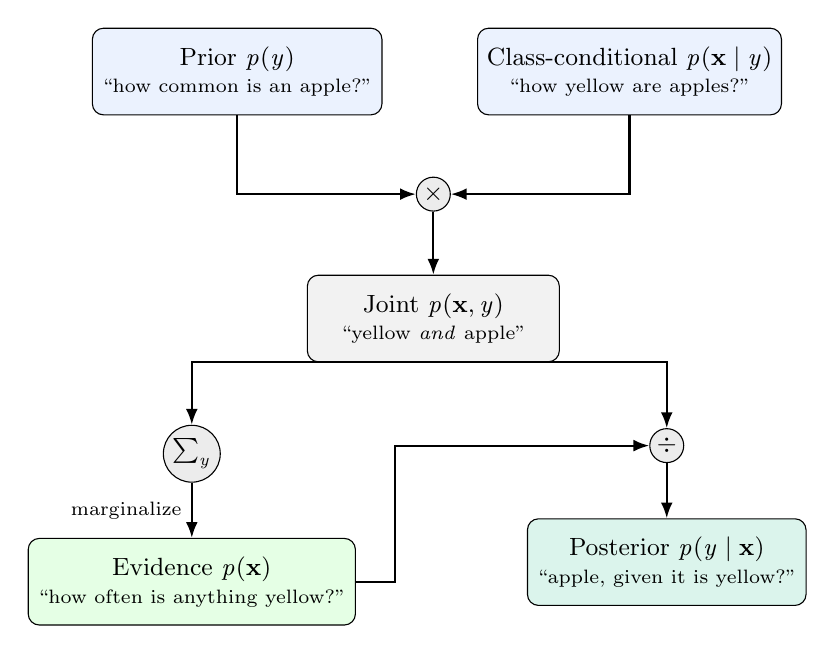
\begin{tikzpicture}[
  box/.style={draw,rounded corners,minimum width=3.2cm,minimum height=1.1cm,align=center,font=\small},
  op/.style={circle,draw,fill=gray!15,inner sep=1pt,font=\small},
  ar/.style={-{Latex[length=2mm]},thick}]
\node[box,fill=cA!10]  (prior) {Prior $p(y)$\\[-1pt]\scriptsize ``how common is an apple?''};
\node[box,fill=cA!10,right=1.2cm of prior] (lik) {Class-conditional $p(\vect x\mid y)$\\[-1pt]\scriptsize ``how yellow are apples?''};
\node[op] (mul) at ($(prior.south)!0.5!(lik.south)+(0,-1)$) {$\times$};
\node[box,fill=gray!10,below=0.8cm of mul] (joint) {Joint $p(\vect x,y)$\\[-1pt]\scriptsize ``yellow \emph{and} apple''};
\node[op,below left=0.9cm and 1.2cm of joint] (sum) {$\sum_{y}$};
\node[box,fill=green!10,below=0.7cm of sum] (evid) {Evidence $p(\vect x)$\\[-1pt]\scriptsize ``how often is anything yellow?''};
\node[op,below right=0.9cm and 1.2cm of joint] (div) {$\div$};
\node[box,fill=cB!15,below=0.7cm of div] (post) {Posterior $p(y\mid\vect x)$\\[-1pt]\scriptsize ``apple, given it is yellow?''};
\draw[ar] (prior.south) |- (mul);
\draw[ar] (lik.south) |- (mul);
\draw[ar] (mul) -- (joint);
\draw[ar] (joint.south) -| (sum);
\draw[ar] (sum) -- node[left,font=\scriptsize]{marginalize} (evid);
\draw[ar] (joint.south) -| (div);
\draw[ar] (evid.east) -- ++(0.5,0) |- (div.west);
\draw[ar] (div) -- (post);
\end{tikzpicture}
\caption{How the probability terms of Sec.~2.1 are connected via Bayes rule.}
\end{figure}
\subsection{Bayes rule:}

	\begin{eqnarray*}
		\underbrace{p(\vect x , y)}_{\text{joint}}
		&=&   \underbrace{p(y)}_{\text{prior}} \cdot \underbrace{p(\vect x \mid y)}_{\text{class-conditional pdf}} \\
		&=& \underbrace{ p(\vect x)}_{\text{evidence}} \cdot \underbrace{ p(y\mid \vect x)}_{\text{posterior}}
	\end{eqnarray*}
	Now we get the posterior as follows:

	\begin{eqnarray*}
		p(y\mid \vect x)
		&=& \frac{p(y) \cdot p(\vect x \mid y)}{p(\vect x)} \\ 
		&=& \frac{p(y) \cdot p(\vect x \mid y)}{\sum\limits_{y'}p(\vect x , y')} \\ 
		&=& \frac{p(y) \cdot p(\vect x \mid y)}{\sum\limits_{y'}p(y') \cdot p(\vect x \mid y')}\\
	\end{eqnarray*}
	\subsubsection{Note:}
	\begin{displaymath}
		p(\vect x) = \sum\limits_{y}p(y) \cdot p(\vect x \mid y)
	\end{displaymath}
	is a \textbf{marginal} of $p(\vect x , y)$.
	\begin{itemize}
		\item We get $p(\vect{x})$ by marginalizing $p(\vect{x}, y)$ over $y$.
		\item Accordingly we get $p(y)$ by marginalizing $p(\vect{x}, y)$ over $\vect{x}$, i.\,e.
		      \begin{eqnarray*}
			      p(y)&=& \int p(\vect{x}, y) \, \mathsf{d}\vect{x}
		      \end{eqnarray*}
	\end{itemize}
	Now let us summarize the Bayesian decision rule: The optimal prediction $\hat y^*$ is the class with the highest posterior,
	\begin{eqnarray*}
		\hat y^* &=&   \argmax\limits_{y} p(y \mid \vect x) \\
		&=& \argmax_y \frac{p(y) \cdot p(\vect x \mid y)}{p(\vect x)} \\
		&=& \argmax_y p(y) \cdot p(\vect x \mid y) \\
		&=& \argmax_y\{\log p(y)\ + \log p(\vect x \mid y)\} 
	\end{eqnarray*}
	\textbf{Notes:} 
	\begin{itemize}
    \item Understand why the denominator was dropped in the above derivation. 
		\item The key aspect in designing a classifier is to find a good model for the posterior $p(y\mid\vect x)$.
		\item Feature vectors $\vect x$ usually have fixed dimension $d$ in simple classification schemes,
		\item but ${\mathcal{X}}$ is not necessarily a subset of $\mathbb{R}^d$: features of varying dimension, sequences and sets of features.
	\end{itemize}

    \begin{figure}[H]\centering
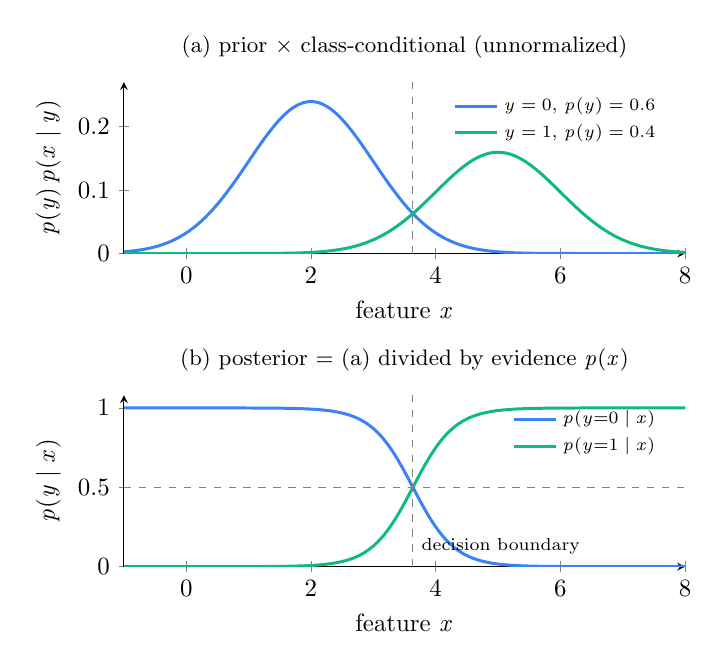
\begin{tikzpicture}[scale=0.9,transform shape]
\begin{groupplot}[group style={group size=1 by 2,vertical sep=2.0cm},
  width=9.5cm,height=4.0cm,domain=-1:8,samples=120,xmin=-1,xmax=8,
  axis lines=left,xlabel={feature $x$},every axis plot/.append style={very thick},
  legend style={draw=none,font=\scriptsize,fill=none},legend pos=north east]
\nextgroupplot[ylabel={$p(y)\,p(x\mid y)$},ymin=0,ymax=0.27,
  title={\small (a) prior $\times$ class-conditional (unnormalized)}]
 \addplot[cA] {0.6*exp(-(x-2)^2/2)/sqrt(2*pi)}; \addlegendentry{$y=0$, $p(y)=0.6$}
 \addplot[cB] {0.4*exp(-(x-5)^2/2)/sqrt(2*pi)}; \addlegendentry{$y=1$, $p(y)=0.4$}
 \draw[dashed,gray] (axis cs:3.635,0)--(axis cs:3.635,0.27);
\nextgroupplot[ylabel={$p(y\mid x)$},ymin=0,ymax=1.08,
  title={\small (b) posterior = (a) divided by evidence $p(x)$}]
 \addplot[cA] {1/(1+ (0.4*exp(-(x-5)^2/2))/(0.6*exp(-(x-2)^2/2)))}; \addlegendentry{$p(y{=}0\mid x)$}
 \addplot[cB] {1/(1+ (0.6*exp(-(x-2)^2/2))/(0.4*exp(-(x-5)^2/2)))}; \addlegendentry{$p(y{=}1\mid x)$}
 \draw[dashed,gray] (axis cs:-1,0.5)--(axis cs:8,0.5);
 \draw[dashed,gray] (axis cs:3.635,0)--(axis cs:3.635,1.08) node[pos=0.12,right,font=\scriptsize,black]{decision boundary};
\end{groupplot}
\end{tikzpicture}
\caption{Bayes rule. The posteriors always sum to one; the class with the larger $p(y)\,p(x\mid y)$ wins.}
\end{figure}

\begin{figure}[H]\centering
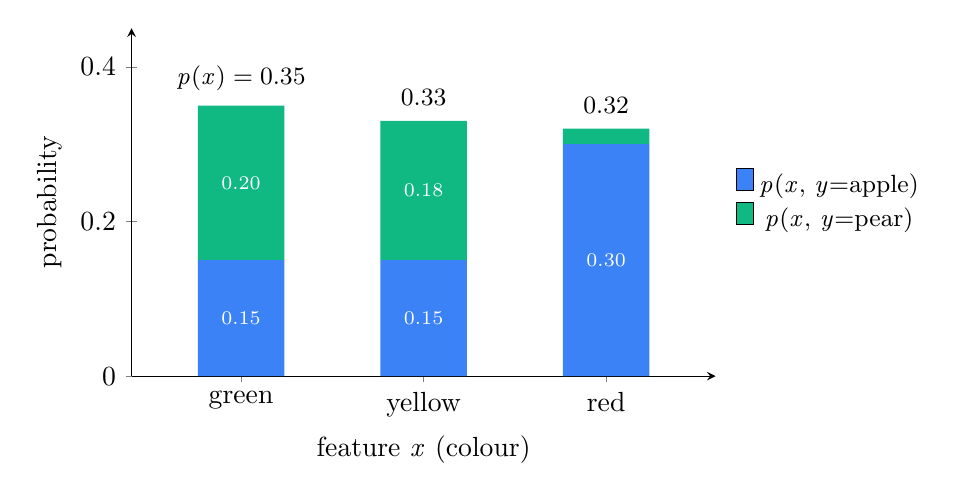
\begin{tikzpicture}
\begin{axis}[ybar stacked,bar width=1.1cm,width=9cm,height=6cm,ymin=0,ymax=0.45,
  xmin=0.4,xmax=3.6,xtick={1,2,3},xticklabels={green,yellow,red},
  xlabel={feature $x$ (colour)},ylabel={probability},axis lines=left,
  legend style={draw=none,font=\small,at={(1.02,0.5)},anchor=west},
  after end axis/.code={% segment labels drawn on top of the bars
   \node[font=\scriptsize,white] at (axis cs:1,0.075) {0.15};
   \node[font=\scriptsize,white] at (axis cs:2,0.075) {0.15};
   \node[font=\scriptsize,white] at (axis cs:3,0.15)  {0.30};
   \node[font=\scriptsize,white] at (axis cs:1,0.25) {0.20};
   \node[font=\scriptsize,white] at (axis cs:2,0.24) {0.18};}]
 \addplot[fill=cA,draw=none] coordinates {(1,0.15) (2,0.15) (3,0.30)};
 \addlegendentry{$p(x,\,y{=}\text{apple})$}
 \addplot[fill=cB,draw=none] coordinates {(1,0.20) (2,0.18) (3,0.02)};
 \addlegendentry{$p(x,\,y{=}\text{pear})$}
 \node[above=2pt,font=\small] at (axis cs:1,0.35) {$p(x)=0.35$};
 \node[above=2pt,font=\small] at (axis cs:2,0.33) {$0.33$};
 \node[above=2pt,font=\small] at (axis cs:3,0.32) {$0.32$};
\end{axis}
\end{tikzpicture}
\caption{Marginalization: the total bar height is $p(x)=\sum_y p(x,y)$. Summing one colour across all bars gives $p(y)$ (apple $0.6$, pear $0.4$). The posterior is a bar's segment over its total, e.g.\ $p(\text{apple}\mid\text{yellow})=0.15/0.33$.}
\end{figure}

	\subsection{Types of models}
	There are two main types of classifiers or models. 
	\begin{itemize}
		\item \textbf{Generative modeling:}  modeling and estimation of $p(y)$ and $p(\vect x | y)$. 
		Where the model tries to estimate the actual sample and hence needs knowledge of the feature space and also how to generate new samples in that feature space.
		\item \textbf{Discriminative modeling:} straight modeling and estimation of $p(y|\vect x)$. Where the model only needs to understand the difference between the two feature spaces, and does not need to know how to generate new samples. It can only discriminate between classes, cannot generate new information. 
	\end{itemize}

\noindent 
\textbf{Notes:} In this chapter, we discuss Bayesian classifiers which are generative models. The explanation of the discriminative models are given to contrast the definition only. 

\begin{figure}[H]\centering
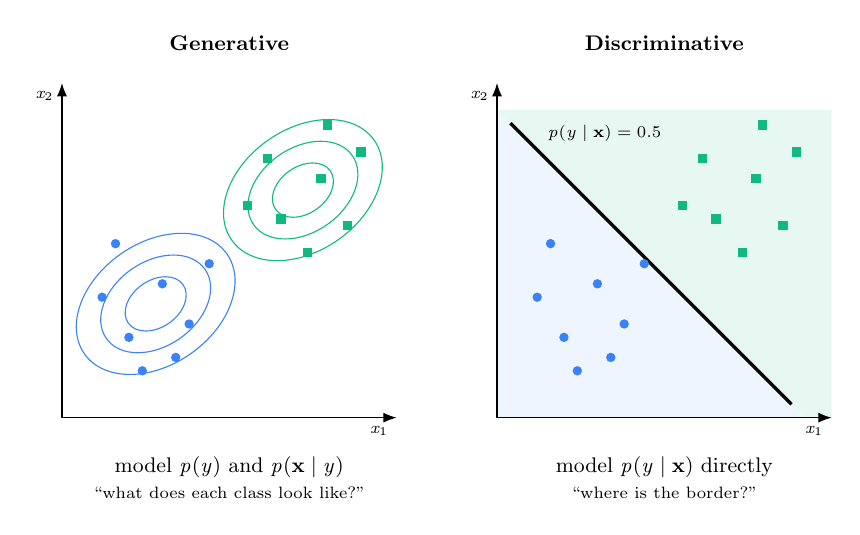
\begin{tikzpicture}[scale=0.85,transform shape]
\def\pts{
 \foreach \x/\y in {1.0/1.2,1.5/2.0,0.6/1.8,1.9/1.4,1.2/0.7,2.2/2.3,0.8/2.6,1.7/0.9}
   {\fill[cA] (\x,\y) circle (2pt);}
 \foreach \x/\y in {3.2/2.9,3.8/3.5,3.0/3.8,4.2/2.8,3.6/2.4,4.4/3.9,2.7/3.1,3.9/4.3}
   {\fill[cB] (\x,\y) rectangle ++(4pt,4pt);}}
\begin{scope}
 \draw[-{Latex}] (0,0)--(5,0) node[below left,font=\scriptsize]{$x_1$};
 \draw[-{Latex}] (0,0)--(0,5) node[below left,font=\scriptsize]{$x_2$};
 \foreach \s in {0.5,0.9,1.3}{
  \draw[cA,rotate around={35:(1.4,1.7)}] (1.4,1.7) ellipse ({\s*1.0} and {\s*0.7});
  \draw[cB,rotate around={35:(3.6,3.4)}] (3.6,3.4) ellipse ({\s*1.0} and {\s*0.7});}
 \pts
 \node[font=\small\bfseries] at (2.5,5.6) {Generative};
 \node[font=\small,align=center] at (2.5,-0.9) {model $p(y)$ and $p(\vect x\mid y)$\\ \scriptsize ``what does each class look like?''};
\end{scope}
\begin{scope}[xshift=6.5cm]
 \fill[cA!8] (0,0)--(0,4.6)--(4.6,0)--cycle;
 \fill[cB!10] (0,4.6)--(5,4.6)--(5,0)--(4.6,0)--cycle;
 \draw[-{Latex}] (0,0)--(5,0) node[below left,font=\scriptsize]{$x_1$};
 \draw[-{Latex}] (0,0)--(0,5) node[below left,font=\scriptsize]{$x_2$};
 \draw[very thick] (0.2,4.4)--(4.4,0.2) node[pos=0.1,above right,font=\scriptsize]{$p(y\mid\vect x)=0.5$};
 \pts
 \node[font=\small\bfseries] at (2.5,5.6) {Discriminative};
 \node[font=\small,align=center] at (2.5,-0.9) {model $p(y\mid\vect x)$ directly\\ \scriptsize ``where is the border?''};
\end{scope}
\end{tikzpicture}
\caption{Same data, two strategies. Generative models describe each class (and can sample new data); discriminative models only learn the boundary.}
\end{figure}

\subsection{Optimality of the Bayesian Classifier}

A loss function quantifies the cost associated with making a decision, particularly when the decision is incorrect. Different types of classification errors may have different consequences, and the loss function allows us to express these consequences numerically. For a given decision rule, we can compute the expected loss over many samples. The best classifier is then the one that minimizes this expected loss. When all classification errors are assigned the same cost, minimizing the expected loss reduces to minimizing the classification error rate.

\begin{figure}[H]\centering
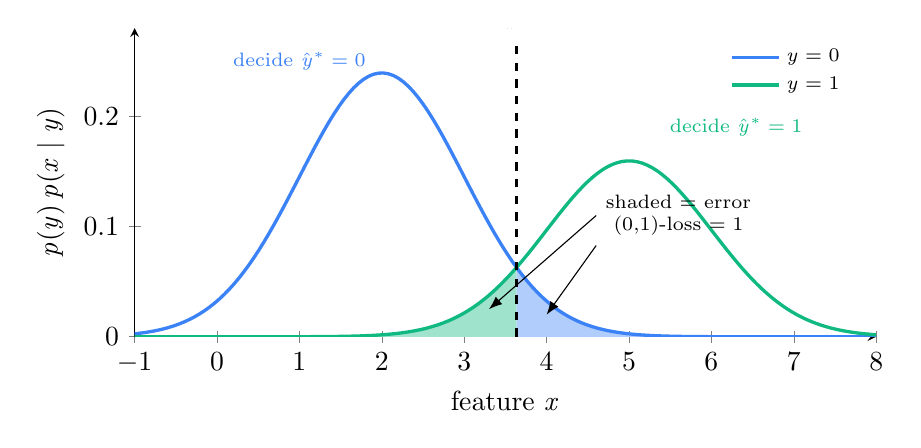
\begin{tikzpicture}
\begin{axis}[width=11cm,height=5.5cm,domain=-1:8,samples=150,xmin=-1,xmax=8,ymin=0,ymax=0.28,
  axis lines=left,xlabel={feature $x$},ylabel={$p(y)\,p(x\mid y)$},
  legend style={draw=none,font=\scriptsize,fill=none},legend pos=north east]
 \addplot[cA,very thick,name path=A] {0.6*exp(-(x-2)^2/2)/sqrt(2*pi)}; \addlegendentry{$y=0$}
 \addplot[cB,very thick,name path=B] {0.4*exp(-(x-5)^2/2)/sqrt(2*pi)}; \addlegendentry{$y=1$}
 \path[name path=ax] (axis cs:-1,0)--(axis cs:8,0);
 \addplot[cB!40] fill between[of=B and ax,soft clip={domain=-1:3.635}];
 \addplot[cA!40] fill between[of=A and ax,soft clip={domain=3.635:8}];
 \draw[thick,dashed] (axis cs:3.635,0)--(axis cs:3.635,0.27) node[above,font=\scriptsize]{$x^*$};
 \node[font=\scriptsize,cA] at (axis cs:1,0.25) {decide $\hat y^*=0$};
 \node[font=\scriptsize,cB] at (axis cs:6.3,0.19) {decide $\hat y^*=1$};
 \node[font=\scriptsize,align=center] (e) at (axis cs:5.6,0.11) {shaded = error\\(0,1)-loss $=1$};
 \draw[-{Latex},thin] (e.south west)--(axis cs:4.0,0.02);
 \draw[-{Latex},thin] (e.west)--(axis cs:3.3,0.025);
\end{axis}
\end{tikzpicture}
\caption{The Bayes classifier $\hat y^*=\arg\max_y p(y\mid\vect x)$ places the boundary where the curves cross. $x^*$ is the crossing point, i.\,e.\ the decision boundary. Moving it in either direction only adds shaded area, so no other rule has a lower expected (0,1)-loss.}
\end{figure}
	
$l(y',y)$ is the \textbf{loss} of assigning true class $y$ to class $y'$. The $(0,1)$-loss function is defined by
		\begin{eqnarray*}
			l(y',y) &= &\left\{ \begin{array}{ll}
				0 & \text{if } y'=y \\
				1 & \text{otherwise}
			\end{array} \right.
		\end{eqnarray*}

\noindent
The \textbf{best (optimal) decision rule} minimizes the expected loss
\begin{eqnarray*}
	\mathsf{AL}(\vect x , y') &=& \sum\limits_{y} l(y',y)\,p(y\mid\vect x),
\end{eqnarray*}
where the true class is unknown, so we average over its posterior.

Using the $(0,1)$-loss, the optimal prediction is
	\begin{eqnarray*}
		\hat y^* &=& \argmin\limits_{y'} \mathsf{AL}(\vect x, y')\\
		        &=& \argmin\limits_{y'} \left(1-p(y'\mid\vect x)\right)\\ 
		        &=& \argmax\limits_{y'} p(y'\mid\vect x).\\
	\end{eqnarray*}
	
	\subsection{Conclusion}

	\begin{itemize}
		\item The optimal classifier w.\,r.\,t.\ the (0,1)-loss function applies the Bayesian decision rule.
		\item This classifier is called \textbf{Bayesian classifier}. The Bayesian classifier is an ideal classifier that is mostly impossible to achieve in reality.  
	\end{itemize}
	

    \noindent
    \vorsicht The $(0,1)$-loss function is {\bf NOT} convex. Hence optimizing this loss function in practical scenario is very difficult 

\begin{figure}[H]\centering
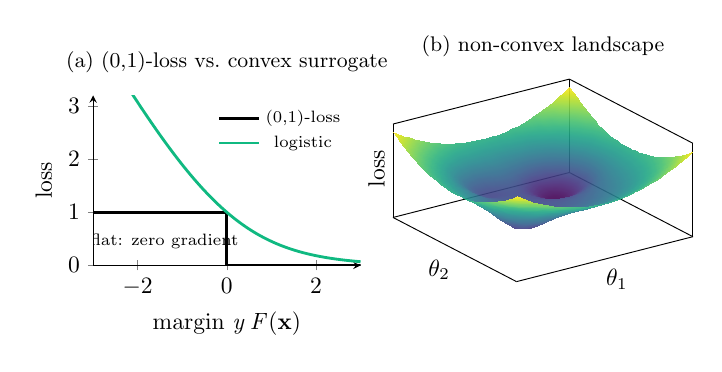
\begin{tikzpicture}[scale=0.85,transform shape]
\begin{axis}[name=l,width=0.46\linewidth,height=0.34\linewidth,xmin=-3,xmax=3,ymin=0,ymax=3.2,axis lines=left,
  xlabel={margin $y\,F(\vect x)$},ylabel={loss},title={\small (a) (0,1)-loss vs.\ convex surrogate},
  legend style={draw=none,font=\scriptsize,fill=none},legend pos=north east]
 \addplot[black,very thick,const plot] coordinates {(-3,1) (0,1) (0,0) (3,0)}; \addlegendentry{(0,1)-loss}
 \addplot[cB,very thick,domain=-3:3,samples=80] {ln(1+exp(-x))/ln(2)}; \addlegendentry{logistic}
 \node[font=\scriptsize,align=center] at (axis cs:-1.4,0.45) {flat: zero gradient};
\end{axis}
\begin{axis}[at={(l.east)},anchor=west,xshift=0.04\linewidth,width=0.50\linewidth,height=0.38\linewidth,view={-35}{40},
  domain=-3:3,y domain=-3:3,samples=35,colormap/viridis,
  xlabel={$\theta_1$},ylabel={$\theta_2$},zlabel={loss},ticks=none,
  title={\small (b) non-convex landscape}]
 \addplot3[surf,shader=interp,opacity=0.9]
   {0.15*(x^2+y^2) - 1.3*exp(-((x-1.3)^2+(y-1.2)^2)) - 0.8*exp(-((x+1.4)^2+(y+0.9)^2)/0.8) - 0.6*exp(-((x+1)^2+(y-1.6)^2)/0.6)};
\end{axis}
\end{tikzpicture}
\caption{(a) The (0,1)-loss is a step: non-convex with zero gradient almost everywhere, so it cannot be minimized by gradient methods. (b) A non-convex landscape has several local minima; the result depends on initialization.}
\end{figure}

	\subsection{Lessons Learned}
\begin{itemize}
		\item General structure of a classification system 
		\item Supervised and unsupervised learning  
		\item Basics on probabilities (probability, pdf, Bayes rule, etc.)  
		\item Optimality of Bayes classifier and the role of the loss function   
		\item Discriminative and generative approach to model a posteriori probability
	\end{itemize}

\clearpage

\newpage

\section{Logistic regression}

Despite its name, logistic regression is a \textbf{classification} method: it models the posterior $p(y\mid\vect x)$ directly by a logistic (sigmoid) function, and its parameters are estimated by maximizing the log-likelihood (Sec.~\ref{sec:lr_learning}). The name comes from regressing the log-odds on the features. Compare: in \emph{regression} a continuous value is predicted (e.g.\ the exact size of a flower), in \emph{classification} only the class (flower A or B).\autocite{hastie2009,bishop2006}

\subsection{Posteriors and the Logistic Function}

\begin{figure}
    \centering
    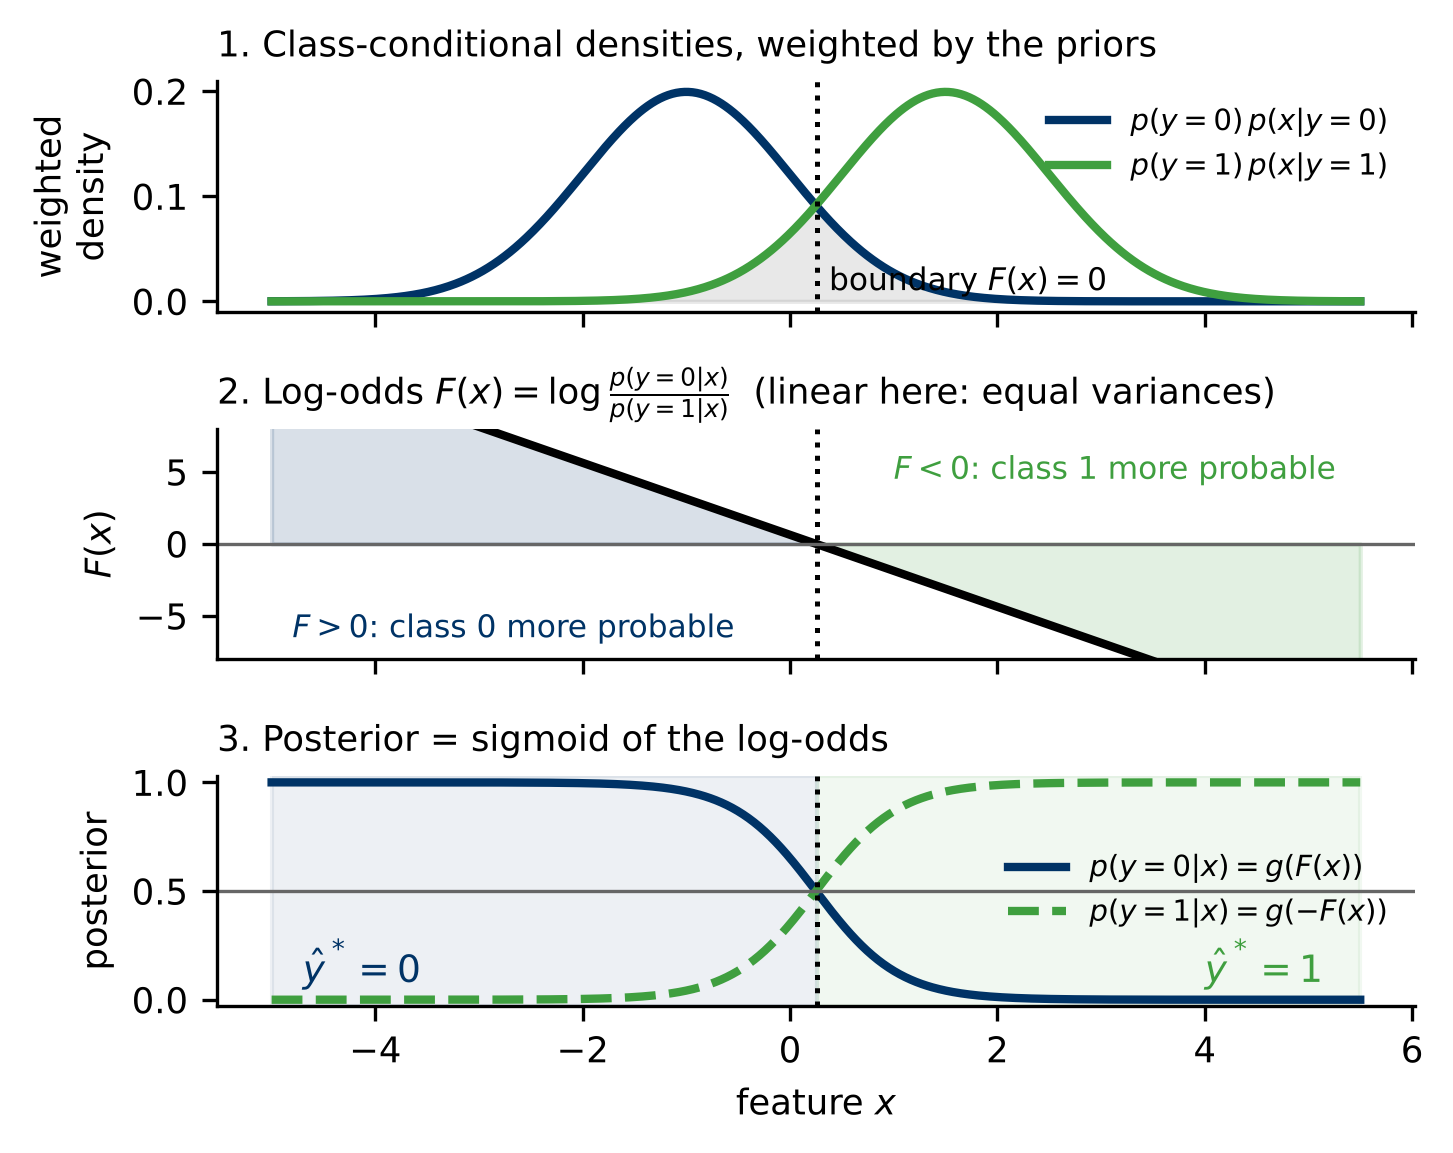
\includegraphics[width=0.75\linewidth]{ch03_densities_logodds_posterior.png}
    \caption{From class-conditional densities to the posterior for 1-D Gaussians with $\mu_0=-1$, $\mu_1=1.5$, $\sigma=1$, equal priors.}
    \label{fig:logodds_posterior}
\end{figure}

For two classes $y\in\{0, 1\}$ we get:
  
  \begin{eqnarray*}
    p(y=0\mid \vect x)
      &=&  \frac{p(y=0)\, p(\vect x \mid y=0)}{p(\vect x)} \\ 
      &=& \frac{p(y=0)\, p(\vect x \mid y=0)}{p(y=0)p(\vect x \mid y=0)+p(y=1)p(\vect x \mid y=1)} \\
      &=& \frac{1}{1+\frac{p(y=1)p(\vect x\mid y=1)}{p(y=0)p(\vect x\mid y=0)}} \\
      &\phantom{=}& \mbox{\small (\textbf{Trick:} extend with exponential and logarithm)} \\ 
      &=& \frac{1}{1+e^{\log \frac{p(y=1)p(\vect x\mid y=1)}{p(y=0)p(\vect x\mid y=0)}}} \\
      &=& \frac{1}{1+e^{-\log\frac{p(y=0)}{p(y=1)} - \log\frac{p(\vect x\mid y=0)}{p(\vect x\mid y=1)}}}\\
      &=& \frac{1}{1+e^{-\log\frac{p(y=0\mid\vect x)}{p(y=1\mid\vect x)}}}.
  \end{eqnarray*}
 We see that the posterior for class $y = 0$ can be written in terms of a \textbf{logistic function}. Define
\begin{eqnarray*}
  F(\vect x) := \log\frac{p(y=0\mid\vect x)}{p(y=1\mid\vect x)}
\end{eqnarray*}
(i.e.\ $F$ is the log-odds of class $0$ vs.\ class $1$). Then
 \begin{eqnarray*}
    p(y=0\mid \vect x) &=& \frac{1}{1+e^{-F(\vect{x})}}.
  \end{eqnarray*}
  And thus the posterior for the other class $y = 1$:
  \begin{eqnarray*}
    p(y=1\mid \vect x) &=& 1- p(y=0\mid \vect x) \\
                   &=& \frac{e^{-F(\vect x)}}{1+e^{-F(\vect{x})}} \\
                   &=&  \frac{1}{1+e^{F(\vect{x})}}.
  \end{eqnarray*}
The {\em logistic function} (also called {\em sigmoid function}) is defined by
    \begin{eqnarray*}
      g(z) &=& \frac{1}{1+e^{-z}},
    \end{eqnarray*}
    where $z\in \mathbb{R}$ (a scalar, not a feature vector).
    
The reason we have transformed into this kind of logistic or sigmoid function, is because it fulfills this nice derivative property which will help us in the following chapters. The derivative is given by:
  \begin{eqnarray*}
    g'(z) &=& \left( \frac{1}{1+e^{-z}} \right)' = \left( (1+e^{-z})^{-1}\right)'=  \frac{1}{(1+e^{-z})^2}\cdot e^{-z} \\ 
          &=& \frac{1}{(1+e^{-z})} \cdot \frac{e^{-z}}{(1+e^{-z})} \\
          &=& \frac{1}{(1+e^{-z})} \cdot \frac{1}{(1+e^{z})} \\
          &=& g(z)g(-z) \\
          &=& g(z)(1-g(z)) \quad.
  \end{eqnarray*}

  \begin{figure}
      \centering
      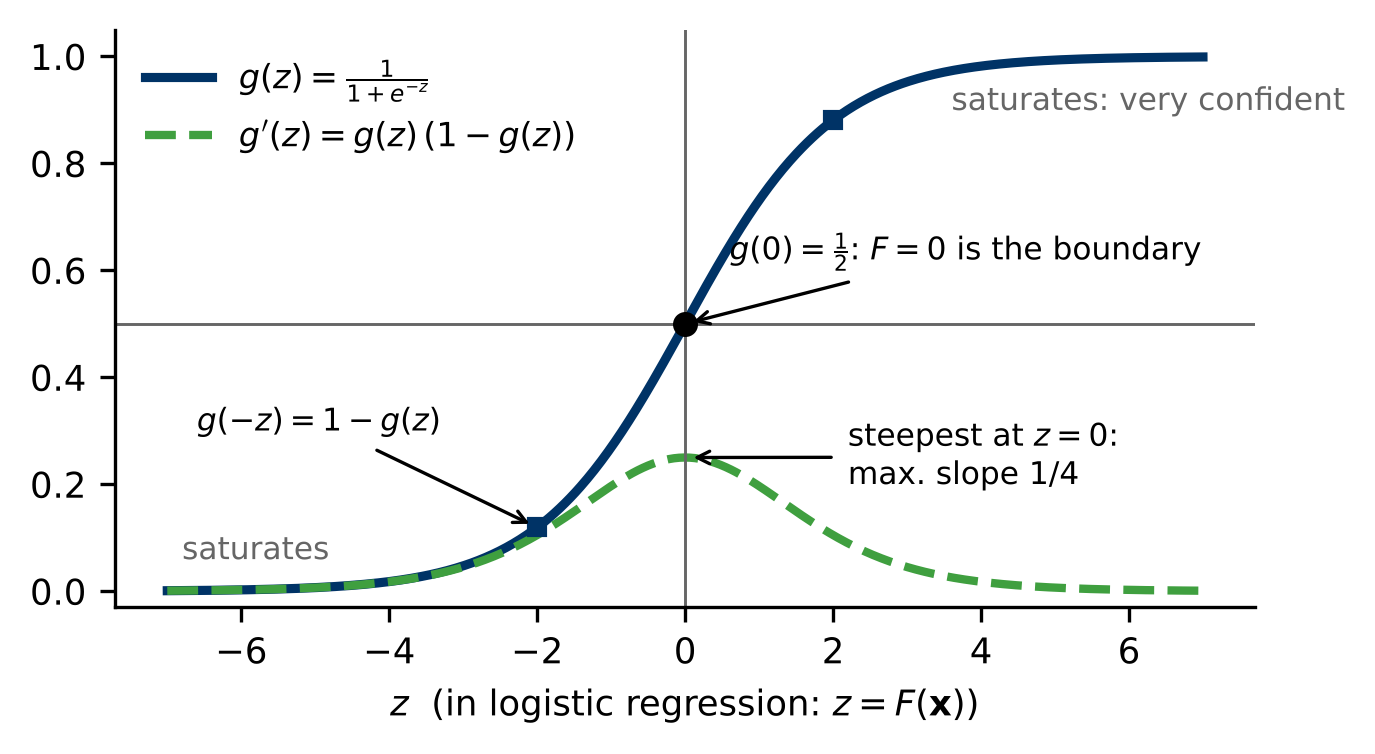
\includegraphics[width=0.75\linewidth]{ch03_sigmoid_properties.png}
      \caption{Logistic (sigmoid) function $g(z)=\frac{1}{1+e^{-z}}$ and its derivative $g'(z)=g(z)(1-g(z))$.}
      \label{fig:sigmoid_properties}
  \end{figure}
  \subsection{Decision Boundary}
    The \textbf{decision boundary} in feature space separates the regions where the classifier decides for class $0$ and class $1$. On the boundary, the posterior probabilities are equal; for the two-class case this means $p(y=0\mid\vect x)=p(y=1\mid\vect x)=0.5$.
  Points $\vect x$ on the decision boundary satisfy:
 
  \begin{eqnarray*}
    {p(y=0|\vect{x})}&=& {p(y=1|\vect x)}
  \end{eqnarray*}
  and thus
  \begin{eqnarray*}
    \log \frac{p(y=0|\vect{x})}{p(y=1|\vect x)} &=& \log 1 = 0 \quad.
  \end{eqnarray*}
  The lemma below makes the decision-boundary condition explicit.
  \begin{lemma}
    The decision boundary is given by $F(\vect x)=0$.
  \end{lemma}
  \textbf{Proof:} By definition, $F(\vect x)=\log\frac{p(y=0\mid\vect x)}{p(y=1\mid\vect x)}$. Hence
  \begin{eqnarray*}
    F(\vect x)=0
    &\Leftrightarrow& \log\frac{p(y=0\mid\vect x)}{p(y=1\mid\vect x)}=0 \\
    &\Leftrightarrow& \frac{p(y=0\mid\vect x)}{p(y=1\mid\vect x)}=1 \\
    &\Leftrightarrow& p(y=0\mid\vect x)=p(y=1\mid\vect x).
  \end{eqnarray*}

  Since $p(y=0\mid\vect x)+p(y=1\mid\vect x)=1$, we get $p(y=0\mid\vect x)=p(y=1\mid\vect x)=\tfrac{1}{2}$ if and only if $F(\vect x)=0$.


  \subsection{Decision Rule}
  The classifier predicts class $0$ if the posterior of class $0$ is larger than $\tfrac{1}{2}$, i.\,e. if $F(\vect x)>0$:
  \begin{eqnarray*}
    \hat y^* &=& \left\{\begin{array}{ll}
      0 & \text{if } F(\vect x) > 0 \\
      1 & \text{if } F(\vect x) < 0
    \end{array}\right.
  \end{eqnarray*}
  The boundary is given by $F(\vect x)=0$. Note that $\hat y^*$ is the predicted class; the true class $y$ (or labels $y_i$ in the training set) can differ.

\begin{figure}
    \centering
    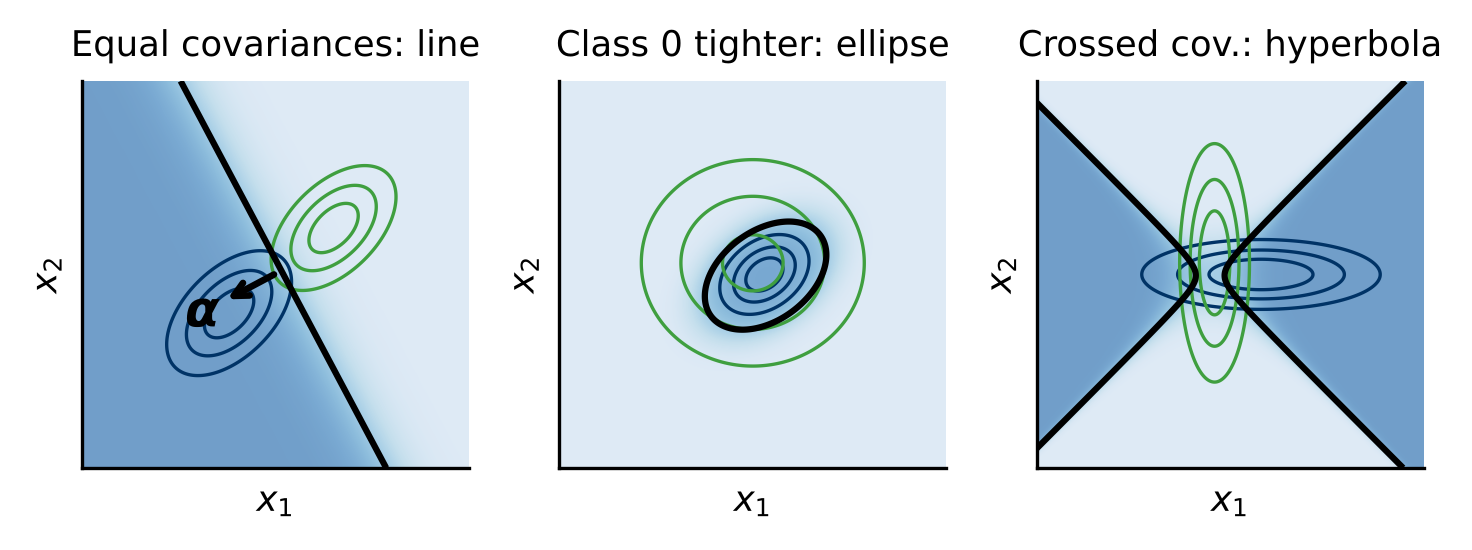
\includegraphics[width=0.8\linewidth]{ch03_2d_boundaries.png}
    \caption{Decision boundaries $F(\vect x)=0$ for two 2-D Gaussian classes: equal covariances give a line; unequal covariances give conic sections.}
    \label{fig:boundaries}
\end{figure}
 \subsubsection{Example}
    \textbf{Note:} Important to understand this example and derivation. Forms the foundation of future chapters. Let us assume both classes have normally distributed $d$-dimensional feature vectors:
    \begin{eqnarray*}
      p(\vect x \mid y) &=& \mathcal N(\vect x;\vect\mu_y,\mat\Sigma_y)
      = \frac{1}{\sqrt{\det(2\pi \mat\Sigma_y)}}
        e^{-\frac{1}{2} (\vect{x} - \vect{\mu}_y)^T \mat\Sigma_y^{-1} (\vect{x} - \vect{\mu}_y)}
    \end{eqnarray*}
    where $\mat\Sigma_y$ is the covariance matrix and $\vect\mu_y$ the mean of class $y$. This convention is followed throughout the document. 
 
    Then we can write the posterior of $y=0$ in terms of a logistic function:
 
    \begin{eqnarray*}
      p(y=0|\vect x) &=& \frac{1}{1+e^{-F(\vect x)}} = \frac{1}{1+e^{ - \left( \vect x^T \mat A \vect x + \vect \alpha^T\vect x + \alpha_0 \right) } } \\ \\
      F(\vect x) &=& \log \frac{p(y=0|\vect x)}{p(y=1|\vect x)} = \log \frac{p(y=0)p(\vect x | y=0) }{p(y=1)p(\vect x|y =1)}\\
      F(\vect x) &=&
        \log\frac{p(y=0)}{p(y=1)} +
        \log
        \frac{
          \frac{1}{ \sqrt{ \det{( 2 \pi \mat{\Sigma}_0)}} }
          e^{ -\frac{1}{2} (\vect{x} - \vect{\mu}_0)^T \mat{\Sigma}_0^{-1} (\vect{x} - \vect{\mu}_0) }         
        }{
          \frac{1}{ \sqrt{ \det{(2 \pi \mat{\Sigma}_1)}} }
          e^{ -\frac{1}{2} (\vect{x} - \vect{\mu}_1)^T \mat{\Sigma}_1^{-1} (\vect{x} - \vect{\mu}_1)}
        }
    \end{eqnarray*}
  This function has the constant component (it becomes part of $\alpha_0$ below):
% 
    \begin{eqnarray*}
      \log \frac{p(y=0)}{p(y=1)}+\frac{1}{2}
            \log \frac{ { \det{(2\pi\mat{\Sigma}_1)}}}
                      { { \det{(2\pi\mat{\Sigma}_0)}}}
    \end{eqnarray*}
     We observe:
    \begin{itemize}
      \small
      \item Priors imply a constant offset of the decision boundary. 
      \item If priors and covariance matrices of both classes are identical, this offset is $0$.
    \end{itemize}

   \begin{figure}
       \centering
       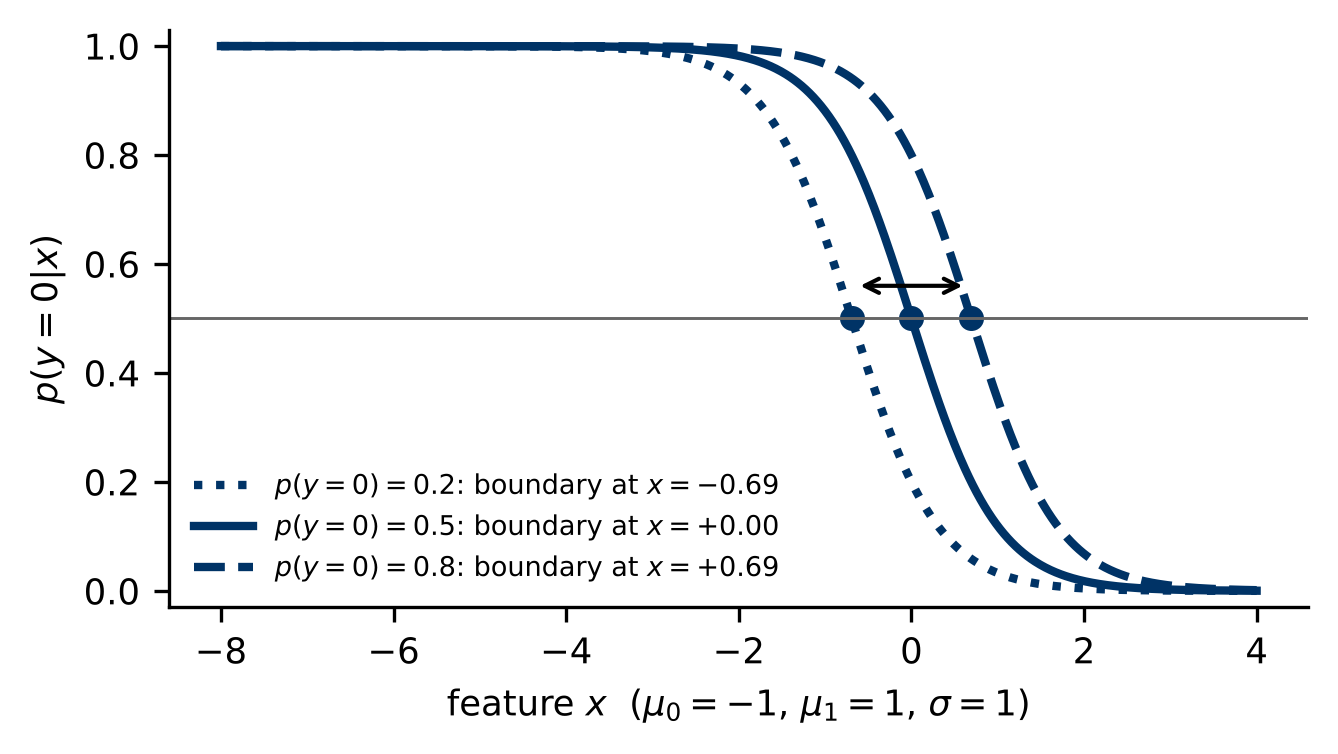
\includegraphics[width=0.75\linewidth]{ch03_prior_shift.png}
       \caption{Effect of the prior on the decision boundary for 1-D Gaussians with $\mu_0=-1$, $\mu_1=1$, $\sigma=1$. Changing $p(y=0)$ shifts the posterior and moves the decision boundary.}
       \label{fig:prior_shift}
   \end{figure}
   Furthermore we have:
    {\small
    \begin{eqnarray*}
      \log{ 
        \frac{e^{ - \frac{1}{2} (\vect{x} - \vect{\mu}_0)^T \mat{\Sigma}_0^{-1} (\vect{x} - \vect{\mu}_0)} }
             {e^{ - \frac{1}{2} (\vect{x} - \vect{\mu}_1)^T \mat{\Sigma}_1^{-1} (\vect{x} - \vect{\mu}_1)} }
      } & = & 
      \frac{1}{2} 
      \left(
        (\vect{x} - \vect{\mu}_1)^T \mat{\Sigma}_1^{-1} (\vect{x} - \vect{\mu}_1) - (\vect{x} - \vect{\mu}_0)^T \mat{\Sigma}_0^{-1} (\vect{x} - \vect{\mu}_0)
      \right) \\
      & &  =
      \frac{1}{2} 
      \left(
        \vect{x}^T (\mat{\Sigma}_1^{-1} - \mat{\Sigma}_0^{-1}) \vect{x} 
        -2 (\vect{\mu}_1^T \mat{\Sigma}_1^{-1} - \vect{\mu}_0^T \mat{\Sigma}_0^{-1} ) \vect{x} + \right.\\
        & & \left.  
        + \vect{\mu}_1^T \mat{\Sigma}_1^{-1} \vect{\mu}_1 - \vect{\mu}_0^T \mat{\Sigma}_0^{-1} \vect{\mu}_0
      \right)
    \end{eqnarray*}
    }
     Now we have:
    \begin{eqnarray*}
      \mat{A}        &=& \frac{1}{2} (\mat{\Sigma}_1^{-1} - \mat{\Sigma}_0^{-1}) \\[.5cm]
      \vect{\alpha}^T &=& \vect{\mu}_0^T \mat{\Sigma}_0^{-1} - \vect{\mu}_1^T \mat{\Sigma}_1^{-1} \\
      \alpha_0       &=& \log \frac{p(y=0)}{p(y=1)} + \frac{1}{2}
                         \left(
                           \log
                             \frac{ \det{( 2 \pi \mat{\Sigma}_1)}}
                                  { \det{( 2 \pi \mat{\Sigma}_0)}} + 
                             \vect{\mu}_1^T \mat{\Sigma}_1^{-1} \vect{\mu}_1 -
                             \vect{\mu}_0^T \mat{\Sigma}_0^{-1} \vect{\mu}_0
                         \right)
    \end{eqnarray*}
    \subsubsection{Properties}
    Quadratic polynomials in the 2 variables $x_1$ and $x_2$\\
    This means if the two variables have a quadratic polynomial relationship with each other. This section is important to understand. 
    
   \begin{eqnarray*}
    F(\vect{x}) 
      &=& \vect x^T \mat A \vect x + \vect \alpha^T\vect x + \alpha_0 \\
      &=& a_{11}x_1^2 + (a_{12}+a_{21})x_1x_2 + a_{22}x_2^2 + \alpha_1 x_1 + \alpha_2 x_2 + \alpha_0 \stackrel{!}{=} 0
  \end{eqnarray*}\\
  \textbf{Posterior probability: } 
  The posterior probability impacts the decision boundary. Below is some of the impacts explained. \\
  
  \subsubsection{Distributions with Equal Dispersion}
    If both classes share the same covariance, i.\,e.\ $\mat\Sigma= \mat\Sigma_0=\mat\Sigma_1$, then the argument $F(\vect x)$ of the sigmoid function is \textbf{affine} in $\vect{x}$.
    \begin{eqnarray*}
      \mat{A}        &=& \mat{0} \\
      \vect{\alpha}^T &=& (\vect{\mu}_0 - \vect{\mu}_1)^T \mat{\Sigma}^{-1} \\
      \alpha_0       &=& \log \frac{p(y=0)}{p(y=1)} +
                         \frac{1}{2}(\vect{\mu}_1 + \vect{\mu}_0)^T \mat{\Sigma}^{-1} (\vect{\mu}_1 - \vect{\mu}_0)
     \end{eqnarray*}
\textbf{Note:}
  \begin{itemize}
    \item If the class conditionals are Gaussians and share the same covariance, the argument of the exponential function is affine in $\vect x$.
    \item This result is even true for a more general family of pdfs and not limited to Gaussians.
  \end{itemize}
 \textbf{Definition}
The {\em exponential family} is a class of pdfs that can be written in the following canonical form
    \begin{eqnarray*}
      p(\vect x;\vect \eta, \phi) &=& e^{\frac{\vect\eta^T \cdot \vect  x -b(\vect \eta)}{a(\phi)}+c(\vect x,\phi)}
    \end{eqnarray*}
    where $\vect \eta\in \mathbb{R}^d$ is the \emph{natural (canonical) parameter vector}, and $\phi$ is the {\em dispersion parameter}. \\
    \textbf{Notation:} parameters are written after \texttt{;} (e.g.\ $p(\vect x;\vect\eta)$), while conditioning uses $\mid$ (e.g.\ $p(\vect x\mid y)$).
  
  \subsubsection{Exponential family of density functions}
  
  When the class-conditional densities $p(\vect x\mid y=0)$ and $p(\vect x\mid y=1)$ belong to the \emph{same} exponential family and share the same dispersion parameter $\phi$, then the log-odds (and hence the decision boundary) is linear in $\vect x$ (see Lemma~2).
  
  \begin{itemize}
      \item {Gaussian probability density function:}
      The class-conditional density for a Gaussian is:
      
     \begin{displaymath}
    \mathcal{N}(\vect{x}; \vect{\mu},\mat{\Sigma}) = \frac{1}{ \sqrt{ \det{(2 \pi \mat{\Sigma})} } }
                    e^{-\frac{1}{2} (\vect{x} - \vect{\mu})^T \mat{\Sigma}^{-1} (\vect{x} - \vect{\mu})  } 
  \end{displaymath}
  \item {Exponential density:}
   \begin{displaymath}
    p(x;\lambda) = \left\{ 
                 \begin{array}{ll}
                   \lambda e^{-\lambda x} & x \ge 0 \\
                   0                      & x < 0 \\
                 \end{array}
               \right.
  \end{displaymath}
  \item {Binomial pmf (success probability $\pi$):}
  \begin{displaymath}
    p(k;n,\pi) = \binom{n}{k} \pi^k (1-\pi)^{n-k}
  \end{displaymath}
  \item {Poisson pmf:}
  \begin{displaymath}
    p(k;\lambda) = \frac{\lambda^k}{k!} e^{-\lambda}
  \end{displaymath}
  \item {Hypergeometric pmf:}
  \begin{displaymath}
    p(k;N,M,n) = \frac{\binom{M}{k}\binom{N-M}{n-k}}{\binom{N}{n}}
  \end{displaymath}
  \end{itemize}

   \begin{lemma}
     If all class-conditional densities are members of the same exponential family of probability density functions with equal dispersion $\phi$, the decision boundary $F(\vect{x})=0$ is linear in the components of $\vect{x}$.
   \end{lemma}
   
   \subsection{Lessons Learned}

  \begin{itemize}
    \item Posteriors can be rewritten in terms of a logistic function. 
    \item Given the decision boundary $F(\vect x)=0$, we can write down the posterior $p(y|\vect x)$ right away.
    \item With class-specific Gaussian covariances, the decision boundary $F(\vect x)=0$ is quadratic in $\vect x$ (a conic section in $d=2$, and a quadric surface in higher dimensions).
    \item If the Gaussian classes share the same covariance matrix, then $F(\vect x)=0$ is linear in $\vect x$, i.e.\ a hyperplane (a straight line only for $d=2$).

\begin{figure}
    \centering
    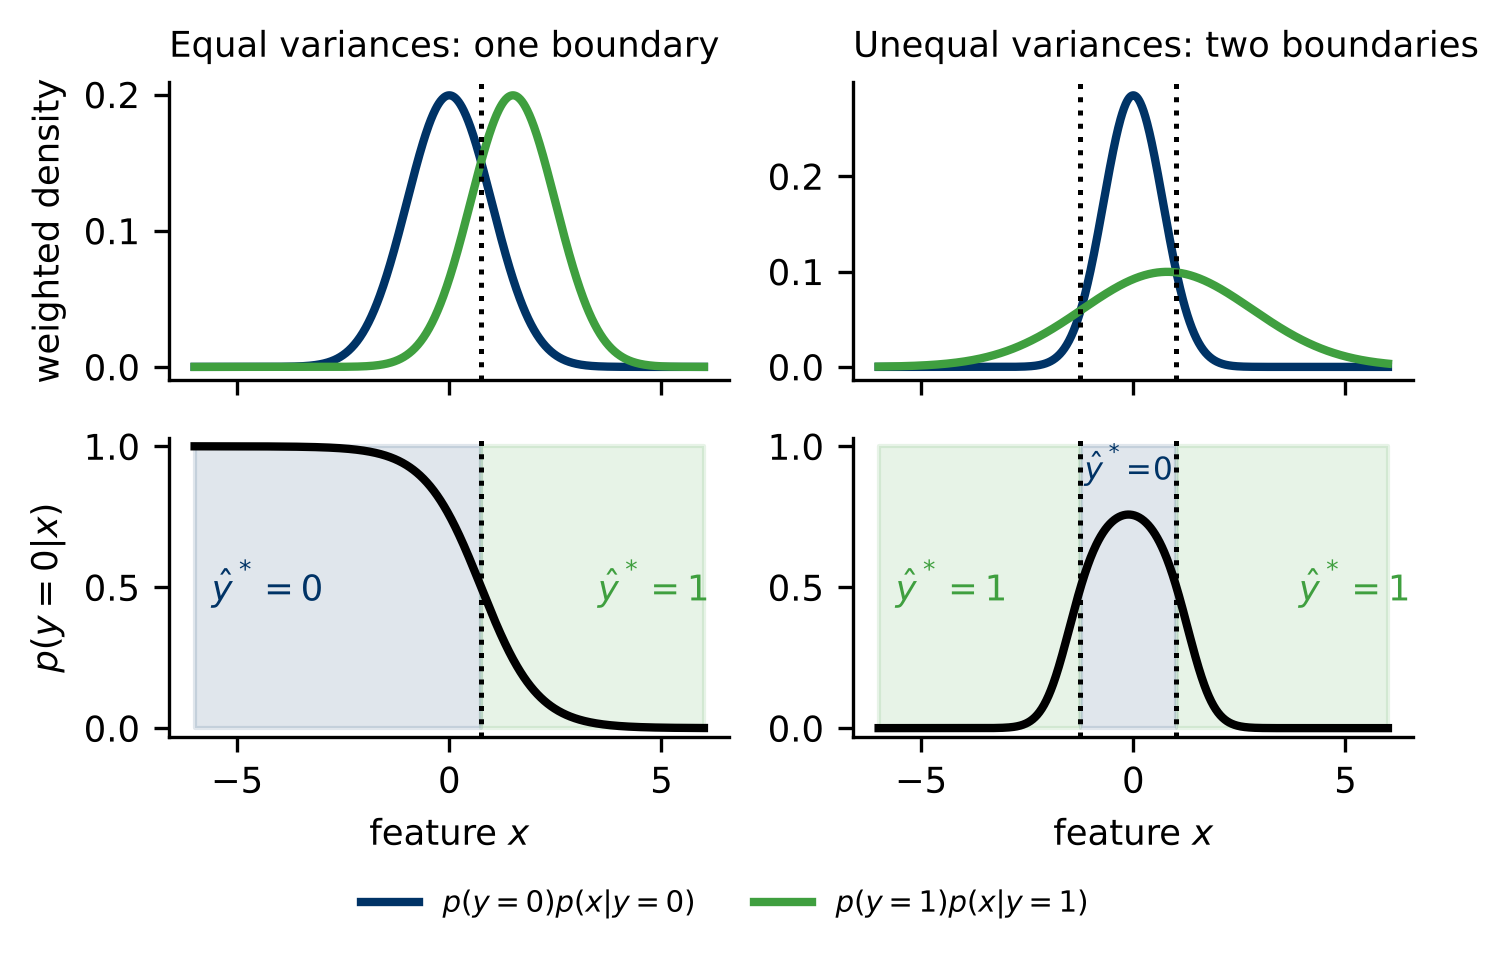
\includegraphics[width=0.75\linewidth]{ch03_equal_vs_unequal_variance.png}
    \caption{Equal vs. unequal variances in 1-D (equal priors): with equal variances $F(x)$ is linear; with unequal variances $F(x)$ is quadratic (and can yield two decision boundaries).}
    \label{fig:unequal_covariances}
\end{figure}
  \end{itemize}
  
\subsection{Parameterization}

Need understanding of linear algebra for this section. 

 \begin{itemize}
    \item Until now, $F(\vect x)$ was some arbitrary function in $\vect x$ \\[.1cm]
      \textbf{Example:} $ F(\vect x) = \vect x^T \mat A \vect x + \vect \alpha^T\vect x + \alpha_0 $ \\[.25cm]
    \item We can express a nonlinear $F(\vect x)$ as a scalar product by lifting $\vect x$ into a higher dimensional space. \\
      Given \\
     $\vect x = \left(x_1, x_2\right)^T \in \real^2,~ \mat A = \left( \begin{array}{cc} a_{11} & a_{12} \\ a_{21} & a_{22} \end{array} \right), ~ \vect \alpha = \left(\alpha_1, \alpha_2 \right)^T, ~\alpha_0 $\,, \\
      then \\
      $F(\vect x) = a_{11} x_1^2 + (a_{12} + a_{21}) x_1 x_2 + a_{22} x_2^2 + \alpha_1 x_1 + \alpha_2 x_2 + \alpha_0$\,.\\[.25cm]
    \item Rewrite $F(\vect x)=\vect a^T\vect x'$ with $\vect a,\vect x' \in \real^6$:
      \\
       $\vect a = (a_{11}, a_{12} + a_{21}, a_{22}, \alpha_1, \alpha_2, \alpha_0)^T$ \\
      $\vect x' = ( x_1^2, x_1 x_2, x_2^2, x_1, x_2, 1)^T$
  \end{itemize}

\begin{figure}[htbp]
  \centering
  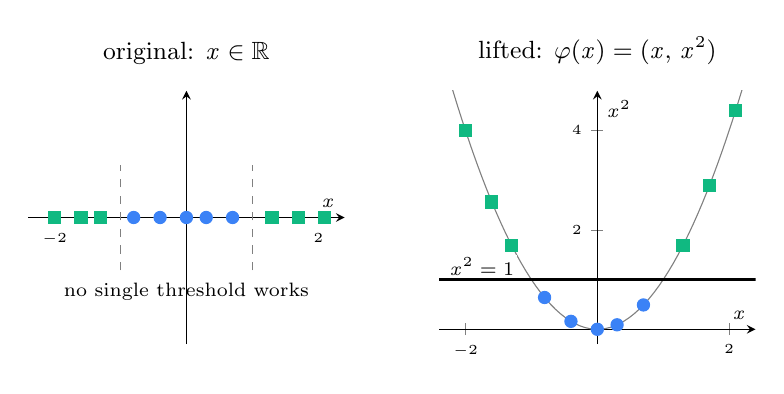
\begin{tikzpicture}
  \begin{groupplot}[group style={group size=2 by 1,horizontal sep=1.2cm},
    width=5.6cm,height=4.8cm,xmin=-2.4,xmax=2.4,axis lines=middle,
    every axis plot/.append style={mark size=2.2pt},
    tick label style={font=\tiny},label style={font=\scriptsize},title style={font=\small}]
  \nextgroupplot[ymin=-0.6,ymax=0.6,ytick=\empty,xlabel={$x$},
    title={original: $x\in\mathbb{R}$}]
   \addplot[cA,only marks,mark=*] coordinates {(-0.8,0) (-0.4,0) (0,0) (0.3,0) (0.7,0)};
   \addplot[cB,only marks,mark=square*] coordinates {(-2,0) (-1.6,0) (-1.3,0) (1.3,0) (1.7,0) (2.1,0)};
   \node[font=\scriptsize,align=center] at (axis cs:0,-0.35) {no single threshold works};
   \draw[dashed,gray] (axis cs:-1,-0.25)--(axis cs:-1,0.25);
   \draw[dashed,gray] (axis cs:1,-0.25)--(axis cs:1,0.25);
  \nextgroupplot[ymin=-0.3,ymax=4.8,xlabel={$x$},ylabel={$x^2$},
    title={lifted: $\varphi(x)=(x,\,x^2)$}]
   \addplot[gray,thin,no marks,domain=-2.2:2.2,samples=60] {x^2};
   \addplot[cA,only marks,mark=*] coordinates {(-0.8,0.64) (-0.4,0.16) (0,0) (0.3,0.09) (0.7,0.49)};
   \addplot[cB,only marks,mark=square*] coordinates {(-2,4) (-1.6,2.56) (-1.3,1.69) (1.3,1.69) (1.7,2.89) (2.1,4.41)};
   \draw[very thick] (axis cs:-2.4,1)--(axis cs:2.4,1)
     node[pos=0.02,above right,font=\scriptsize,fill=white,inner sep=1pt]{$x^2=1$};
  \end{groupplot}
  \end{tikzpicture}

  \caption{Lifting in 1D: $F(x)=\alpha_0+\alpha_1x+\alpha_2x^2$ is quadratic in $x$, but linear in the lifted features $\varphi(x)=(x,\,x^2)$.}
  \label{fig:lifting_1d_quadratic_to_linear}
\end{figure}

\begin{figure}[htbp]
  \centering
  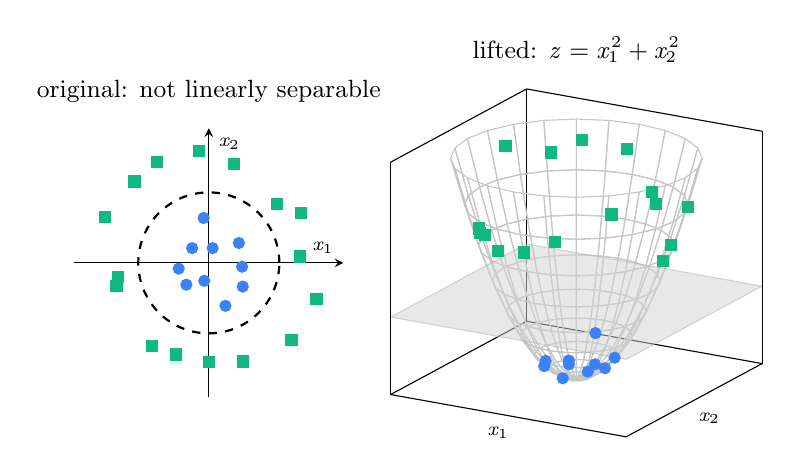
\begin{tikzpicture}
  \begin{axis}[name=flat,width=5cm,height=5cm,axis equal image,xmin=-2.1,xmax=2.1,ymin=-2.1,ymax=2.1,
    axis lines=middle,ticks=none,xlabel={$x_1$},ylabel={$x_2$},label style={font=\scriptsize},
    title={original: not linearly separable},title style={font=\small},
    every axis plot/.append style={only marks,mark size=2pt}]
   \addplot[cA,mark=*] coordinates {(0.52,-0.06) (0.47,0.31) (0.06,0.23) (-0.08,0.7) (-0.26,0.23) (-0.47,-0.09) (-0.35,-0.34) (-0.07,-0.28) (0.26,-0.67) (0.53,-0.37)};
   \addplot[cB,mark=square*] coordinates {(1.42,0.1) (1.44,0.78) (1.07,0.92) (0.39,1.54) (-0.15,1.74) (-0.81,1.57) (-1.16,1.27) (-1.62,0.72) (-1.42,-0.22) (-1.44,-0.36) (-0.89,-1.3) (-0.51,-1.43) (0,-1.55) (0.53,-1.54) (1.29,-1.2) (1.68,-0.56)};
   \draw[dashed,thick] (axis cs:0,0) circle[radius=1.1];
  \end{axis}
  \begin{axis}[at={(flat.east)},anchor=west,xshift=0.6cm,width=6.3cm,height=6cm,view={30}{20},
    xmin=-2,xmax=2,ymin=-2,ymax=2,zmin=0,zmax=3.6,ticks=none,
    xlabel={$x_1$},ylabel={$x_2$},label style={font=\scriptsize},
    title={lifted: $z=x_1^2+x_2^2$},title style={font=\small}]
   \addplot3[mesh,gray!45,domain=0:1.85,y domain=0:360,samples=10,samples y=25,z buffer=sort]
     ({x*cos(y)},{x*sin(y)},{x^2});
   \addplot3[surf,shader=flat,draw=gray!60,opacity=0.5,colormap={flat}{color=(gray!35) color=(gray!35)},domain=-2:2,y domain=-2:2,samples=2] {1.2};
   \addplot3[cA,only marks,mark=*,mark size=2pt] coordinates {(0.52,-0.06,0.27) (0.47,0.31,0.32) (0.06,0.23,0.06) (-0.08,0.7,0.5) (-0.26,0.23,0.12) (-0.47,-0.09,0.23) (-0.35,-0.34,0.24) (-0.07,-0.28,0.08) (0.26,-0.67,0.52) (0.53,-0.37,0.42)};
   \addplot3[cB,only marks,mark=square*,mark size=2pt] coordinates {(1.42,0.1,2.03) (1.44,0.78,2.68) (1.07,0.92,1.99) (0.39,1.54,2.52) (-0.15,1.74,3.05) (-0.81,1.57,3.12) (-1.16,1.27,2.96) (-1.62,0.72,3.14) (-1.42,-0.22,2.06) (-1.44,-0.36,2.2) (-0.89,-1.3,2.48) (-0.51,-1.43,2.3) (0,-1.55,2.4) (0.53,-1.54,2.65) (1.29,-1.2,3.1) (1.68,-0.56,3.14)};
  \end{axis}
  \end{tikzpicture}
  \caption{Lifting in 2D: with $\varphi(\vect x)=(x_1,\,x_2,\,x_1^2+x_2^2)$, the plane $z=r^2$ (third coordinate $z=x_1^2+x_2^2$, radius $r>0$) cuts the paraboloid in exactly the circle $x_1^2+x_2^2=r^2$.}
  \label{fig:lifting_2d_circle_to_plane}
\end{figure}

  \textbf{Definition:} Rewrite $F(\vect x)=\vect a^T\vect x'$ as $-F(\vect x)=\vect\theta^T\vect x$ by letting $\vect\theta$ be a lifted parameter vector ($\vect\theta=-\vect a$ under the convention below) and $\vect x$ denote the lifted feature vector $\vect x'$. Then
    \begin{eqnarray*}
      g(\vect \theta^T \vect x) &=& \frac{1}{1+e^{-\vect \theta^T \vect x}}.
    \end{eqnarray*}
\subsection{Learning in Logistic Regression}\label{sec:lr_learning}
Here we describe how the learning happens during logistic regression. 

\subsubsection{Log-Likelihood Function}
   \begin{itemize}
    \item Label coding in this section: $y\in\{0,1\}$.
    \item Let us assume the posteriors are given by
      \begin{eqnarray*}
        p(y=0\mid\vect x;\vect\theta) &=&  1-g(\vect \theta^T\vect x) \\
        p(y=1\mid\vect x;\vect\theta) &=&  g(\vect \theta^T\vect x)
      \end{eqnarray*}
      where $g(\vect \theta^T\vect x)$ is the sigmoid function parameterized by $\vect \theta$. 
      \textbf{Note:} Chapter 03 wrote $p(y=0\mid\vect x)=g(F(\vect x))$. Here the sigmoid models class $y=1$, i.\,e.\ $\vect\theta^T\vect x=-F(\vect x)$.
    \item The parameter vector $\vect{\theta}$ has to be estimated from a set $S$ of $m$ training samples:
      \begin{displaymath}
        S = \{(\vect x_i, y_i)\}_{i=1}^m\,.
      \end{displaymath}
    \item Method of choice: \textbf{Maximum Likelihood Estimation}
  \end{itemize}

Before we work on the formulas of the ML-estimator, we rewrite the posteriors using a \textbf{Bernoulli} model (requires $y\in\{0,1\}$):
  \begin{eqnarray*}
    p(y\mid\vect x;\vect\theta) &=&  g(\vect \theta^T\vect x)^{y}\big(1-g(\vect \theta^T\vect x)\big)^{1-y}
  \end{eqnarray*}
  The likelihood for independent samples is $\prod_{i=1}^m p(y_i\mid\vect x_i;\vect\theta)$, and thus the log-likelihood is
 
  \begin{eqnarray*}
    \mathcal{L} (\vect \theta) &=& \log \left( \prod_{i=1}^m p(y_i\mid\vect x_i;\vect\theta) \right) \\     &=& \sum_{i=1}^m \log \left( g(\vect \theta^T\vect x_i)^{y_i}\,\big(1-g(\vect \theta^T\vect x_i)\big)^{1-y_i} \right) \\ 
                              &=& \sum_{i=1}^m \left(y_i \log g(\vect \theta^T\vect x_i) + (1-y_i)\log\big(1-g(\vect \theta^T\vect x_i)\big) \right)
  \end{eqnarray*}
  Simplification of the log-likelihood function:
 
  \begin{eqnarray*}
    \mathcal{L} (\vect \theta)
      &=& \sum_{i=1}^m \left( y_i \log g(\vect \theta^T\vect x_i) + (1-y_i)\log\big(1-g(\vect \theta^T\vect x_i)\big) \right) \\
      &=& \sum_{i=1}^m \left( y_i \log \frac{e^{\vect \theta^T \vect x_i}}{1 + e^{\vect \theta^T \vect x_i}} + (1 - y_i) \log \frac{1}{1 + e^{\vect \theta^T \vect x_i}} \right) \\
      &=& \sum_{i=1}^m \left( y_i \vect \theta^T \vect x_i + \log \frac{1}{1 + e^{\vect \theta^T \vect x_i}} \right) \\
      &=& \sum_{i=1}^m \left( y_i \vect \theta^T \vect x_i + \log \big( 1 - g(\vect \theta^T \vect x_i) \big) \right)
  \end{eqnarray*}

  The ML estimate is
  \begin{displaymath}
    \hat{\vect\theta} = \argmax_{\vect\theta}\mathcal{L}(\vect\theta)\,.
  \end{displaymath}

  \textbf{Notes for the expert:} 

  \begin{itemize}
    \item The negative of the log-likelihood function is the cross entropy of
      $y$ and $g(\vect \theta^T\vect x)$. 
    \item The negative of the log-likelihood function is a convex function. Convexity is important to be able to optimize the log likelihood function and find the optimal value. 
  \end{itemize}
  
  \subsubsection{Newton-Raphson Iteration}
  
  In numerical analysis, Newton's method, also known as the Newton–Raphson method,is a root-finding algorithm which produces successively better approximations to the roots (zeros) of a real-valued function. Applied to the \emph{gradient} of the log-likelihood, it finds a stationary point; since the log-likelihood is concave, this stationary point is the maximum, i.\,e.\ the ML estimate. \footnote{https://en.wikipedia.org/wiki/Newton\%27s\_method}
 Maximization of the log-likelihood function -
   \begin{itemize}
    \item The log-likelihood function is concave.
    \item We use the \href{http://www.stat.washington.edu/quinn/classes/560/Newton.pdf}{\textbf{Newton--Raphson}} algorithm to solve the unconstrained optimization problem:
    
      For the $(k+1)$-st iteration step, we get:
%
      \begin{eqnarray*}
        \vect \theta^{(k+1)} &=& \vect \theta^{(k)} - \left(  \frac{\partial^2}{\partial\vect \theta \partial \vect \theta^T} \mathcal{L} \left(\vect \theta^{(k)} \right)  \right)^{-1}   
       \frac{\partial}{\partial\vect \theta} \mathcal{L}\left(\vect \theta^{(k)}\right)
      \end{eqnarray*}
  \end{itemize}
  \textbf{Note:} If you write the Newton-Raphson iteration in matrix form, you will end up with a weighted least squares iteration scheme.

  \textbf{Taylor's Theorem:} Approximation of an $n$-times differentiable function $f(x)$ around a given point $x_0$ (here $x$ is a scalar variable):
   {\small
  \begin{displaymath}
    f(x_0+h) = f(x_0) + f'(x_0) h + \frac{f''(x_0)}{2!} h^2 + \ldots +
           \frac{f^{(n)}(x_0)}{n!} h^n + r_n(x_0 + h) h^n, 
           \quad \lim_{h \rightarrow 0} r_n(x_0 + h) = 0
  \end{displaymath}
  }
  \textbf{Second order Taylor polynomial:}
  \begin{displaymath}
    f(x_0 + h) \approx f(x_0) + f'(x_0) h + \frac{1}{2} f''(x_0) h^2
  \end{displaymath}
\textbf{Extremum:}
  \begin{eqnarray*}
    f'(x_0 + h)         & \approx & f'(x_0) + f''(x_0) h ~\stackrel{!}{=}~ 0 \\[.3cm]
                \hat{h} & = & - \frac{f'(x_0)}{f''(x_0)} \\[.3cm]
    x_1 = x_0 + \hat{h} & = & x_0 - \frac{f'(x_0)}{f''(x_0)} 
  \end{eqnarray*}
  \textbf{Gradient of the Log-Likelihood Function}
  \noindent Let $\theta_j$ denote the $j$-th component of $\vect\theta$.
 %
  {\small
  \begin{eqnarray*}
    \frac{\partial}{\partial \theta_j} \mathcal{L}(\vect \theta)
      &=& \frac{\partial}{\partial \theta_j} \left( \sum_{i=1}^m \left( y_i \vect \theta^T \vect x_i + \log \big( 1 - g(\vect \theta^T \vect x_i) \big) \right) \right)\\ 
      &=& \sum_{i=1}^m \left( y_i x_{i,j} - \frac{1}{1-g(\vect \theta^T\vect x_i)} \frac{\partial}{\partial \theta_j}g(\vect \theta^T \vect x_i) \right)
  \end{eqnarray*}
  }
   {\small
  \begin{eqnarray*}
     \frac{\partial}{\partial \theta_j} \mathcal{L}(\vect \theta) 
       &=& \sum_{i=1}^m \left( y_i x_{i,j} - \frac{1}{1-g(\vect \theta^T\vect x_i)} g(\vect \theta^T \vect x_i) \big(1-g(\vect \theta^T \vect x_i)\big) x_{i,j} \right) \\ 
       &=& \sum_{i=1}^m \left( y_i - g(\vect \theta^T\vect x_i) \right) x_{i,j}
  \end{eqnarray*}
  } 
   Finally, we have a quite simple gradient: 
   
  {\small
  \begin{eqnarray*}
    \frac{\partial}{\partial \theta_j} \mathcal{L}(\vect \theta) 
    &=& \sum _{i=1}^m  \left( y_i - g(\vect \theta^T\vect x_i) \right) x_{i,j}
  \end{eqnarray*}
  }
  where $x_{i,j}$ is the $j$--th component of the $i$--th training feature vector. 
  Or in vector notation:
  {\small
  \begin{eqnarray*}
    \frac{\partial}{\partial\vect \theta} \mathcal{L}(\vect \theta) 
    &=& \sum _{i=1}^m  \left( y_i-g(\vect \theta^T\vect x_i) \right)\vect x_{i}
  \end{eqnarray*}
  }
  \textbf{Hessian of the Log-Likelihood Function}
  \begin{itemize}
    \item The Newton--Raphson algorithm requires the Hessian matrix, i.e.\ the matrix of second derivatives with respect to the components of $\vect\theta$.
    \item Remember the derivative of the sigmoid function!
  \end{itemize}
  \begin{eqnarray*}
    \frac{\partial^2}{\partial\vect \theta \partial \vect \theta^T} \mathcal{L}(\vect \theta) &=& -
    \sum _{i=1}^m  g(\vect \theta^T\vect x_i) \left(1-g(\vect \theta^T\vect x_i)\right)\vect x_i \vect x_i^T
  \end{eqnarray*} 

  \subsection{Decision Rule}
  Given the ML estimate $\hat{\vect\theta}$, the predicted class is
  \begin{eqnarray*}
    \hat y &=& \left\{\begin{array}{ll}
      1 & \Leftrightarrow g(\hat{\vect\theta}^T\vect x) > 0.5 \Leftrightarrow \hat{\vect\theta}^T\vect x > 0 \\
      0 & \text{otherwise}
    \end{array}\right.
  \end{eqnarray*}
  The decision boundary is $\hat{\vect\theta}^T\vect x = 0$. Note that $\hat y$ is the prediction and can differ from the true label $y$ (or training labels $y_i$).

  \subsection{Perceptron and Logistic Regression}
  
  Perceptrons are explained in more detailed later in seperate chapter. 
 
  \subsection{Lessons Learned}
   \begin{itemize}
    \item Posteriors can be rewritten in terms of a logistic function.
    \item Given the decision boundary $F(\vect x)=0$, we can write down the posterior $p(y|\vect x)$ right away.
    \item Decision boundary for normally distributed feature vectors for each class is a quadratic function.
    \item If Gaussians share the same covariances, the decision boundary is a linear function.
  \end{itemize}
  
  
\subsection{Comprehensive Questions}
 \begin{itemize}
    \item How can a nonlinear function be written as a scalar product? 
    \item What is the objective function for the ML-estimation of the logistic regression parameters? 
    \item What is the difference between a gradient descent and Newton-Raphson numerical optimization scheme? 
    \item What is the parameter update rule for the logistic regression parameters using the Newton-Raphson scheme?
  \end{itemize}
  \newpage


\newpage
% !TeX root = main.tex
  
\section{Naive Bayes}

In statistics, naive Bayes classifiers are a family of simple "probabilistic classifiers" based on applying Bayes' theorem with strong (naive) independence assumptions between the features. They are among the simplest Bayesian network models, but coupled with kernel density estimation, they can achieve high accuracy levels.\footnote{\url{https://en.wikipedia.org/wiki/Naive_Bayes_classifier}} Basically assume the features are independent, for example if classifying fruits apples vs pears, we assume the size of the pear or apple is completely independent of the color, if we think of color and size as the features used in classification.\autocite{hastie2009,bishop2006}

\subsection{Independency Assumptions}

 \begin{itemize}
    \item still widely (and successfully) used 
    \item often outperforming much more advanced classifiers 
    \item appropriate in the presence of high dimensional features (curse of dimensionality). it is used to overcome the curse of dimensionality, for eg. an image will have all the pixels as the dimensions which might be 1024x1024 and that vector is too large !! 
    \item also called \textbf{''Idiot's Bayes''}
   \end{itemize}
   
   \textbf{Naive Bayes and Statistical Independency}
  
  For the class-conditional pdf $p(\vect x\mid y)$ we can do the following factorization:
%
  \begin{eqnarray*}
    p(\vect x\mid y) &=& p(x_1, x_2, \dots, x_d \mid y) \\
    &=& p(x_1\mid y)p(x_2, x_3,\dots, x_d \mid y, x_1) \\
    &=& p(x_1\mid y)p(x_2\mid y,x_1)p(x_3,x_4,\dots, x_d \mid y, x_1, x_2) \\
    &=& p(x_1\mid y)\prod_{i=2}^d p(x_i\mid y, x_1,\dots,x_{i-1})
  \end{eqnarray*} 
   \begin{itemize}
    \item The Naive Bayes classifier makes a strong \textbf{naive independence assumption}.
    \item All $d$ components $x_i$ of the feature vector $\vect x$ are assumed to be \textbf{conditionally} independent given the class $y$.
    \item This implies:
      \begin{eqnarray*}
        p(\vect x\mid y) &=& \prod_{i=1}^d p(x_i\mid y)
      \end{eqnarray*}
  \end{itemize}

  \textbf{Decision rules:}
  \begin{itemize}
    \item Bayes-optimal prediction: $\hat y^* = \argmax_y p(y\mid\vect x)$.
    \item Naive Bayes prediction (using the conditional-independence assumption):
      \begin{eqnarray*}
        \hat y &=& \argmax\limits_{y} p(y)\prod_{i=1}^d p(x_i \mid y)
      \end{eqnarray*}
      In general, $\hat y$ is only an approximation of $\hat y^*$.
  \end{itemize}

\subsection{An Example: Gaussians}
  Assume the $100$--dimensional feature vector $\vect x\in \real^{100}$ belonging to class $y$ is normally distributed and all components are {\em mutually dependent}:
 
    \begin{eqnarray*}
      \vect\mu_y &\in& \real^{100} \\
      \mat\Sigma &=&  \mat\Sigma^T \in \real^{100\times 100} 
    \end{eqnarray*}
    The total number of parameters to be estimated for each class is  $$100+100\cdot (100+1)/2= 5150.$$
 Assume the $100$--dimensional feature vector $\vect x\in \real^{100}$ belonging to class $y$ is normally distributed and all components are \textbf{mutually independent}. 
    \begin{displaymath}
      p(\vect x\mid y) = \prod_{i=1}^{100} p(x_i \mid y) \quad = \quad \prod_{i=1}^{100} \mathcal N(x_i;\mu_{y,i}, \sigma^2_{y,i}).
    \end{displaymath}
    For each component $i\in\{1,\dots,100\}$ we have to estimate mean $\mu_{y,i}\in \real$ and variance $\sigma_{y,i}^2\in \real$.
    The total number of parameters to be estimated for each class is  $$100+100= 200.$$\\
    The slides show examples of quadratic decision boundaries considering the statistical dependency and with independence assumption of the variables $x1 and x2$. 
    \textbf{Exam Notes:} Important to understand the difference clearly in these cases. \\
   Let us consider the \textbf{logit transform} for two classes $y\in\{0,1\}$:
   \begin{eqnarray*}
    \log \frac{p(y=0\mid\vect x)}{p(y=1\mid\vect x)}
      &=& \log\frac{p(y=0) p(\vect x \mid y=0)}{p(y=1) p(\vect x \mid y=1)}\\
      &=& \log\frac{p(y=0)}{p(y=1)} + \log\frac{p(\vect x \mid y=0)}{p(\vect x \mid y=1)}\\
      &=& \log\frac{p(y=0)}{p(y=1)} + \log\frac{\prod_{i=1}^d p(x_i \mid y=0)}{\prod_{i=1}^d p(x_i \mid y=1)} \\
      &=& \underbrace{f_0 + \sum_{i=1}^d f_i(x_i)}_{\mbox {\textbf{generalized additive model}}}
   \end{eqnarray*}
   with the constant $f_0=\log\frac{p(y=0)}{p(y=1)}$ and one function per feature, $f_i(x_i)=\log\frac{p(x_i\mid y=0)}{p(x_i\mid y=1)}$. This is the log-odds $F(\vect x)$ of Chapter~03. (Different symbols on purpose: in Chapter~03, $\alpha_0$ also contains the mean and covariance terms and $\alpha_i$ are constant coefficients.)
   Understand the difference between Naive Bayes and Bayes. There are multiple techniques to beat the curse of dimensionality, for example:
   \begin{itemize}
     \item Reduction of the parameter space
       \begin{itemize}
         \item Introduction of independency assumptions
           (from complete dependency to mutual independency)
         \item Parameter tying
       \end{itemize}
    \item Reduction of the dimension of the feature vectors       
  \end{itemize}
   First order dependency
  \begin{eqnarray*}
    p(\vect x\mid y) &=& p(x_1, x_2, \dots, x_d \mid y) \\
                 &=& p(x_1\mid y)p(x_2, x_3,\dots, x_d \mid y, x_1) \\
                 &=& p(x_1\mid y)p(x_2\mid y,x_1)p(x_3,x_4,\dots, x_d \mid y, x_1, x_2) \\
                 &=& p(x_1\mid y)\prod_{i=2}^d p(x_i\mid y, x_1,\dots,x_{i-1}) \\
                 &\approx& p(x_1\mid y)\prod_{i=2}^d p(x_i\mid y, x_{i-1})
  \end{eqnarray*}
  where the last step is the first-order dependency assumption $p(x_i\mid y,x_1,\dots,x_{i-1})\approx p(x_i\mid y,x_{i-1})$.
  Example:
    \textbf{First order dependency} in a Gaussian random vector corresponds to a tridiagonal structure in the \textbf{inverse covariance (precision) matrix} $\mat Q = \mat\Sigma^{-1}$ (in general $\mat\Sigma$ itself is dense):

    \begin{eqnarray*}
      \mat Q &=& \left(
        \begin{array}{ccccccc}
          q_{1,1} & q_{2,1} & 0            & 0            & \cdots & 0              & 0 \\
          q_{2,1} & q_{2,2} & q_{3,2} & 0            & \cdots & 0              & 0 \\
          0            & q_{3,2} & q_{3,3} & q_{4,3} & \cdots & 0              & 0 \\
          0            & 0            & q_{4,3} & q_{4,4} & \cdots & 0              & 0 \\
          \vdots       & \vdots       & \vdots       & \vdots       & \ddots & \vdots         & q_{d,d-1} \\
          0            & 0            & 0            & 0            & \cdots & q_{d,d-1} & q_{d,d} \\
        \end{array}
      \right)
    \end{eqnarray*}
    Example: first-order dependency with \textbf{tied diagonal elements}, i.\,e.\ $q_{i,i}=q$:
      \begin{eqnarray*}
     \mat Q &=& \left(
       \begin{array}{ccccccc}
         q       & q_{2,1} & 0            & 0            & \cdots & 0              & 0 \\
         q_{2,1} & q       & q_{3,2} & 0            & \cdots & 0              & 0 \\
         0            & q_{3,2} & q       & q_{4,3} & \cdots & 0              & 0 \\
         0            & 0            & q_{4,3} & q       & \cdots & 0              & 0 \\
         \vdots       & \vdots       & \vdots       & \vdots       & \ddots & \vdots         & q_{d,d-1} \\
         0            & 0            & 0            & 0            & \cdots & q_{d,d-1} & q \\
       \end{array}
     \right)
    \end{eqnarray*}
    
    \subsection{Lessons Learned}
\begin{itemize}
    \item Na{\"i}ve Bayes is rather successful. 
    \item Na{\"i}ve Bayes does not require a huge set of training data. 
    \item Statistical dependency vs. dimension of the search space. 
    \item Na{\"i}ve Bayes: give it a try!
  \end{itemize}

\subsection{Comprehensive Questions}
 \begin{itemize}
    \item What is the assumption of Naive Bayes? 
    \item How does the assumption affect the class-conditional pdf $p(\vect x\mid y)$? 
    \item What is the structure of the covariance matrix of normal-distributed classes in Naive Bayes? 
    \item How can Naive Bayes be extended to first-order statistical dependencies?
  \end{itemize}
  \newpage

\section{Discriminative Analysis}

 \textbf{Discriminant analysis} methods are \textbf{generative modeling} methods: they model the prior $p(y)$ and the class-conditional density $p(\vect x\mid y)$ and obtain the posterior through Bayes' rule.\autocite{hastie2009,bishop2006}
  
  \begin{displaymath}
    p(y\mid\vect x) = \frac{p(y)\cdot p(\vect x\mid y)}{\sum_{y'} p(y')\cdot p(\vect x\mid y')}
  \end{displaymath}
  LDA is a generative method despite its name, since it models the joint probability of the data and class.\footnote{https://stats.stackexchange.com/questions/411824/linear-discriminant-analysis-generative-or-discriminative}
  
  \subsection{Gaussian Classifier}
   We call the Bayesian classifier \textbf{Gaussian}, if the class conditional density $p(\vect x|y)$ is Gaussian,(for eg. the availability of apples is gaussian in nature throughout the year) i.\,e.

  \begin{eqnarray*}
     p(\vect x | y) &=& \mathcal {N} (\vect x ;\vect {\mu}_y, \mat\Sigma_y) \\
                   &=& \frac{1}{\sqrt{\det 2\pi  \mat\Sigma_y}} 
                       e^{-\frac{1}{2}(\vect x -\vect{\mu}_y)^T \mat\Sigma_y^{-1}(\vect x - \vect{\mu}_y)}
  \end{eqnarray*}
  %
  where
%
  \begin{center}
    \begin{minipage}{0.6\textwidth}
      \begin{itemize}
        \item[$\vect x \in \real^d$:] $d$-dimensional feature vector\\
        \item[$\vect {\mu}_y \in \real^d $:] mean vector of class y\\
        \item[$ \mat\Sigma_y \in \real^{d\times d}$:] positive definite covariance matrix.
      \end{itemize}
    \end{minipage}
  \end{center}
  
  \textbf{Facts about Gaussian classifiers:}

  \begin{itemize}
    \item In general the decision boundary is \textbf{quadratic} in the components $x_j$ 
      of the feature vector $\vect x$. 
    \item If all classes share the same covariance, the decision boundary is \textbf{linear} in the components $x_j$ of the feature vector $\vect x$. 
    \item If all covariance matrices are diagonal matrices, then we get a \textbf{Naive Bayes} classifier.
    \item If all classes share the same (pooled) covariance matrix $\mat\Sigma$ and priors are identical, the optimal (Bayes) decision minimizes the \textbf{Mahalanobis distance}
      \begin{eqnarray*}
        \hat y^* &=& \argmin_{y} \frac{1}{2} (\vect x-\vect\mu_y)^T\mat\Sigma^{-1}(\vect x-\vect\mu_y)
      \end{eqnarray*}
    \item If all covariance matrices are the identity matrix, we get the \textbf{nearest class mean} classifier based on the $L_2$-norm:
      \begin{eqnarray*}
        \hat y^* &=& \argmin_{y} \frac{1}{2} (\vect x-\vect\mu_y)^T(\vect x-\vect\mu_y)
      \end{eqnarray*}
      The prototype vectors are the mean vectors.
        
  \textbf{From linear to quadratic decision boundaries:} 
  A compromise between linear and quadratic decision boundaries can be achieved by using \textbf{regularized covariance matrices}:
%  
  \begin{eqnarray*}
    \mat\Sigma_y (\alpha)= \alpha \mat\Sigma_y + (1-\alpha)\mat\Sigma
  \end{eqnarray*}  
  where $\alpha\in [0,1]$ and $\mat\Sigma$ denotes the shared (pooled) covariance.  Obviously we have the extremes:
  \begin{itemize}
    \item Linear decision boundary: $\quad ~~\alpha = 0$
    \item Quadratic decision boundary: $\alpha =1$
  \end{itemize}
  \end{itemize}
  
 \subsection{Feature Transform}
  Can we find a feature transform
%  TODO fix this slide
  \begin{eqnarray*}
    \phi: \real^d &\rightarrow &\real^d
   \end{eqnarray*}
  to generate features $\phi(\vect x)$ that share the same covariance matrix?  This is how we do it -\\
   The symmetric positive definite covariance matrix $\mat\Sigma\in \real^{d\times d}$ can be decomposed using SVD (here identical to the eigen decomposition).\autocite{trefethen1997,golub1996}
%  
  \begin{eqnarray*}
    \mat\Sigma&=&  \mat{U}\mat{D}\mat{U}^T = (\mat{U}\mat{D}^{\frac{1}{2}})(\mat{U}\mat{D}^{\frac{1}{2}})^T  =      (\mat{U}\mat{D}^{\frac{1}{2}})\cdot \mat{I} \cdot(\mat{U}\mat{D}^{\frac{1}{2}})^T
  \end{eqnarray*}
  where $\mat{I}\in \real^{d\times d}$ is the identity matrix.
 
  \begin{itemize}
    \item \textbf{Determinant:}  
      \begin{displaymath}
        \det \mat\Sigma = \prod_{i=1}^d \lambda_i,
      \end{displaymath}
      where $\mat D=\mathrm{diag}(\lambda_1,\dots,\lambda_d)$ and $\lambda_i>0$ are the \textbf{eigenvalues} (= singular values) of $\mat\Sigma$.
    \item \textbf{Inverse:}
      \begin{displaymath}
        \mat\Sigma^{-1} = \mat{U}\mat{D}^{-1}\mat{U}^T
                          = (\mat{U}\mat{D}^{-\frac{1}{2}})\cdot \mat{I} \cdot(\mat{U}\mat{D}^{-\frac{1}{2}})^T
      \end{displaymath}
  \end{itemize}
     Now we incorporate this:
   
  \begin{eqnarray*}
    \mathcal {N} (\vect x ;\vect {\mu}, \mat\Sigma) 
      &=& \frac{1}{\sqrt{\det 2\pi  \mat\Sigma}} 
          e^{-\frac{1}{2}(\vect x -\vect{\mu})^T \, \mat\Sigma^{-1} \, (\vect x - \vect{\mu})} \\
      &=& \frac{1}{\sqrt{\det 2\pi  \mat\Sigma}} 
          e^{-\frac{1}{2}(\vect x -\vect{\mu})^T \, (\mat{U}\mat{D}^{-\frac{1}{2}})\cdot \mat{I} \cdot(\mat{U}\mat{D}^{-\frac{1}{2}})^T \, (\vect x - \vect{\mu})} \\
      &=& \frac{1}{\sqrt{\det 2\pi  \mat\Sigma}} 
          e^{-\frac{1}{2} \big( (\mat{D}^{-\frac{1}{2}}\mat{U}^T)\vect x - (\mat{D}^{-\frac{1}{2}}\mat{U}^T)\vect\mu \big)^T \,\mat{I} ~
          \big( (\mat{D}^{-\frac{1}{2}}\mat{U}^T)\vect x- (\mat{D}^{-\frac{1}{2}}\mat{U}^T)\vect\mu \big) }
  \end{eqnarray*}
  The classwise transform $\phi_y$ is even a linear function:
%
  \begin{displaymath}
    \vect x' \quad = \quad \phi_y(\vect x) \quad = \quad \mat{D}_y^{-\frac{1}{2}}\mat{U}^T_y\vect x
  \end{displaymath}
  It is straight forward  to show that $\vect x'$ is normally distributed
  \begin{displaymath}
     p(\vect x' | y) \quad = \quad \mathcal {N} (\vect x' ; \vect {\mu}'_y, \mat\Sigma'_y) 
                    \quad = \quad \mathcal {N} (\vect x' ; \mat{D}_y^{-\frac{1}{2}}\mat{U}^T_y\vect {\mu}_y, \mat{I}) 
  \end{displaymath}
   \textbf{Conclusions:}
  
  \begin{itemize}
    \item All classes $y$ share the same covariance matrix that is the identity matrix.
    \item With class-specific transforms $\phi_y$, the boundary in the original feature space is still in general \emph{quadratic}; it becomes linear (a \emph{hyperplane}) only in the transformed space for each fixed $y$.
    \item \textbf{Huge disadvantage:} feature transform depends on the class index $y$ (class-specific transform $\phi_y$). This is undesirable: for large data sets we would need to estimate and apply a separate transform for each class.
    \item If we have a classified training set, we can compute a transform for each class such that all covariance matrices are the identity matrix.
    \item Classification requires the application of different transforms.
  \end{itemize}
  
  \subsection{Linear Discriminant Analysis}
  
  A method to do the feature transform that is common for all samples. The idea is similar to before and the steps to do the actual feature transform is shared here. Note: need to understand linear algebra fundamentals on what is SVD, many resources available online. LDA is a generative method, despite its name.\footnote{\url{https://towardsdatascience.com/fishers-linear-discriminant-intuitively-explained-52a1ba79e1bb}} LDA is built on Fishers discriminant analysis which is explained later.\footnote{\url{https://www.geeksforgeeks.org/ml-linear-discriminant-analysis/}}\footnote{\url{https://en.wikipedia.org/wiki/Linear_discriminant_analysis}}
  
   \begin{algorithmic}
    \STATE \textbf{Input:} training data:  $S = \{ (\vect x_1, y_1), (\vect x_2, y_2), (\vect x_3, y_3), \dots, (\vect x_m, y_m) \}$\\
    \STATE 1. ML estimation of the \textbf{class means} and the \textbf{shared (pooled) covariance matrix}:
      \begin{displaymath}
        \hat{\vect\mu}_y = \frac{1}{m_y}\sum_{i:\,y_i=y} \vect x_i, \qquad
        \widehat{\mat\Sigma}= \frac{1}{m} \sum_{i=1}^m (\vect x_i - \hat{\vect \mu}_{y_i})(\vect x_i - \hat{\vect \mu}_{y_i})^T
      \end{displaymath}
      where $m_y = |\{i: y_i=y\}|$ is the number of training samples of class $y$.
     \STATE 2. Compute SVD of the estimated covariance matrix: $\widehat{\mat \Sigma}= \mat{U}\mat{D}\mat{U}^T$ 
     \STATE 3. Assign transform: 
       \begin{displaymath}
         \phi(\vect x)= \mat D^{-\frac{1}{2}} \mat{U}^T\vect x
       \end{displaymath}
     \STATE 4. Compute transformed mean vectors for all $y$
       \begin{displaymath}
          \vect{\mu}'_y = \phi(\hat{\vect\mu}_y)= \mat{D}^{-\frac{1}{2}} \mat{U}^T \hat{\vect{\mu}}_y
       \end{displaymath}
     \STATE \textbf{Output:} feature transform $\phi$, transformed mean vectors $\vect{\mu}'_y$
  \end{algorithmic}
   Decision rule using \textbf{sphered data $\phi(\vect x)$}: the predicted label $\hat y$ of a feature vector $\vect x$ is
  \begin{eqnarray*}
    \hat y &=&  \argmax_y p(y\mid \phi(\vect x))\\ 
        &=& \argmax_y 
              \left\{ 
                \log p(y) - \frac{1}{2} \big( \phi(\vect x) - \phi(\hat{\vect\mu}_y) \big)^T \big( \phi(\vect x)-\phi(\hat{\vect\mu}_y) \big)
              \right\} \\ 
        &=& \argmin_y \left\{ \frac{1}{2}\left\|\phi(\vect x)-\phi(\hat{\vect\mu}_y) \right\|_2^2 - \log p(y) \right\}
  \end{eqnarray*}
  where $\|.\|_2$ denotes the $L_2$ norm and the class means are replaced by their estimates $\hat{\vect\mu}_y$.\\
  (Plug-in classifier: $\hat y$ approximates the Bayes decision $\hat y^*$.)\\[0.3cm]
  
  \textbf{Conclusions:}\\
  \begin{itemize}
    \item If all classes share the \textbf{same prior},  the decision rule is the \textbf{nearest class mean} decision rule, where transformed mean vectors serve as prototypes.
    protoypes : refer to the mean of the clusters, could be scalar or vector depending on the samples x.
    \item The feature transform $\phi$ does not change the dimension of features.
  \end{itemize}
   \textbf{2 classes} $y\in\{0,1\}$: insights from geometrical analysis of sphered data. the most common case is to have only two classes, so throughout the document, we focus on 2 class cases. It is clear from the slides, that in the 2 class case, the angle can tell us if the sample belongs to one class or the other. so just 1D information can seperate the samples in a 2 class case. 
   
  \begin{itemize}
    \item Angle between $\phi(\vect x)$ and $(\phi(\hat{\vect \mu}_1)-\phi(\hat{\vect \mu}_0))$ can be used 
      for decision making.
    \item Decision rule (equal priors):
      {\small
      \begin{displaymath}
        \hat y = \left\{
                \begin{array}{cl}
                  0, & \quad \mbox{if} \quad 
                       \phi(\vect x)^T \big( \phi(\hat{\vect\mu}_1) - \phi(\hat{\vect\mu}_0) \big) < 
                       \frac{1}{2} \big( 
                         \phi(\hat{\vect{\mu}}_1)^T \phi(\hat{\vect{\mu}}_1) - 
                         \phi(\hat{\vect{\mu}}_0)^T \phi(\hat{\vect{\mu}}_0) 
                        \big) \\
%                       \big( \phi(\vect{\mu}_1) + \phi(\vect{\mu}_0) \big)^T
%                       \big( \phi(\vect{\mu}_1) - \phi(\vect{\mu}_0) \big) \\[.3cm]
                  1, & \quad \mbox{otherwise}.
                \end{array}
              \right.
      \end{displaymath}
      }
    \item Coordinate orthogonal to the 1-D subspace spanned by $(\phi(\hat{\vect \mu}_1)-\phi(\hat{\vect \mu}_0))$ does not affect relative distances.
  \end{itemize}
    \textbf{$K$ classes:} insights from geometrical analysis of sphered data. This is the multi-class case, better to understand as well. naturally derive from the previous case. in a $(K)$ class case, a $(K-1)$ dimension subspace can separate the samples between the $(K)$ classes. any other information is extra and not needed. 
  \begin{itemize}
    \item Class centroids span $(K-1)$-dimensional subspace. 
    \item Relative differences are not affected by coordinates in the $(d-K+1)$-dimensional subspace that is orthogonal to the  $(K-1)$-dimensional subspace spanned by class centroids.
  \end{itemize}
    \textbf{Objective:} \\
  Will we gain an advantage if we transform features by $$\phi: \real^d\rightarrow \real^k$$ in higher $(k>d)$ or lower dimensional $(k<d)$ spaces? This is something to think about and explored in detail in the next chapters. 
  
  \subsection{Lessons Learned}
\begin{itemize}
    \item Relationship between Bayesian classifier, Gaussian classifier, and nearest class mean classifier. 
    \item Mahalanobis distance 
    \item Linear Discriminant Analysis is a regularized nearest class mean classifier 
    \item Class centroids span $(K-1)$-dimensional subspace 
  \end{itemize}
  
  \subsection{Comprehensive Questions}
  \begin{itemize}
    \item What is a Gaussian classifier? 
    \item What is the idea behind the feature transform for the LDA? 
    \item Formulate the LDA for normally distributed classes. 
    \item What is the dimensionality of the LDA subspace for $K$ classes?
  \end{itemize}
  
  \subsection{Rank Reduced Linear Discriminant Analysis}

In this section we explore what happens when further reducing the dimensions and using LDA. previously we spoke about how $(K-1)$ dimension sub-space is sufficient to distinguish between $(K)$ classes, so make that $L$ now. as explained in the video, we want to maximize the spread of this $L$ dim sub-space. it means when we project this large N dim features to $L$ dim sub-space , it should retain the max information. This can be done using PCA, since that is what PCA does. \\
Note: refer to the intro to PR classes for PCA or many resources available online. 

\begin{center}
		\begin{minipage}{0.8\textwidth}
			\begin{itemize}
				\item[{\bf Problem}:] How to choose an $L$-dimensional subspace with $L\le K-1$ that is good for  LDA? 
				\item[{\bf Idea}:] Maximize the spread of the $L$-dimensional projection of centroids. 
				\item[{\bf Solution}:] Principal component analysis, i.\,e.\    we compute the principal components of the  covariance matrix of the mean vectors
				      $$\vect{\mu}'_y = \phi(\hat{\vect{\mu}}_y) \in \real^{d},$$
				      where $y=1,2,\dots, K$ and $\phi:\real^d\to\real^d$.
			\end{itemize}
		\end{minipage}
	\end{center}
		In \textbf{Principal Component Analysis (PCA)} we compute a linear mapping $\mat\Phi \in \real^{L \times d}$ that
	results in the highest spread of projected features:
	
	\begin{displaymath}
		\mat{\Phi}^* = \argmax_{\mat{\Phi}} \left(
		\frac{1}{K}
		\sum_{y=1}^K (\mat{\Phi}\vect {\mu}'_y - \mat {\Phi}\bar{\vect \mu}' )^T
		(\mat{\Phi}\vect {\mu}'_y - \mat {\Phi}\bar{\vect \mu}' ) +
		\sum_{i=1}^{L} \nu_i (\| \mat{\Phi}_i \|_2^2 - 1)
		\right)
	\end{displaymath}
	where we applied the \textbf{Lagrange multiplier} method to allow for the maximization of the spread subject to
	\begin{displaymath}
		\| \mat {\Phi}_i \|_2^2 = 1 ~, \quad i = 1, \ldots, L ~.
	\end{displaymath}	%
	Here $\| \mat{\Phi}_i \|_2^2$ denotes the squared $L_2$ norm of the $i$-th row vector of $\mat{\Phi}$, \\
	$\nu_i$ are the Lagrange multipliers, and $\bar{\vect\mu}' = \frac{1}{K}\sum_{y=1}^K\vect\mu'_y$.\\
	Note: the derivation is not straight fwd. look at intro to PR to understand the derivation. have to use fundamentals of linear algebra approach. derivation is not important for exam. 
	
	\subsection{Excursus: Optimization with Constraints}
	very brief explanation of lagrangian constraints and optimization. it is a method to find the max value that satisfies a condition relationship like below. Lagrangians is covered in more detail in optimization chapter. or look online for more resources. 
	
		\begin{itemize}
			\item Find the maximum of $f(x,y) = x +y$ 
			\item constraint: $x^2 + y^2 = 1$ 
			\item Lagrange function: \\
			      $\mathcal L(x,y,\nu) = x + y + \nu(x^2 + y^2 - 1)$ 
			\item Set the partial derivatives to zero: \\
			      $\frac{\partial \mathcal L}{\partial x} =
				      \frac{\partial \mathcal L}{\partial y} =
				      \frac{\partial \mathcal L}{\partial \nu}
				      \stackrel{!}{=} 0$
		\end{itemize}
	We need some facts from matrix calculus: 	\footnote{www.matrixcookbook.com} \footnote{website currently offline-you can still download it at \url{http://www2.imm.dtu.dk/pubdb/views/publication_details.php?id=3274} } 
	
	\begin{enumerate}
		\item Let $\vect\mu$ denote the mean and $\mat \Sigma$ the covariance matrix of a random vector $\vect x$, then we get:
		      \begin{displaymath}
			      E[(\mat A \vect x)^T(\mat A \vect x)] =
			      {\mbox{tr}}(\mat A \mat \Sigma \mat A^T) + (\mat A \vect \mu)^T(\mat A\vect \mu)
		      \end{displaymath}
		\item The matrix derivative is:
		      \begin{displaymath}
			      \frac{\partial \mbox{tr}( \mat X \mat B \mat X^T)}{\partial \mat X} = \mat X\mat B^T +\mat X\mat B
		      \end{displaymath}
	\end{enumerate}
For our \textbf{optimization problem} this implies:

	\begin{eqnarray*}
		& & \frac{\partial}{\partial{\mat{\Phi}}}
		\left\{
		\frac{1}{K} \sum_{y=1}^K (\mat{\Phi} \vect{\mu}'_y - \mat{\Phi} \bar{\vect{\mu}}' )^T
		(\mat{\Phi} \vect{\mu}'_y - \mat{\Phi} \bar{\vect{\mu}}' )  +
		\sum_{i=1}^{L} \nu_i (\| \mat{\Phi}_i \|^2_2 - 1)
		\right\} \\
		& & = \quad \frac{\partial}{\partial{\mat{\Phi}}}
		\left\{
		\frac{1}{K} \sum_{y=1}^K \left( \mat\Phi (\vect{\mu}'_y - \bar{\vect{\mu}}') \right)^T
		\left( \mat\Phi (\vect{\mu}'_y - \bar{\vect{\mu}}') \right) +
		\sum_{i=1}^{L} \nu_i (\| \mat {\Phi}_i \|^2_2 - 1)
		\right\} \\
		& & = \quad \frac{\partial}{\partial{\mat{\Phi}}}
		\left\{
		\mbox{tr} (\mat\Phi \ \mat \Sigma_{\mbox{inter}} \ \mat\Phi^T) +
		\sum_{i=1}^{L} \nu_i (\| \mat {\Phi}_i \|_2^2 - 1)
		\right\}
		\stackrel{!}{=} \mat 0,
	\end{eqnarray*}
	{\small where $\mat \Sigma_{\mbox{inter}} = \frac{1}{K}\sum_{y=1}^K (\vect \mu'_y - \bar{\vect \mu}')(\vect \mu'_y - \bar{\vect \mu}')^T$ is the inter-class (between-class) covariance matrix of the transformed class means.}
Now we compute the \textbf{partial derivatives}:

	\begin{displaymath}
		\frac{\partial}{\partial{\mat{\Phi}}}
		\left\{
		\mbox{tr} (\mat \Phi \ \mat \Sigma_{\mbox{inter}}  \ \mat \Phi^T) + \sum_{i=1}^{L} \nu_i (\| \mat {\Phi}_i \|^2_2 - 1)  \right\} =
		2 \mat \Phi\mat  \Sigma_{\mbox{inter}} +2 \mat{\Nu} \mat \Phi = \mat 0,
	\end{displaymath}
	where $\mat\Nu = \mbox{diag}(\nu_1,\dots,\nu_L)$ contains the Lagrange multipliers.
	This results in the eigenvalue and eigenvector problem:
	\begin{displaymath}
		\mat{\Sigma}_{\mbox{inter}} \mat \Phi^T = \mat \Phi^T \mat{\Lambda}', \qquad \mat\Lambda' = -\mat\Nu = \mbox{diag}(\lambda'_1,\dots,\lambda'_L),
	\end{displaymath} 
	i.\,e.\ the rows of $\mat\Phi$ are eigenvectors of $\mat\Sigma_{\mbox{inter}}$ with eigenvalues $\lambda'_i$.
	\textbf{Note:} \\
	In original PCA, the transform $\mat \Phi$ maximizes the overall spread using the covariance matrix of all features:
	\begin{displaymath}
		\mat{\Sigma}\,\mat{\Phi}^T = \mat{\Phi}^T\,\mat{\Lambda}',
	\end{displaymath}
	\begin{algorithmic}
		\STATE  \textbf{Input:} training data:  $S = \{ (\vect x_1, y_1), (\vect x_2, y_2), (\vect x_3, y_3), \dots, (\vect x_m, y_m) \}$ \\
		\STATE 1. Compute the covariance matrix of transformed mean vectors
		$$\widehat{\mat{\Sigma}}_{\mbox{inter}} =
			\frac{1}{K} \sum_{y=1}^K (\vect \mu'_y - \bar{\vect \mu}')(\vect \mu'_y - \bar{\vect \mu}')^T,$$
		\quad\,where $\bar{\vect \mu}' = \frac{1}{K} \cdot \sum_{y=1}^{K}\vect\mu'_y$. \\
		\STATE 2. Compute the $L$ eigenvectors of the covariance matrix belonging \\
		\quad\,to the largest eigenvalues. \\
		\STATE 3. The eigenvectors are the rows of the mapping $\mat\Phi\in\real^{L\times d}$.
		\quad\,(The class centroids span at most a $(K-1)$-dimensional subspace of $\real^d$.) \\
		\STATE  \textbf{Output:} matrix $\mat\Phi$
	\end{algorithmic}
	
	\subsection{Fisher Transform}%
	References to read are given below \footnote{\url{https://www.stat.cmu.edu/~ryantibs/datamining/lectures/21-clas2.pdf}}%
	\footnote{\url{https://www.cs.cmu.edu/~psarkar/sds383c_16/lecture_scribe13.pdf}}.

	The described method to compute the LDA mapping is not the original derivation. Some additional reading material.\autocite{fisher1936,bishop2006}%
	\footnote{\url{https://towardsdatascience.com/fishers-linear-discriminant-intuitively-explained-52a1ba79e1bb}}%
	\footnote{\url{https://www.ccis.northeastern.edu/home/vip/teach/MLcourse/5_features_dimensions/lecture_notes/LDA/LDA.pdf}}

\textbf{Original method}
		\begin{itemize}
			\item Project samples $\vect{x}_i$ onto a straight line with direction $\vect{r}$, $\lVert \vect{r} \rVert_2 = 1$:
			      \begin{displaymath}
				      x_i^{\mathrm{proj}} = \vect{x}_i^T \vect{r}
			      \end{displaymath}
			\item Maximize the ratio of the between-class scatter and the within-class scatter:
			      \begin{displaymath}
				      \vect{r}^* =
				      \argmax_{\vect{r}} R(\vect{r}) =
				      \argmax_{\vect{r}} \frac{|\mu_1^{\mathrm{proj}} - \mu_2^{\mathrm{proj}}|^2}{(s_1^{\mathrm{proj}})^2 + (s_2^{\mathrm{proj}})^2}
			      \end{displaymath}
			\item Classify by applying a threshold to $x_i^{\mathrm{proj}}$
		\end{itemize}
	\textbf{Finding $\vect{r}^*$}

	\begin{enumerate}
		\item Mean and scatter matrix for each class:
		      {\small
		      \begin{eqnarray*}
			      \vect{\mu}_k &=& \frac{1}{m_k} \sum_{i:\, y_i = k} \vect{x}_i \\
			      \mat{S}_k   &=& \sum_{i:\, y_i = k} (\vect{x}_i - \vect{\mu}_k) (\vect{x}_i - \vect{\mu}_k)^T
		      \end{eqnarray*}
		      }
		\item \textbf{Within-class scatter} matrix:
		      \begin{displaymath}
			      \mat{S}_{\mathsf{W}} = \mat{S}_1 + \mat{S}_2
		      \end{displaymath}
		\item \textbf{Between-class scatter} matrix:
		      \begin{displaymath}
			      \mat{S}_{\mathsf{B}} = (\vect{\mu}_1 - \vect{\mu}_2) (\vect{\mu}_1 - \vect{\mu}_2)^T
		      \end{displaymath}
	
		\item Expressing $\mu_k^{\mathrm{proj}}$ and $(s_k^{\mathrm{proj}})^2$ of the projected samples in terms of $\vect{\mu}_k$ and $\mat{S}_k$:
		      {\small
		      \begin{eqnarray*}
			          \mu_k^{\mathrm{proj}} &=&
				         \frac{1}{m_k} \sum_{i:\, y_i = k} x_i^{\mathrm{proj}} 
				       = \frac{1}{m_k} \sum_{i:\, y_i = k} \vect{r}^T  \vect{x}_i 
				       = \vect{r}^T \vect{\mu}_k  \\
				      (s_k^{\mathrm{proj}})^2 &=&
				        \sum_{i:\, y_i = k} (x_i^{\mathrm{proj}} - \mu_k^{\mathrm{proj}})^2 
				      = \sum_{i:\, y_i = k} (\vect{r}^T \vect{x}_i - \vect{r}^T \vect{\mu}_k)^2 
				      = \vect{r}^T \mat{S}_k \vect{r} 
		      \end{eqnarray*}
		      }
		\item Plug it into $R(\vect{r})$:
		      {\small
		      \begin{displaymath}
			      R(\vect{r})
			      = \frac{|\mu_1^{\mathrm{proj}} - \mu_2^{\mathrm{proj}}|^2}{(s_1^{\mathrm{proj}})^2 + (s_2^{\mathrm{proj}})^2}
			      = \frac{\vect{r}^T \mat{S}_B \vect{r}}{\vect{r}^T \mat{S}_W \vect{r}}
			      \end{displaymath}
		      }
		\item[] This is known as the \textbf{Generalized Rayleigh Quotient}.
		\item \textbf{Why this yields an eigenproblem:} since $R(\vect r)$ does not change if $\vect r$ is scaled, we can fix the denominator and solve
		      {\small
		      \[
		        \max_{\vect r}\; \vect r^T\mat S_\mathsf B\vect r
		        \quad\text{subject to}\quad \vect r^T\mat S_\mathsf W\vect r = 1~.
		      \]
		      }
		      With Lagrangian $\Lambda(\vect r,\lambda)=\vect r^T\mat S_\mathsf B\vect r-\lambda(\vect r^T\mat S_\mathsf W\vect r-1)$, stationarity gives
		      $\mat S_\mathsf B\vect r = \lambda\,\mat S_\mathsf W\vect r$.
		      Moreover, multiplying from the left by $\vect r^T$ yields $R(\vect r)=\lambda$, hence we take the generalized eigenvector with the \textbf{largest} eigenvalue.
		\item Maximizing the Generalized Rayleigh Quotient is equivalent to solving the following \textbf{generalized eigenvalue problem}:
		      {\small
		      \begin{eqnarray*}
			      \mat{S}_\mathsf{B} \vect{r}^* &=& \lambda \mat{S}_\mathsf{W} \vect{r}^* \\
			      \mat{S}_\mathsf{W}^{-1} \mat{S}_\mathsf{B} \vect{r}^* &=& \lambda \vect{r}^* \\
		      \end{eqnarray*}
		      }
		\item \textbf{Note}: $\mat{S}_\mathsf{B} \vect{r}^*$ is always in the direction of $\vect{\mu}_1 - \vect{\mu}_2$; \\
		      no need to compute the eigenvalues and eigenvectors of $\mat{S}_\mathsf{W}^{-1} \mat{S}_\mathsf{B}$! \\
		      The direction of $\vect{r}^*$ is:
		      {\small
		      \begin{displaymath}
			      \vect{r}^* = \mat{S}_\mathsf{W}^{-1} (\vect{\mu}_1 - \vect{\mu}_2)
		      \end{displaymath}
		      }	      
	\end{enumerate}
	
	\begin{itemize}
		\item Usually the total linear mapping for LDA is computed dimension by dimension through the maximization of the Rayleigh ratio for each projection axis $\vect a^*$:
		      \begin{eqnarray*}
			      \vect a^* &=& \argmax_{\vect a}\ \frac{\vect a^T \mat \Sigma_{\mbox{inter}} \vect a}{\vect a^T \mat \Sigma_{\mbox{intra}} \vect a}
		      \end{eqnarray*}
		\item The solution is a generalized eigenvalue problem: $\vect a$ is the eigenvector of
		      $$\mat \Sigma_{\mbox{intra}} ^{-1} \mat \Sigma_{\mbox{inter}}$$
		      that belongs to the largest eigenvalue.
	\end{itemize}
	In literature the optimization problem is mostly rewritten:
		\begin{itemize}
		\item Equivalent constrained optimization problem
		      \begin{eqnarray*}
			      \mbox{maximize:}   & & \vect r^T \mat \Sigma_{\mbox{inter}}\vect r\\
			      \mbox{subject to:} & & \vect r^T \mat \Sigma_{\mbox{intra}} \vect r =1
		      \end{eqnarray*}
		\item Lagrange multiplier method ($\lambda>0$):
		      \begin{displaymath}
			      \vect{r}^* = \argmax_{\vect r}
			      \left\{
			      \vect r^T \mat \Sigma_{\mbox{inter}} \vect r
			      - \lambda\big(\vect r^T \mat \Sigma_{\mbox{intra}} \vect r - 1\big)
			      \right\}
		      \end{displaymath}
	\end{itemize}

In a nutshell, we recognize the fishers problem is solved by finding the eigenvalues. 

\subsection{Dimensionality Reduction}


	A few comments on dimensionality reduction:

	\begin{itemize}
		\item PCA does not require a classified set of feature vectors  (in contrast to LDA). 
		\item PCA transformed features are approximately normally distributed (central limit theorem).
		\item Components of PCA transformed features are mutually uncorrelated. *Independent and uncorrelated if gaussian distribution. 
		\item There exist many other methods for dimensionality reduction, e.\,g.,  Sammon transform, independent component analysis. 
		\item Usually the estimation of transforms is computationally prohibited
		\item \textbf{Johnson-Lindenstrauss lemma}: If vectors are projected onto a randomly selected subspace of suitably high dimension, then the distances between the vectors are approximately preserved.
	\end{itemize}
	
\subsection{LDA application: adidas\_1 }
Refer to the slides for more detailed information. The key takeaway is to understand how a practical classification problem was solved and what was the output of using an LDA classifier. 

\subsection{PCA application: Shape Modeling}

Details in the slides, but the key takeaway is to understand how PCA is used for shape modeling. it can be easily understood that the mean of all the features represents the average shape of the organ, and PCA helps us to understand the amount of variation seen in the data. 

\subsection{Notes on Regression}
We remember that regression is basically trying to estimate a sample, not just understanding which class it belongs to. In the example of apples vs pears, we are trying to estimate the shape, size, weight of the apple using the knowledge of probabilities, prior class information about how apples are usually shaped, weigh, etc.\autocite{hastie2009,bishop2006}

\subsubsection{Linear Regression}
In the two class situation, we set $y\in \{-1,+1\}$ and use the decision rule:
	\begin{displaymath}
		\hat y = \mbox{sgn}(\vect \alpha^T\vect x + \alpha_0).
	\end{displaymath}
	We can compute the linear decision boundary simply by least-square estimation. For a given set of learning data we use matrix notation:

	\begin{displaymath}
		\mat{X} = \left(
		\begin{array}{cc}
				\vect x_1^T & 1      \\
				\vect x_2^T & 1      \\
				\vdots     & \vdots \\
				\vect x_m^T & 1
			\end{array}
		\right) \in \real^{m\times (d+1)} \qquad \vect y \quad = \quad
		\left(
		\begin{array}{c}
				y_1    \\
				y_2    \\
				\vdots \\
				y_m    \\
			\end{array}
		\right) \in \real^m
	\end{displaymath}
	and define
	\begin{displaymath}
		\vect \theta = { \vect \alpha\choose \alpha_0} \in \real^{d+1}, \qquad
		\tilde{\vect x}_i = { \vect x_i \choose 1} \in \real^{d+1}.
	\end{displaymath}
	i.\,e.\ the $i$-th row of $\mat X$ is the augmented feature vector $\tilde{\vect x}_i^T$ and $\vect\theta^T\tilde{\vect x}_i = \vect\alpha^T\vect x_i + \alpha_0$.

		One option to estimate $\vect \theta$ is to solve the linear regression problem:
	\begin{displaymath}
		\hat{\vect \theta} = \argmin_{\vect \theta}\| \mat X \vect \theta - \vect y\|_{2}^2
	\end{displaymath}
The \textbf{}{least-square estimator} for the $L_2$-norm:
	\begin{eqnarray*}
		\widehat{\vect \theta} &=& \argmin_{\vect\theta} \ \sum_{i=1}^m (\vect \theta^T\tilde{\vect x}_i-y_i)^2\\
		&=& \argmin_{\vect\theta} \ (\mat{X}\vect \theta-\vect y)^T(\mat{X}\vect \theta-\vect y)
	\end{eqnarray*}
	and thus we get
	\begin{displaymath}
		\widehat{\vect \theta} = (\mat{X}^T\mat{X})^{-1}\mat{X}^T\vect y
	\end{displaymath}
	if the column vectors of $\mat X$ are linearly independent. A few obvious questions:
	\begin{itemize}
		\item Why should we prefer the Euclidean norm ($L_2$-norm)? 
		\item Will different norms lead to different results? 
		\item Which norm and decision boundary is the best one? 
		\item Can we incorporate prior knowledge in linear regression?
	\end{itemize}	

\subsubsection{Ridge Regression}

A regression formula based on L2 norm and the regularizer is also an L2 norm. regularized expression helps to make sure, that we are always able to find the inverse. since the solution depends on finding the inverse of a matrix. \\ 

\textbf{Regularized regression:}

	\begin{eqnarray*}
		\widehat{\vect\theta}
		&=& \argmin_{\vect\theta} \| \mat{X} \vect\theta - \vect y \|^2_2 + \lambda \|\vect\theta\|^2_2 \\ 
		&=& \argmin_{\vect\theta} \ (\mat{X} \vect\theta - \vect y)^T (\mat{X} \vect\theta-\vect y) +
		\lambda \cdot \vect\theta^T\vect \theta
	\end{eqnarray*}
	and thus we get the estimator:
	\begin{displaymath}
		\widehat{\vect\theta} = (\mat{X}^T\mat{X}+\lambda \mat{I})^{-1}\mat{X}^T\vect y
	\end{displaymath}
	\textbf{Notes:}
	\begin{itemize}
		\item The term $\lambda \mat{I}$ adds a positive constant $\lambda$ to the diagonal elements.
		\item The problem is non-singular even if $\mat{X}^T \mat{X}$ is not of full rank. 
		\item This was the main motivation of ridge regression when it was first introduced in statistics in 1970.
		\item The ridge solutions are not equivariant under scaling of the inputs: 
		      \textbf{standardize} the input before solving the regression problem!  
		\item The intercept $\alpha_0$ should not be penalized, there should be bias correction which is done as shown below:
		      \begin{itemize}
			      \item \textbf{Center} the input $\vect{x}_i$.
			      \item Estimate $\alpha_0$ by $\bar{y} = \frac{1}{m} \sum_{i=1}^m y_i$.
			      \item Estimate the remaining coefficients by a ridge regression without  intercept. Matrix $\vect{X}$ has $d$ columns (instead of $d+1$).
		      \end{itemize}
	\end{itemize}
\textbf{Statistical approach:} parameters $\alpha_j$ are random variables 
	\begin{itemize}
		\item It is extended by a prior distribution on the parameter vector $\vect\theta$:
		      \begin{displaymath}
			      \vect \theta \sim {\cal N}(\vect 0, \tau^2 \mat I)
		      \end{displaymath}
		      (in practice the intercept $\alpha_0$ is excluded from the prior/penalty, see below)
		\item Suppose
		      \begin{displaymath}
			      \forall 1 \le i \le m: \quad y_i
			      \sim \mathcal{N}(\underbrace{\vect{\alpha}^T \vect{x}_i + \alpha_0}_\text{mean}, \underbrace{\sigma^2}_\text{variance})
			      ,\ \text{i.e. } p(y_i|\vect x_i,\vect\alpha) = \frac{1}{\sqrt{2 \pi} \cdot \sigma} e^{-\frac{1}{2} \cdot \frac{(y_i - \vect{\alpha}^T \vect{x}_i - \alpha_0)^2}{\sigma^2}}
  \end{displaymath}
		\item Parameters $\alpha_j$ are assumed to be independent of each other.
		\item Prior distribution of $\alpha_j$:
		      \begin{displaymath}
			      \forall 1 \le j \le d: \quad \alpha_j
			      \sim \mathcal{N}(0, \tau^2)
			      ,\ \text{i.e. } p(\alpha_j) = \frac{1}{\sqrt{2 \pi} \cdot \tau} e^{-\frac{1}{2} \cdot \frac{(\alpha_j - 0)^2}{\tau^2}}
		      \end{displaymath}
		\item {Maximizing the posterior probability of $\vect{\alpha}$ for given $\sigma^2$ and $\tau^2$:}
		      \footnotesize
		      \begin{eqnarray*}
			      \argmax_{\vect{\alpha}} p(\vect{\alpha}|S) 
			      &=& \argmax_{\vect{\alpha}} \Bigg\{ p(\vect{\alpha}) \cdot \prod_{i=1}^m p(y_i | \vect x_i, \vect{\alpha}) \Bigg\} \\ 
			      &=& \argmax_{\vect{\alpha}} \Bigg\{ \prod_{j=1}^d p(\alpha_j) \cdot \prod_{i=1}^m p(y_i | \vect x_i, \vect{\alpha}) \Bigg\} \\ 
			      &=& \argmax_{\vect{\alpha}} \Bigg\{ \sum_{j=1}^d \log p(\alpha_j) + \sum_{i=1}^m \log p(y_i | \vect x_i, \vect{\alpha}) \Bigg\} \\ 
			      &=& \argmax_{\vect{\alpha}} \Bigg\{ - \frac{1}{2 \tau^2} \sum_{j=1}^d \alpha_j^2 - \frac{1}{2 \sigma^2} \sum_{i=1}^m (y_i - \vect{\alpha}^T \vect{x}_i - \alpha_0)^2 \Bigg\} \\ 
			      &=& \argmin_{\vect{\alpha}} \Bigg\{ \frac{\sigma^2}{\tau^2} \sum_{j=1}^d \alpha_j^2 + \sum_{i=1}^m (y_i - \vect{\alpha}^T \vect{x}_i - \alpha_0)^2 \Bigg\}
		      \end{eqnarray*}
    		\item {Maximizing the posterior probability of $\vect{\alpha}$ for given $\sigma^2$ and $\tau^2$:} 
		      {\footnotesize
		      \begin{displaymath}
			      \argmax_{\vect{\alpha}} p(\vect{\alpha}|S)
			      = \argmin_{\vect{\alpha}} \Bigg\{ \lambda \vect{\alpha}^T \vect{\alpha} + (\mat{X}\vect{\theta} - \vect{y})^T (\mat{X}\vect{\theta} - \vect{y}) \Bigg\}
			      \quad \text{with} \quad
			      \lambda = \frac{\sigma^2}{\tau^2}
		      \end{displaymath}
		      where $\vect\theta = (\vect\alpha^T, \alpha_0)^T$ (the intercept $\alpha_0$ is not penalized).
		      }
		\item {The ridge estimate is the mode of the posterior pdf!}
	\end{itemize}

\subsubsection{Lasso}

A different kind of regression that is based on L1 norm regularizer. 

	Regularized regression using a mixture of $L_2$- and $L_1$-norm, where the residual is penalized using the $L_2$-norm and the regularizer uses the $L_1$-norm:

	\begin{displaymath}
		\widehat{\vect \theta} = \argmin_{\vect\theta} \|\mat{X}\vect \theta-\vect y\|^2_2 + \lambda \cdot \|\vect \theta\|_1
	\end{displaymath}
	The lasso is used to compute a sparse solution of the system of linear equations, i.\,e.\ the number of non-zero elements in $\vect \theta$ shall be small.
	
\subsection{Lessons Learned}

	\begin{itemize}
		\item Principal component analysis 
		\item Linear discriminant analysis with and without dimension reduction 
		\item Both PCA and LDA relate to an eigenvalue eigenvector problem 
		\item Alternative formulation of LDA using the Fisher transform 
		\item Linear and ridge regression for classification
	\end{itemize}
	
\subsection{Comprehensive Questions}
	\begin{itemize}
		\item What is the difference between PCA and LDA? 
		\item How can PCA and LDA be combined to achieve a high rank reduction? 
		\item Write down a straight forward objective function for linear regression! 
		\item What happens if we replace the $L_2$-norm by another norm?
	\end{itemize}
	

\newpage
% !TeX root = main.tex
\section{Norms and Norm Dependent Linear Regression}

This topic relates to optimization techniques and how to find the maxima or the minima of a curve, how to influence the selection of the parameters. for eg, when reducing the error , there could be many parameters $\vect \theta$ that satisfy an objective function. How do we decide which is the best one, or how do we influence the selection of parameters that satisfy additional criteria such as sparsity? the norms are the kinds of objective functions that force the optimizing methods to select the parameters that satisfy both the objective function and the norm criteria. It will be clearer with the next 4 chapters on optimization techniques. reading additional material is encouraged, since this forms the basis of machine learning.\footnote{\url{https://medium.com/codex/how-norms-drive-the-direction-of-your-optimization-bdbcd619256b}}
\footnote{\url{https://web.stanford.edu/~sidford/courses/20fa_opt_theory/sidford_2020fa_mse213_cs269o_lec8.pdf}}
\footnote{\url{https://utexas.instructure.com/files/43781366/download?download_frd=1}}

Sparsity constraint: we want to force as many dimensions of the parameter vector as possible to zero. 

\subsection{Motivation}

  \begin{itemize}
    \item Different norms and similarity measures play an important role in machine learning and pattern recognition. 
    \item In this chapter we summarize important definitions and facts on norms. 
    \item We consider the problem of linear regression for different norms.
    \item We will briefly look into associated optimization problems.
  \end{itemize}
  
\subsection{Notation in this Chapter}

This chapter follows the notation of numerical linear algebra and optimization (Boyd \& Vandenberghe).\autocite{boyd2004}

\begin{itemize}
  \item $\vect x$, $\vect y$ in the definitions of inner products and norms: generic vectors (not feature vectors / labels).
  \item $\mat A\in\real^{m\times d}$: data (design) matrix -- corresponds to $\mat X$ in the regression part of Chapter \emph{Discriminant Analysis II}.
  \item $\vect x$ in regression problems: unknown parameter vector (optimization variable), not a feature vector -- corresponds to $\vect\theta$.
  \item $\vect b\in\real^m$: target values -- corresponds to $\vect y$.
  \item $\hat{\vect x}$: estimate of the parameter vector, $\vect x_0$: true parameter vector.
  \item $\vect r = \mat A\vect x-\vect b$: residual vector; $\phi$: penalty function (not the LDA feature transform).
\end{itemize}

\subsection{Inner Product}

 \textbf{Definition}

The \textbf{\emph{inner product of vectors}} $\vect x, \vect y\in \real^d$ is defined by \autocite{trefethen1997,golub1996}
    \begin{displaymath}
      \langle\vect x, \vect y\rangle = \vect x^T \vect y = \sum_{i=1}^d x_iy_i \quad .
    \end{displaymath}
Example: The \textbf{\emph{Euclidean norm} ($L_2$-norm)} can be written in terms of an inner product:
    \begin{displaymath}
      \| \vect x \|_2 = \sqrt{\langle \vect x, \vect x \rangle } = 
      \sqrt{ \vect x^T \vect x} = 
      \sqrt{\sum_{i=1}^d x_i^2 }\quad .
    \end{displaymath}
\textbf{Definition}

    The \emph{inner product of matrices} $\mat X, \mat Y\in \real^{m\times n}$ is defined by 
    \begin{displaymath}
       \langle \mat X, \mat Y \rangle = 
       \mbox{tr}(\mat X^T \mat Y) = 
       \sum_{i=1}^m \sum_{j=1}^n x_{i,j} y_{i,j} \quad
    \end{displaymath}
 Example:  The \emph{Frobenius norm} can be written in terms of an inner product:
    \begin{displaymath}
      \| \mat X \|_F = 
      \sqrt{ \langle \mat X, \mat X \rangle } =
      \sqrt{ \mbox{tr}(\mat X^T \mat X)} =
      \sqrt{ \sum_{i=1}^m \sum_{j=1}^n x_{i,j}^2} \quad
    \end{displaymath}

\subsection{Norms}
 \textbf{Definition}

    The function $\lVert\cdot\rVert$ %: \real^d\rightarrow \real$ 
    is called a \textbf{\emph{norm}} if it 
   
    \begin{enumerate}
      \item is \textbf{nonnegative}: $\forall \vect x:~ \lVert\vect x\rVert\geq 0$ 
      \item is \textbf{definite}: $\|\vect x\| =0$ only if $\vect x=\vect 0$ 
      \item is \textbf{homogeneous}: $\| a\vect x\|= |a|\cdot \|\vect x\|$ where $a\in \real$ 
      \item fulfills the \textbf{triangle inequality}:
      \begin{displaymath}
        \forall \vect x, \vect y:~\|\vect x+\vect y\| \leq \|\vect x\|+ \|\vect y\|
      \end{displaymath}
    \end{enumerate}
    \begin{itemize}
      \item The \textbf{$L_0$-norm} of a $d$-dimensional vector denotes the number of    non-zero entries. Despite its name, the $L_0$-norm is not a norm because it is not homogeneous.
      \item The \textbf{$L_p$-norm} ($p \geq 1$) of a $d$-dimensional vector is defined as 
        \begin{displaymath}
          \| \vect x\|_p = \left( \sum_{i=1}^d  |x_i|^p \right)^{\frac{1}{p}}
        \end{displaymath}
    \item \textbf{$L_1$-norm:} sum of absolute values
      \begin{displaymath}
        \| \vect x\|_1 = \sum_{i=1}^d |x_i|
      \end{displaymath}
    
    \item \textbf{$L_2$-norm:} square root of the sum of squared values
      \begin{displaymath}
        \| \vect x\|_2 = \left(\sum_{i=1}^d x_i^2\right)^{\frac{1}{2}}
      \end{displaymath}
    \item \textbf{$L_\infty$-norm:} maximum norm
      \begin{displaymath}
        \| \vect x\|_\infty = 
        \lim_{p\rightarrow \infty} \left( \sum_{i=1}^d  |x_i|^p \right)^{\frac{1}{p}} =
        \max_i \{ |x_i| \ ; \ i=1,2, \dots, d \}
      \end{displaymath}
  \end{itemize}
  \textbf{Definition}
    Let $\mat P$ be a symmetric positive definite matrix.    The \emph{quadratic $L_{\mat P}$-norm} is defined by 
    \begin{displaymath}
      \| \vect x\|_{\mat P} = 
      \sqrt{ \vect x^T \mat P \vect x} = 
      \sqrt{ (\mat P^\frac{1}{2} \vect x)^T \mat P^\frac{1}{2} \vect x} =
      \| \mat P^\frac{1}{2} \vect x\|_2
    \end{displaymath}
  \textbf{Note:} 

  \begin{itemize}
    \item The $L_2$-norm is the same as the quadratic $L_{\mat I}$-norm, where $\mat I$ is the identity matrix.
    \item The \textbf{Mahalanobis distance} between two vectors $\vect x$ and $\vect y$ based on the covariance matrix $\mat \Sigma$ is given by the quadratic $L_{\mat \Sigma^{-1}}$-norm:
      \begin{displaymath}
        \| \vect x - \vect y\|_{\mat \Sigma^{-1}} = 
        \sqrt{ (\vect x - \vect y)^T \mat\Sigma^{-1} (\vect x - \vect y)}
      \end{displaymath}
    \item A norm is a measure for the length of a vector. It can also be used to measure the distance between two vectors $\vect x$ and $\vect y$:
      \begin{displaymath}
        \mbox{dist}(\vect x, \vect y) = \| \vect x - \vect y\|
      \end{displaymath}
  \end{itemize}
  \textbf{Norms of matrices} can be defined by norms of vectors.
  
  \textbf{Definition}
    \small
    Let $\|.\|_p$ and $\|.\|_q$ be norms for vectors in $\real^m$ and $\real^n$. \\
    The \textbf{\emph{operator norm}} of a matrix $\mat X\in \real^{m\times n}$  is defined by
 
    \begin{displaymath}
      \| \mat X\|_{p,q} = \sup\{ \| \mat X \vect u\|_p ; \  \| \vect u\|_q\leq 1 \}
    \end{displaymath}
  Example: If $p=q=2$, i.\,e.\ we use the $L_2$-norm twice, the operator norm of $\mat X$ results in the maximum singular value:
    
    \begin{displaymath}
      \| \mat X\|_{2,2}=   \| \mat X\|_{2} = \sigma_{\max}{(\mat X)}= \sqrt{\lambda_{\max}(\mat X^T\mat X)}
    \end{displaymath}

\subsection{Unit Balls}

The unit ball of a norm is the set of all vectors of norm at most one. Its shape (a diamond for $L_1$, a circle for $L_2$, a square for $L_\infty$ in 2-D) shows which parameter vectors a regularizer with this norm prefers; e.\,g.\ the corners of the $L_1$ ball lie on the axes, which is why the $L_1$-norm favours sparse solutions. 

  \textbf{Definition}
    The set
    \begin{displaymath}
      {\cal B} = \{ \vect x; \|\vect x\| \leq 1\}
    \end{displaymath}
    of all vectors $\vect x$ of length less or equal to one according to the norm $\|.\|$  is called the \textbf{\emph{unit ball}}.
   
 The unit balls for different norms are shown in Fig.~\ref{fig:unitballs}.
  \begin{figure}[htbp]
    \centering
    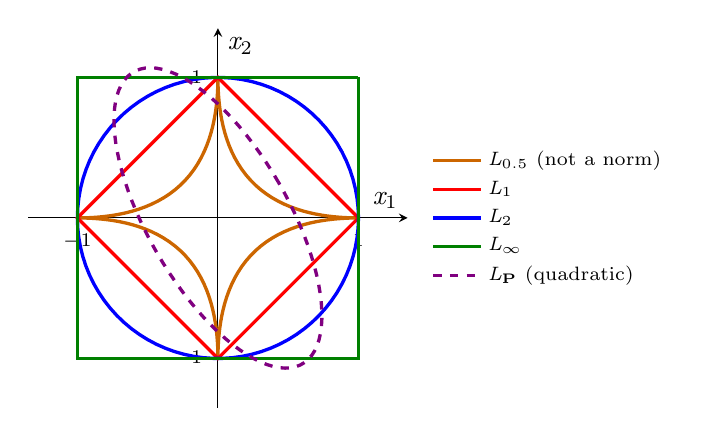
\begin{tikzpicture}
      \begin{axis}[width=6.4cm, height=6.4cm, axis equal image, axis lines=middle, xmin=-1.35, xmax=1.35, ymin=-1.35, ymax=1.35,
          xtick={-1,1}, ytick={-1,1}, tick label style={font=\scriptsize}, xlabel={$x_1$}, ylabel={$x_2$},
          legend style={font=\scriptsize, at={(1.04,0.5)}, anchor=west, draw=none}, legend cell align=left]
        \addplot[orange!80!black, very thick, domain=0:360, samples=181, variable=\t]
          ({sign(cos(\t))*abs(cos(\t))^4}, {sign(sin(\t))*abs(sin(\t))^4});
        \addlegendentry{$L_{0.5}$ (not a norm)}
        \addplot[red, very thick] coordinates {(1,0) (0,1) (-1,0) (0,-1) (1,0)};
        \addlegendentry{$L_1$}
        \addplot[blue, very thick, domain=0:360, samples=91, variable=\t] ({cos(\t)}, {sin(\t)});
        \addlegendentry{$L_2$}
        \addplot[green!50!black, very thick] coordinates {(1,1) (-1,1) (-1,-1) (1,-1) (1,1)};
        \addlegendentry{$L_\infty$}
        \addplot[violet, very thick, dashed, domain=0:360, samples=91, variable=\t]
          ({0.5*cos(\t)*cos(30)-1.2*sin(\t)*sin(30)}, {0.5*cos(\t)*sin(30)+1.2*sin(\t)*cos(30)});
        \addlegendentry{$L_{\mat P}$ (quadratic)}
      \end{axis}
    \end{tikzpicture}
    \caption{Boundaries of the unit balls $\{\vect x;\ \|\vect x\|\le1\}$ in $\real^2$: $L_1$ (diamond), $L_2$ (circle), $L_\infty$ (square), and a quadratic norm $L_{\mat P}$ (ellipse whose axes are the eigenvectors of $\mat P$, with semi-axis lengths $1/\sqrt{\lambda_i(\mat P)}$). For $p<1$ the ``ball'' $\{\vect x;\ (\sum_i|x_i|^p)^{1/p}\le1\}$ (shown for $p=0.5$) is not convex, i.\,e.\ the triangle inequality fails and $L_p$ is not a norm. For $p\ge1$ the balls are nested: $L_1\subset L_2\subset L_\infty$.}
    \label{fig:unitballs}
  \end{figure}

 \textbf{Exam notes:} It is important to know the difference and to understand what are unit balls.Remember that the $L_{0.5}$- and the $L_0$-norm are not norms

\subsection{Norm Dependent Linear Regression}

  In pattern recognition and pattern analysis (as in many other fields) one of the most important norm dependent linear regression problems is:

  \begin{displaymath}
   \mbox{minimize}\quad \| \mat A \vect x -\vect b\|
  \end{displaymath}
  or alternatively
  \begin{displaymath}
   \hat{\vect x} = \argmin_{\vect x} \| \mat A \vect x -\vect b\|
  \end{displaymath}
 \begin{itemize}
    \item Different norms will lead to different results. 
    \item The estimation error $\epsilon\in \real$ is defined by $\epsilon= \|\vect x_0-\hat{\vect x}\|$, where $\vect x_0$ denotes the correct (true) value. 
    \item The \textbf{residual} $\vect r= (r_1, r_2, \dots, r_m)^T$ is defined by $\vect r= \mat A \vect x -\vect b$. \\
    \item If $\vect b$ is in the range of $\mat A$, the residual of the optimal solution is the zero vector (for any norm).
  \end{itemize}
  
\subsubsection{Least-Squares Linear Regression}

  \textbf{Minimization of the residual using the $L_2$-norm:}
  \begin{eqnarray*}
    \hat{\vect x} &=& \argmin_{\vect x} \| \mat A \vect x -\vect b\|_2 \\
                 &=& \argmin_{\vect x} \sum_{i=1}^m r_i^2 \\
                 &=& \argmin_{\vect x} \ (\mat A \vect x -\vect b)^T (\mat A \vect x -\vect b) \\
                 &=& \argmin_{\vect x} \ \big( \vect x^T \mat A^T \mat A\vect x - \vect x^T\mat A^T \vect b - \vect b^T \mat A\vect x + \vect b^T \vect b \big) \\
                 &=& \argmin_{\vect x} \ \big( \vect x^T \mat A^T \mat A\vect x - 2 \vect b^T \mat A\vect x + \vect b^T \vect b \big) \\
  \end{eqnarray*}
  The \textbf{partial derivatives} are:
  \begin{displaymath}
    \frac{\partial}{\partial \vect x} \ \left( \vect x^T \mat A^T \mat A\vect x - 2 \vect b^T \mat A\vect x + \vect b^T \vect b \right)
    = 2 \mat A^T \mat A \vect x - 2 \mat A^T \vect b = \vect{0}
  \end{displaymath}
  Using the partial derivatives we get a \textbf{closed form solution} for the $L_2$-norm: 
  \begin{displaymath}
    \hat{\vect x} = (\mat A^T \mat A)^{-1}\mat A^T \vect b
  \end{displaymath}
  if the columns of $\mat A$ are linearly independent.
 
\subsubsection{Chebyshev Linear Regression}

  \textbf{Minimization of the residual using the $L_\infty$-norm:}
  \begin{displaymath}
    \mbox{minimize}\quad \Bigg\{ \| \mat A \vect x -\vect b\|_\infty = \max\ \{ |r_1|, |r_2|, \dots, |r_m|\} \Bigg\}
  \end{displaymath}
  This optimization problem can be rewritten in terms of a LP-problem:
  \begin{eqnarray*}
    \begin{array}{lcl}
     \mbox{minimize}& & t\\
     \mbox{subject to} & &   - t\cdot \vect 1 \preceq \mat A \vect x - \vect b \preceq t\cdot \vect 1
    \end{array}
  \end{eqnarray*}
  over $\vect x$ and an auxiliary bound $t\in \real$ (i.\,e.\ $|r_i|\le t$ for all residual components), where $\vect 1 \in \{1\}^m$ is the all-ones vector and $\preceq$ denotes componentwise inequality.


  
\subsubsection{Sum of Absolute Residuals}
\textbf{Minimization of the residual using the $L_1$-norm:}
  \begin{displaymath}
    \mbox{minimize}\quad \Bigg\{ \| \mat A \vect x -\vect b\|_1 = \sum_{i=1}^m  |r_i| \Bigg\}
  \end{displaymath}
  This optimization problem can be rewritten in terms of a LP-problem:
  \begin{eqnarray*}
    \begin{array}{lcl}
      \mbox{minimize}   & & \vect 1^T \vect t \\
      \mbox{subject to} & & - \vect t \preceq  \mat A \vect x -\vect b\preceq \vect  t
    \end{array}
  \end{eqnarray*}
  over $\vect x$ and auxiliary bounds $\vect t\in \real^m$ (i.\,e.\ $|r_i|\le t_i$), and $\vect 1 \in \{1\}^m$.
 
\subsubsection{Ridge Regression and Unit Balls}
\textbf{Ridge regression} is defined via the optimization problem
  \begin{displaymath}
    \mbox{minimize} \quad \|\mat A\vect x -\vect b\|_2^2+\lambda \cdot\|\vect x\|_2^2
  \end{displaymath}
 
\subsubsection{Lasso and Unit Balls}
  The \textbf{lasso} (Tibshirani 1996) is defined via the optimization problem
  \begin{displaymath}
    \mbox{minimize} \quad \|\mat A\vect x -\vect b\|_2^2+\lambda \cdot\|\vect x\|_1
  \end{displaymath}
  Figure~\ref{fig:ridge_lasso} compares the geometry of ridge regression and the lasso: the corners of the $L_1$ ball make exactly-zero coefficients likely.

  \begin{figure}[htbp]
    \centering
    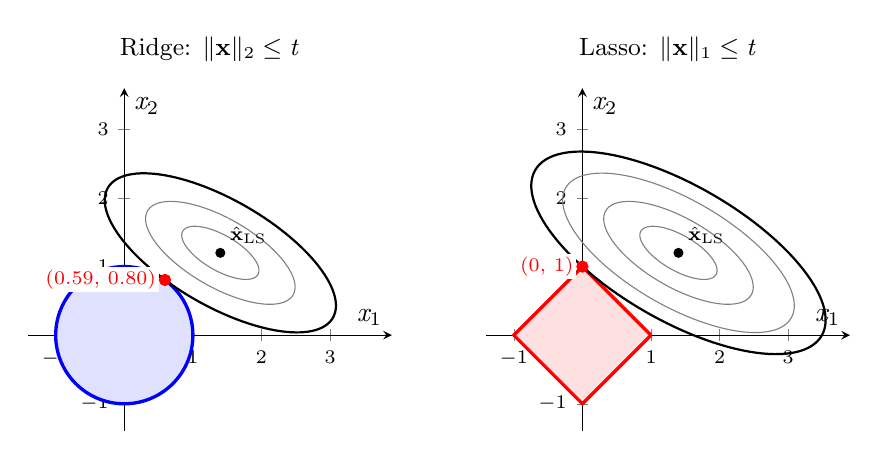
\begin{tikzpicture}
      \begin{groupplot}[group style={group size=2 by 1, horizontal sep=1.2cm}, width=6.2cm, height=6.2cm,
          axis equal image, axis lines=middle, xmin=-1.4, xmax=3.9, ymin=-1.4, ymax=3.6, xtick={-1,1,2,3}, ytick={-1,1,2,3},
          tick label style={font=\scriptsize}, title style={font=\small}, xlabel={$x_1$}, ylabel={$x_2$}]
        \nextgroupplot[title={Ridge: $\|\vect x\|_2\le t$}]
\addplot[blue, very thick, fill=blue!12, domain=0:360, samples=121, variable=\t] ({cos(\t)}, {sin(\t)});
\addplot[gray, thin, domain=0:360, samples=121, variable=\t] ({1.4+0.6325*cos(\t)*0.8660-0.2582*sin(\t)*-0.5000}, {1.2+0.6325*cos(\t)*-0.5000+0.2582*sin(\t)*0.8660});
\addplot[gray, thin, domain=0:360, samples=121, variable=\t] ({1.4+1.2247*cos(\t)*0.8660-0.5000*sin(\t)*-0.5000}, {1.2+1.2247*cos(\t)*-0.5000+0.5000*sin(\t)*0.8660});
\addplot[black, thick, domain=0:360, samples=121, variable=\t] ({1.4+1.8940*cos(\t)*0.8660-0.7730*sin(\t)*-0.5000}, {1.2+1.8940*cos(\t)*-0.5000+0.7730*sin(\t)*0.8660});
\addplot[only marks, mark=*, mark size=1.6pt, black] coordinates {(1.4,1.2)} node[above right, font=\scriptsize] {$\hat{\vect x}_{\text{LS}}$};
\addplot[only marks, mark=*, mark size=2pt, red] coordinates {(0.593,0.805)} node[left, font=\scriptsize, xshift=-2pt, fill=white, inner sep=1pt] {$(0.59,\,0.80)$};
\nextgroupplot[title={Lasso: $\|\vect x\|_1\le t$}]
\addplot[red, very thick, fill=red!12] coordinates {(1,0) (0,1) (-1,0) (0,-1) (1,0)};
\addplot[gray, thin, domain=0:360, samples=121, variable=\t] ({1.4+0.6325*cos(\t)*0.8660-0.2582*sin(\t)*-0.5000}, {1.2+0.6325*cos(\t)*-0.5000+0.2582*sin(\t)*0.8660});
\addplot[gray, thin, domain=0:360, samples=121, variable=\t] ({1.4+1.2247*cos(\t)*0.8660-0.5000*sin(\t)*-0.5000}, {1.2+1.2247*cos(\t)*-0.5000+0.5000*sin(\t)*0.8660});
\addplot[gray, thin, domain=0:360, samples=121, variable=\t] ({1.4+1.8974*cos(\t)*0.8660-0.7746*sin(\t)*-0.5000}, {1.2+1.8974*cos(\t)*-0.5000+0.7746*sin(\t)*0.8660});
\addplot[black, thick, domain=0:360, samples=121, variable=\t] ({1.4+2.4110*cos(\t)*0.8660-0.9840*sin(\t)*-0.5000}, {1.2+2.4110*cos(\t)*-0.5000+0.9840*sin(\t)*0.8660});
\addplot[only marks, mark=*, mark size=1.6pt, black] coordinates {(1.4,1.2)} node[above right, font=\scriptsize] {$\hat{\vect x}_{\text{LS}}$};
\addplot[only marks, mark=*, mark size=2pt, red] coordinates {(0,1)} node[left, font=\scriptsize, xshift=-2pt, fill=white, inner sep=1pt] {$(0,\,1)$};
      \end{groupplot}
    \end{tikzpicture}
    \caption{Why the lasso gives sparse solutions (constrained form with $t=1$; the penalized forms above are equivalent for a suitable $\lambda$). Gray: contour lines of the least-squares cost $\|\mat A\vect x-\vect b\|_2^2$, which are ellipses around the unregularized solution $\hat{\vect x}_{\text{LS}}$. The constrained solution (red dot) is where the smallest contour touches the unit ball (black contour). The round $L_2$ ball is touched at a generic point with both components non-zero. The $L_1$ ball has corners on the axes, and the contour typically touches it at a corner, so $x_1=0$ exactly.}
    \label{fig:ridge_lasso}
  \end{figure}

\subsubsection{Compressed Sensing}\autocite{candes2008,boyd2004}
\begin{itemize}
    \item In the previous chapter we motivated regularized linear regression. 
    \item Assume we have fewer measurements than required to estimate the parameter vector $\vect x$. 
    \item Solution of the underdetermined case required. 
    \item We call a vector $s$-sparse if its support, i.\,e.\ the number of non-zero entries, is less than or equal to $s$ ($S$ is reserved for the training set).  
    \item Under suitable conditions on the sparsity $s$ and on the measurement matrix $\mat A$ (e.\,g.\ a restricted isometry or null-space property), an $s$-sparse vector $\vect x$ is recovered \emph{exactly} from noiseless measurements by solving the convex optimization problem (it can be rewritten as a linear program):
      \begin{eqnarray*}
        \mbox{minimize}   & &\quad \|\vect x\|_1\\
        \mbox{subject to} & & \quad \mat A\vect x =\vect b.
      \end{eqnarray*}
      For noisy measurements the constraint is relaxed, e.\,g.\ to $\|\mat A\vect x-\vect b\|_2\le\varepsilon$, or a penalized form (lasso) is used.
  \end{itemize}

\newpage
\subsection{Convex and Non-Convex Penalty Functions}

  Motivated by the discussion of different norms, we now introduce and study \textbf{penalty functions}. A penalty function $\phi$ assigns a cost to each residual; norms are special cases (e.\,g.\ $\phi(r)=|r|$ or $r^2$), and norms can also be used as regularizers on the parameters (e.\,g.\ $\lambda\|\vect x\|_1$). Both convex and non-convex objectives can be optimized, but convexity is very useful: every local minimum of a convex function is global. Non-convex problems may have several local minima, so finding or certifying the global optimum is harder (see the optimization chapters).\\[0.3cm]
  
  \textbf{Definition}\\
The \emph{penalty function approximation problem} is defined as follows:
    \begin{eqnarray*}
      \mbox{minimize}   & &\sum_{i=1}^m \phi(r_i) \\
      \mbox{subject to} & & \vect r= (r_1, r_2, \dots, r_m)^T = \mat A\vect x -\vect b,
    \end{eqnarray*}
    where $\phi:\real \rightarrow \real$ is the penalty function for the components of the \\
    residual vector.
    
  \textbf{Note:} 
  \begin{itemize}
    \item The penalty function $\phi$ assigns \textbf{costs} to residuals. 
    \item If $\phi$ is a convex function, the penalty function approximation problem is a convex optimization problem.
  \end{itemize}
  Penalty functions of the $L_1$-,  $L_2$-norms:
  \begin{displaymath}
    \phi_{L_1}(r) = |r|;  \qquad \qquad \qquad \qquad \qquad \phi_{L_2}(r) = r^2
  \end{displaymath}
  \begin{itemize}
    \item In $L_1$ small deviations are weighted higher than using $L_2$.
    \item In $L_1$ large deviations are weighted lower than using $L_2$.
  \end{itemize}
 \textbf{Log barrier function} with parameter $a>0$
  \begin{displaymath}
    \phi_\mathsf{barrier}(r) = 
      \left\{
        \begin{array}{cl}
          -a^2\log \left(1-\left( \frac{r}{a}\right)^2 \right),  & \quad \mbox{if} \quad |r| < a\\
          \infty,                                                & \quad \mbox{otherwise}
        \end{array}
      \right.
  \end{displaymath}   
  \textbf{Dead zone linear penalty function} with parameter $a>0$
  \begin{displaymath}
    \phi_\mathsf{dz}(r) = 
      \left\{
        \begin{array}{cl}
          0,     & \quad \mbox{if} \quad |r| \leq a\\
          |r|-a, & \quad \mbox{otherwise}
        \end{array}
      \right.
  \end{displaymath}
  \textbf{Large error penalty function} with parameter $a>0$
  \begin{displaymath}
    \phi_\mathsf{e}(r) = 
      \left\{
        \begin{array}{cl}
          r^2, & \quad \mbox{if} \quad |r| \leq a \\
          a^2, & \quad \mbox{otherwise}
        \end{array}
      \right.
  \end{displaymath}
  \textbf{Huber function} with parameter $a>0$
  \begin{displaymath}
    \phi_\mathsf{Huber}(r) = 
      \left\{
        \begin{array}{cl}
          r^2,            & \quad \mbox{if} \quad |r| \leq a \\
          a\cdot(2|r|-a), & \quad \mbox{otherwise}
        \end{array}
      \right.
  \end{displaymath}
  
\subsection{Lessons Learned}
  \begin{itemize}
    \item We have considered vector and matrix norms in more detail. 
    \item Important vector norms: $L_1$, $L_2$, $L_\infty$, and $L_{\mat P}$. 
    \item Unit balls 
    \item Linear regression for different norms: range from closed form solution to LP-problem.
    \item Regularized linear regression: range from closed form solution through QP-problem up to combinatorial optimization. 
    \item We need to know the basics of algorithms for unconstrained and constrained optimization as well as convex optimization.
  \end{itemize}

\subsection{Comprehensive Questions}
  \begin{itemize}
    \item What is the difference between the $L_p$- (p $\ge$ 1) and the $L_{\mat P}$-norm? 
    \item How do the unit balls look like for $L_{\infty}$-, $L_4$-, $L_2$-, $L_1$- and $L_0$-norm? 
    \item What is the benefit of using the $L_1$- over the $L_2$-norm for sparse, underdetermined problems? 
    \item What specific property of penalty functions is of special interest and why do we need different penalty functions at all? 
  \end{itemize}

\newpage
\section{Rosenblatt's Perceptron (1957)}\autocite{hastie2009,ripley1996,rosenblatt1958}

\subsection{Motivation}

The perceptron, developed by Frank Rosenblatt in 1957, is considered the first model of an artificial neural network. Its goal is to compute a linear decision boundary between two classes. We therefore assume that the classes are \textbf{linearly separable}, i.\,e.\ that there exists a hyperplane which classifies every training example correctly. The learning task is then to compute such a linear separating hyperplane by minimizing the distance of the misclassified feature vectors to the decision boundary.

\subsection{Objective Function}

  Assume the following:
  \begin{itemize}
    \item True class labels are $y_i\in\{-1,+1\}$.
    \item The decision boundary is a linear function with prediction
      \begin{displaymath}
        \hat y = \sign(\vect \alpha^T\vect x + \alpha_0).
      \end{displaymath}
    \item Parameters $\alpha_0$ and $\vect \alpha$ are chosen according to the optimization problem 
      \begin{center}
        $\displaystyle \mbox{minimize} \quad \bigg\{ D(\alpha_0, \vect \alpha)= -\sum_{i\in {\cal M}} y_i \cdot (\vect \alpha^T\vect x_i + \alpha_0) \bigg\}$
      \end{center}
      where $\cal M$ is the set of \textbf{indices} of misclassified samples.
     \item The elements of the sum in the objective function depend on the set $\cal M$.          
    \item In each iteration step the cardinality of $\cal M$ might change.          
    \item The cardinality of $\cal M$ is a discrete variable.
    \item \textbf{Competing variables:} continuous parameters of linear decision boundary and the discrete cardinality of $\cal M$.
  \end{itemize}
 
\subsection{Minimization of Objective Function}

  Remember the objective function $D(\alpha_0, \vect \alpha)$:
  \begin{displaymath}
    \mbox{minimize} \quad \quad D(\alpha_0, \vect \alpha)= -\sum_{i\in {\cal M}} y_i \cdot (\vect \alpha^T\vect x_i + \alpha_0)
  \end{displaymath}
 
  The gradient of the objective function is:          
  \begin{eqnarray*}
    \frac{\partial}{\partial \alpha_0} \ D(\alpha_0, \vect \alpha)&=&  -\sum_{i\in {\cal M}} y_i \\          
    \frac{\partial}{\partial \vect\alpha} \ D(\alpha_0, \vect \alpha)&=& -\sum_{i\in {\cal M}} y_i\cdot  \vect x_i \\
  \end{eqnarray*}
  We want to take an update step right after having visited each misclassified observation.
  The update rule in the $(k+1)$-st iteration step is:

  \begin{displaymath}
    \begin{pmatrix}\alpha_0^{(k+1)}\\ \vect \alpha^{(k+1)}\end{pmatrix} =            \begin{pmatrix}\alpha_0^{(k)}\\ \vect \alpha^{(k)}\end{pmatrix} + \eta \begin{pmatrix}y_i\\ y_i\cdot \vect x_i\end{pmatrix}
  \end{displaymath} 
  Here $\eta>0$ is the learning rate (step size; the same symbol is used in the MLP chapter). With the zero initialization below it can be set to $1$ without loss of generality, since it only scales $(\alpha_0,\vect\alpha)$. The parameters are stacked as $(\alpha_0;\vect\alpha)$ here, while the regression part of Chapter \emph{Discriminant Analysis} stacks $\vect\theta=(\vect\alpha;\alpha_0)$; the order does not matter.
 
  \begin{algorithmic}
    \STATE\textbf{Input:} training data: $S = \{(\vect x_i,y_i)\}_{i=1}^m$ with $y_i\in\{-1,+1\}$.
    \STATE initialize  $k=0$, $\alpha^{(0)}_0=0$ and $\vect \alpha^{(0)}=  \vect 0$
    \Repeat
      \STATE select pair $(\vect x_i, y_i)$ from training set.
      \If{$y_i\cdot (\vect x_i^T \vect\alpha^{(k)} + \alpha_0^{(k)})\leq 0$}
        \STATE
        \STATE $\displaystyle\begin{pmatrix}\alpha_0^{(k+1)}\\ \vect \alpha^{(k+1)}\end{pmatrix} =  \begin{pmatrix}\alpha_0^{(k)}\\ \vect \alpha^{(k)}\end{pmatrix} +  \begin{pmatrix}y_i\\ y_i\cdot \vect x_i\end{pmatrix}$
        \STATE
        \STATE $k\leftarrow k+1$
      \EndIf

    \Until{$y_i\cdot (\vect x_i^T \vect\alpha^{(k)} + \alpha_0^{(k)})> 0 \quad \mbox {for all} \quad i$}
    \STATE \structure{Output:} $\alpha_0^{(k)}$ and $\vect \alpha^{(k)}$
  \end{algorithmic}

Figure~\ref{fig:perceptron_updates} shows the algorithm on a small example.

  \begin{figure}[htbp]
    \centering
    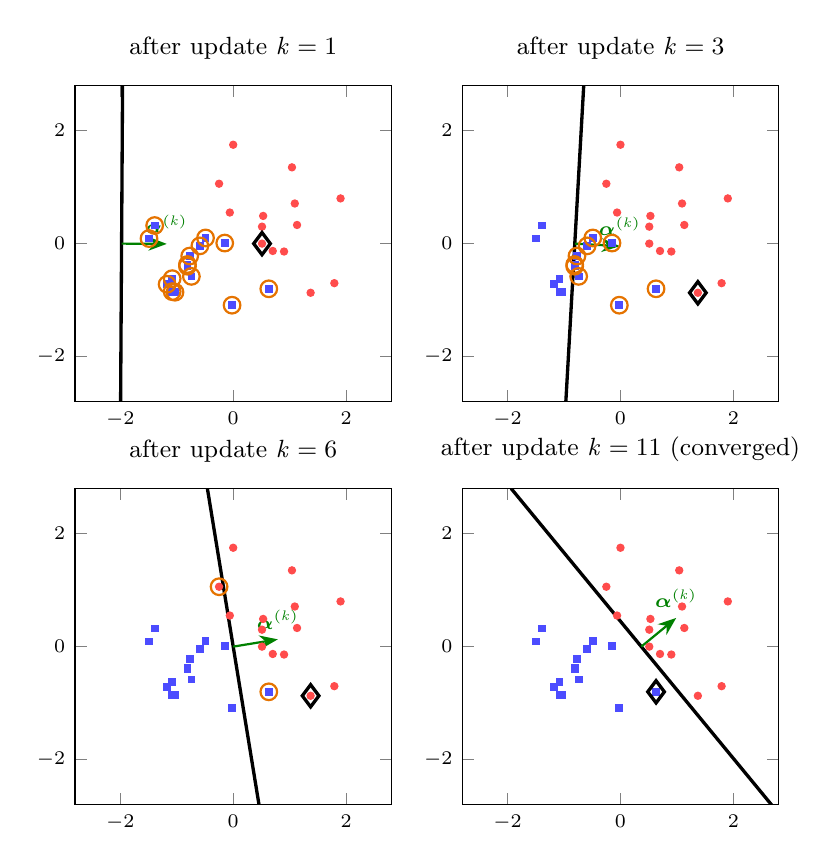
\begin{tikzpicture}
      \begin{groupplot}[group style={group size=2 by 2, horizontal sep=0.9cm, vertical sep=1.1cm}, width=5.6cm, height=5.6cm,
          axis equal image, xmin=-2.8, xmax=2.8, ymin=-2.8, ymax=2.8, xtick={-2,0,2}, ytick={-2,0,2},
          tick label style={font=\scriptsize}, title style={font=\small}]
        \nextgroupplot[title={after update $k=1$}]
\addplot[only marks, mark=*, mark size=1.3pt, red!70] coordinates {(0.51,0.30) (1.90,0.80) (0.53,0.49) (-0.06,0.55) (1.04,1.35) (1.09,0.71) (0.00,1.75) (-0.25,1.06) (0.70,-0.13) (0.51,-0.00) (1.13,0.33) (1.79,-0.70) (0.90,-0.14) (1.37,-0.87)};
\addplot[only marks, mark=square*, mark size=1.2pt, blue!70] coordinates {(-0.81,-0.37) (-1.49,0.09) (-0.49,0.10) (-0.02,-1.09) (-1.08,-0.62) (-0.15,0.01) (-1.03,-0.86) (-1.08,-0.85) (-0.74,-0.58) (0.63,-0.80) (-0.77,-0.22) (-1.17,-0.72) (-0.59,-0.04) (-1.39,0.32) (-0.81,-0.40)};
\addplot[only marks, mark=o, mark size=3pt, thick, orange!90!black] coordinates {(-0.81,-0.37) (-1.49,0.09) (-0.49,0.10) (-0.02,-1.09) (-1.08,-0.62) (-0.15,0.01) (-1.03,-0.86) (-1.08,-0.85) (-0.74,-0.58) (0.63,-0.80) (-0.77,-0.22) (-1.17,-0.72) (-0.59,-0.04) (-1.39,0.32) (-0.81,-0.40)};
\addplot[only marks, mark=diamond, mark size=4pt, very thick, black] coordinates {(0.51,-0.00)};
\addplot[black, very thick] coordinates {(-1.993,-2.800) (-1.958,2.800)};
\draw[-{Stealth}, thick, green!50!black] (axis cs:-1.976,0.000) -- (axis cs:-1.176,-0.005) node[above, font=\scriptsize] {$\vect\alpha^{(k)}$};
        \nextgroupplot[title={after update $k=3$}]
\addplot[only marks, mark=*, mark size=1.3pt, red!70] coordinates {(0.51,0.30) (1.90,0.80) (0.53,0.49) (-0.06,0.55) (1.04,1.35) (1.09,0.71) (0.00,1.75) (-0.25,1.06) (0.70,-0.13) (0.51,-0.00) (1.13,0.33) (1.79,-0.70) (0.90,-0.14) (1.37,-0.87)};
\addplot[only marks, mark=square*, mark size=1.2pt, blue!70] coordinates {(-0.81,-0.37) (-1.49,0.09) (-0.49,0.10) (-0.02,-1.09) (-1.08,-0.62) (-0.15,0.01) (-1.03,-0.86) (-1.08,-0.85) (-0.74,-0.58) (0.63,-0.80) (-0.77,-0.22) (-1.17,-0.72) (-0.59,-0.04) (-1.39,0.32) (-0.81,-0.40)};
\addplot[only marks, mark=o, mark size=3pt, thick, orange!90!black] coordinates {(-0.81,-0.37) (-0.49,0.10) (-0.02,-1.09) (-0.15,0.01) (-0.74,-0.58) (0.63,-0.80) (-0.77,-0.22) (-0.59,-0.04) (-0.81,-0.40)};
\addplot[only marks, mark=diamond, mark size=4pt, very thick, black] coordinates {(1.37,-0.87)};
\addplot[black, very thick] coordinates {(-0.967,-2.800) (-0.650,2.800)};
\draw[-{Stealth}, thick, green!50!black] (axis cs:-0.808,0.000) -- (axis cs:-0.010,-0.045) node[above, font=\scriptsize] {$\vect\alpha^{(k)}$};
        \nextgroupplot[title={after update $k=6$}]
\addplot[only marks, mark=*, mark size=1.3pt, red!70] coordinates {(0.51,0.30) (1.90,0.80) (0.53,0.49) (-0.06,0.55) (1.04,1.35) (1.09,0.71) (0.00,1.75) (-0.25,1.06) (0.70,-0.13) (0.51,-0.00) (1.13,0.33) (1.79,-0.70) (0.90,-0.14) (1.37,-0.87)};
\addplot[only marks, mark=square*, mark size=1.2pt, blue!70] coordinates {(-0.81,-0.37) (-1.49,0.09) (-0.49,0.10) (-0.02,-1.09) (-1.08,-0.62) (-0.15,0.01) (-1.03,-0.86) (-1.08,-0.85) (-0.74,-0.58) (0.63,-0.80) (-0.77,-0.22) (-1.17,-0.72) (-0.59,-0.04) (-1.39,0.32) (-0.81,-0.40)};
\addplot[only marks, mark=o, mark size=3pt, thick, orange!90!black] coordinates {(-0.25,1.06) (0.63,-0.80)};
\addplot[only marks, mark=diamond, mark size=4pt, very thick, black] coordinates {(1.37,-0.87)};
\addplot[black, very thick] coordinates {(-0.457,2.800) (0.457,-2.800)};
\draw[-{Stealth}, thick, green!50!black] (axis cs:0.000,0.000) -- (axis cs:0.790,0.129) node[above, font=\scriptsize] {$\vect\alpha^{(k)}$};
        \nextgroupplot[title={after update $k=11$ (converged)}]
\addplot[only marks, mark=*, mark size=1.3pt, red!70] coordinates {(0.51,0.30) (1.90,0.80) (0.53,0.49) (-0.06,0.55) (1.04,1.35) (1.09,0.71) (0.00,1.75) (-0.25,1.06) (0.70,-0.13) (0.51,-0.00) (1.13,0.33) (1.79,-0.70) (0.90,-0.14) (1.37,-0.87)};
\addplot[only marks, mark=square*, mark size=1.2pt, blue!70] coordinates {(-0.81,-0.37) (-1.49,0.09) (-0.49,0.10) (-0.02,-1.09) (-1.08,-0.62) (-0.15,0.01) (-1.03,-0.86) (-1.08,-0.85) (-0.74,-0.58) (0.63,-0.80) (-0.77,-0.22) (-1.17,-0.72) (-0.59,-0.04) (-1.39,0.32) (-0.81,-0.40)};
\addplot[only marks, mark=diamond, mark size=4pt, very thick, black] coordinates {(0.63,-0.80)};
\addplot[black, very thick] coordinates {(-1.936,2.800) (2.674,-2.800)};
\draw[-{Stealth}, thick, green!50!black] (axis cs:0.369,0.000) -- (axis cs:0.987,0.508) node[above, font=\scriptsize] {$\vect\alpha^{(k)}$};
      \end{groupplot}
    \end{tikzpicture}
    \caption{Perceptron learning on a linearly separable toy set (red circles: $y=+1$, blue squares: $y=-1$), zero initialization, learning rate $1$. Each update adds $y_i(1,\vect x_i^T)^T$ of the currently visited misclassified sample (black diamond) to $(\alpha_0,\vect\alpha^T)^T$, which rotates and shifts the boundary $\vect\alpha^T\vect x+\alpha_0=0$ (black; the green arrow is the normal $\vect\alpha^{(k)}$ pointing to the $\hat y=+1$ side). Orange rings mark the samples that are still misclassified. Here the algorithm stops after $11$ updates, well below the Novikoff bound (Fig.~\ref{fig:perceptron_margin}).}
    \label{fig:perceptron_updates}
  \end{figure}

\subsection{Remarks on Perceptron Learning}

  \begin{itemize}
    \item The update rule is extremely simple. \\[.3cm]
    \item Nothing happens if we classify all $\vect x_i$ correctly using the given linear decision boundary. 
    \item The parameter $\vect \alpha$ of the decision boundary is a linear combination of feature vectors. 
    \item The decision boundary thus is:
    \begin{displaymath}
       f(\vect x) = \left (\sum_{i\in \cal E} y_i\cdot \vect x_i \right)^T \vect x + \sum_{i\in \cal E} y_i \quad 
                 = \quad \sum_{i\in \cal E} y_i\cdot \langle \vect x_i, \vect x\rangle + \sum_{i\in \cal E} y_i 
    \end{displaymath}
    with $\hat y=\sign(f(\vect x))$, where $\cal E$ is the list of indices that required an update (indices may appear more than once); this assumes zero initialization and $\eta=1$. 
    \item The final linear decision boundary depends on the initialization, \\
      i.\,e.\ $\alpha_0^{(0)}$ and $\vect \alpha^{(0)}$. 
    \item The number of iterations can be rather large. 
    \item If data are not linearly separable, the proposed learning algorithm will not converge. The algorithm will end up in hard to detect cycles.
  \end{itemize}

\subsection{Convergence of Learning Algorithm}

The derivation is not important for the exam. It is important to understand that, for linearly separable data, there is an \emph{upper bound} on the number of updates the perceptron makes before it classifies all training samples correctly. The bound depends on the margin $\rho$, the data radius $R$ and the offset $\alpha_0^*$ of the separating hyperplane, not explicitly on the feature dimension. 

 \textbf{Convergence Theorem of Rosenblatt and Novikoff}\\
    Assume that for all $i=1,2, \dots, m$
    \begin{displaymath}
      y_i(\vect x_i^T\vect \alpha^* +\alpha^*_0)\geq \rho
    \end{displaymath}
    for some $(\alpha_0^*,\vect\alpha^*)$ with $\rho>0$ and $\|\vect \alpha^*\|_2=1$ (i.\,e.\ the data are linearly separable with margin $\rho$).
    Let $R= \max_i \|\vect x_i\|_2$. \\
    
Then the perceptron learning algorithm with zero initialization makes at most $k$ updates (and then separates the training data), where
    \begin{displaymath}
      k \leq \frac{(\alpha_0^{*2}+1)(1+R^2)}{\rho^2}.
    \end{displaymath}
    The quantities $\rho$ and $R$ are illustrated in Fig.~\ref{fig:perceptron_margin}.

  \begin{figure}[htbp]
    \centering
    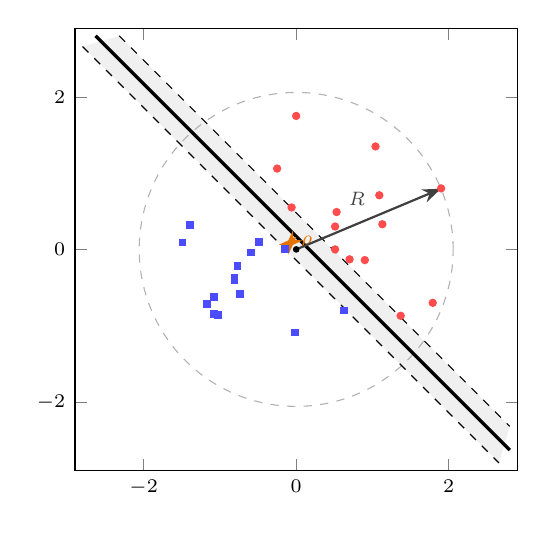
\begin{tikzpicture}
      \begin{axis}[width=7.2cm, height=7.2cm, axis equal image, xmin=-2.9, xmax=2.9, ymin=-2.9, ymax=2.9,
          xtick={-2,0,2}, ytick={-2,0,2}, tick label style={font=\scriptsize}, clip=false]
        \fill[gray!12] (axis cs:-2.320,2.800) -- (axis cs:2.800,-2.320) -- (axis cs:2.659,-2.800) -- (axis cs:-2.800,2.659) -- cycle;
        \draw[gray!60, dashed] (axis cs:0,0) circle [radius=2.058];
        \addplot[only marks, mark=*, mark size=1.3pt, red!70] coordinates {(0.51,0.30) (1.90,0.80) (0.53,0.49) (-0.06,0.55) (1.04,1.35) (1.09,0.71) (0.00,1.75) (-0.25,1.06) (0.70,-0.13) (0.51,-0.00) (1.13,0.33) (1.79,-0.70) (0.90,-0.14) (1.37,-0.87)};
        \addplot[only marks, mark=square*, mark size=1.2pt, blue!70] coordinates {(-0.81,-0.37) (-1.49,0.09) (-0.49,0.10) (-0.02,-1.09) (-1.08,-0.62) (-0.15,0.01) (-1.03,-0.86) (-1.08,-0.85) (-0.74,-0.58) (0.63,-0.80) (-0.77,-0.22) (-1.17,-0.72) (-0.59,-0.04) (-1.39,0.32) (-0.81,-0.40)};
        \addplot[black, very thick] coordinates {(-2.630,2.800) (2.800,-2.630)};
        \addplot[black, dashed] coordinates {(-2.320,2.800) (2.800,-2.320)};
        \addplot[black, dashed] coordinates {(-2.800,2.659) (2.659,-2.800)};
        \draw[{Stealth}-{Stealth}, thick, orange!90!black] (axis cs:-0.151,0.011) -- (axis cs:0.004,0.166) node[midway, right, font=\scriptsize] {$\rho$};
        \draw[-{Stealth}, thick, gray!50!black] (axis cs:0,0) -- (axis cs:1.898,0.795) node[pos=0.55, above left, font=\scriptsize] {$R$};
        \fill (axis cs:0,0) circle (1.2pt);
      \end{axis}
    \end{tikzpicture}
    \caption{Quantities in the convergence theorem of Rosenblatt and Novikoff for the data of Fig.~\ref{fig:perceptron_updates}. A unit-norm separator $(\alpha_0^*,\vect\alpha^*)$ (black) classifies every sample with $y_i(\vect x_i^T\vect\alpha^*+\alpha_0^*)\ge\rho$, i.\,e.\ every sample lies at least the distance $\rho$ from the boundary (gray band). $R=\max_i\|\vect x_i\|_2$ is the radius of the smallest origin-centered circle containing all samples (dashed). The number of updates is at most $(\alpha_0^{*2}+1)(1+R^2)/\rho^2$: small margins or large radii allow more updates. Here, for the largest-margin separator, $\rho\approx0.22$, $R\approx2.06$, and the bound is about $110$ updates.}
    \label{fig:perceptron_margin}
  \end{figure}
  Let us look at the estimated parameters after $k$ updates and how the parameters change with each update. The $k$-th update is made with a sample $(\vect x_i,y_i)$ that is misclassified by $(\alpha_0^{(k-1)},\vect\alpha^{(k-1)})$. Using the assumption and induction from $(\alpha_0^{(0)},\vect\alpha^{(0)})=\vect 0$:

  \begin{eqnarray*}
    \begin{pmatrix}\alpha_0^{(k)}\\ \vect \alpha^{(k)}\end{pmatrix}^T\begin{pmatrix}\alpha_0^*\\ \vect \alpha^*\end{pmatrix} 
      &=&           \left( \begin{pmatrix}\alpha_0^{(k-1)}\\ \vect \alpha^{(k-1)}\end{pmatrix} +  \begin{pmatrix}y_i\\ y_i\cdot \vect x_i\end{pmatrix}\right)^T \begin{pmatrix}\alpha_0^*\\ \vect \alpha^*\end{pmatrix}\\          
      &=& \begin{pmatrix}\alpha_0^{(k-1)}\\ \vect \alpha^{(k-1)}\end{pmatrix} ^T\begin{pmatrix}\alpha_0^*\\ \vect \alpha^*\end{pmatrix} +  \begin{pmatrix}y_i\\ y_i\cdot \vect x_i\end{pmatrix}^T \begin{pmatrix}\alpha_0^*\\ \vect \alpha^*\end{pmatrix} \\          
      &\geq& \begin{pmatrix}\alpha_0^{(k-1)}\\ \vect \alpha^{(k-1)}\end{pmatrix} ^T\begin{pmatrix}\alpha_0^*\\ \vect \alpha^*\end{pmatrix} + \rho \\         &\geq& k\rho
  \end{eqnarray*}
\textbf{Conclusion:} The more iterations (i.\,e.\ misclassifications) we have, the more the vectors are aligned. Now we apply the Cauchy-Schwarz inequality for inner products:

  \begin{eqnarray*}
    \begin{pmatrix}\alpha_0^{(k)}\\ \vect \alpha^{(k)}\end{pmatrix}^T\begin{pmatrix}\alpha_0^*\\ \vect \alpha^*\end{pmatrix} 
      &\leq& \left\|  \begin{pmatrix}\alpha_0^{(k)}\\ \vect \alpha^{(k)}\end{pmatrix}\right\|_2\cdot  \left\| \begin{pmatrix}\alpha_0^*\\ \vect \alpha^*\end{pmatrix}\right\|_2 \\[.5cm]          
      &=&\left \|  \begin{pmatrix}\alpha_0^{(k)}\\ \vect \alpha^{(k)}\end{pmatrix}\right\|_2\cdot  \sqrt{\alpha_0^{*2}+1}
  \end{eqnarray*}
  The norm of the vector estimated in the $k$-th iteration step is:
  \begin{eqnarray*}
    & &  \left \|  \begin{pmatrix}\alpha_0^{(k)}\\ \vect \alpha^{(k)}\end{pmatrix}\right\|_2^2 =
   \left\| \begin{pmatrix}\alpha_0^{(k-1)}\\ \vect \alpha^{(k-1)}\end{pmatrix} +  \begin{pmatrix}y_i\\ y_i\cdot \vect x_i\end{pmatrix}\right\|_2^2 \\         
   & & \vspace*{-2cm} = \begin{pmatrix}\alpha_0^{(k-1)}\\ \vect \alpha^{(k-1)}\end{pmatrix} ^T\begin{pmatrix}\alpha_0^{(k-1)}\\ \vect \alpha^{(k-1)}\end{pmatrix} 
           + 2 \begin{pmatrix}\alpha_0^{(k-1)}\\ \vect \alpha^{(k-1)}\end{pmatrix}^T\begin{pmatrix}y_i\\ y_i\cdot \vect x_i\end{pmatrix}
          + \begin{pmatrix}y_i\\ y_i\cdot \vect x_i\end{pmatrix}^T\begin{pmatrix}y_i\\ y_i\cdot \vect x_i\end{pmatrix}
  \end{eqnarray*}
  The $k$-th update is only made if $\vect x_i$ is misclassified by the previous parameters:
  
  \begin{displaymath}
    \begin{pmatrix}\alpha_0^{(k-1)}\\ \vect \alpha^{(k-1)}\end{pmatrix}^T\begin{pmatrix}y_i\\ y_i\cdot \vect x_i\end{pmatrix}
    = y_i\cdot (\vect x_i^T \vect\alpha^{(k-1)} + \alpha_0^{(k-1)})\quad \leq \quad 0
  \end{displaymath}
  (The non-strict inequality is needed: with the zero initialization the first update happens at equality.)
  Since $\|(y_i,\,y_i\vect x_i^T)^T\|_2^2=1+\|\vect x_i\|_2^2\le 1+R^2$, induction gives
  \begin{displaymath}
    \left \|  \begin{pmatrix}\alpha_0^{(k)}\\ \vect \alpha^{(k)}\end{pmatrix}\right\|_2^2 
    \leq \begin{pmatrix}\alpha_0^{(k-1)}\\ \vect \alpha^{(k-1)}\end{pmatrix} ^T\begin{pmatrix}\alpha_0^{(k-1)}\\ \vect \alpha^{(k-1)}\end{pmatrix} 
           + \begin{pmatrix}y_i\\ y_i\cdot \vect x_i\end{pmatrix}^T\begin{pmatrix}y_i\\ y_i\cdot \vect x_i\end{pmatrix}
    \leq k(1+R^2)
  \end{displaymath}
  Wrap-up:
  \begin{displaymath}
    k\rho 
    \leq \begin{pmatrix}\alpha_0^{(k)}\\ \vect \alpha^{(k)}\end{pmatrix}^T\begin{pmatrix}\alpha_0^*\\ \vect \alpha^*\end{pmatrix} 
    \leq \left \|  \begin{pmatrix}\alpha_0^{(k)}\\ \vect \alpha^{(k)}\end{pmatrix}\right\|_2\cdot  \sqrt{\alpha_0^{*2}+1}
  \end{displaymath}
  Using the Cauchy-Schwarz inequality:
  \begin{displaymath}
    k\rho\quad
    \leq \quad \left \| \begin{pmatrix}\alpha_0^{(k)}\\ \vect \alpha^{(k)}\end{pmatrix}\right\|_2\cdot  \sqrt{\alpha_0^{*2}+1}\quad \leq \quad  \sqrt{k(1+R^2)(\alpha_0^{*2}+1)}
  \end{displaymath}
  shows:
  \begin{displaymath}
    k \quad \leq\quad \frac{(\alpha_0^{*2}+1)(1+R^2)}{\rho^2}
  \end{displaymath}
  
\subsection{Lessons Learned}

  \begin{itemize}
    \item Objective function changes in each iteration step. 
    \item Optimization problem is discrete.
    \item Very simple learning rule.
    \item \vorsicht \structure{Very important:} The bound on the number of updates does \structure{not} depend on the dimension of the feature vectors.
  \end{itemize}
 
\subsection{Comprehensive Questions}

  \begin{itemize}
    \item What is Rosenblatt's perceptron? 
    \item What is the objective function for Rosenblatt's perceptron? 
    \item Why is the optimization of the objective function nonlinear? 
    \item When and how does Rosenblatt's perceptron algorithm converge?
  \end{itemize}
 
 \newpage
\section{Multi-Layer Perceptrons}

The basics of neural networks, activation functions, and backpropagation (covered in greater detail in the Deep Learning course).\autocite{bishop2006,hastie2009}

\subsection{Physiological Motivation}

The biological neuron provides the conceptual foundation for artificial neural networks. A neuron receives incoming signals through its dendrites; the cell body (soma) integrates them, and at the axon hillock it is decided whether an action potential is fired. The axon then propagates the signal away from the soma to the synaptic terminals, where neurotransmitters are released onto the receptors of neighboring neurons. Biophysical models such as the Hodgkin--Huxley equations describe how action potentials are generated and propagated.

Abstracting the neuron to a computational unit that sums weighted inputs, subtracts a threshold, and passes the result through a non-linear activation function gives the \textbf{artificial neuron} on which the Multi-Layer Perceptron (MLP) is built. Rosenblatt's perceptron used a hard step activation with a binary ``all-or-none'' output, mirroring the observation that a biological neuron fires only when its membrane potential exceeds a threshold. Modern MLPs replace this discontinuous step by smooth (e.\,g.\ sigmoid) or piecewise-linear (e.\,g.\ ReLU) functions, which makes gradient-based learning by backpropagation possible.

\subsection{Topology and Activation Functions}

\textbf{Notation}
{\small
\begin{itemize}
  \item Layers $l=0,1,\dots,L$: layer $0$ is the input layer, layer $L$ the output layer ($L$: number of non-input layers).
  \item $M^{(l)}$: number of neurons in layer $l$.
  \item $y_j^{(l)}$: output of neuron $j$ in layer $l$; the input layer passes the feature vector through: $y_i^{(0)} = x_i$, i.\,e.\ $\vect y^{(0)}=\vect x$.
  \item $w_{ij}^{(l)}$: weight of the connection from neuron $i$ in layer $l-1$ to neuron $j$ in layer $l$; $w_{0j}^{(l)}$: threshold (bias) of neuron $j$; $\vect w$: vector of all weights.
  \item $\text{net}_j^{(l)}$: net input of neuron $j$ in layer $l$; $f$: activation function.
  \item \textbf{Network output (prediction):} $\hat y_k = y_k^{(L)}$, $k=1,\dots,M^{(L)}$.
  \item \textbf{Target (true value)} of a training pattern $(\vect x, \vect y)$: $y_k$ (no layer superscript), $k=1,\dots,M^{(L)}$.
\end{itemize}
}

\textbf{Activation Functions}
\begin{displaymath}
  \text{net}_j^{(l)} = \sum_{i=1}^{M^{(l-1)}} y_i^{(l-1)} w_{ij}^{(l)} - w_{0j}^{(l)},
  \qquad
  y_j^{(l)} = f(\text{net}_j^{(l)})
\end{displaymath}
{\small The threshold $w_{0j}^{(l)}$ enters with a negative sign: neuron $j$ ``fires'' if the weighted input exceeds $w_{0j}^{(l)}$ (equivalently: a constant input $y_0^{(l-1)}=-1$ with weight $w_{0j}^{(l)}$).}
Figure~\ref{fig:mlp_topology} illustrates the notation, and Fig.~\ref{fig:mlp_activations} shows common activation functions $f$.

  \begin{figure}[htbp]
    \centering
    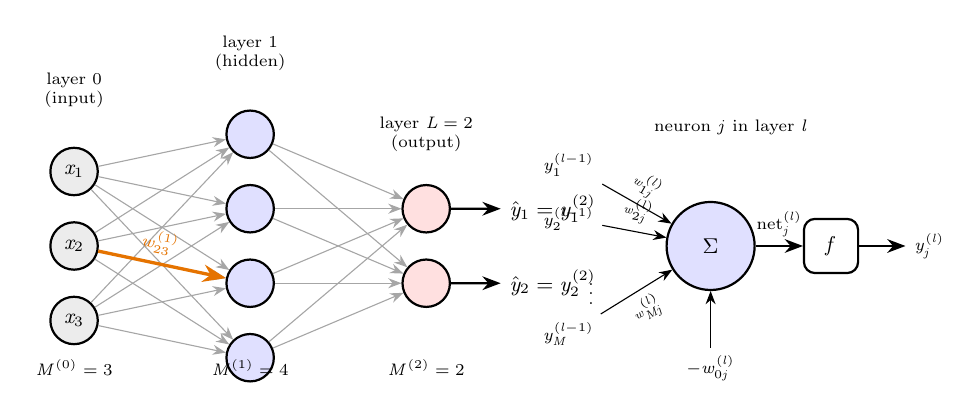
\begin{tikzpicture}[scale=0.86, transform shape, >={Stealth}, font=\small,
        neu/.style={circle, draw, thick, minimum size=7mm, inner sep=0pt},
        inp/.style={neu, fill=gray!15}, hid/.style={neu, fill=blue!12}, outn/.style={neu, fill=red!12}]
      % layer 0
      \foreach \i in {1,2,3} {\node[inp] (x\i) at (0,-1.1*\i) {$x_{\i}$};}
      % layer 1
      \foreach \j in {1,2,3,4} {\node[hid] (h\j) at (2.6,-1.1*\j+0.55) {};}
      % layer 2
      \foreach \k in {1,2} {\node[outn] (o\k) at (5.2,-1.1*\k-0.55) {};}
      \foreach \i in {1,2,3} \foreach \j in {1,2,3,4} {\draw[->, gray!70] (x\i) -- (h\j);}
      \foreach \j in {1,2,3,4} \foreach \k in {1,2} {\draw[->, gray!70] (h\j) -- (o\k);}
      \draw[->, very thick, orange!90!black] (x2) -- node[above, sloped, font=\scriptsize, pos=0.45] {$w_{23}^{(1)}$} (h3);
      \foreach \k in {1,2} {\draw[->, thick] (o\k) -- ++(1.1,0) node[right] {$\hat y_{\k}=y_{\k}^{(2)}$};}
      \node[font=\scriptsize, align=center] at (0,0.1) {layer $0$\\(input)};
      \node[font=\scriptsize, align=center] at (2.6,0.65) {layer $1$\\(hidden)};
      \node[font=\scriptsize, align=center] at (5.2,-0.55) {layer $L=2$\\(output)};
      \node[font=\scriptsize] at (0,-4.0) {$M^{(0)}=3$};
      \node[font=\scriptsize] at (2.6,-4.0) {$M^{(1)}=4$};
      \node[font=\scriptsize] at (5.2,-4.0) {$M^{(2)}=2$};
      % zoom: single neuron
      \begin{scope}[xshift=9.4cm, yshift=-2.2cm]
        \node[hid, minimum size=13mm] (s) at (0,0) {$\Sigma$};
        \node[draw, thick, rounded corners, minimum size=8mm, right=0.7cm of s] (f) {$f$};
        \foreach \i/\yy/\lab in {1/1.2/{y_1^{(l-1)}}, 2/0.4/{y_2^{(l-1)}}, 3/-0.6/{\vdots}, 4/-1.3/{y_{M}^{(l-1)}}} {
          \node[anchor=east, font=\scriptsize] (in\i) at (-1.6,\yy) {$\lab$};}
        \draw[->] (in1) -- node[above, font=\tiny, sloped] {$w_{1j}^{(l)}$} (s);
        \draw[->] (in2) -- node[above, font=\tiny, sloped] {$w_{2j}^{(l)}$} (s);
        \draw[->] (in4) -- node[below, font=\tiny, sloped] {$w_{Mj}^{(l)}$} (s);
        \draw[->] (0,-1.5) node[below, font=\scriptsize] {$-w_{0j}^{(l)}$} -- (s);
        \draw[->, thick] (s) -- node[above, font=\scriptsize] {$\text{net}_j^{(l)}$} (f);
        \draw[->, thick] (f) -- ++(1.1,0) node[right, font=\scriptsize] {$y_j^{(l)}$};
        \node[font=\scriptsize] at (0.3,1.75) {neuron $j$ in layer $l$};
      \end{scope}
    \end{tikzpicture}
    \caption{Left: topology of an MLP with one hidden layer ($L=2$ non-input layers, $M^{(0)}=3$ inputs, $M^{(1)}=4$ hidden neurons, $M^{(2)}=2$ outputs). Each neuron is connected to all neurons of the previous layer; the highlighted connection carries the weight $w_{23}^{(1)}$ from neuron $2$ of layer $0$ to neuron $3$ of layer $1$. Right: a single neuron computes the net input $\text{net}_j^{(l)}=\sum_i y_i^{(l-1)}w_{ij}^{(l)}-w_{0j}^{(l)}$ and outputs $y_j^{(l)}=f(\text{net}_j^{(l)})$ (here $M=M^{(l-1)}$).}
    \label{fig:mlp_topology}
  \end{figure}

  \begin{figure}[htbp]
    \centering
    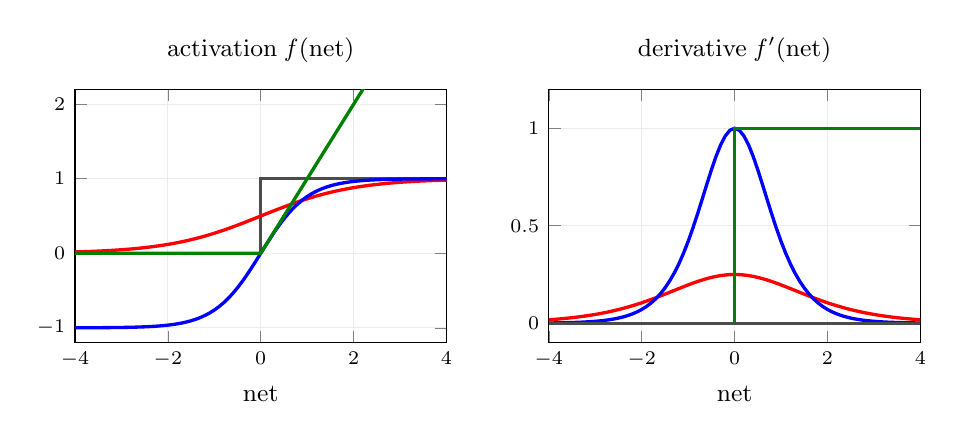
\begin{tikzpicture}
      \begin{groupplot}[group style={group size=2 by 1, horizontal sep=1.3cm}, width=6.3cm, height=4.8cm,
          xmin=-4, xmax=4, xlabel={$\text{net}$}, tick label style={font=\scriptsize}, label style={font=\small}, title style={font=\small},
          grid=major, grid style={gray!15}]
        \nextgroupplot[title={activation $f(\text{net})$}, ymin=-1.2, ymax=2.2, legend to name=actleg, legend columns=4,
            legend style={font=\scriptsize, draw=none}]
          \addplot[gray!60!black, very thick, const plot] coordinates {(-4,0) (0,1) (4,1)};
          \addlegendentry{step (Heaviside)}
          \addplot[red, very thick, domain=-4:4, samples=81] {1/(1+exp(-x))};
          \addlegendentry{sigmoid $\frac{1}{1+e^{-\text{net}}}$}
          \addplot[blue, very thick, domain=-4:4, samples=81] {tanh(x)};
          \addlegendentry{$\tanh(\text{net})$}
          \addplot[green!50!black, very thick, domain=-4:4, samples=81] {max(0,x)};
          \addlegendentry{ReLU $\max(0,\text{net})$}
        \nextgroupplot[title={derivative $f'(\text{net})$}, ymin=-0.1, ymax=1.2]
          \addplot[red, very thick, domain=-4:4, samples=81] {exp(-x)/(1+exp(-x))^2};
          \addplot[blue, very thick, domain=-4:4, samples=81] {1-tanh(x)^2};
          \addplot[green!50!black, very thick, const plot] coordinates {(-4,0) (0,1) (4,1)};
          \draw[gray!60!black, very thick] (axis cs:-4,0) -- (axis cs:4,0);
      \end{groupplot}
    \end{tikzpicture}

    \ref*{actleg}
    \caption{Common activation functions (left) and their derivatives (right). The step function of Rosenblatt's perceptron has derivative $0$ almost everywhere, so it cannot be trained by gradient descent. The sigmoid and $\tanh$ are smooth, but their derivatives vanish for large $|\text{net}|$ (the sigmoid derivative is at most $\frac14$), which slows down backpropagation through many layers (vanishing gradients). ReLU has derivative $1$ for all positive inputs.}
    \label{fig:mlp_activations}
  \end{figure}

\subsection{Backpropagation Algorithm}

  \subsubsection{Supervised Learning Algorithm}

  \begin{itemize}
    \item Gradient descent to adjust the weights reducing the training error $\varepsilon$:
      \begin{displaymath}
        \Delta w_{ij}^{(l)} = - \eta \, \frac{\partial \varepsilon}{\partial w_{ij}^{(l)}}
      \end{displaymath}
      where $\eta>0$ is the \textbf{learning rate}.

    \item Typical error function: \textbf{squared error} of one training pattern $(\vect x, \vect y)$
      \begin{displaymath}
        \varepsilon(\vect w) = \frac{1}{2} \sum_{k=1}^{M^{(L)}} (y_k - \hat y_k)^2, \qquad \hat y_k = y_k^{(L)}
      \end{displaymath}
      where $\vect w$ denotes the vector of all weights. Summing (averaging) over all training patterns gives the (mean) squared error of the training set.
  \end{itemize}

\renewcommand{\err}{\varepsilon}
\newcommand{\net}[2]{\text{net}_{#1}^{(#2)}}
\newcommand{\w}[2]{w_{#1}^{(#2)}}
\newcommand{\y}[2]{y_{#1}^{(#2)}}

Adjusting the weights $\w{jk}{L}$ of the output layer
      \footnotesize
      \begin{displaymath}
        \frac{\partial \err}{\partial \w{jk}{L}} =
        \frac{\partial \err}{\partial \net{k}{L}} \cdot \frac{\partial \net{k}{L}}{\partial \w{jk}{L}} =
        - \delta_k^{(L)} \cdot y_j^{(L-1)}
      \end{displaymath}
   The \emph{sensitivity} $\delta_k^{(L)}$ (with $\hat y_k = \y{k}{L}$):

      \footnotesize
      \begin{eqnarray*}
        \delta_k^{(L)}
        & = & - \frac{\partial \err}{\partial \net{k}{L}}
          =   - \frac{\partial \err}{\partial \hat y_k} \cdot \frac{\partial \hat y_k}{\partial \net{k}{L}} \\
        & = & (y_k - \hat y_k) \, f'(\net{k}{L})
      \end{eqnarray*}

Adjusting the weights $\w{ij}{l}$ of the hidden layers
  \begin{itemize}
    \item Desired output values for the hidden layers are not known.
    \item For the weights $\w{ij}{L-1}$ of the last hidden layer:
  \end{itemize}
      \footnotesize
      \begin{eqnarray*}
        \frac{\partial \err}{\partial \w{ij}{L-1}} & = &
        \frac{\partial \err}{\partial \y{j}{L-1}} \cdot
        \frac{\partial \y{j}{L-1}}{\partial \net{j}{L-1}} \cdot
        \frac{\partial \net{j}{L-1}}{\partial \w{ij}{L-1}} \\
        & = & \frac{\partial \err}{\partial \y{j}{L-1}} \cdot
        f'(\net{j}{L-1}) \cdot \y{i}{L-2}
      \end{eqnarray*}

   \begin{itemize}
     \item {\small The differentiation of $\partial \err$ w.\,r.\,t.\ $\y{j}{L-1}$ can be computed as the sum of the sensitivity values $\delta_k^{(L)}$ of the layer above weighted by the weights $\w{jk}{L}$:}
   \end{itemize}
   \footnotesize
      \begin{eqnarray*}
        \frac{\partial \err}{\partial \y{j}{L-1}} & = &
        \frac{\partial}{\partial \y{j}{L-1}} \Bigg[
          \frac{1}{2} \sum_{k=1}^{M^{(L)}} (y_k - \hat y_k)^2  \Bigg] \\ 
        & = & - \sum_{k=1}^{M^{(L)}} (y_k - \hat y_k) \, \frac{\partial\hat y_k}{\partial\y{j}{L-1}} \\
        & = & - \sum_{k=1}^{M^{(L)}} (y_k - \hat y_k) \, \frac{\partial\hat y_k}{\partial\net{k}{L}} \cdot    \frac{\partial\net{k}{L}}{\partial\y{j}{L-1}} \nonumber \\
        & = & - \sum_{k=1}^{M^{(L)}} (y_k - \hat y_k) \, f'(\net{k}{L}) \, \w{jk}{L} \\
        & = & - \sum_{k=1}^{M^{(L)}} \delta_k^{(L)} \w{jk}{L}
      \end{eqnarray*}

  Sensitivity $\delta_j^{(l)}$ for any hidden layer $l$, $0<l<L$:
  \begin{displaymath}
    \delta_j^{(l)} = f'(\net{j}{l}) \, \sum_{k=1}^{M^{(l+1)}} \w{jk}{l+1} \, \delta_k^{(l+1)}
  \end{displaymath}

  \textbf{Update rule}
  \begin{displaymath}
    \Delta\w{ij}{l} = \eta \, \delta_j^{(l)} \, \y{i}{l-1}
  \end{displaymath}
\textbf{Linear Network in Matrix Notation}
	\begin{itemize}
		\item Fully connected layers can be expressed as matrix multiplications. For a linear network (no activation function, no bias) with three layers:
		\begin{align*}
		\hat{\vect y}= \vect f_{3}(\vect f_{2}(\vect f_{1}(\vect x))) = \mat W_3 \mat W_2 \mat W_1\vect x, \qquad \vect f_l(\vect z) = \mat W_l\vect z,
		\end{align*}
		{\small where the layer index is written as a subscript and $(\mat W_l)_{ji} = w_{ij}^{(l)}$.}
		\item Associated loss function for a training pattern $(\vect x,\vect y)$ with target $\vect y$:
			\begin{align*}
			\mathcal{L}(\vect \theta)= \frac{1}{2} \| \mat W_3 \mat W_2  \mat W_1 \vect x - \vect y \|_2^2
			\end{align*}
		\item Gradients?
	\end{itemize}
Understand the concepts of neural networks, backpropagation, update rule, how the weights are updated, fully connected layers, activation functions, and why non-linearity is required.
  
\subsection{Lessons Learned}
  \begin{itemize}  
    \item Physiological background: neurons, synapses, action potentials, 
    \item Topology of multi-layer perceptrons
    \item Activation functions 
    \item Backpropagation algorithm: gradient descent method
  \end{itemize}
  

\newpage
% !TeX root = main.tex
\section{Optimization}

\subsection{Motivation}

Optimization is crucial for many solutions in pattern recognition, pattern analysis, machine learning and artificial intelligence. Practically every method in these fields requires solving an optimization problem, be it training a classifier, estimating model parameters, or selecting a subset of features. Optimization itself has many faces: discrete optimization (searching over a finite set of candidates), combinatorial optimization (a special case of discrete problems whose candidates are combinations, e.\,g.\ the travelling-salesperson problem), genetic algorithms (population-based stochastic search inspired by evolution), gradient descent (iterative improvement using first-order derivatives), unconstrained and constrained optimization (depending on whether the solution has to satisfy explicit constraints), linear programming (a linear objective under linear constraints), and convex optimization (a subclass with strong theoretical guarantees), among others.

For this reason, there is no lecture on pattern recognition without a refresher course on optimization techniques. Moreover, each researcher tends to have a favorite optimization algorithm, so it pays to know the whole toolbox.

\textbf{Notation in this Chapter} \\
This chapter follows the notation of Boyd \& Vandenberghe (\emph{Convex Optimization}).\autocite{boyd2004,nocedal1999}
{\small
\begin{itemize}
  \item $\vect x\in\real^d$: generic \textbf{optimization variable} (\textbf{not} a feature vector); $\vect y$ in the convexity definition is a second point in $\mathsf{dom}(f)$ (\textbf{not} a class label).
  \item $f:\real^d\rightarrow\real$: objective function; $\nabla f$ its gradient, $\nabla^2 f$ its \textbf{Hessian}.
  \item $\vect x^*$: optimal point (minimizer) of $f$.
  \item Superscript $(k)$: iteration index, e.\,g.\ $\vect x^{(k)}$ is the estimate in the $k$-th iteration.
  \item $t^{(k)}\in\real$: step length (step size) in the $k$-th iteration.
  \item $\Delta\vect x^{(k)}\in\real^d$: search direction in the $k$-th iteration.
  \item $\vect u\in\real^d$: candidate direction (unit vector w.\,r.\,t.\ a chosen norm $\|\cdot\|$).
  \item $\alpha,\beta$: parameters of the backtracking line search (not SVM parameters).
\end{itemize}
}

\subsection{Unconstrained Optimization}
 
 \textbf{Definition}

    A function $f: \real^d \rightarrow \real$ is \textbf{\emph{convex}} if the domain $\mathsf{dom}(f)$ of $f$ is a convex set \\
    and if $\forall \vect x, \vect y \in \mathsf{dom}(f)$, and $\theta$ with $0 \leq \theta \leq 1$, we have
    \begin{displaymath}
      f(\theta \vect x + (1-\theta) \vect y) \leq \theta f(\vect x) + (1-\theta) f(\vect y)
    \end{displaymath}
A function $f: \real^d \rightarrow \real$ is   \textbf{\emph{concave}} if $-f$ is convex.
   
 \textbf{Geometric interpretation:} The line segment between $(\vect x, f(\vect x))$ and $(\vect y, f(\vect y))$ lies above the graph of $f$. Let us assume in the following that we have to compute the minimum of a convex function
  \begin{displaymath}
    f: \real^d \rightarrow \real
  \end{displaymath}
  that is twice differentiable. The unconstrained optimization problem is just the solution of the minimization problem
  \begin{displaymath}
    \vect x^* = \argmin_{\vect x} f(\vect x)
  \end{displaymath}
  where $\vect x^*$ denotes the optimal point.  For this particular family of functions, a necessary and sufficient condition \\
  for the minimum is that the gradient vanishes:
  \begin{displaymath}
    \nabla f(\vect x^*) = \vect 0.
  \end{displaymath}
 Most methods follow an \textbf{iterative scheme}:
  \begin{eqnarray*}
    \mbox{initialization} & & \vect x ^{(0)}\\
    \mbox{iteration step} & & \vect x^{(k+1)}= g(\vect x^{(k)}) 
  \end{eqnarray*}
  where $g: \real^d\rightarrow \real^d$ is the update function. \\   

  The iterations  \textbf{terminate}, if 
  \begin{displaymath}
    \|\vect x^{(k+1)} - \vect x^{(k)}\| < \epsilon,
  \end{displaymath}
  i.\,e.\ no further significant change.
 
\subsection{Descent Methods}
 We now consider iteration schemes that produce a sequence of estimates \\
  according to the update function  
  \begin{displaymath}
    \vect x^{(k+1)} = g(\vect x^{(k)}) = \vect x^{(k)} + t^{(k)}\Delta \vect x^{(k)} .
  \end{displaymath}  
  where 
%  
  \begin{eqnarray*}
    \Delta \vect x^{(k)}\in \real ^d: & & \quad \mbox{is the   \textbf{search direction} in the $k$-th iteration}\\
    t^{(k)}\in \real:                & & \quad \mbox{denotes the   \textbf{step length} in the $k$-th iteration}
  \end{eqnarray*}  
  and where we expect 
%  
  \begin{displaymath}
    f( \vect x^{(k+1)} ) < f(\vect x^{(k)}) \quad \text{requires a descent direction, i.e. } \nabla f(\vect x^{(k)})^T \Delta \vect x^{(k)} < 0.
  \end{displaymath}  
  except ~~$ \vect x^{(k+1)}=\vect x^{(k)}=\vect x^*$.
  
\subsubsection{Taylor Approximation}
  For many problems it is always good to know the   \textbf{second order Taylor approximation}:
  \begin{displaymath}
    f(\vect x + t\cdot \Delta\vect x) 
    \approx f(\vect x) + t\cdot \nabla f(\vect x)^T \Delta \vect x +
      \frac{1}{2} t^2\cdot\Delta \vect x^T \nabla^2 f(\vect x)\Delta \vect x
  \end{displaymath}
  \begin{algorithmic}
    \STATE \textbf{Input:} function $f$, initial estimate $\vect x^{(0)}$\\
    \STATE Initialize: $k:=0$\\
    \Repeat
      \STATE Select (or compute) descent direction \\
      \STATE Line search (1-D optimization): $t^{(k)}= \argmin_{t \geq 0}f(\vect x^{(k)}+t\cdot \Delta\vect x^{(k)})$\\
      \STATE Update:
        \begin{displaymath}
          \vect x^{(k+1)} = \vect x^{(k)} + t^{(k)}\Delta \vect x^{(k)}
        \end{displaymath}
      \STATE $k:=k+1$\\
    \Until{$\|\vect x^{(k)} - \vect x^{(k-1)}\| < \epsilon$}\\
    \STATE \textbf{Output:} $\vect x^{(k)}$
  \end{algorithmic}
 
\subsection{Backtracking Line Search}

  \begin{itemize}  
    \item Multivariate optimization in its described form requires a proper line search method.
    \item Exact line search along the straight line $\{\vect x + t\Delta \vect x ~|~ t \geq 0\}$ has to solve
      \begin{displaymath}
        t^* = \argmin_{t\geq 0} f(\vect  x + t\Delta \vect x)
      \end{displaymath}
      and is rarely used.
    \item An overview of methods can be found in numerical recipes.
  \end{itemize}
  A simple choice is to halve the step until the function decreases sufficiently; this is the special case $\beta=\frac12$ of the algorithm below.\\
  The Armijo-Goldstein line search algorithm: 

  \begin{algorithmic}
    \STATE \textbf{Input:} function $f$, search direction $\Delta\vect x$\\
    \STATE Initialize: $t:=1$\\
    \STATE Select: $\alpha\in (0,0.5)$ and $\beta\in (0,1)$.\\
    \While{$f(\vect x + t\Delta \vect x) > f(\vect x) +  \alpha t \cdot \nabla f(\vect x)^T\Delta\vect x$}
      \STATE $t := \beta t$\\
    \EndWhile
    \STATE \textbf{Output:} $t$
  \end{algorithmic}
  Figure~\ref{fig:armijo} illustrates the sufficient decrease condition.

  \begin{figure}[htbp]
    \centering
    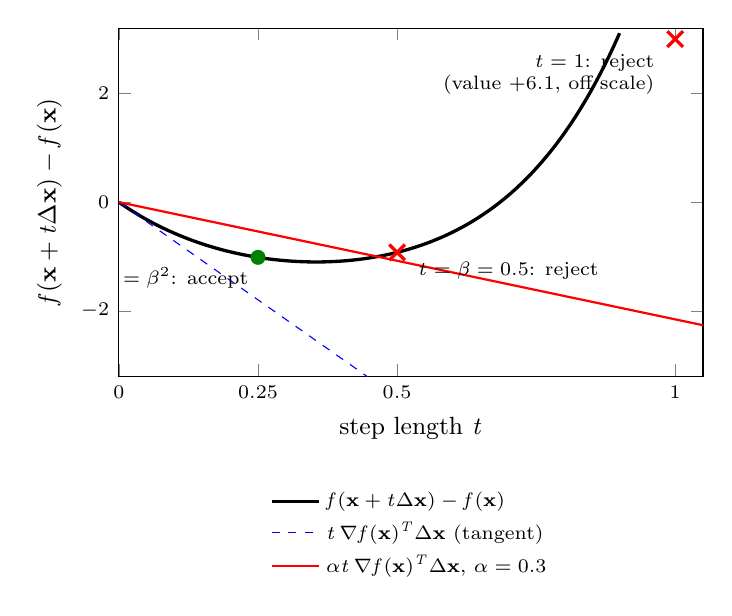
\begin{tikzpicture}
      \begin{axis}[width=9cm, height=6cm, xmin=0, xmax=1.05, ymin=-3.2, ymax=3.2, xlabel={step length $t$},
          ylabel={$f(\vect x+t\Delta\vect x)-f(\vect x)$}, tick label style={font=\scriptsize}, label style={font=\small},
          xtick={0,0.25,0.5,1}, legend style={font=\scriptsize, at={(0.5,-0.3)}, anchor=north, draw=none}, legend columns=1, legend cell align=left, clip=true]
        \addplot[name path=phi, black, very thick] coordinates {(0.0000,0.0000) (0.0088,-0.0621) (0.0176,-0.1218) (0.0265,-0.1791) (0.0353,-0.2341) (0.0441,-0.2868) (0.0529,-0.3374) (0.0618,-0.3859) (0.0706,-0.4323) (0.0794,-0.4768) (0.0882,-0.5194) (0.0971,-0.5601) (0.1059,-0.5990) (0.1147,-0.6361) (0.1235,-0.6716) (0.1324,-0.7054) (0.1412,-0.7376) (0.1500,-0.7682) (0.1588,-0.7973) (0.1676,-0.8248) (0.1765,-0.8510) (0.1853,-0.8756) (0.1941,-0.8989) (0.2029,-0.9208) (0.2118,-0.9414) (0.2206,-0.9606) (0.2294,-0.9785) (0.2382,-0.9951) (0.2471,-1.0105) (0.2559,-1.0246) (0.2647,-1.0375) (0.2735,-1.0492) (0.2824,-1.0596) (0.2912,-1.0688) (0.3000,-1.0768) (0.3088,-1.0837) (0.3176,-1.0893) (0.3265,-1.0937) (0.3353,-1.0970) (0.3441,-1.0990) (0.3529,-1.0999) (0.3618,-1.0995) (0.3706,-1.0979) (0.3794,-1.0951) (0.3882,-1.0910) (0.3971,-1.0857) (0.4059,-1.0791) (0.4147,-1.0713) (0.4235,-1.0621) (0.4324,-1.0515) (0.4412,-1.0397) (0.4500,-1.0264) (0.4588,-1.0117) (0.4676,-0.9956) (0.4765,-0.9780) (0.4853,-0.9588) (0.4941,-0.9382) (0.5029,-0.9159) (0.5118,-0.8920) (0.5206,-0.8664) (0.5294,-0.8390) (0.5382,-0.8099) (0.5471,-0.7789) (0.5559,-0.7460) (0.5647,-0.7112) (0.5735,-0.6744) (0.5824,-0.6354) (0.5912,-0.5943) (0.6000,-0.5509) (0.6088,-0.5052) (0.6176,-0.4572) (0.6265,-0.4066) (0.6353,-0.3535) (0.6441,-0.2977) (0.6529,-0.2391) (0.6618,-0.1776) (0.6706,-0.1132) (0.6794,-0.0457) (0.6882,0.0251) (0.6971,0.0992) (0.7059,0.1767) (0.7147,0.2579) (0.7235,0.3428) (0.7324,0.4316) (0.7412,0.5244) (0.7500,0.6214) (0.7588,0.7228) (0.7676,0.8288) (0.7765,0.9395) (0.7853,1.0551) (0.7941,1.1758) (0.8029,1.3018) (0.8118,1.4334) (0.8206,1.5708) (0.8294,1.7141) (0.8382,1.8637) (0.8471,2.0198) (0.8559,2.1827) (0.8647,2.3526) (0.8735,2.5298) (0.8824,2.7147) (0.8912,2.9075) (0.9000,3.1086)};
        \addlegendentry{$f(\vect x+t\Delta\vect x)-f(\vect x)$}
        \addplot[blue, dashed, domain=0:1.05] {-7.1860*x};
        \addlegendentry{$t\,\nabla f(\vect x)^T\Delta\vect x$ (tangent)}
        \addplot[red, thick, domain=0:1.05] {-2.1558*x};
        \addlegendentry{$\alpha t\,\nabla f(\vect x)^T\Delta\vect x$, $\alpha=0.3$}
        \addplot[only marks, mark=x, mark size=4pt, very thick, red] coordinates {(1,3.0) (0.5,-0.923)};
        \addplot[only marks, mark=*, mark size=2.5pt, green!50!black] coordinates {(0.25,-1.015)};
        \node[font=\scriptsize, anchor=north east, align=right] at (axis cs:0.98,2.9) {$t=1$: reject\\(value $+6.1$, off scale)};
        \node[font=\scriptsize, anchor=north west] at (axis cs:0.52,-0.923) {$t=\beta=0.5$: reject};
        \node[font=\scriptsize, anchor=north east] at (axis cs:0.25,-1.015) {$t=\beta^2$: accept};
      \end{axis}
    \end{tikzpicture}
    \caption{Backtracking (Armijo) line search along a descent direction $\Delta\vect x$. The step $t$ is accepted as soon as the function value lies below the red line $f(\vect x)+\alpha t\nabla f(\vect x)^T\Delta\vect x$, i.\,e.\ as soon as a fraction $\alpha$ of the decrease predicted by the linear approximation (blue, dashed) is actually achieved. Starting with $t=1$, the step is multiplied by $\beta$ until this \emph{sufficient decrease condition} holds. Here $t=1$ even increases $f$ (by about $6.1$, off scale) and $t=0.5$ decreases it too little, so the line search returns $t=\beta^2=0.25$.}
    \label{fig:armijo}
  \end{figure}
 
\subsection{Gradient Descent Methods}
 The most commonly used in machine learning. important to understand how this works. A natural choice of the search direction is the   \textbf{negative gradient}:
  
  \begin{displaymath}
    \Delta \vect x^{(k)} = -\nabla f(\vect x^{(k)})
  \end{displaymath}
\textbf{Rule of thumb:} The negative gradient is the steepest descent direction.

  \begin{algorithmic}
    \STATE \textbf{Input:} function $f$, initial estimate $\vect x^{(0)}$\\
    \STATE initialize: $k:=0$\\
    \Repeat
      \STATE Set descent direction: $\Delta\vect x^{(k)}=- \nabla f(\vect x^{(k)}) $\\
      \STATE Line search (1-D optimization): $t^{(k)}= \argmin_{t \geq 0}f(\vect x^{(k)}+t\cdot \Delta\vect x^{(k)})$\\
      \STATE Update:
        \begin{displaymath}
          \vect x^{(k+1)} = \vect x^{(k)} + t^{(k)}\Delta \vect x^{(k)} .
        \end{displaymath}
      \STATE $k:= k+1$\\
    \Until{$\|\vect x^{(k)} - \vect x^{(k-1)}\|_2 < \epsilon$}\\
    \STATE \textbf{Output:} $\vect x^{(k)}$\\
  \end{algorithmic}
 
\subsection{Steepest Descent Methods}

\subsubsection{Algorithm}
\textbf{(Normalized) steepest descent, what does it mean?} \\
We search for the unit vector that shows the largest decrease in the linear approximation of $f$:
\begin{displaymath}
  \Delta \vect x = \argmin_{\vect u} \{\nabla f(\vect x)^T \vect u ; \ \| \vect u\| = 1\}
\end{displaymath}
for a chosen norm $\|\cdot\|$ (e.\,g.\ $L_1$, $L_2$, $L_\infty$, or the quadratic norm $\|\cdot\|_{\mat P}$).

\textbf{Conclusions:}
  \begin{itemize}
    \item The steepest descent direction depends on the chosen norm.
    \item The negative gradient is not necessarily the best choice for the search direction.
  \end{itemize}
  Figure~\ref{fig:steepest_descent} shows the steepest descent direction for the same gradient and four different norms.

  \begin{figure}[htbp]
    \centering
    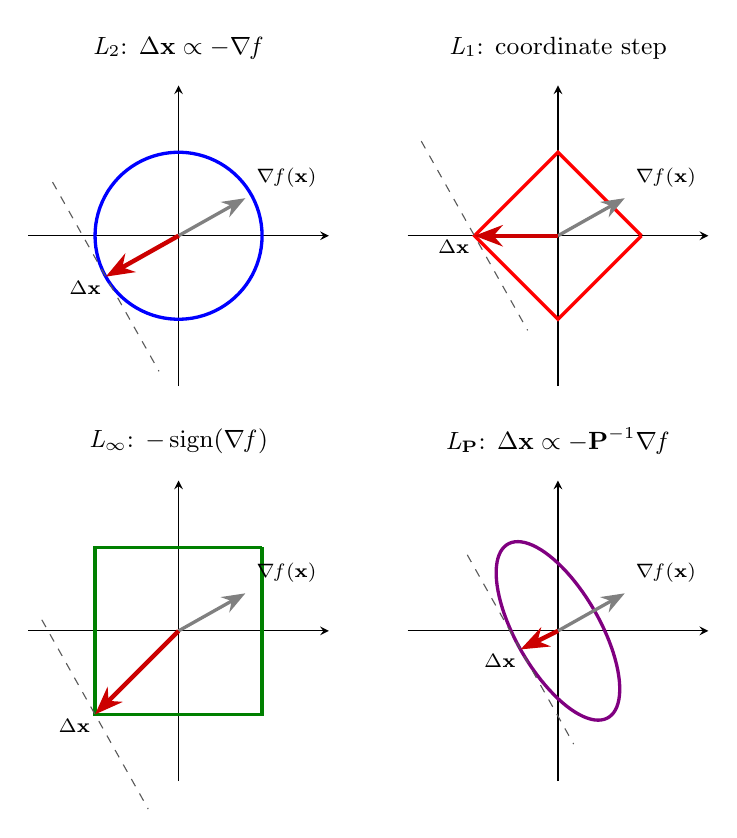
\begin{tikzpicture}[>={Stealth}]
      \begin{groupplot}[group style={group size=2 by 2, horizontal sep=1.0cm, vertical sep=1.2cm}, width=5.4cm, height=5.4cm,
          axis equal image, axis lines=middle, xmin=-1.8, xmax=1.8, ymin=-1.8, ymax=1.8, xtick=\empty, ytick=\empty,
          title style={font=\small}, clip=false]
        \nextgroupplot[title={$L_2$: $\Delta\vect x\propto-\nabla f$}]
          \addplot[blue, very thick, domain=0:360, samples=91, variable=\t] ({cos(\t)}, {sin(\t)});
          \draw[->, very thick, gray] (axis cs:0,0) -- (axis cs:0.8,0.45) node[above right, font=\scriptsize, black] {$\nabla f(\vect x)$};
          \draw[dashed, gray!70!black] (axis cs:-1.509,0.643) -- (axis cs:-0.234,-1.623);
          \draw[->, ultra thick, red!80!black] (axis cs:0,0) -- (axis cs:-0.872,-0.49) node[pos=1.0, below left, font=\scriptsize, black, fill=white, inner sep=1pt] {$\Delta\vect x$};
        \nextgroupplot[title={$L_1$: coordinate step}]
          \addplot[red, very thick] coordinates {(1,0) (0,1) (-1,0) (0,-1) (1,0)};
          \draw[->, very thick, gray] (axis cs:0,0) -- (axis cs:0.8,0.45) node[above right, font=\scriptsize, black] {$\nabla f(\vect x)$};
          \draw[dashed, gray!70!black] (axis cs:-1.637,1.133) -- (axis cs:-0.363,-1.133);
          \draw[->, ultra thick, red!80!black] (axis cs:0,0) -- (axis cs:-1,0) node[pos=1.0, below left, font=\scriptsize, black, fill=white, inner sep=1pt] {$\Delta\vect x$};
        \nextgroupplot[title={$L_\infty$: $-\sign(\nabla f)$}]
          \addplot[green!50!black, very thick] coordinates {(1,1) (-1,1) (-1,-1) (1,-1) (1,1)};
          \draw[->, very thick, gray] (axis cs:0,0) -- (axis cs:0.8,0.45) node[above right, font=\scriptsize, black] {$\nabla f(\vect x)$};
          \draw[dashed, gray!70!black] (axis cs:-1.637,0.133) -- (axis cs:-0.363,-2.133);
          \draw[->, ultra thick, red!80!black] (axis cs:0,0) -- (axis cs:-1,-1) node[pos=1.0, below left, font=\scriptsize, black, fill=white, inner sep=1pt] {$\Delta\vect x$};
        \nextgroupplot[title={$L_{\mat P}$: $\Delta\vect x\propto-\mat P^{-1}\nabla f$}]
          \addplot[violet, very thick, domain=0:360, samples=91, variable=\t] ({0.5*cos(\t)*cos(30)-1.2*sin(\t)*sin(30)}, {0.5*cos(\t)*sin(30)+1.2*sin(\t)*cos(30)});
          \draw[->, very thick, gray] (axis cs:0,0) -- (axis cs:0.8,0.45) node[above right, font=\scriptsize, black] {$\nabla f(\vect x)$};
          \draw[dashed, gray!70!black] (axis cs:-1.086,0.911) -- (axis cs:0.188,-1.355);
          \draw[->, ultra thick, red!80!black] (axis cs:0,0) -- (axis cs:-0.449,-0.222) node[pos=1.0, below left, font=\scriptsize, black, fill=white, inner sep=1pt] {$\Delta\vect x$};
      \end{groupplot}
    \end{tikzpicture}
    \caption{Normalized steepest descent direction $\Delta\vect x=\argmin_{\vect u}\{\nabla f(\vect x)^T\vect u;\ \|\vect u\|=1\}$ for the same gradient $\nabla f(\vect x)$ (gray) and four different norms. The unit ball of each norm is drawn around the current point $\vect x$ (origin). $\Delta\vect x$ (red) is the point of the ball that lies farthest in the direction of $-\nabla f$, i.\,e.\ where a line perpendicular to the gradient (dashed) touches the ball. For $L_2$ this is the negative gradient direction. For $L_1$ it is the corner on the axis of the largest gradient component (coordinate descent). For $L_\infty$ it is a corner of the square ($-\sign(\nabla f)$). For a quadratic norm it is $-\mat P^{-1}\nabla f$, rescaled to the ellipse.}
    \label{fig:steepest_descent}
  \end{figure}
  We consider now the first order Taylor approximation of $f(\vect x +\vect u)$ around the selected position $\vect x$:
  \begin{displaymath}
    f(\vect x+\vect u) \approx f(\vect x) + \nabla f(\vect x)^T \vect u.
  \end{displaymath}
  \begin{itemize}
    \item Here $ \nabla f(\vect x)^T \vect u$ is the directional derivative at $\vect x$ in direction $\vect u$.
    \item The vector $\vect u$ denotes a descent direction if the inner product with the gradient vector is negative, i.\,e.
      \begin{displaymath}
        \nabla f(\vect x)^T \vect u < 0~.
      \end{displaymath}
  \end{itemize}
 
  \begin{algorithmic}
    \STATE \textbf{Input:} function $f$, initial estimate $\vect x^{(0)}$, norm $\|.\|$\\
    \STATE initialize: $k:=0$\\
    \Repeat
      \STATE Compute highest descent direction: $\Delta \vect x ^{(k)}= \argmin_{\vect u} \{\nabla f(\vect x^{(k)})^T \vect u ; \ \| \vect u\| = 1\}$\\
      \STATE Line search (1-D optimization): $t^{(k)}= \argmin_{t \geq 0}f(\vect x^{(k)}+t\cdot \Delta\vect x^{(k)})$\\
      \STATE Update:
        \begin{displaymath}
          \vect x^{(k+1)} = \vect x^{(k)} + t^{(k)}\Delta \vect x^{(k)} .
        \end{displaymath}
      \STATE $k:=k+1$\\
    \Until{$\|\vect x^{(k)} - \vect x^{(k-1)}\| < \epsilon$}\\
    \STATE \textbf{Output:} $\vect x^{(k)}$\\
  \end{algorithmic}
 
\subsubsection{\texorpdfstring{$L_2$}{L2}-norm}
  For the $L_2$-norm the steepest descent direction is the direction of the negative gradient:
  \begin{displaymath}
    \Delta \vect x
    = \argmin_{\vect u} \{\nabla f(\vect x)^T \vect u ; \ \| \vect u\|_2 = 1\}
    = -\frac{\nabla f(\vect x)}{\|\nabla f(\vect x)\|_2}
  \end{displaymath}
  {\small (In practice the unnormalized $\Delta\vect x = -\nabla f(\vect x)$ is used; the line search adapts the step length.)}

\subsubsection{\texorpdfstring{$L_1$}{L1}-norm}

  The unit ball for the $L_1$-norm is a diamond (Figs.~\ref{fig:unitballs} and~\ref{fig:steepest_descent}).
   \begin{itemize}
    \item The steepest descent for the $L_1$-norm selects in each iteration 
      the component of $\nabla f(\vect x)$ with maximum absolute value and then 
      decreases or increases dependent on the sign of the selected component.   
    \item Let $i$ be the index of the gradient component with maximum absolute 
      value, and let $\vect e_i\in\real^d$ denote the corresponding base vector.
      The steepest descent direction is given by:
      \begin{eqnarray*}
        \Delta \vect x &=& \argmin_{\vect u} \{\nabla f(\vect x)^T \vect u ; \ \| \vect u\|_1 = 1\} \\
                      &=& -\sign\left(\frac{\partial}{\partial x_i} f(\vect x)\right)\vect e_i
      \end{eqnarray*}
        
    \item  \textbf{Note:} Steepest descent using the $L_1$-norm results in the {\em coordinate descent algorithm}.
  \end{itemize}
   
\subsubsection{\texorpdfstring{$L_\infty$}{L-infinity}-norm}

  The unit ball for the $L_\infty$-norm is a (hyper)cube (Figs.~\ref{fig:unitballs} and~\ref{fig:steepest_descent}). The steepest descent direction moves every component by the same amount against the sign of its partial derivative:
  \begin{displaymath}
    \Delta \vect x = \argmin_{\vect u} \{\nabla f(\vect x)^T \vect u ; \ \| \vect u\|_\infty = 1\}
    = -\,\sign\big(\nabla f(\vect x)\big) \quad\text{(componentwise)}.
  \end{displaymath}
  
\subsubsection{Quadratic norm \texorpdfstring{$\|\cdot\|_{\mat P}$}{quadratic norm}}

The unit ball for the quadratic norm $\|\vect u\|_{\mat P} = (\vect u^T\mat P\vect u)^{\frac{1}{2}}$, where $\mat P\in\real^{d\times d}$ is symmetric positive definite.

The \textbf{steepest descent} for the norm $\|\cdot\|_{\mat P}$ is given by:
\begin{eqnarray*}
  \Delta \vect x
    &=& \argmin_{\vect u} \{\nabla f(\vect x)^T \vect u ; \ \| \vect u\|_{\mat P} = 1\} \\   
    &=& \argmin_{\vect u} \{\nabla f(\vect x)^T \vect u ;\  (\vect u^T{\mat P}\vect u)^{\frac{1}{2}} = 1\} \\   
    &=& \argmin_{\vect u} \{\nabla f(\vect x)^T \vect u ;\ \| {\mat P}^{\frac{1}{2}} \vect u\|_2 = 1\}~.
\end{eqnarray*}

As we did in the LDA transform, we introduce a change of variables that makes the unit ball \textbf{spherical}:
\begin{displaymath}
  \vect x' = {\mat P}^{\frac{1}{2}} \vect x, \qquad \vect u' = {\mat P}^{\frac{1}{2}} \vect u \quad (\mbox{thus } \|\vect u\|_{\mat P} = \|\vect u'\|_2)
\end{displaymath}

and define the transformed objective
\begin{displaymath}
  f'(\vect x') = f({\mat P}^{-\frac{1}{2}}\vect x') = f(\vect x)~.
\end{displaymath}

Instead of $f(\vect x)$ we now minimize $f'(\vect x')$ using the $L_2$-norm and back-transform the result:
\begin{eqnarray*}
  \Delta \vect x'
    &=& \argmin_{\vect u'} \{\nabla f'(\vect x')^T \vect u' ; \ \| \vect u'\|_{2} = 1\} \\[.15cm]
    &\propto& -\nabla f'(\vect x') \\[.15cm]
    &=& -\mat P^{-\frac{1}{2}}\nabla f({\mat P}^{-\frac{1}{2}}\vect x') \\[.15cm]
    &=& - {\mat P}^{-\frac{1}{2}}\nabla f(\vect x)
\end{eqnarray*}
{\small $\propto$: equal up to a positive scale factor (the normalization), which is absorbed by the line search.}

Now we get for $\Delta \vect x$:
\begin{eqnarray*}
  \Delta \vect x
    &=& {\mat P}^{-\frac{1}{2}} \Delta \vect x' \\[.15cm]
    &\propto& {\mat P}^{-\frac{1}{2}} \left( - {\mat P}^{-\frac{1}{2}}\nabla f(\vect x) \right) \\[.15cm]
    &=& - \mat{P}^{-1} \nabla f(\vect x)~.
\end{eqnarray*}

\textbf{Conclusion:} The (unnormalized) steepest descent direction for the norm $\|\cdot\|_{\mat P}$ is
\begin{displaymath}
   \Delta \vect x = -\mat{P}^{-1} \nabla f(\vect x)~.
\end{displaymath}

\subsection{Newton's Method}
   \textbf{The idea:}
  \begin{itemize}
    \item Select a point.
    \item Compute the minimum of the second order Taylor approximation.
  \end{itemize}
 Second order Taylor approximation:
  \begin{displaymath}
    f(\vect x+\Delta \vect x) 
    \approx f(\vect x) + \nabla f(\vect x)^T \Delta \vect x + \frac{1}{2} \Delta \vect x^T (\nabla^2 f(\vect x))\Delta \vect x 
  \end{displaymath}
  Now we select $\Delta \vect x$ such that 
  \begin{displaymath}
    \nabla\{  f(\vect x) + \nabla f(\vect x)^T \Delta \vect x + \frac{1}{2}\Delta \vect x^T (\nabla^2 f(\vect x))\Delta \vect x\} 
    = 0
  \end{displaymath}
  Obviously the gradient is
  \begin{displaymath}
    \nabla f(\vect x)+ \nabla^2 f(\vect x)\Delta \vect x 
    = 0
  \end{displaymath}
  and thus
  \begin{displaymath}
    \Delta \vect x 
    = -(\nabla^2 f(\vect x))^{-1} \nabla f(\vect x)
  \end{displaymath} 
\textbf{Conclusion:} \\
  Newton's method is an $\vect x$-dependent steepest descent method regarding the quadratic norm $\|\cdot\|_{\mat P}$, where $\mat P = \nabla^2 f(\vect x)$ is the Hessian (assumed positive definite).
  Figure~\ref{fig:gd_vs_newton} compares gradient descent and Newton's method on a 2-D example.

  \begin{figure}[htbp]
    \centering
    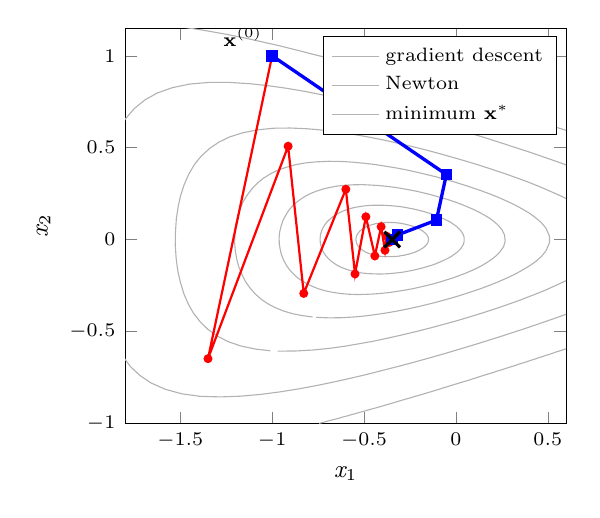
\begin{tikzpicture}
      \begin{axis}[width=8.6cm, height=6.6cm, xmin=-1.8, xmax=0.6, ymin=-1.0, ymax=1.15, axis equal image,
          xlabel={$x_1$}, ylabel={$x_2$}, tick label style={font=\scriptsize}, label style={font=\small},
          legend style={font=\scriptsize, at={(0.98,0.98)}, anchor=north east}, legend cell align=left]
\addplot[gray!60, thin] coordinates {(-0.410,-0.091) (-0.411,-0.091) (-0.420,-0.089) (-0.430,-0.088) (-0.440,-0.086) (-0.450,-0.083) (-0.450,-0.083) (-0.460,-0.080) (-0.470,-0.077) (-0.473,-0.076) (-0.480,-0.073) (-0.490,-0.069) (-0.490,-0.069) (-0.500,-0.063) (-0.503,-0.061) (-0.510,-0.057) (-0.513,-0.054) (-0.520,-0.048) (-0.522,-0.047) (-0.529,-0.039) (-0.530,-0.038) (-0.534,-0.032) (-0.538,-0.025) (-0.540,-0.020) (-0.541,-0.017) (-0.543,-0.010) (-0.544,-0.003) (-0.544,0.005) (-0.543,0.012) (-0.540,0.019) (-0.540,0.020) (-0.537,0.027) (-0.533,0.034) (-0.530,0.038) (-0.527,0.041) (-0.520,0.049) (-0.520,0.049) (-0.511,0.056) (-0.510,0.057) (-0.500,0.063) (-0.500,0.063) (-0.490,0.069) (-0.486,0.071) (-0.480,0.073) (-0.470,0.077) (-0.468,0.078) (-0.460,0.080) (-0.450,0.083) (-0.442,0.085) (-0.440,0.086) (-0.430,0.088) (-0.420,0.089) (-0.410,0.091) (-0.400,0.092) (-0.390,0.093) (-0.389,0.093) (-0.380,0.093) (-0.370,0.093) (-0.360,0.093) (-0.350,0.093) (-0.343,0.093) (-0.340,0.093) (-0.330,0.092) (-0.320,0.091) (-0.310,0.090) (-0.300,0.088) (-0.290,0.087) (-0.284,0.085) (-0.280,0.085) (-0.270,0.082) (-0.260,0.080) (-0.253,0.078) (-0.250,0.077) (-0.240,0.074) (-0.230,0.071) (-0.230,0.071) (-0.220,0.067) (-0.211,0.063) (-0.210,0.063) (-0.200,0.058) (-0.196,0.056) (-0.190,0.052) (-0.184,0.049) (-0.180,0.046) (-0.174,0.041) (-0.170,0.038) (-0.166,0.034) (-0.160,0.028) (-0.159,0.027) (-0.154,0.019) (-0.151,0.012) (-0.150,0.007) (-0.150,0.005) (-0.149,-0.003) (-0.150,-0.007) (-0.151,-0.010) (-0.153,-0.017) (-0.158,-0.025) (-0.160,-0.027) (-0.164,-0.032) (-0.170,-0.038) (-0.171,-0.039) (-0.180,-0.046) (-0.181,-0.047) (-0.190,-0.052) (-0.193,-0.054) (-0.200,-0.058) (-0.207,-0.061) (-0.210,-0.063) (-0.220,-0.067) (-0.224,-0.069) (-0.230,-0.071) (-0.240,-0.074) (-0.246,-0.076) (-0.250,-0.077) (-0.260,-0.080) (-0.270,-0.082) (-0.274,-0.083) (-0.280,-0.085) (-0.290,-0.086) (-0.300,-0.088) (-0.310,-0.090) (-0.319,-0.091) (-0.320,-0.091) (-0.330,-0.092) (-0.340,-0.092) (-0.350,-0.093) (-0.360,-0.093) (-0.370,-0.093) (-0.380,-0.093) (-0.390,-0.093) (-0.400,-0.092) (-0.410,-0.091)};
\addplot[gray!60, thin] coordinates {(-0.460,-0.186) (-0.480,-0.185) (-0.510,-0.182) (-0.530,-0.179) (-0.560,-0.172) (-0.580,-0.167) (-0.600,-0.160) (-0.620,-0.153) (-0.640,-0.143) (-0.654,-0.135) (-0.670,-0.124) (-0.684,-0.113) (-0.699,-0.098) (-0.710,-0.085) (-0.720,-0.070) (-0.728,-0.054) (-0.733,-0.039) (-0.738,-0.017) (-0.739,0.005) (-0.737,0.027) (-0.730,0.049) (-0.724,0.063) (-0.715,0.078) (-0.704,0.093) (-0.690,0.107) (-0.680,0.116) (-0.663,0.129) (-0.650,0.137) (-0.630,0.148) (-0.610,0.157) (-0.590,0.164) (-0.570,0.170) (-0.550,0.175) (-0.520,0.180) (-0.500,0.183) (-0.470,0.186) (-0.440,0.187) (-0.410,0.187) (-0.380,0.186) (-0.350,0.184) (-0.320,0.181) (-0.300,0.179) (-0.270,0.174) (-0.250,0.170) (-0.229,0.166) (-0.200,0.159) (-0.180,0.154) (-0.160,0.148) (-0.140,0.142) (-0.120,0.135) (-0.100,0.128) (-0.080,0.119) (-0.060,0.110) (-0.040,0.100) (-0.027,0.093) (-0.010,0.081) (0.004,0.071) (0.020,0.056) (0.030,0.044) (0.040,0.027) (0.045,0.012) (0.045,-0.010) (0.040,-0.027) (0.030,-0.044) (0.020,-0.056) (0.006,-0.069) (-0.010,-0.081) (-0.024,-0.091) (-0.040,-0.100) (-0.060,-0.110) (-0.080,-0.119) (-0.099,-0.127) (-0.118,-0.135) (-0.140,-0.142) (-0.160,-0.148) (-0.180,-0.154) (-0.200,-0.159) (-0.220,-0.164) (-0.250,-0.170) (-0.270,-0.174) (-0.300,-0.179) (-0.320,-0.181) (-0.350,-0.184) (-0.373,-0.186) (-0.400,-0.187) (-0.430,-0.187) (-0.460,-0.186)};
\addplot[gray!60, thin] coordinates {(-0.590,-0.297) (-0.630,-0.293) (-0.670,-0.287) (-0.710,-0.279) (-0.750,-0.267) (-0.780,-0.255) (-0.810,-0.241) (-0.840,-0.223) (-0.861,-0.208) (-0.885,-0.186) (-0.905,-0.164) (-0.921,-0.142) (-0.937,-0.113) (-0.949,-0.083) (-0.956,-0.054) (-0.961,-0.025) (-0.962,0.012) (-0.959,0.041) (-0.950,0.078) (-0.940,0.106) (-0.928,0.129) (-0.910,0.158) (-0.891,0.181) (-0.870,0.200) (-0.849,0.217) (-0.820,0.236) (-0.790,0.251) (-0.760,0.263) (-0.720,0.276) (-0.689,0.283) (-0.647,0.291) (-0.600,0.296) (-0.560,0.298) (-0.510,0.299) (-0.470,0.297) (-0.420,0.294) (-0.380,0.290) (-0.330,0.284) (-0.290,0.277) (-0.250,0.270) (-0.210,0.262) (-0.176,0.254) (-0.140,0.245) (-0.100,0.234) (-0.067,0.225) (-0.030,0.213) (0.000,0.203) (0.039,0.188) (0.070,0.175) (0.100,0.162) (0.130,0.147) (0.160,0.130) (0.185,0.115) (0.210,0.096) (0.230,0.078) (0.250,0.054) (0.264,0.027) (0.268,-0.010) (0.259,-0.039) (0.240,-0.067) (0.220,-0.087) (0.198,-0.105) (0.170,-0.124) (0.140,-0.142) (0.111,-0.157) (0.080,-0.171) (0.050,-0.184) (0.020,-0.195) (-0.015,-0.208) (-0.050,-0.219) (-0.085,-0.230) (-0.120,-0.240) (-0.160,-0.250) (-0.199,-0.259) (-0.233,-0.267) (-0.272,-0.274) (-0.316,-0.281) (-0.360,-0.288) (-0.400,-0.292) (-0.447,-0.296) (-0.490,-0.298) (-0.540,-0.299) (-0.590,-0.297)};
\addplot[gray!60, thin] coordinates {(-0.780,-0.421) (-0.840,-0.413) (-0.890,-0.403) (-0.940,-0.388) (-0.986,-0.369) (-1.027,-0.347) (-1.060,-0.324) (-1.092,-0.296) (-1.120,-0.264) (-1.144,-0.230) (-1.163,-0.193) (-1.180,-0.152) (-1.191,-0.113) (-1.200,-0.064) (-1.204,-0.017) (-1.203,0.034) (-1.198,0.078) (-1.189,0.122) (-1.175,0.166) (-1.159,0.203) (-1.138,0.239) (-1.110,0.276) (-1.082,0.305) (-1.050,0.332) (-1.011,0.357) (-0.970,0.377) (-0.924,0.393) (-0.870,0.408) (-0.820,0.417) (-0.760,0.423) (-0.690,0.426) (-0.620,0.425) (-0.560,0.421) (-0.497,0.415) (-0.438,0.408) (-0.380,0.399) (-0.320,0.389) (-0.269,0.379) (-0.210,0.366) (-0.160,0.354) (-0.110,0.342) (-0.057,0.327) (-0.007,0.313) (0.041,0.298) (0.090,0.282) (0.140,0.265) (0.188,0.247) (0.230,0.230) (0.275,0.210) (0.320,0.189) (0.360,0.167) (0.399,0.144) (0.430,0.122) (0.464,0.093) (0.490,0.062) (0.509,0.019) (0.509,-0.017) (0.490,-0.061) (0.466,-0.091) (0.433,-0.120) (0.400,-0.143) (0.360,-0.167) (0.320,-0.189) (0.280,-0.208) (0.230,-0.230) (0.190,-0.246) (0.140,-0.265) (0.092,-0.281) (0.047,-0.296) (0.000,-0.311) (-0.050,-0.325) (-0.104,-0.340) (-0.160,-0.354) (-0.210,-0.366) (-0.260,-0.377) (-0.320,-0.389) (-0.377,-0.399) (-0.430,-0.407) (-0.490,-0.415) (-0.552,-0.421) (-0.620,-0.425) (-0.690,-0.426) (-0.760,-0.423)};
\addplot[gray!60, thin] coordinates {(-1.010,-0.605) (-1.090,-0.596) (-1.170,-0.579) (-1.240,-0.555) (-1.300,-0.524) (-1.350,-0.488) (-1.390,-0.449) (-1.429,-0.399) (-1.458,-0.347) (-1.480,-0.295) (-1.500,-0.230) (-1.513,-0.171) (-1.522,-0.105) (-1.527,-0.032) (-1.526,0.041) (-1.521,0.115) (-1.511,0.181) (-1.498,0.239) (-1.479,0.298) (-1.453,0.357) (-1.423,0.408) (-1.388,0.452) (-1.340,0.496) (-1.290,0.530) (-1.230,0.559) (-1.160,0.581) (-1.080,0.597) (-0.990,0.606) (-0.900,0.607) (-0.810,0.603) (-0.720,0.595) (-0.632,0.584) (-0.550,0.571) (-0.470,0.557) (-0.390,0.541) (-0.320,0.525) (-0.240,0.507) (-0.168,0.489) (-0.090,0.468) (-0.020,0.448) (0.050,0.428) (0.120,0.407) (0.190,0.384) (0.260,0.361) (0.330,0.336) (0.393,0.313) (0.460,0.286) (0.520,0.260) (0.582,0.232) (0.640,0.202) (0.700,0.167) (0.750,0.131) (0.792,0.093) (0.825,0.041) (0.831,-0.025) (0.805,-0.076) (0.764,-0.120) (0.715,-0.157) (0.660,-0.191) (0.600,-0.223) (0.540,-0.251) (0.480,-0.278) (0.417,-0.303) (0.350,-0.329) (0.280,-0.354) (0.213,-0.377) (0.145,-0.399) (0.074,-0.421) (0.000,-0.443) (-0.070,-0.462) (-0.140,-0.481) (-0.219,-0.501) (-0.290,-0.518) (-0.370,-0.536) (-0.449,-0.553) (-0.528,-0.567) (-0.610,-0.581) (-0.690,-0.592) (-0.780,-0.601) (-0.870,-0.606) (-0.970,-0.607)};
\addplot[gray!60, thin] coordinates {(1.000,-0.238) (0.926,-0.274) (0.850,-0.308) (0.773,-0.340) (0.698,-0.369) (0.620,-0.399) (0.539,-0.428) (0.455,-0.457) (0.370,-0.486) (0.290,-0.512) (0.209,-0.538) (0.120,-0.566) (0.040,-0.590) (-0.050,-0.617) (-0.134,-0.641) (-0.220,-0.665) (-0.310,-0.689) (-0.400,-0.712) (-0.490,-0.735) (-0.580,-0.756) (-0.670,-0.776) (-0.762,-0.795) (-0.860,-0.813) (-0.960,-0.829) (-1.060,-0.842) (-1.170,-0.852) (-1.280,-0.856) (-1.390,-0.853) (-1.492,-0.839) (-1.580,-0.815) (-1.659,-0.780) (-1.720,-0.739) (-1.770,-0.692) (-1.814,-0.633) (-1.850,-0.567) (-1.876,-0.501) (-1.897,-0.428) (-1.913,-0.355) (-1.925,-0.274) (-1.933,-0.193) (-1.938,-0.105) (-1.940,-0.025) (-1.940,0.056) (-1.936,0.144) (-1.930,0.226) (-1.920,0.309) (-1.906,0.386) (-1.889,0.459) (-1.864,0.533) (-1.834,0.599) (-1.798,0.657) (-1.750,0.713) (-1.692,0.760) (-1.626,0.797) (-1.545,0.826) (-1.450,0.846) (-1.346,0.855) (-1.230,0.855) (-1.120,0.848) (-1.020,0.837) (-0.920,0.823) (-0.820,0.806) (-0.730,0.788) (-0.631,0.767) (-0.540,0.746) (-0.450,0.725) (-0.360,0.702) (-0.274,0.679) (-0.190,0.656) (-0.100,0.631) (-0.014,0.606) (0.070,0.581) (0.156,0.555) (0.240,0.528) (0.320,0.502) (0.406,0.474) (0.490,0.445) (0.570,0.417) (0.650,0.388) (0.730,0.357) (0.804,0.327) (0.880,0.295) (0.953,0.261)};
\addplot[gray!60, thin] coordinates {(1.000,-0.454) (0.980,-0.461) (0.960,-0.468) (0.940,-0.476) (0.920,-0.483) (0.900,-0.490) (0.880,-0.497) (0.860,-0.504) (0.840,-0.511) (0.820,-0.518) (0.800,-0.525) (0.780,-0.532) (0.760,-0.539) (0.740,-0.546) (0.720,-0.553) (0.699,-0.560) (0.678,-0.567) (0.656,-0.575) (0.635,-0.582) (0.613,-0.589) (0.591,-0.597) (0.570,-0.604) (0.550,-0.610) (0.530,-0.617) (0.510,-0.624) (0.490,-0.630) (0.470,-0.637) (0.450,-0.643) (0.430,-0.650) (0.410,-0.656) (0.390,-0.663) (0.368,-0.670) (0.345,-0.677) (0.323,-0.685) (0.300,-0.692) (0.280,-0.698) (0.260,-0.705) (0.240,-0.711) (0.220,-0.717) (0.200,-0.724) (0.180,-0.730) (0.160,-0.736) (0.138,-0.743) (0.114,-0.751) (0.091,-0.758) (0.070,-0.765) (0.050,-0.771) (0.030,-0.777) (0.010,-0.783) (-0.010,-0.789) (-0.030,-0.795) (-0.052,-0.802) (-0.076,-0.809) (-0.100,-0.817) (-0.120,-0.823) (-0.140,-0.829) (-0.160,-0.835) (-0.180,-0.841) (-0.200,-0.847) (-0.222,-0.853) (-0.247,-0.861) (-0.270,-0.867) (-0.290,-0.873) (-0.310,-0.879) (-0.330,-0.885) (-0.350,-0.891) (-0.372,-0.897) (-0.398,-0.905) (-0.420,-0.911) (-0.440,-0.917) (-0.460,-0.922) (-0.480,-0.928) (-0.501,-0.934) (-0.527,-0.941) (-0.550,-0.948) (-0.570,-0.953) (-0.590,-0.959) (-0.610,-0.964) (-0.634,-0.971) (-0.660,-0.978) (-0.680,-0.983) (-0.700,-0.988) (-0.720,-0.994) (-0.744,-1.000)};
\addplot[gray!60, thin] coordinates {(-2.000,1.151) (-1.960,1.160) (-1.920,1.166) (-1.878,1.171) (-1.830,1.174) (-1.780,1.176) (-1.730,1.175) (-1.680,1.173) (-1.635,1.171) (-1.590,1.167) (-1.550,1.163) (-1.500,1.157) (-1.460,1.152) (-1.420,1.146) (-1.380,1.140) (-1.340,1.133) (-1.300,1.126) (-1.260,1.119) (-1.220,1.111) (-1.180,1.103) (-1.140,1.095) (-1.100,1.086) (-1.060,1.077) (-1.020,1.068) (-0.988,1.061) (-0.950,1.052) (-0.910,1.042) (-0.870,1.032) (-0.838,1.024) (-0.800,1.014) (-0.760,1.004) (-0.724,0.995) (-0.690,0.986) (-0.650,0.975) (-0.615,0.965) (-0.580,0.956) (-0.540,0.945) (-0.508,0.936) (-0.470,0.925) (-0.430,0.914) (-0.400,0.905) (-0.360,0.894) (-0.329,0.885) (-0.290,0.873) (-0.254,0.863) (-0.220,0.853) (-0.180,0.841) (-0.150,0.832) (-0.110,0.820) (-0.080,0.811) (-0.040,0.798) (-0.010,0.789) (0.030,0.777) (0.061,0.767) (0.100,0.755) (0.132,0.745) (0.170,0.733) (0.201,0.723) (0.240,0.711) (0.271,0.701) (0.310,0.689) (0.340,0.679) (0.380,0.666) (0.410,0.656) (0.450,0.643) (0.480,0.633) (0.519,0.621) (0.550,0.610) (0.585,0.599) (0.620,0.587) (0.650,0.577) (0.690,0.563) (0.720,0.553) (0.758,0.540) (0.790,0.529) (0.821,0.518) (0.860,0.504) (0.890,0.494) (0.924,0.481) (0.960,0.468) (0.990,0.457)};
        \addplot[red, thick, mark=*, mark size=1.2pt] coordinates {(-1.000,1.000) (-1.349,-0.648) (-0.913,0.508) (-0.828,-0.293) (-0.599,0.274) (-0.549,-0.187) (-0.490,0.124) (-0.441,-0.089) (-0.407,0.070) (-0.386,-0.058) (-0.376,0.018) (-0.364,-0.016) (-0.359,0.005) (-0.354,-0.005) (-0.351,0.004) (-0.349,-0.002) (-0.348,0.001) (-0.348,-0.001) (-0.347,0.000) (-0.347,-0.000) (-0.347,0.000) (-0.347,-0.000) (-0.347,0.000) (-0.347,-0.000) (-0.347,0.000) (-0.347,-0.000)};
        \addlegendentry{gradient descent}
        \addplot[blue, very thick, mark=square*, mark size=1.5pt] coordinates {(-1.000,1.000) (-0.052,0.354) (-0.106,0.106) (-0.318,0.025) (-0.345,0.001) (-0.347,0.000) (-0.347,0.000)};
        \addlegendentry{Newton}
        \addplot[only marks, mark=x, mark size=4pt, very thick, black] coordinates {(-0.3466,0)};
        \addlegendentry{minimum $\vect x^*$}
        \node[font=\scriptsize, anchor=south east] at (axis cs:-1.0,1.0) {$\vect x^{(0)}$};
      \end{axis}
    \end{tikzpicture}
    \caption{Gradient descent vs.\ Newton's method on $f(\vect x)=e^{x_1+3x_2-0.1}+e^{x_1-3x_2-0.1}+e^{-x_1-0.1}$ (example from Boyd and Vandenberghe; gray: contour lines), both with backtracking line search ($\alpha=0.1$, $\beta=0.7$) from $\vect x^{(0)}=(-1,1)^T$. The contours are elongated, so the negative gradient does not point to the minimum and gradient descent zig-zags across the valley: after $10$ iterations the error $f(\vect x^{(k)})-f(\vect x^*)$ is still about $3\cdot10^{-3}$. Newton's method rescales the step with the inverse Hessian (steepest descent in the local quadratic norm $\|\cdot\|_{\nabla^2 f}$) and reaches an error of $10^{-11}$ after $5$ iterations.}
    \label{fig:gd_vs_newton}
  \end{figure}
  
  \subsubsection{Damped Newton's Method}
  
  \begin{algorithmic}
    \STATE \textbf{Input:} function $f$, initial estimate $\vect x^{(0)}$\\
    \STATE initialize: $k:=0$\\
    \Repeat
      \STATE Compute Newton step: $\Delta \vect x^{(k)}= -\big(\nabla^2 f(\vect x^{(k)})\big)^{-1} \nabla f(\vect x^{(k)})$\\
      \STATE Line search (1-D optimization): $t^{(k)}= \argmin_{t \geq 0}f(\vect x^{(k)}+t\cdot \Delta\vect x^{(k)})$\\
      \STATE Update:
        \begin{displaymath}
          \vect x^{(k+1)} = \vect x^{(k)} + t^{(k)}\Delta \vect x^{(k)}
        \end{displaymath}
      \STATE $k:=k+1$\\
    \Until{$\|\vect x^{(k)} - \vect x^{(k-1)}\| < \epsilon$}\\
    \STATE \textbf{Output:} $\vect x^{(k)}$\\
  \end{algorithmic}
 
\subsection{Lessons Learned}

  \begin{itemize}
    \item Gradient descent is widely applied.
    \item Gradient descent and coordinate descent are special cases of steepest descent methods. 
    \item Steepest descent method depends on the chosen norm.
  \end{itemize}

\subsection{Comprehensive Questions}

  \begin{itemize}
    \item What is the general formulation for an unconstrained optimization problem? 
    \item Why do we need a line search in gradient descent approaches? 
    \item What is the Armijo-Goldstein line search algorithm? 
    \item What are the steepest descent directions if we apply the $L_\infty$, $L_1$, $L_2$, and the quadratic norm $\|\cdot\|_{\mat P}$?
  \end{itemize}
Now we make a small deviation into SVMs before continuing with the optimization chapter. It is important to understand SVMs to continue.

\newpage
\section{Support Vector Machines I}

This is an important chapter for the exam.\autocite{vapnik2000,hastie2009,bishop2006,schoelkopf2002}

\subsection{Motivation}

  \begin{itemize}
  \item Assume two linearly separable classes. 
  \item Computation of linear decision boundary that allows the separation of 
    training data and that generalizes well.
  \item Vapnik: Optimal separating hyperplane separates two classes and maximizes the distance to the closest point from either class. This results in
    \begin{itemize}
      \item unique solution for hyperplanes, and
      \item (in most cases) better generalization.
    \end{itemize}
  \end{itemize}
  
  \subsection{Remarks on Linear Algebra}

  Assume we have an affine \textbf{decision function}:
  \begin{eqnarray*}
    f(\vect x) &=& \vect \alpha^T \vect x + \alpha_0
  \end{eqnarray*}
  The \textbf{decision boundary} is the hyperplane $\{\vect x : f(\vect x)=0\}$.
  \begin{itemize}
    \item For any point $\vect x$ on the hyperplane, we have $f(\vect x)= 0$.      
    \item A necessary condition for two points on the hyperplane is:
      \begin{displaymath}
        f(\vect x_1) = f(\vect x_2) \quad \mbox{and thus} \quad \vect \alpha^T (\vect x_1-\vect x_2) =0.
      \end{displaymath}
    \item The  \textbf {normal vector $\vect n$} of the hyperplane is $\vect n= \vect \alpha/\|\vect \alpha\|_2$.

    \item \textbf{Derivation of the signed distance $\delta$} of $\vect x$ to the hyperplane: Let $\vect x_\perp$ be the orthogonal projection of $\vect x$ onto the hyperplane $\{\vect x:f(\vect x)=0\}$.
          Decompose $\vect x$ along the unit normal $\vect n=\vect\alpha/\|\vect\alpha\|_2$:
          {\small
          \[
            \vect x = \vect x_\perp + \delta\,\vect n, \qquad f(\vect x_\perp)=0~.
          \]
          }
          Applying $f(\cdot)=\vect\alpha^T(\cdot)+\alpha_0$ gives
          {\small
          \[
            f(\vect x)=f(\vect x_\perp)+\delta\,\vect\alpha^T\vect n
            = 0 + \delta\,\frac{\vect\alpha^T\vect\alpha}{\|\vect\alpha\|_2}
            = \delta\,\|\vect\alpha\|_2,
            \quad\Rightarrow\quad \delta=\frac{f(\vect x)}{\|\vect\alpha\|_2}~.
          \]
          }

      \begin{displaymath}
        \delta(\vect x) = 
        \frac{\|\vect \alpha\|_2}{\vect \alpha^T\vect \alpha} \cdot f(\vect x) = 
        \frac{1}{\|\vect \alpha\|_2}\cdot f(\vect x)  =
        \frac{1}{\|\nabla f(\vect x)\|_2}\cdot f(\vect x)  
      \end{displaymath}

    \item Assume points $\vect x_1, \vect x_2$ on either side of the margin satisfy $f(\vect x_1)= +1$ and $f(\vect x_2)=-1$. Thus we have:
      \begin{displaymath}
        \vect \alpha^T (\vect x_1 - \vect x_2) = 2 \quad \mbox{and} \quad
        \frac{\vect \alpha^T}{\|\vect \alpha\|_2} (\vect x_1-\vect x_2) 
        = \frac{2}{\|\vect \alpha\|_2}
      \end{displaymath}
      i.\,e.\ the \textbf{margin} (width between the hyperplanes $f(\vect x)=\pm 1$) is $2/\|\vect\alpha\|_2$.
  \end{itemize}
  
\subsection{Hard Margin Problem}

Training set $S=\{(\vect x_i, y_i)\}_{i=1}^m$, $\vect x_i\in\real^d$, with \textbf{labels $y_i\in\{-1,+1\}$}.
The \textbf{predicted label} of a feature vector $\vect x$ is
\begin{displaymath}
  \hat y = \sign(f(\vect x)) = \sign(\vect\alpha^T\vect x+\alpha_0)~.
\end{displaymath}

\textbf{Constraints:}
  \begin{itemize}
    \item Separation of classes has to be done with margin:
      \begin{eqnarray*}
        \vect \alpha^T \vect x_i+\alpha_0 &\leq& -1, \quad \mbox{if} \quad y_i= -1 \\
        \vect \alpha^T \vect x_i+\alpha_0 &\geq& +1, \quad \mbox{if} \quad y_i= +1
      \end{eqnarray*}
    \item This is equivalent to:
      \begin{displaymath}
        y_i\cdot (\vect \alpha^T\vect x_i + \alpha_0) \geq 1
      \end{displaymath}
  \end{itemize}
  \textbf{Functional vs.\ geometric margin:} $y_i(\vect\alpha^T\vect x_i+\alpha_0)$ is the \emph{functional} margin of sample $i$; it changes if $(\vect\alpha,\alpha_0)$ is rescaled. The \emph{geometric} margin $y_i(\vect\alpha^T\vect x_i+\alpha_0)/\|\vect\alpha\|_2$ (signed distance) does not. We can therefore fix the scale by requiring a functional margin of at least $1$ for every sample, without loss of generality; then the geometric margin is $1/\|\vect\alpha\|_2$ on each side.

  The  \textbf{maximization} of the margin $2/\|\vect\alpha\|_2$ corresponds to the following optimization problem with linear constraints:
  \begin{center}
        $\begin{aligned}
           \displaystyle 
           \mbox{maximize}   &\qquad \frac{1}{\|\vect \alpha\|_2} \\
           \mbox{subject to} &\qquad \forall i:~ y_i\cdot (\vect \alpha^T\vect x_i + \alpha_0) \geq 1
        \end{aligned}$
  \end{center}
 \textbf {Note:}
  \begin{itemize}
    \item The linear constraints enforce that every training sample lies at least one margin unit away from the decision boundary; the objective then maximizes that margin.
    \item Basically we compute the distance of the convex hulls of feature sets. 
    \item We need constrained optimization methods to solve the problem.
  \end{itemize}
  The optimization problem is equivalent to 
  \begin{center}
       $\begin{aligned}
           \displaystyle 
           \mbox{minimize}   &\qquad \frac{1}{2} {\|\vect \alpha\|^2_2} \\
           \mbox{subject to} &\qquad \forall i:~ y_i\cdot (\vect \alpha^T\vect x_i + \alpha_0) -1 \geq 0
        \end{aligned}$
   \end{center}
  \textbf {Remarks on the optimization problem:}
  
  \begin{itemize}
    \item Convex optimization problem 
    \item Efficient algorithms for solving the convex optimization problem (interior point method) 
    \item Standard libraries can be used for minimization 
    \item The optimal $\vect\alpha$ is unique (strictly convex objective); for separable data with samples of both classes, $\alpha_0$ is then fixed by the active constraints
  \end{itemize}

\subsection{Soft Margin Problem}

 If classes are not linearly separable, we have to introduce  \textbf {\emph{slack variables}}. \\ 
\textbf {Convex optimization problem:}
  
  \begin{center}
        $\begin{aligned}
           \displaystyle 
           \mbox{minimize}    &\qquad \frac{1}{2} {\|\vect \alpha\|^2_2} + \mu \sum_i \xi_i \\
            \mbox{subject to} &\qquad \forall i:~ -(y_i\cdot (\vect \alpha^T\vect x_i + \alpha_0) -1+\xi_i) \leq 0~,\\
                              &\qquad \forall i:~ -\xi_i \leq 0
        \end{aligned}$
  \end{center}
  
{\small where $\xi_i\geq 0$ is the slack variable of sample $\vect x_i$ (amount of margin violation), and $\mu>0$ is a user-chosen weight (meta-parameter) trading margin width against violations.}
Figure~\ref{fig:svm_margin} shows the geometry of the hard- and the soft-margin solution.

  \begin{figure}[htbp]
    \centering
    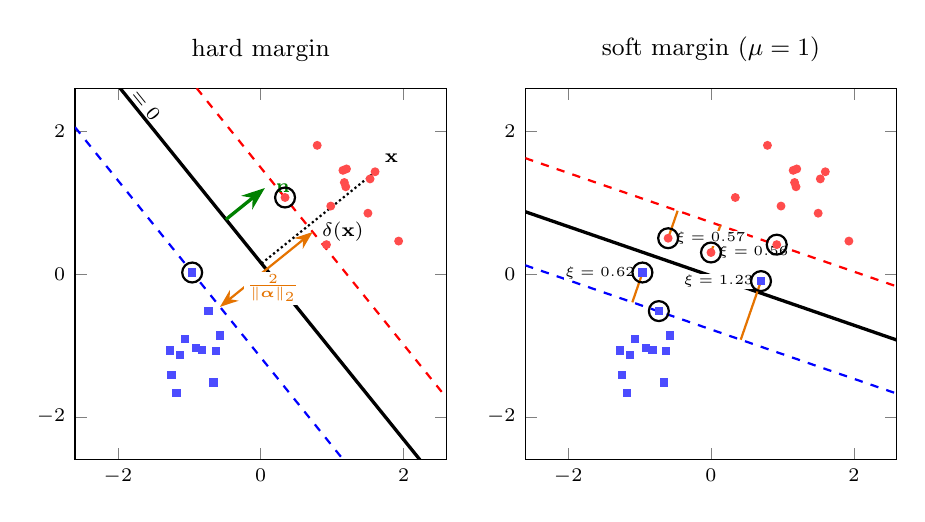
\begin{tikzpicture}
      \begin{groupplot}[group style={group size=2 by 1, horizontal sep=1.0cm}, width=6.3cm, height=6.3cm,
          axis equal image, xmin=-2.6, xmax=2.6, ymin=-2.6, ymax=2.6, xtick={-2,0,2}, ytick={-2,0,2},
          tick label style={font=\scriptsize}, title style={font=\small}]
        \nextgroupplot[title={hard margin}]
\addplot[only marks, mark=*, mark size=1.4pt, red!70] coordinates {(1.20,1.47) (1.53,1.33) (1.93,0.46) (0.92,0.41) (1.15,1.45) (1.19,1.22) (0.34,1.07) (0.79,1.80) (1.60,1.43) (1.17,1.28) (1.50,0.85) (0.98,0.95)};
\addplot[only marks, mark=square*, mark size=1.3pt, blue!70] coordinates {(-1.27,-1.07) (-1.13,-1.13) (-0.66,-1.52) (-0.63,-1.08) (-1.25,-1.41) (-1.06,-0.91) (-0.91,-1.04) (-0.96,0.02) (-0.82,-1.06) (-0.57,-0.86) (-0.73,-0.52) (-1.18,-1.67)};
\addplot[only marks, mark=o, mark size=3.6pt, thick, black] coordinates {(0.34,1.07) (-0.96,0.02)};
\addplot[black, very thick] coordinates {(-1.969,2.600) (2.227,-2.600)};
\addplot[red, dashed, thick] coordinates {(-0.897,2.600) (2.600,-1.734)};
\addplot[blue, dashed, thick] coordinates {(-2.600,2.054) (1.155,-2.600)};
\draw[{Stealth}-{Stealth}, thick, orange!90!black] (axis cs:-0.571,-0.461) -- (axis cs:0.727,0.587) node[pos=0.25, right, font=\scriptsize, fill=white, inner sep=1pt] {$\frac{2}{\|\vect\alpha\|_2}$};
\draw[-{Stealth}, very thick, green!50!black] (axis cs:-0.487,0.763) -- (axis cs:0.058,1.203) node[right, font=\scriptsize] {$\vect n$};
\draw[densely dotted, thick] (axis cs:0.011,0.146) -- (axis cs:1.599,1.427) node[pos=0.5, below right, font=\scriptsize, inner sep=1pt] {$\delta(\vect x)$};
\node[font=\scriptsize, anchor=south west] at (axis cs:1.599,1.427) {$\vect x$};
\node[font=\scriptsize, rotate=-51.1] at (axis cs:-1.7,2.447) {$f=0$};

        \nextgroupplot[title={soft margin ($\mu=1$)}]
\addplot[only marks, mark=*, mark size=1.4pt, red!70] coordinates {(1.20,1.47) (1.53,1.33) (1.93,0.46) (0.92,0.41) (1.15,1.45) (1.19,1.22) (0.34,1.07) (0.79,1.80) (1.60,1.43) (1.17,1.28) (1.50,0.85) (0.98,0.95) (0.00,0.30) (-0.60,0.50)};
\addplot[only marks, mark=square*, mark size=1.3pt, blue!70] coordinates {(-1.27,-1.07) (-1.13,-1.13) (-0.66,-1.52) (-0.63,-1.08) (-1.25,-1.41) (-1.06,-0.91) (-0.91,-1.04) (-0.96,0.02) (-0.82,-1.06) (-0.57,-0.86) (-0.73,-0.52) (-1.18,-1.67) (0.70,-0.10)};
\addplot[only marks, mark=o, mark size=3.6pt, thick, black] coordinates {(0.92,0.41) (-0.96,0.02) (-0.73,-0.52) (0.00,0.30) (-0.60,0.50) (0.70,-0.10)};
\addplot[black, very thick] coordinates {(-2.600,0.871) (2.600,-0.925)};
\addplot[red, dashed, thick] coordinates {(-2.600,1.621) (2.600,-0.175)};
\addplot[blue, dashed, thick] coordinates {(-2.600,0.121) (2.600,-1.675)};
\draw[thick, orange!90!black] (axis cs:-0.958,0.019) -- (axis cs:-1.101,-0.397);
\node[font=\tiny, anchor=east, fill=white, inner sep=0.5pt] at (axis cs:-1.038,0.019) {$\xi=0.62$};
\draw[thick, orange!90!black] (axis cs:0.000,0.300) -- (axis cs:0.130,0.678);
\node[font=\tiny, anchor=west, fill=white, inner sep=0.5pt] at (axis cs:0.080,0.300) {$\xi=0.56$};
\draw[thick, orange!90!black] (axis cs:-0.600,0.500) -- (axis cs:-0.467,0.884);
\node[font=\tiny, anchor=west, fill=white, inner sep=0.5pt] at (axis cs:-0.520,0.500) {$\xi=0.57$};
\draw[thick, orange!90!black] (axis cs:0.700,-0.100) -- (axis cs:0.416,-0.921);
\node[font=\tiny, anchor=east, fill=white, inner sep=0.5pt] at (axis cs:0.620,-0.100) {$\xi=1.23$};

      \end{groupplot}
    \end{tikzpicture}
    \caption{Geometry of the SVM (red circles: $y=+1$, blue squares: $y=-1$; computed with a QP solver). Left, hard margin: the decision boundary $f(\vect x)=\vect\alpha^T\vect x+\alpha_0=0$ (black) and the hyperplanes $f(\vect x)=\pm1$ (dashed) enclose a band of width $2/\|\vect\alpha\|_2$ (here $\approx1.67$) that contains no samples. Only the samples on the dashed lines (black rings, the \emph{support vectors}) determine the solution. $\vect n=\vect\alpha/\|\vect\alpha\|_2$ is the unit normal and $\delta(\vect x)=f(\vect x)/\|\vect\alpha\|_2$ the signed distance of $\vect x$ to the boundary. Right, soft margin after adding three overlapping samples: the slack $\xi_i$ (orange segments, length $\xi_i/\|\vect\alpha\|_2$) measures how far sample $i$ violates its margin. $0<\xi_i\le1$: inside the margin but correctly classified; $\xi_i>1$: misclassified.}
    \label{fig:svm_margin}
  \end{figure}

\subsection{Lessons Learned}
  \begin{itemize}
    \item Support vector machine 
    \item Hard and soft margin problem 
    \item Convex optimization 
  \end{itemize}
 
\subsection{Comprehensive Questions}
 
  \begin{itemize}
    \item What is the concept of a SVM? 
    \item What is the difference between a hard and soft margin SVM? 
    \item What is the convex optimization problem of the hard margin SVM? 
    \item What is the convex optimization problem of the soft margin SVM?
  \end{itemize}
  
\section{Duality in Optimization}

\textbf{Notation in this Chapter} \\
This chapter follows the notation of Boyd \& Vandenberghe (\emph{Convex Optimization}).\autocite{boyd2004}
{\small
\begin{itemize}
  \item $\vect x\in\real^n$: \textbf{optimization variable} (not a feature vector; $n$ replaces $d$ here).
  \item $f_0$: objective function.
  \item $f_i$, $i=1,\dots,m$: inequality constraint functions -- here $m$ is the number of \textbf{constraints}, not the number of training samples.
  \item $h_i$, $i=1,\dots,p$: equality constraint functions ($p$ is a count, not a probability).
  \item $\vect\lambda\in\real^m$, $\vect\nu\in\real^p$: Lagrange multipliers (dual variables).
  \item $p^*$, $d^*$: optimal values of the primal and of the dual problem.
  \item $\vect\lambda\succeq 0$: componentwise inequality, i.\,e.\ $\lambda_i\geq 0$ for all $i$.
\end{itemize}
}

\subsection{The Primal Problem}

  \begin{itemize}
    \item Consider the \textbf{\emph{primal optimization problem}}: 
      \begin{center}
            $\begin{aligned}
               \displaystyle 
               \mbox{minimize~}  & \qquad f_0(\vect{x}) \\[.3cm]
               \mbox{subject to} & \qquad f_i(\vect{x}) \leq 0, \quad i=1,2,\dots, m \\
                                 & \qquad h_i(\vect{x}) = 0,    \quad i=1,2,\dots, p
             \end{aligned}$
      \end{center}
      with variable $\vect{x}\in\real^n$. 
    \item The function $f_0(\vect{x})$ is \textbf{not} required to be \textbf{convex}.
  \end{itemize}

\subsection{The Lagrangian}

    The \textbf{\emph{Lagrangian} $\mathcal L$} of the aforementioned problem is defined as
    \begin{displaymath}
      \mathcal L(\vect{x},\vect{\lambda}, \vect{\nu}) = 
      f_0(\vect{x}) + \sum_{i=1}^m \lambda_i f_i(\vect{x}) + \sum_{i=1}^p \nu_i h_i(\vect{x})
    \end{displaymath}
    \begin{itemize}
      \item $\lambda_i$ is the Lagrange multiplier associated with the $i$-th \textbf{inequality} \\
        constraint $f_i(\vect{x})\leq 0$. \\[.15cm]  
      \item $\nu_i$ is the Lagrange multiplier associated with the $i$-th \textbf{equality} constraint $h_i(\vect{x})= 0$. \\[.15cm]  
      \item The vectors $\vect{\lambda}$ and $\vect{\nu}$ are called {\em Lagrange multiplier vectors} \\
        or simply \textbf{\emph{dual variables}}. 
    \end{itemize}
  
\subsubsection{Lagrange Dual Function}

      The \textbf{\emph{Lagrange dual function}} is defined as the infimum of the Lagrangian over $\vect{x}$
     \begin{eqnarray*}
       g(\vect{\lambda},\vect{\nu}) 
         & = & \inf_{\vect{x}}\mathcal L(\vect{x},\vect{\lambda}, \vect{\nu}) \\   
         & = & \inf_{\vect{x}} \left(   
                                f_0(\vect{x}) + \sum_{i=1}^m\lambda_i f_i(\vect{x}) +     \sum_{i=1}^p\nu_i h_i(\vect{x})
                              \right)
    \end{eqnarray*}
  \textbf{Note:} 
  \begin{itemize}
    \item The Lagrange dual function is the \textbf{pointwise infimum of a family of affine functions} of the dual variables $(\vect\lambda,\vect\nu)$ (one for each $\vect x$). 
    \item The \textbf{Lagrange dual function is concave} (even if the original problem is not convex).
  \end{itemize}

  \subsubsection{Optimal Value and Lower Bound}

  \begin{lemma}
    Let $p^*$ be the optimal value of the optimization problem. \\
    For any $\vect\lambda \succeq 0$ and any $\vect \nu$ the following bound is valid:
    \begin{displaymath}
      g(\vect{\lambda},\vect{\nu}) \leq p^* 
    \end{displaymath} 
  \end{lemma}
   
   The lemma holds for every primal problem, even if $f_0$ and the $f_i$ are not convex; the dual function $g$ is always concave.

   \textbf{Proof:}
  Let $\tilde{\vect{x}}$ be a \textbf{feasible point} of the optimization problem. \\[.3cm]
  If $\vect{\lambda}\succeq 0$, we have due to the \textbf{$m$ inequality} and \textbf{$p$ equality} constraints:
  \begin{displaymath}
    \sum_{i=1}^m \lambda_i f_i(\tilde{\vect{x}}) + 
    \sum_{i=1}^p\nu_i h_i(\tilde{\vect{x}}) 
    \leq 0~,
  \end{displaymath}
  Thus we have
  \begin{displaymath}
    \mathcal L(\tilde{\vect{x}},\vect{\lambda},\vect{\nu}) =
    f_0 ({\tilde{\vect{x}}}) + 
    \sum_{i=1}^m\lambda_i f_i(\tilde{\vect{x}}) + \sum_{i=1}^p\nu_i h_i(\tilde{\vect{x}}) 
    \leq f_0 ({\tilde{\vect{x}}})~.
  \end{displaymath}
  Using the \textbf{definition of the dual function} we get:
  \begin{displaymath}
    g(\vect{\lambda},\vect{\nu}) = 
    \inf_{{\vect{x}}} \mathcal L({\vect{x}},\vect{\lambda}, \vect{\nu}) \leq
    \mathcal L(\tilde{\vect{x}}, \vect{\lambda}, \vect{\nu}) \leq
    f_0(\tilde{\vect{x}})
  \end{displaymath}
  The inequality $g(\vect{\lambda},\vect{\nu}) \leq f_0(\tilde{\vect{x}})$ holds for \textbf{every feasible point $\tilde{\vect{x}}$}. Consequently, the dual function $g(\vect{\lambda},\vect{\nu})$ is also smaller or equal to the optimal value $p^*$:

  \begin{displaymath}
    g(\vect{\lambda},\vect{\nu}) \leq p^*
  \end{displaymath}
  \hfill $\blacksquare$
  Figure~\ref{fig:duality} illustrates the lemma for a 1-D problem.

  \begin{figure}[htbp]
    \centering
    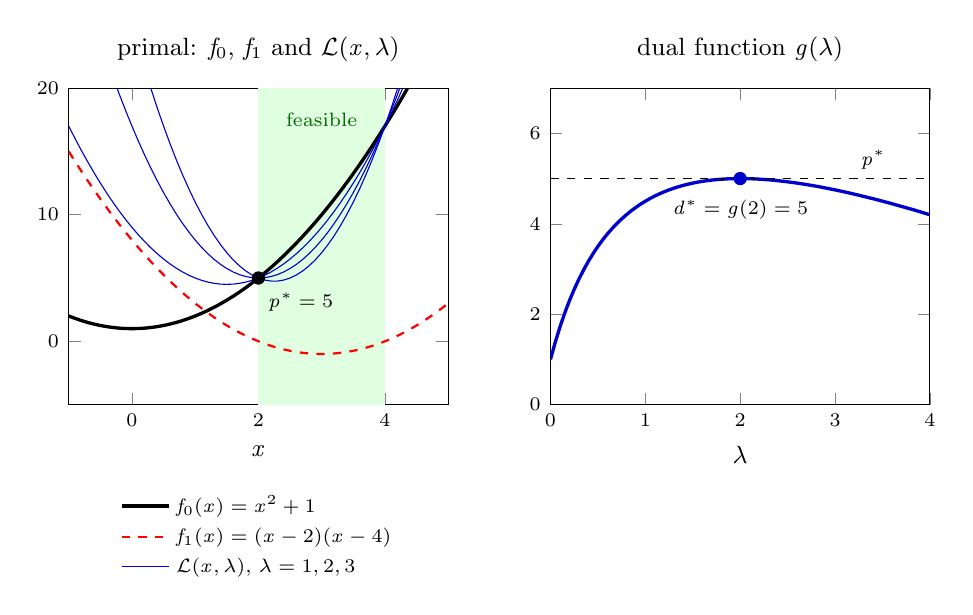
\begin{tikzpicture}
      \begin{groupplot}[group style={group size=2 by 1, horizontal sep=1.3cm}, width=6.4cm, height=5.6cm,
          tick label style={font=\scriptsize}, label style={font=\small}, title style={font=\small}]
        \nextgroupplot[title={primal: $f_0$, $f_1$ and $\mathcal L(x,\lambda)$}, xmin=-1, xmax=5, ymin=-5, ymax=20, xlabel={$x$},
            legend style={font=\scriptsize, at={(0.5,-0.25)}, anchor=north, draw=none}, legend cell align=left]
          \fill[green!12] (axis cs:2,-5) rectangle (axis cs:4,20);
          \addplot[black, very thick, domain=-1:5, samples=61] {x^2+1};
          \addlegendentry{$f_0(x)=x^2+1$}
          \addplot[red, thick, dashed, domain=-1:5, samples=61] {(x-2)*(x-4)};
          \addlegendentry{$f_1(x)=(x-2)(x-4)$}
          \addplot[blue!80!black, thin, domain=-1:5, samples=61] {x^2+1+1*(x-2)*(x-4)};
          \addlegendentry{$\mathcal L(x,\lambda)$, $\lambda=1,2,3$}
          \addplot[blue!80!black, thin, domain=-1:5, samples=61] {x^2+1+2*(x-2)*(x-4)};
          \addplot[blue!80!black, thin, domain=-1:5, samples=61] {x^2+1+3*(x-2)*(x-4)};
          \addplot[only marks, mark=*, mark size=2.2pt] coordinates {(2,5)};
          \node[font=\scriptsize, anchor=north west] at (axis cs:2,4.6) {$p^*=5$};
          \node[font=\scriptsize, green!40!black] at (axis cs:3,17.5) {feasible};
        \nextgroupplot[title={dual function $g(\lambda)$}, xmin=0, xmax=4, ymin=0, ymax=7, xlabel={$\lambda$}]
          \addplot[blue!80!black, very thick, domain=0:4, samples=81] {1+8*x-9*x^2/(1+x)};
          \addplot[black, dashed] coordinates {(0,5) (4,5)} node[pos=0.85, above, font=\scriptsize] {$p^*$};
          \addplot[only marks, mark=*, mark size=2.2pt, blue!80!black] coordinates {(2,5)};
          \node[font=\scriptsize, anchor=north] at (axis cs:2,4.75) {$d^*=g(2)=5$};
      \end{groupplot}
    \end{tikzpicture}
    \caption{Lagrange duality for the 1-D problem $\min x^2+1$ s.t.\ $(x-2)(x-4)\le0$ (adapted from Boyd and Vandenberghe, Sec.~5.1). Left: the feasible set is $[2,4]$ (green), and the optimum is $x^*=2$ with $p^*=5$. For every $\lambda\ge0$ the Lagrangian $\mathcal L(x,\lambda)=f_0(x)+\lambda f_1(x)$ (blue) lies \emph{below} $f_0$ on the feasible set, because $f_1\le0$ there; hence its minimum over all $x$, $g(\lambda)$, is a lower bound on $p^*$. Right: $g(\lambda)=1+8\lambda-\frac{9\lambda^2}{1+\lambda}$ is concave and stays below $p^*$ for all $\lambda\ge0$. The best lower bound is $d^*=g(2)=5=p^*$: the problem is convex and satisfies Slater's condition (e.\,g.\ $x=3$ is strictly feasible), so strong duality holds and the duality gap is zero.}
    \label{fig:duality}
  \end{figure}
 
\subsubsection{The Lagrange Dual Problem}

 \textbf{Problem:} how to find the best lower bound for the primal problem. The Lagrange dual problem is given by the optimization problem:
  
  \begin{align*}
    \text{maximize} \quad & g(\vect{\lambda}, \vect{\nu}) \\
    \text{subject to} \quad & \vect{\lambda} \succeq 0
  \end{align*}
  \textbf{Optimal duality gap}

Let  ${p}^*$ be the optimal value of the primal problem and ${d}^*$ the optimal value of the Lagrange dual problem. 
    
    \begin{itemize}
      \item The difference $p^*-d^*$ is the \textbf{\emph{optimal duality gap}}.
      \item If $p^*=d^*$, the duality gap is zero. In this case we talk about \textbf{\emph{strong duality}}.
      \item \textbf{\emph{Weak duality}} $d^*\leq p^*$ always holds. If $p^*> d^*$, the duality gap is positive (strong duality fails).
     \end{itemize}
 
\subsection{Slater's condition}

\textbf{Theorem}

    Given a \textbf{\emph{convex} primal optimization problem}:
    \begin{eqnarray*}
      \mbox{minimize~}  & & \quad f_0(\vect{x}) \\
      \mbox{subject to} & & \quad f_i(\vect{x}) \leq 0, \quad i=1,2,\dots, m \\
                        & & \quad \mat{A} \vect{x} = \vect{b}
    \end{eqnarray*}
    with $f_0, f_1, \ldots, f_m$ being convex. 

    If there exists an $\vect{x} \in \text{relint}~\big\{\mathcal{D} = \cap_{i=0}^m \text{dom}(f_i) \big\}$ with
    \begin{align*}
      & f_i(\vect{x}) < 0, \quad i=1,\dots,m \\
      & \mat{A}\vect{x} = \vect{b} 
    \end{align*}
    then \textbf{strong duality} holds.
   
  \subsubsection{Refinement of Slater's Condition}

 \textbf{Theorem}

    Given a \textbf{\emph{convex} primal optimization problem}. If the first $k$ constraint functions $f_1, \ldots, f_k$ are \textbf{\emph{affine}}, and 
    if there exists an $\vect{x} \in \text{relint}~\mathcal{D}$ with
    \begin{displaymath}
      \renewcommand\arraystretch{1.4}      
      \begin{array}{l l}
        f_i(\vect{x}) \le 0, \quad i=1,\dots,k                   & \text{\footnotesize (affine constraints)}\\
        f_i(\vect{x}) <   0, \quad i=k+1, \ldots, m \qquad \quad & \text{\footnotesize (convex constraints)}\\
        \mat{A}\vect{x} = \vect{b} & \\
      \end{array}
    \end{displaymath}
    then \textbf{strong duality} holds.
  
   \textbf{Note:} the refined Slater's condition reduces to \textbf{feasibility} when the constraints are all linear equalities and inequalities, and $\text{dom}(f_0)$ is open.  
 
\subsection{KKT Optimality Conditions}

  Let $\vect x^*$ be a primal and $(\vect \lambda^*, \vect \nu^*)$ dual optimal points with zero duality gap (and differentiable $f_0,f_i,h_i$). Then $\vect x^*$ minimizes $\mathcal L(\vect x, \vect \lambda^*, \vect \nu^*)$ over $\vect x$, so its gradient with respect to $\vect x$ vanishes:
 
  \begin{displaymath}
    \nabla_{\vect x} \mathcal L(\vect x^*, \vect \lambda^*, \vect \nu^*) = 
    \nabla f_0(\vect{x}^*) + 
    \sum_{i=1}^m \lambda_i^* \nabla f_i(\vect{x}^*) + 
    \sum_{i=1}^p \nu_i^* \nabla h_i(\vect{x}^*) =  \vect{0}
  \end{displaymath}
  The following four conditions on $(\vect x^*,\vect\lambda^*,\vect\nu^*)$ are called KKT conditions: 
  \begin{enumerate}
    \item \textbf{Primal constraints:} 
      \begin{itemize}
        \item $f_i(\vect{x}^*) \leq 0, \quad i = 1, 2, \dots, m$
        \item $h_i(\vect{x}^*) =    0, \quad i = 1, 2, \dots, p$  
      \end{itemize}
    \item \textbf{Dual constraints:} $\vect \lambda^* \succeq 0$  
    \item \textbf{Complementary slackness:} $ \lambda_i^* \, f_i(\vect{x}^*)= 0, \quad i=1,\dots,m$   
    \item \textbf{Gradient of the Lagrangian $\mathcal L$ w.\,r.\,t.\ $\vect x$ is zero:}
      \begin{displaymath}
        \nabla_{\vect x} \mathcal L(\vect x^*, \vect \lambda^*, \vect \nu^*) = 
        \nabla f_0(\vect{x}^*) + 
        \sum_{i=1}^m\lambda_i^* \nabla f_i(\vect{x}^*) +        
        \sum_{i=1}^p\nu_i^* \nabla h_i(\vect{x}^*) = 
        \vect{0}
      \end{displaymath}
  \end{enumerate}
   If strong duality holds and if $\vect x^*$ and $(\vect \lambda^*, \vect \nu^*)$ are optimal points, then the KKT conditions hold.\\
  
    \textbf{Complementary slackness:}\\ { $\lambda_i^* \cdot f_i(\vect{x}^*) = 0$}\\
    Important to understand this concept of complementary slackness. 
     
   \subsection{Conclusions \scriptsize ~(Boyd 2004, Sec. 5.5.3)}

  \begin{itemize}
    \item For \textbf{\emph{any} optimization problem} with differentiable objective and constraint functions for which strong duality obtains, any pair of primal and dual optimal points must satisfy the KKT conditions.  
    \item For \textbf{any \emph{convex} optimization problem} with differentiable objective and constraint functions, any points that satisfy the KKT conditions are primal and dual optimal, and have zero duality gap.  
    \item If a \textbf{\emph{convex} optimization problem} with differentiable objective and constraint functions satisfies Slater's condition, then the KKT conditions provide necessary and sufficient conditions for optimality.
  \end{itemize}

\subsection{Lessons Learned}
 
  \begin{itemize}
    \item Formalization of the primal problem using the Lagrangian 
    \item Lagrange dual function 
    \item Duality gap 
    \item Karush-Kuhn-Tucker optimality conditions
  \end{itemize}

\subsection{Comprehensive Questions}

  \begin{itemize}
    \item What is the Lagrangian of a constrained objective function? 
    \item What is the Lagrange dual function?
    \item What is the duality gap? 
    \item What are the Karush-Kuhn-Tucker optimality conditions?
  \end{itemize}
   
\newpage
\section{Support Vector Machines II}\autocite{hastie2009,bishop2006,schoelkopf2002}

\subsection{Hard Margin Problem}
  The hard margin SVM optimization problem is formulated as:
  \begin{eqnarray*}
     \mbox{minimize}   & \frac{1}{2} {\|\vect \alpha\|^2_2}\\ 
    \mbox{subject to} & \forall i: \quad y_i\cdot (\vect \alpha^T\vect x_i + \alpha_0) -1 \geq 0
  \end{eqnarray*}

\subsection{Soft Margin Problem}

  The soft margin SVM optimization problem is formulated as:
  \begin{eqnarray*}
    \mbox{minimize}   & \frac{1}{2} {\|\vect \alpha\|^2_2} + \mu \sum_i \xi_i\\
    \mbox{subject to} & \forall i: \quad -(y_i\cdot (\vect \alpha^T\vect x_i + \alpha_0) -1+\xi_i) \leq 0~, \\
    &                    \forall i: \quad -\xi_i \leq 0
  \end{eqnarray*}

  with slack variables $\xi_i$, slack weight (meta-parameter) $\mu>0$, training samples $(\vect x_i, y_i)$, $i=1,\dots,m$, and labels $y_i\in\{-1,+1\}$.

\subsection{Lagrangian}

  The solution of the \textbf{constrained convex optimization problem} requires the Lagrangian:

  \begin{eqnarray*}
    \mathcal L(\vect \alpha, \alpha_0, \vect \xi, \vect \lambda, \vect \eta)
     & = & \frac{1}{2} {\|\vect \alpha\|^2_2} + \mu \sum_i \xi_i  -\sum_i \eta_i \xi_i\\
     &   & \quad - \sum_i \lambda_i (y_i\cdot (\vect \alpha^T\vect x_i + \alpha_0) -1+\xi_i)
  \end{eqnarray*}

  where $\lambda_i\geq 0$ are the Lagrange multipliers of the margin constraints and $\eta_i\geq 0$ the Lagrange multipliers of the constraints $\xi_i\geq 0$. \\
  {\normalfont The meta-parameter (slack weight) $\mu$ is also called $C$ in the literature.}
   \textbf{Partial derivatives  I:}
 
  \begin{displaymath}
    \frac{\partial  \mathcal L(\vect \alpha, \alpha_0, \vect \xi, \vect \lambda, \vect \eta)}{\partial \vect \alpha} ~=~ 
    \vect \alpha - \sum_i \lambda_i y_i \vect x_i ~\stackrel{!}{=}~ 
    \vect 0.
  \end{displaymath}
  Thus we have:
  \begin{displaymath}
    \vect \alpha = \sum_i \lambda_i y_i \vect x_i~.
  \end{displaymath}
  \textbf{Partial derivatives  II:}
  
  \begin{displaymath}
    \frac{\partial  \mathcal L(\vect \alpha, \alpha_0, \vect \xi, \vect \lambda, \vect \eta)}{\partial \alpha_0} ~=~
   -\sum_i \lambda_i y_i ~\stackrel{!}{=}~ 
   0
  \end{displaymath}
  \textbf{Partial derivatives  III:}
  
  \begin{displaymath}
    \frac{\partial  \mathcal L(\vect \alpha, \alpha_0, \vect \xi, \vect \lambda, \vect \eta)}{\partial \xi_i} ~=~ 
    \mu - \eta_i - \lambda_i ~\stackrel{!}{=}~ 
    0
  \end{displaymath}
  
\subsection{Lagrange Dual}
  \textbf{Hard margin case} ($\xi_i=0$): we insert the stationarity conditions 
  $\vect\alpha=\sum_i\lambda_i y_i\vect x_i$ and $\sum_i\lambda_i y_i=0$ into the Lagrangian $\mathcal L(\vect\alpha,\alpha_0,\vect\lambda)$:
  
  \begin{align*}
    \mathcal L(\vect\alpha,\alpha_0,\vect\lambda)
    &= \frac{1}{2}\,\vect \alpha^T \vect \alpha - \sum_i \lambda_i \big(y_i\cdot (\vect \alpha^T\vect x_i + \alpha_0) -1\big)\\
    &= \frac{1}{2}\,\vect \alpha^T \vect \alpha - \big(\underbrace{\sum_i \lambda_i y_i\, \vect x_i}_{=\vect\alpha}\big)^T \vect \alpha - \underbrace{\sum_i \lambda_i y_i}_{=0}\,\alpha_0 + \sum_i \lambda_i\\
    &= -\frac{1}{2} \sum_i \sum_j \lambda_i \lambda_j y_i y_j \, \vect x_i^T\vect x_j +  \sum_i \lambda_i ~=:~ \mathcal L_\text{D}(\vect\lambda)
  \end{align*}
  $\vect\alpha$ and $\alpha_0$ are eliminated: the \textbf{dual Lagrangian} $\mathcal L_\text{D}$ depends on $\vect\lambda$ only.

  \medskip
  \textbf{Soft margin: same dual objective + box constraint.} \\
  Start from the soft-margin Lagrangian and sort the terms by primal variable:
  {\small
  \begin{align*}
    \mathcal L(\vect\alpha,\alpha_0,\vect\xi,\vect\lambda,\vect\eta)
    &= \frac12\vect\alpha^T\vect\alpha + \mu\sum_i\xi_i - \sum_i\eta_i\xi_i - \sum_i\lambda_i\big(y_i(\vect\alpha^T\vect x_i+\alpha_0)-1+\xi_i\big)\\
    &= \frac12\vect\alpha^T\vect\alpha - \Big(\sum_i\lambda_i y_i\vect x_i\Big)^T\vect\alpha - \alpha_0\sum_i\lambda_i y_i\\
    &\quad + \sum_i\lambda_i + \sum_i(\mu-\eta_i-\lambda_i)\,\xi_i~.
  \end{align*}
  }
  Now insert the three stationarity conditions (Partial derivatives I--III):
  \begin{itemize}
    \item $\vect\alpha=\sum_i\lambda_i y_i\vect x_i$: the first two terms give
      \[ \tfrac12\vect\alpha^T\vect\alpha-\vect\alpha^T\vect\alpha=-\tfrac12\vect\alpha^T\vect\alpha=-\tfrac12\sum_i\sum_j\lambda_i\lambda_j y_iy_j\,\vect x_i^T\vect x_j~,\]
    \item $\sum_i\lambda_i y_i=0$: the $\alpha_0$ term vanishes,
    \item $\mu-\eta_i-\lambda_i=0$: every $\xi_i$ term vanishes.
  \end{itemize}
  What remains is exactly the hard-margin dual objective
  \[
    \mathcal L_\text{D}(\vect\lambda)=-\frac12\sum_i\sum_j\lambda_i\lambda_j y_iy_j\,\vect x_i^T\vect x_j+\sum_i\lambda_i~,
  \]
  so $\vect\alpha$, $\alpha_0$, $\vect\xi$ and $\vect\eta$ are eliminated. Only the constraints change. The multipliers of inequality constraints must be non-negative, $\lambda_i\ge0$ and $\eta_i\ge0$. With $\eta_i=\mu-\lambda_i$, the second condition becomes $\mu-\lambda_i\ge0$. Together this is the \textbf{box constraint}:
  \[
    0\le \lambda_i \le \mu,\qquad \sum_i \lambda_i y_i = 0\,.
  \]
  \textbf{Soft-margin dual problem:}
  \begin{align*}
    \text{maximize}\quad & \mathcal L_\text{D}(\vect\lambda)=-\frac12\sum_i\sum_j\lambda_i\lambda_j y_iy_j\,\vect x_i^T\vect x_j+\sum_i\lambda_i\\
    \text{subject to}\quad & 0\le\lambda_i\le\mu,\quad i=1,\dots,m,\qquad \sum_i\lambda_i y_i=0~.
  \end{align*}
  Interpretation: the slack weight $\mu$ caps the influence $\lambda_i$ of each single sample, so outliers cannot dominate the solution (in the hard-margin case $\mu\to\infty$ and the upper bound disappears).

  \textbf{Benefits of the dual representation}
  \begin{itemize}
    \item The model can be reformulated using kernels.
    \item SVMs can be applied efficiently to feature spaces whose dimensionality exceeds the number of samples.
  \end{itemize}

  From Bishop: Pattern Recognition and Machine Learning
  The solution to a quadratic programming problem in $d$ variables in general has computational complexity that is $\mathcal{O}(d^3)$.
  In going to the dual formulation we have turned the original optimization problem, which involved minimizing
  \begin{eqnarray*}
    & \mbox{minimize}   & \frac{1}{2} {\|\vect \alpha\|^2_2} \\[.3cm]
    & \mbox{subject to} & \forall i: \quad y_i\cdot (\vect \alpha^T\vect x_i + \alpha_0) -1 \geq 0
  \end{eqnarray*}
  over $d$ variables, into the dual problem, which has $m$ variables.
  For a fixed set of basis functions whose number $d$ is smaller than the number $m$ of data points, the move to the dual problem appears disadvantageous. 
  However, it allows the model to be reformulated using kernels, and so the maximum margin classifier can be applied efficiently to feature spaces whose dimensionality exceeds the number of data points, including infinite feature spaces.
  The kernel formulation also makes clear the role of the constraint that the kernel function $k(\vect{x},\vect{x}')$ be positive semidefinite: then the kernel matrix is positive semidefinite, the dual objective $\mathcal L_\text{D}$ is concave, and its maximization over the feasible set is a well-defined convex problem. (Bishop words this as ``bounded below''; for the maximized dual it is concavity / boundedness from above that matters.)

  For convex optimization problems with differentiable objective and constraint functions, the duality gap is zero, if the KKT conditions are satisfied. Especially the \textbf{complementary slackness} condition is interesting for us:
  \begin{displaymath}
    \forall i: \quad \lambda_i \, f_i(\vect{x}) = 0 
  \end{displaymath}
  \textbf{Complementary slackness for hard margin SVMs:}

  \begin{displaymath}
    \forall i: \quad \lambda_i \, (y_i\cdot (\vect \alpha^T\vect x_i + \alpha_0) - 1) = 0  
  \end{displaymath}
  \textbf{Implications:} 
  
  \begin{enumerate}
    \item If $\lambda_i>0$, then $y_i \, (\vect{\alpha}^T \vect{x}_i + \alpha_0) - 1=0$, and thus:
      \begin{displaymath}
        y_i(\vect{\alpha}^T \vect{x}_i + \alpha_0) = 1~.
      \end{displaymath}
      All $\vect x_i$ with $\lambda_i>0$ lie on one of the margin hyperplanes $f(\vect x)=\pm1$; \\
      these samples are called \textbf{\emph{support vectors}}. \\  
    \item We have seen that $  \vect \alpha = \sum_i \lambda_i y_i \vect x_i $, thus the normal vector of the decision boundary is a linear combination of support vectors.
  \end{enumerate}
  \textbf{Complementary slackness for soft margin SVMs:} for both constraint types,
  \begin{displaymath}
    \forall i: \quad \lambda_i \, \big(y_i\cdot (\vect \alpha^T\vect x_i + \alpha_0) - 1+\xi_i\big) = 0, \qquad \eta_i\,\xi_i=0~.
  \end{displaymath}
  With $\eta_i=\mu-\lambda_i$: if $0<\lambda_i<\mu$, then $\xi_i=0$ and $\vect x_i$ lies on a margin hyperplane; if $\lambda_i=\mu$, then $\xi_i\ge0$: $\vect x_i$ lies on the margin hyperplane ($\xi_i=0$), inside the margin ($0<\xi_i\le1$) or is misclassified ($\xi_i>1$); if $\lambda_i=0$, then $\xi_i=0$ and $\vect x_i$ is on the correct side of the margin. All $\vect x_i$ with $\lambda_i>0$ are support vectors.
  The three cases are illustrated in Fig.~\ref{fig:svm_losses} (right), together with the hinge loss (left).

  \begin{figure}[htbp]
    \centering
    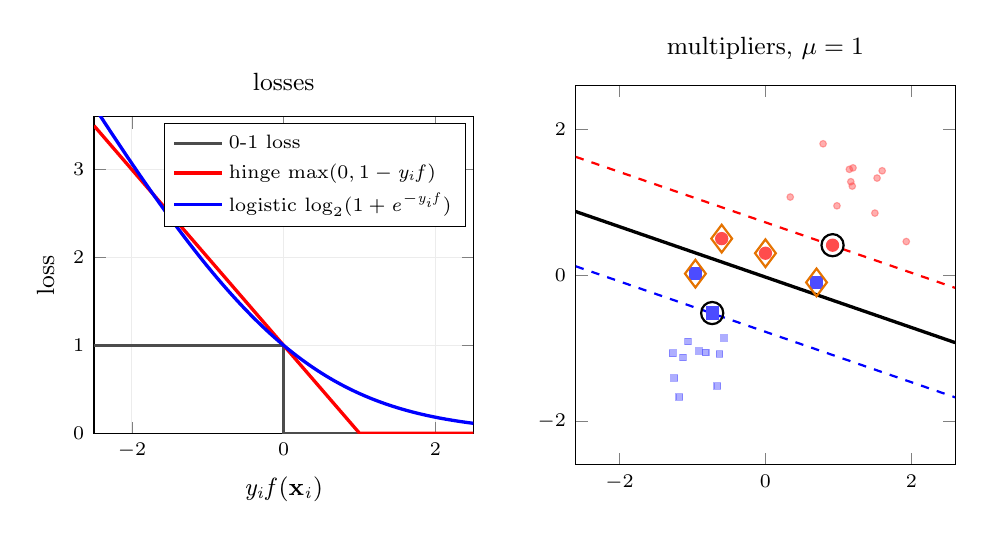
\begin{tikzpicture}
      \begin{axis}[name=loss, width=6.4cm, height=5.6cm, xmin=-2.5, xmax=2.5, ymin=0, ymax=3.6, xlabel={$y_if(\vect x_i)$}, ylabel={loss},
          title={losses}, title style={font=\small}, tick label style={font=\scriptsize}, label style={font=\small},
          legend style={font=\scriptsize, at={(0.98,0.98)}, anchor=north east}, legend cell align=left, grid=major, grid style={gray!15}]
        \addplot[gray!60!black, very thick, const plot] coordinates {(-2.5,1) (0,0) (2.5,0)};
        \addlegendentry{0-1 loss}
        \addplot[red, very thick, domain=-2.5:2.5, samples=81] {max(0,1-x)};
        \addlegendentry{hinge $\max(0,1-y_if)$}
        \addplot[blue, very thick, domain=-2.5:2.5, samples=81] {ln(1+exp(-x))/ln(2)};
        \addlegendentry{logistic $\log_2(1+e^{-y_if})$}
      \end{axis}
      \begin{axis}[at={(loss.east)}, anchor=west, xshift=1.3cm, width=6.4cm, height=6.4cm, axis equal image, xmin=-2.6, xmax=2.6, ymin=-2.6, ymax=2.6,
          xtick={-2,0,2}, ytick={-2,0,2}, tick label style={font=\scriptsize}, title={multipliers, $\mu=1$}, title style={font=\small}]
\addplot[only marks, mark=*, red!70, mark size=1.2pt, opacity=0.45, forget plot] coordinates {(1.20,1.47) (1.53,1.33) (1.93,0.46) (1.15,1.45) (1.19,1.22) (0.34,1.07) (0.79,1.80) (1.60,1.43) (1.17,1.28) (1.50,0.85) (0.98,0.95)};
\addplot[only marks, mark=square*, blue!70, mark size=1.2pt, opacity=0.45, forget plot] coordinates {(-1.27,-1.07) (-1.13,-1.13) (-0.66,-1.52) (-0.63,-1.08) (-1.25,-1.41) (-1.06,-0.91) (-0.91,-1.04) (-0.82,-1.06) (-0.57,-0.86) (-1.18,-1.67)};
\addplot[only marks, mark=*, red!70, mark size=2.2pt, forget plot] coordinates {(0.92,0.41)};
\addplot[only marks, mark=square*, blue!70, mark size=2.2pt, forget plot] coordinates {(-0.73,-0.52)};
\addplot[only marks, mark=o, mark size=4pt, thick, black, forget plot] coordinates {(0.92,0.41) (-0.73,-0.52)};
\addplot[only marks, mark=*, red!70, mark size=2.2pt, forget plot] coordinates {(0.00,0.30) (-0.60,0.50)};
\addplot[only marks, mark=square*, blue!70, mark size=2.2pt, forget plot] coordinates {(-0.96,0.02) (0.70,-0.10)};
\addplot[only marks, mark=diamond, mark size=5pt, thick, orange!90!black, forget plot] coordinates {(-0.96,0.02) (0.00,0.30) (-0.60,0.50) (0.70,-0.10)};
        \addplot[black, very thick] coordinates {(-2.600,0.871) (2.600,-0.925)};
        \addplot[red, dashed, thick] coordinates {(-2.600,1.621) (2.600,-0.175)};
        \addplot[blue, dashed, thick] coordinates {(-2.600,0.121) (2.600,-1.675)};
      \end{axis}
    \end{tikzpicture}
    \caption{Left: the hinge loss of the soft-margin SVM, $\xi_i=\max(0,1-y_if(\vect x_i))$, is a convex upper bound of the 0-1 loss. It is zero for samples beyond the margin ($y_if\ge1$) and grows linearly for margin violations; the logistic loss of logistic regression is a smooth alternative. Right: the soft-margin solution of Fig.~\ref{fig:svm_margin} with the Lagrange multipliers $\lambda_i$ from the dual problem. Faint samples: $\lambda_i=0$ (correct side of the margin, no influence on the solution). Black rings: $0<\lambda_i<\mu$ (exactly on a margin hyperplane, $\xi_i=0$). Orange diamonds: $\lambda_i=\mu$ (bounded support vectors, here margin violations with $\xi_i>0$). Only samples with $\lambda_i>0$ contribute to $\vect\alpha=\sum_i\lambda_iy_i\vect x_i$.}
    \label{fig:svm_losses}
  \end{figure}

  \textbf{Conclusion:} \\
 
  Feature vectors only appear in inner products, both in the learning and the classification phase.
  
\subsection{Feature Transforms}
 \textbf{Linear decision boundaries} in its current form have serious \textbf{limitations}:
  \begin{itemize}
    \item  Non-linearly separable data cannot be classified.
    \item  Noisy data cause problems. 
    \item  Formulation deals with vectorial data only.
  \end{itemize}
  \textbf{Possible solution:} 
  \begin{itemize}
    \item Map data into richer feature space using non-linear feature transform, \\
      then use a linear classifier.
  \end{itemize}
  We select a feature transform 
  \begin{displaymath}
    \phi: \real^d \rightarrow \real^D, \quad D \ge d
  \end{displaymath}
  such that the resulting features 
  \begin{displaymath}
    \phi(\vect x_i), \quad i = 1, 2, \dots, m
  \end{displaymath}
  are linearly separable.

    Example: Assume the decision boundary is given by the quadratic function
    \begin{displaymath}
      f(\vect x) = a_0 + a_1 x_1^2 + a_2 x_2^2 + a_3 x_1 x_2 + a_4 x_1+a_5 x_2.
    \end{displaymath}
    Obviously this is not a linear decision boundary. By the following mapping, we get features that have a linear decision boundary:
    \begin{displaymath}
      \phi(\vect x) = \left(\begin{array}{c}
                             1 \\ x_1^2 \\ x_2^2 \\ x_1x_2 \\ x_1 \\ x_2
                           \end{array}
                     \right)
    \end{displaymath}
  These feature transforms can be easily incorporated into SVMs:
  \begin{itemize}
    \item \textbf{Decision boundary:}
      {\small
        \begin{displaymath}
          f(\vect x) = \sum_i \lambda_i y_i \cdot  \langle\phi(\vect x_i), \phi(\vect x) \rangle + \alpha_0  
        \end{displaymath}
      }
      with predicted label $\hat y=\sign(f(\vect x))$ and decision boundary $\{\vect x: f(\vect x)=0\}$.
    \item The Lagrange dual problem is given by the \textbf{optimization problem}:
      {\small
        \begin{eqnarray*}
          \mbox{maximize} & -\frac{1}{2} \sum_i \sum_j \lambda_i \lambda_j y_i y_j \cdot \langle\phi(\vect x_i),\phi(\vect x_j)\rangle + \sum_i \lambda_i \\   
          \mbox{subject to}  & \vect{\lambda}\succeq 0, \quad \sum_{i} \lambda_i \, y_i = 0
        \end{eqnarray*}
      }
      (hard margin; for the soft margin add $\lambda_i\le\mu$).
  \end{itemize}
 
\subsection{Kernel Functions}

  We now define \textbf{kernel functions}:
  \begin{displaymath}
    k(\vect x, \vect x') =  \langle \phi(\vect x), \phi(\vect x') \rangle
  \end{displaymath}
  Typical kernel functions are:
  \begin{itemize}
    \item \textbf{Linear:} 
      \begin{displaymath}
        k(\vect x, \vect x') =~ \langle\vect x, \vect x'\rangle
      \end{displaymath}
    \item \textbf{Polynomial:} 
      \begin{displaymath}
        k(\vect x, \vect x') = (\langle\vect x, \vect x'\rangle + 1)^q, \quad q\in\mathbb N
      \end{displaymath}
    \item \textbf{Radial basis function:} 
      \begin{displaymath}
        k(\vect x, \vect x') = e^{-\gamma\|\vect x- \vect x'\|_2^2}
      \end{displaymath}
    \item \textbf{Sigmoid kernel:} 
      \begin{displaymath}
        k(\vect x, \vect x') =\mbox{tanh}({ \kappa \langle\vect x, \vect x'\rangle + c}), \quad \kappa>0
      \end{displaymath}
      (not positive semidefinite for all $\kappa, c$, so strictly not always a valid kernel; see Chapter \emph{Kernels})
  \end{itemize}
  
\subsection{Lessons Learned}

  \begin{itemize}
    \item Lagrangian formulation of the hard and soft margin problems    
    \item Lagrange dual representation    
    \item Idea of feature transforms
  \end{itemize}

\subsection{Comprehensive Questions}

  \begin{itemize}
    \item What is the Lagrangian of the hard margin SVM? 
    \item What are the KKT optimality conditions for the hard margin SVM? 
    \item How do we apply the KKT conditions to the Lagrange Dual? 
    \item What can we conclude from this reformulated Lagrange Dual?
  \end{itemize}
  


\newpage
% !TeX root = main.tex

\section{Kernels}\autocite{schoelkopf2002,shawetaylor2004}

\subsection{Motivation}

	Linear decision boundaries in their current form have serious limitations. First, they are often too simple to provide good decision boundaries for real-world data. Second, data that are not linearly separable cannot be classified correctly at all. Third, noisy data cause problems, because outliers can strongly shift a linear separator. Finally, the formulation deals with vectorial data only and does not directly handle other data types such as sequences.

	\textbf{Possible solution.} Map the data into a higher-dimensional feature space using a \textbf{non-linear feature transform} $\phi:\real^d\rightarrow\real^D$, $D\ge d$, and then use a linear classifier in that space, where the data may have become linearly separable. As a simple example, take two classes in $\real^2$ where one class lies inside a region around the origin and the other outside it. The transform $\phi(\vect x)=(x_1^2, x_2^2)^T$ makes them linearly separable, but only if the data are centered at the origin; for non-centered data the transform must also keep linear terms, e.\,g.\ $\phi(\vect x)=(x_1^2, x_2^2, x_1)^T$ if the data are shifted along $x_1$ (in general, both $x_1$ and $x_2$ are needed).
     
  
	\subsubsection{Dual Representation}

	\begin{itemize}
		\item The SVM \textbf{decision function} can be rewritten in dual form:
		      {\small
		      \begin{displaymath}
			      f(\vect x) =
			      \vect \alpha^T\vect x +\alpha_0 =
			      \sum_i \lambda_i y_i \, \vect x_i^T \vect x + \alpha_0
		      \end{displaymath}
		      }
		      with predicted label $\hat y = \sign(f(\vect x))$, true training labels $y_i\in\{-1,+1\}$, and Lagrange multipliers $\lambda_i\ge 0$, and where we have used the identity:
		      {\small
		      \begin{displaymath}
			      \vect \alpha = \sum_i \lambda_i y_i \, \vect x_i~.
		      \end{displaymath}
		      }
		\item The Lagrange dual problem is given by the \textbf{optimization problem}:
		      {\small
		      \begin{eqnarray*}
			      \mbox{maximize}   & & -\frac{1}{2} \sum_i \sum_j \lambda_i \lambda_j y_i y_j \cdot \vect x_i^T\vect x_j + \sum_i \lambda_i \\
			      \mbox{subject to} & & \vect{\lambda}\succeq 0, \quad \sum_{i} \lambda_i \, y_i = 0  
		      \end{eqnarray*}
		      }
	\end{itemize}

	\textbf {Conclusion:}\\
	feature vectors $\vect x_i, \vect x_j$, and $\vect x$ only appear in   \textbf{inner products}, both in the learning and the classification phase.
     
	\subsubsection{Inner Product and the Perceptron}
	The decision function that we get for the perceptron can also be written in terms of inner products:
	\begin{align*}
		f(\vect x)
		&= \left (\sum_{i\in \cal E} y_i\cdot \vect x_i \right)^T \vect x + \sum_{i\in \cal E} y_i \\
		&= \sum_{i\in \cal E} y_i\cdot \langle \vect x_i, \vect x\rangle + \sum_{i\in \cal E} y_i
	\end{align*}
	where $\cal E$ is the list of indices of training samples that required an update during perceptron training (indices may appear more than once), and the predicted label is $\hat y = \sign(f(\vect x))$ (zero initialization, $\eta=1$).

\subsection{Feature Transforms}

  	We select a   \textbf{feature transform $\phi: \real^d \rightarrow \real^D$}, $D \ge d$, such that the resulting features $\phi(\vect x_i)$, $i=1,2,\dots, m$, are linearly separable.  
	\textbf {Example}
		Assume the decision boundary is given by the quadratic function
		\begin{displaymath}
			f(\vect x) = a_0 + a_1 {x_1}^2 + a_2 {x_2}^2 + a_3 x_1 x_2 + a_4 x_1+a_5 x_2.
		\end{displaymath}
		Obviously this is not a linear decision boundary.    

		By the following mapping, we get features that have a linear decision boundary:
		\footnotesize
		\begin{displaymath}
			\phi(\vect x) = \left(
			\begin{matrix}
				%1 \\
				{x_1}^2 \\[1mm] {x_2}^2 \\ x_1 \cdot x_2 \\ x_1 \\ x_2
			\end{matrix}
			\right)
		\end{displaymath}

	Consider distances in the transformed feature space: \\
	%
	\begin{align*}
		\| \phi(\vect x)-\phi (\vect x')\|_2^2
		&= \left\langle \big(\phi(\vect x)-\phi (\vect x')\big), \big(\phi(\vect x)-\phi (\vect x')\big)\right\rangle \\
		&= \langle \phi(\vect x), \phi(\vect x)\rangle - 2 \langle \phi(\vect x), \phi(\vect x') \rangle + \langle \phi(\vect x'), \phi(\vect x') \rangle
	\end{align*}
   

	\textbf {Conclusion:} Distances can be computed by just evaluating inner products.
 	These feature transforms can be easily incorporated into SVMs: \\
	\begin{itemize}
		\item \textbf{Decision function} and predicted label $\hat y = \sign(f(\vect x))$:
		      \begin{center}
			      \small
			      \tikz[baseline]{
				      \node[fill=bl1!100,anchor=base,rounded corners=3pt] (d1) {
					      \color{bl3}
					      $\displaystyle
						      f(\vect x) = \sum_i \lambda_i \cdot y_i \cdot  \langle\phi(\vect x_i), \phi( \vect x)\rangle + \alpha_0
					      $
				      };
			      }
		      \end{center}
		      
		\item The Lagrange dual problem is given by the   \textbf{optimization problem}:
		      {\small
		      \begin{eqnarray*}
			      \mbox{maximize}   &  -\frac{1}{2} \sum_i \sum_j \lambda_i \lambda_j y_i y_j \cdot \langle\phi(\vect x_i),\phi(\vect x_j)\rangle + \sum_i \lambda_i \\     
			      \mbox{subject to} &  \vect{\lambda}\succeq 0, \quad \sum_{i} \lambda_i \, y_i = 0
		      \end{eqnarray*}
		      }
	\end{itemize}

\subsection{Kernel Functions}

	 \textbf{Definition}
		A \textbf{\emph{kernel function}} $k: {\cal X} \times {\cal X}\rightarrow \real$ on the input space ${\cal X}$ (e.\,g.\ ${\cal X}=\real^d$) is a symmetric function that maps a pair of features to a real number. For a kernel function the following property holds:
		\begin{displaymath}
			k(\vect x, \vect x') = \langle\phi(\vect x), \phi(\vect x')\rangle
		\end{displaymath}
		for some feature mapping $\phi$.\\

	\textbf {Note:} \\

	Usually the evaluation of the kernel function is much easier than the computation of transformed features followed by the inner product.\\
   \textbf{Definition}\\

		For a given set of feature vectors $\vect x_1, \vect x_2, \dots, \vect x_m$, we define the \\
		\textbf {\emph{kernel matrix}}
		\begin{eqnarray*}
			\mat K &=& [K_{i,j}]_{i,j=1,2,\dots,m}~, \quad \mbox{where} \quad K_{i,j} = \langle\phi(\vect x_i), \phi(\vect x_j)\rangle.
		\end{eqnarray*}

	\textbf {Note:} \\
	The entries of the matrix are similarity measures for transformed feature pairs.
     
	\begin{lemma}
		The kernel matrix is positive semidefinite.
	\end{lemma}
   \textbf {Proof:} We need to show $\forall \vect c\in\real^m:~\vect c^T \mat K \vect c \geq 0$~:  

	\small
	\begin{eqnarray*}
		\vect c^T \mat K \vect c
		&=& \sum_{i,j=1}^m c_ic_j K_{i,j}
		=  \sum_{i,j=1}^m c_ic_j\ \langle\phi(\vect x_i), \phi(\vect x_j)\rangle \\  
		&=& \sum_{i,j=1}^m  \langle c_i\phi(\vect x_i), c_j\phi(\vect x_j)\rangle \\  
		&=& \left \langle \sum_{i=1}^m c_i\phi(\vect x_i), \sum_{j=1}^m c_j\phi(\vect x_j)\right\rangle
		=  \left\|\sum_{i=1}^m c_i\phi(\vect x_i)\right\|_2^2
		\geq 0
	\end{eqnarray*}
     
	\textbf {Typical kernel functions:}  

	\begin{itemize}
		\item Linear: $k(\vect x, \vect x') = \langle\vect x, \vect x'\rangle$     
		\item Polynomial: $k(\vect x, \vect x') = (\langle\vect x, \vect x'\rangle+1)^q$, \quad $q\in\mathbb{N}$
		\item Laplacian radial basis function: $k(\vect x, \vect x') = e^{-\frac{\|\vect x- \vect x'\|_1}{\sigma}}$     
		\item Gaussian radial basis function: $k(\vect x, \vect x') = e^{-\frac{\|\vect x- \vect x'\|_2^2}{\sigma^2}}$ (written $e^{-\gamma\|\vect x-\vect x'\|_2^2}$ with $\gamma=1/\sigma^2$ in Chapter \emph{Support Vector Machines II})     
		\item Sigmoid kernel: $k(\vect x, \vect x') =\mbox{tanh}({ \kappa\langle\vect x, \vect x'\rangle+c})$, $\kappa>0$. \textbf{Note:} this kernel is \emph{not} positive semidefinite for all choices of $\kappa$ and $c$, so by the lemma above it is not a valid kernel in general (its kernel matrix can have negative eigenvalues); it is still used in practice for suitable parameters.\footnote{The lecture slides write $\tanh(\alpha\langle\vect x,\vect x'\rangle+\beta)$; we use $\kappa,c$ to avoid a clash with the SVM weight vector $\vect\alpha$.}
	\end{itemize}
	\textbf {Question:} \\
	Can we compute for any kernel function $k(\vect x, \vect x')$ a feature mapping $\phi$ such that the kernel function can be written as an inner product?
  	   
    The mercers theorem is interesting , but not very important for the exam. \\
	\textbf{Mercer's Theorem}\\
	For any symmetric function $k: {\cal X}\times {\cal X}\rightarrow \real$ that is square integrable on its domain and which satisfies
		\begin{displaymath}
			\int_{{\cal X}\times {\cal X}} f(\vect x)\,f(\vect x')\,k(\vect x, \vect x')\ \mathsf{d}\vect x\, \mathsf{d} \vect x' \geq 0
		\end{displaymath}

		for all square integrable functions $f$, there exist transforms $\phi_i: {\cal X}\rightarrow \real$ and $\lambda_i\geq 0$ (eigenvalues of the integral operator of $k$, not the SVM multipliers) such that:
		\begin{displaymath}
			k(\vect x, \vect x') = \sum_i \lambda_i \,\phi_i(\vect x)\,\phi_i(\vect x')
		\end{displaymath} for all $\vect x$ and $\vect x'$.

	\textbf {The Kernel Trick} \\
	In \emph{any} algorithm that is formulated in terms of a positive semidefinite kernel $k$, we can derive an alternative algorithm by replacing the kernel function $k$ by another positive semidefinite kernel $k'$.

	\subsubsection{Kernel SVMs with Soft Margins}
		\textbf {Linear kernel $\langle\vect x, \vect x'\rangle$:}
		\begin{itemize}
			\item the complexity parameter $C$ (the slack weight, denoted $\mu$ in the SVM chapters) controls the number of support vectors and
			\item hence the width of the margin and
			\item the orientation of the decision boundary   
		\end{itemize}

	\textbf{Gaussian RBF kernel $e^{-0.1\|\vect x-\vect x'\|_2^2}$:} the decision boundary is no longer linear in $\vect x$ (examples in the slides).

\subsection{Kernel PCA}
	Principal component analysis can be extended by kernels to a \textbf{non-linear} dimensionality reduction. The key idea is to rewrite the PCA eigenvalue problem such that the feature vectors only appear in inner products, which can then be replaced by a kernel.

	\textbf {PCA revisited}  

	\begin{itemize}
		\item Let $\vect x_1, \vect x_2, \dots, \vect x_m\in \real^d$ be the feature vectors with zero mean.  
		\item Compute the   \textbf{scatter matrix} (covariance matrix):
		      \begin{displaymath}
			      \mat \Sigma =
			      \frac{1}{m}\sum_{i=1}^m \vect x_i \vect x_i^T \quad
			      \in \quad \real^{d\times d}  
		      \end{displaymath}
		\item Compute the   \textbf{eigenvectors} and   \textbf{eigenvalues}:
		      \begin{displaymath}
			      \mat \Sigma \vect v_i = \lambda_i \vect v_i  
		      \end{displaymath}
		\item   \textbf{Sort} eigenvectors with decreasing eigenvalues.  
		\item Subsequent   \textbf{projection} of features to the eigenvectors.
	\end{itemize}
  	\textbf {Facts from linear algebra:} \\ 

	The eigenvectors $\vect v_i$ with $\lambda_i\neq 0$ lie in the space spanned by the feature vectors. Hence, for eigenvalues $\lambda_i\neq 0$, each eigenvector $\vect v_i$ can be written as a linear combination of the feature vectors:
		      \begin{displaymath}
			      \vect v_i = \sum_{n=1}^m a_{i,n} \, \vect x_n.
		      \end{displaymath}
   The eigenvector/-value problem for the PCA computation can now be rewritten:

	\begin{eqnarray*}
		\mat \Sigma \vect v_i
		&=& \lambda_i \vect v_i \\  
		\left( \frac{1}{m}\sum_{j=1}^m \vect x_j \vect x_j^T\right) \cdot \sum_{n=1}^m a_{i,n} \, \vect x_n
		&=& \lambda_i \sum_{n=1}^m a_{i,n} \, \vect x_n \\ 
		\sum_{j=1}^m\sum_{n=1}^m a_{i,n} \, \vect x_j \vect x_j^T\vect x_n
		&=& m \cdot \lambda_i \sum_{n=1}^m a_{i,n} \, \vect x_n
	\end{eqnarray*}
     
	Projecting both sides onto each feature vector $\vect x_l$ (multiplying from the left by $\vect x_l^T$), the following equations have to be fulfilled for all indices $l$:
		      \begin{displaymath}
			      \sum_{j=1}^m\sum_{n=1}^m a_{i,n}\vect x_l^T \vect x_j \vect x_j^T\vect x_n =
			      m \cdot \lambda_i \sum_{n=1}^m a_{i,n} \vect x_l^T\vect x_n
		      \end{displaymath}
	\textbf{Wow} -- now all feature vectors show up in terms of inner products only, so the kernel trick can be applied, \textbf{provided that the \emph{transformed} features $\phi(\vect x)$ have zero mean} (see the centering step below). For \emph{any} kernel $k(\vect x, \vect x')$, we get the \textbf{key equation for Kernel PCA}:
		      \begin{center}
			      \tikz[baseline]{
				      \node[fill=bl1!100,anchor=base,rounded corners=3pt] (d1) {
					      \color{bl3}
					      $\displaystyle \sum_{j=1}^m\sum_{n=1}^m a_{i,n} \cdot k(\vect x_l, \vect x_j) \cdot k( \vect x_j,\vect x_n) =
						      m \cdot \lambda_i \cdot \sum_{n=1}^m a_{i,n} \cdot k(\vect x_l, \vect x_n)$
				      };
			      }
		      \end{center}
 	This can be written in \textbf{matrix notation} using the symmetric, positive semi-definite kernel matrix $\mat K\in \real^{m\times m}$ and the vector $\vect a_i = (a_{i,1}, a_{i,2}, \dots, a_{i,m})^T$:

	\begin{eqnarray*}
		\mat K^2 \vect a_i        &=& m\cdot \lambda_i \mat K \vect a_i\\
		\mat K (\mat K \vect a_i) &=& m\cdot \lambda_i ( \mat K \vect a_i)
	\end{eqnarray*}
	
  	This is equivalent to
	\begin{displaymath}
		\mat K (\mat K {\vect a}_i - m\cdot \lambda_i \vect a_i) = \vect 0
	\end{displaymath}

	For $\lambda_i\neq 0$, we may choose $\vect a_i$ in the range of $\mat K$ such that $\mat K\vect a_i = m\lambda_i\,\vect a_i$. (In general, $\vect a_i$ is only defined up to addition of a null-space component of $\mat K$.)
  	The coefficient vector $\vect a_i$ for the principal components can be computed by solving the \textbf{eigenvalue/-vector problem} for $i$: \\

	\begin{center}
		$\mat K {\vect a}_i = m \lambda_i  \, \vect a_i$
	\end{center}
  
	\textbf {Note:}\\

	\small
	Kernel PCA (and thus the classical PCA as well) can be computed by solving an eigenvector/-value problem for an $(m\times m)$-matrix, where $m$ is the \textbf{cardinality of the training feature set}, instead of a $(d\times d)$-matrix. This is attractive whenever the feature dimension is much larger than the number of samples. The principal components themselves cannot be computed easily, because only the kernel is known, but \textbf{not} $\phi(\vect x)$. However, the projection $c$ of the transformed feature vector $\phi(\vect x)$ on principal component $\vect v_i= \sum_{n=1}^m a_{i,n}  \, \phi(\vect x_n)$ is easily computed by:
		      \begin{displaymath}
			      c \quad = \quad
			      \phi( \vect x)^T \vect v_i   \quad = \quad
			      \sum_{n=1}^m a_{i,n} \, \phi(\vect x)^T\phi(\vect x_n) \quad   = \quad
			      \sum_{n=1}^m a_{i,n} \, k(\vect x, \vect x_n)
		      \end{displaymath}
	For the normalization, the eigenvector scaling is chosen such that $\|\vect v_i\|_2=1$, i.e.\ $\vect a_i^T\mat K\vect a_i = m\lambda_i\|\vect a_i\|_2^2 = 1$ (this requires $\lambda_i\neq 0$).
     
It is assumed that the transformed features have   \textbf{zero mean}:

	\begin{displaymath}
		\frac{1}{m}\sum_{k=1}^m \phi(\vect x_k) = \vect 0.  
	\end{displaymath}

	This can be enforced by the   \textbf{normalization step}:
	%%
	\begin{eqnarray*}
		\tilde\phi(\vect x_i) &=& \phi(\vect x_i) - \frac{1}{m}\sum_{k=1}^m \phi(\vect x_k)
	\end{eqnarray*}
   
	Implication for the components of the   \textbf{centered kernel matrix $\tilde {\mat K}$}:

	\small
	\begin{eqnarray*}
		\tilde{K} _{i,j}
		&=& \tilde\phi(\vect x_i) ^T  \tilde\phi(\vect x_j) \\  
		&=& \left( \phi(\vect x_i) - \frac{1}{m}\sum_{k=1}^m \phi(\vect x_k) \right)^T
		\left( \phi(\vect x_j) - \frac{1}{m}\sum_{k=1}^m \phi(\vect x_k) \right) \\  
		&=& \phi(\vect x_i)^T \phi(\vect x_j) -
		\frac{1}{m}\sum_{k=1}^m \phi(\vect x_i)^T \phi(\vect x_k) -
		\frac{1}{m}\sum_{k=1}^m \phi(\vect x_k)^T  \phi(\vect x_j) + \\
		& & \quad + \frac{1}{m^2}\sum_{k,l=1}^m \phi(\vect x_k)^T \phi(\vect x_l) \\  
		&=& K_{i,j} -
		\frac{1}{m}\sum_{k=1}^m K_{i,k} -
		\frac{1}{m}\sum_{k=1}^m K_{k,j} +
		\frac{1}{m^2}\sum_{k,l=1}^m K_{k,l}
	\end{eqnarray*}
   {Example: classical vs. kernel PCA}
		\small
		Consider $m=50$ images with $1024^2$ pixels.
		The pixels define $1024^2$-dimensional feature vectors:
		\begin{displaymath}
			\vect x_1, \vect x_2, \dots, \vect x_{50} \in \real^{2^{20}}  
		\end{displaymath}

		The kernel PCA using the linear kernel
		\begin{displaymath}
			k(\vect x_i, \vect x_j) = \vect x_i^T \vect x_j
		\end{displaymath}
		requires the eigenvalue/-vector decomposition of the $(50\times 50)$ kernel matrix. \\
		The classical PCA requires the eigenvalue/-vector decomposition of a $(2^{20} \times 2^{20})$ matrix.

\subsection{String Kernels}
	\subsubsection{Kernels for Feature Sequences}

	 \textbf{Example: string kernels}
		In many domains, such as speech recognition, we do not have single feature vectors but sequences of feature vectors, possibly of different lengths. In order to use kernel methods, we therefore need a kernel for time series. The individual feature vectors are considered in $\real^d =\cal X$, and sequences of feature vectors are elements of $\cal X^*$, the set of all finite sequences over $\cal X$. The \textbf{problem} is how to define a kernel over the sequence space $\cal X^*$.

		Such a kernel has strong \textbf{implications}: it allows PCA on feature sequences -- COOL! -- and SVMs for feature sequences -- EVEN COOLER!
		Comparison of sequences via \emph{dynamic time warping} (DTW): \\

		Given two feature sequences $X, X'\in {\cal X^*}$ (with time index $t$):
		\begin{eqnarray*}
			X   &=& \big( \vect x(1), \vect x(2), \dots, \vect x(p)\big) \, ,\\
			X'  &=& \big( \vect x'(1), \vect x'(2), \dots, \vect x'(q)\big)~.
		\end{eqnarray*}
		DTW aligns the two sequences by a warping path and accumulates the distances of the matched feature vectors (schematically):
			      \begin{displaymath}
				      D_{\text{DTW}}(X,X') = \frac{1}{p}\sum_{t=1}^{p} \| \vect x\big(v(t)\big)- \vect x'\big(w(t)\big) \|_2
			      \end{displaymath}
			      where $v, w$ define the time-warping (mapping of indices to indices). The DTW kernel can then be defined as
			      \begin{displaymath}
				      k(X,X') = e^{-D_{\text{DTW}}(X,X')}\qquad (\text{not positive semidefinite in general}).
			      \end{displaymath}
		Because the kernel depends on the sequences only through the DTW distance, it automatically accounts for the temporal alignment.

\subsection{Fisher Kernels}
	A different way to construct kernels starts from a generative model: we now design kernels building on probability density functions $p(\vect x;\vect  \theta)$. Two quantities are needed, the \textbf{Fisher score (score function)}, i.\,e.\ the gradient of the log-likelihood w.\,r.\,t.\ the parameters,
		      \begin{displaymath}
			      \vect u_{\vect\theta}(\vect x) \,=\, \frac{\partial}{\partial \vect \theta} \log p(\vect x; \vect \theta)
		      \end{displaymath}
	and the \textbf{Fisher information matrix}
		      \begin{displaymath}
			      \mathcal I(\vect\theta) \,=\, E_{\vect x} \big[\vect u_{\vect\theta}(\vect x)\, \vect u_{\vect\theta}^T(\vect x)\big].
		      \end{displaymath}

	\textbf {Note:} \\
	The Fisher information matrix is the curvature of the Kullback-Leibler divergence. The Fisher kernel can be defined in   \textbf{two different ways}:

	\begin{displaymath}
		k(\vect x, \vect x') = \vect u_{\vect\theta}^T(\vect x)\, \vect u_{\vect\theta}(\vect x')
	\end{displaymath}

	or

	\begin{displaymath}
		k(\vect x, \vect x') =  \vect u_{\vect\theta}^T(\vect x)\, \mathcal I ^{-1}(\vect\theta)\, \vect u_{\vect\theta}(\vect x')
	\end{displaymath}
	\textbf {Application:} learning from partially labeled data  

	\small
	Some classification approaches require \textbf{huge collections of data} (e.\,g.\ for text or speech recognition), but labeling these data can be \textbf{time-consuming} and \textbf{costly}. If the data can be modeled with a small number of well separated components (with each component corresponding to a distinct category), little labeled data would suffice to assign a proper label to each of them. A machine learning approach that also uses the unlabeled data can therefore achieve better classification performance than one that uses only the labeled data. Fisher kernels make this possible: the generative model $p(\vect x;\vect\theta)$ can be trained on the abundant unlabeled data, and the resulting kernel is then used in a discriminative approach (e.\,g.\ an SVM) trained on the labeled data.
  
\subsection{Lessons Learned}

	\begin{itemize}
		\item Limitations of linear decision boundaries 
		\item Non-linear feature transforms
		\item Kernel function and kernel matrix 
		\item Kernel trick 
		\item Probabilities and kernels
	\end{itemize}
  
\subsection{Comprehensive Questions}
	\begin{itemize}
		\item What are the properties of kernel functions? 
		\item What is the kernel matrix?  
		\item What is the kernel trick?  
		\item How can we use kernels for string comparison?
	\end{itemize}
 
 \newpage 
\section{Laplacian Support Vector Machines}\autocite{belkin2006,melacci2011}

Modification of SVMs for different kind of data distribution. 

\subsection{Motivation}
  \textbf{Example: two class ``clock'' data set} (Fig.~\ref{fig:lapsvm_clock}).
  The data set consists of points on an inner and an outer ring, of which only two points -- one per class -- are labeled. A conventional SVM trained on just these two labels yields a straight decision boundary that cuts through both rings arbitrarily. The many unlabeled points, however, trace out the two rings and thereby reveal the geometric structure of the data. A Laplacian SVM exploits this structure, so that the decision boundary follows the circular geometry. Incorporating the geometry of the whole data set can therefore improve the classifier considerably when labels are scarce.

  \begin{figure}[htbp]
    \centering
    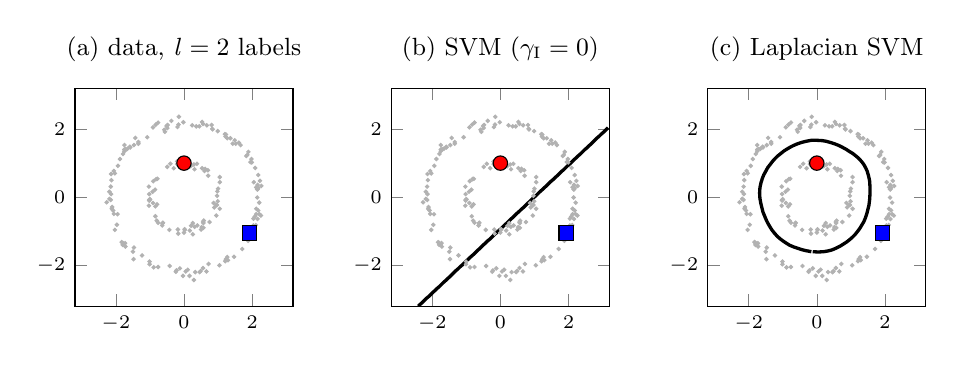
\begin{tikzpicture}
      \begin{groupplot}[group style={group size=3 by 1, horizontal sep=1.25cm, vertical sep=1.4cm}, width=4.35cm, height=4.35cm,
  axis equal image, xmin=-3.2,xmax=3.2,ymin=-3.2,ymax=3.2, xtick={-2,0,2}, ytick={-2,0,2},
  tick label style={font=\scriptsize}, title style={font=\small}]
        \nextgroupplot[title={(a) data, $l=2$ labels}]
\addplot[only marks,mark=*,mark size=0.6pt,gray!60] coordinates {(-1.02,-0.08) (1.05,-0.34) (0.60,0.77) (0.89,-0.30) (-0.40,0.98) (-0.90,0.47) (0.50,-0.95) (-0.82,0.53) (-0.84,-0.27) (0.98,0.17) (0.02,-0.96) (-1.03,-0.25) (-0.49,0.89) (0.21,-0.84) (-0.30,0.85) (-1.03,0.31) (0.70,0.79) (-0.78,0.54) (0.29,0.96) (-0.08,1.03) (0.00,-1.04) (-0.20,1.05) (-1.02,0.09) (0.99,-0.12) (0.95,-0.23) (-0.17,-1.07) (-0.79,-0.21) (-0.17,0.97) (0.53,0.85) (0.87,-0.17) (-1.02,-0.10) (0.71,0.63) (-0.76,-0.75) (0.17,-0.98) (-0.80,-0.69) (0.95,-0.54) (1.00,0.25) (-0.91,-0.17) (-0.85,0.22) (1.05,0.44) (-0.63,-0.77) (0.57,-0.76) (-0.84,-0.56) (-0.06,0.98) (0.57,-0.90) (-1.00,-0.06) (-1.00,-0.07) (0.02,-0.94) (0.62,0.83) (0.39,-0.83) (-0.43,-0.96) (0.26,-1.09) (0.31,0.82) (0.26,-0.76) (0.38,0.98) (1.05,0.59) (0.56,-0.73) (0.58,-0.69) (0.75,-0.73) (-0.92,0.16) (-0.14,0.95) (0.97,0.04) (-0.64,-0.83) (-0.18,-0.95) (0.52,-0.88) (-0.20,0.97) (0.20,0.91) (-0.62,-0.75) (0.31,-0.87) (0.97,-0.23)};
\addplot[only marks,mark=*,mark size=0.6pt,gray!60] coordinates {(1.95,1.03) (-2.19,0.16) (0.53,2.21) (1.43,1.57) (-2.15,-0.08) (0.49,-2.17) (-0.56,1.92) (0.29,-2.43) (-2.12,-0.34) (1.27,1.73) (2.21,-0.50) (-1.79,1.27) (-0.58,1.98) (1.29,-1.85) (1.61,1.60) (-0.22,-2.15) (0.83,2.01) (-1.75,1.40) (0.24,2.11) (1.21,-1.88) (-1.71,1.41) (2.12,-0.34) (-1.47,-1.48) (-0.76,-2.05) (-2.11,-0.29) (-0.83,2.13) (-1.75,1.35) (2.11,-0.82) (0.67,2.11) (2.21,-0.16) (0.11,-2.13) (-1.43,1.74) (-1.48,-1.82) (-1.59,1.48) (-1.58,1.46) (-2.19,-0.05) (2.15,0.23) (-2.14,0.09) (2.18,-0.39) (-0.48,2.12) (-0.03,-2.31) (-2.06,0.77) (0.56,2.15) (1.88,-1.28) (2.16,0.23) (-0.76,2.19) (2.15,-0.01) (-0.16,2.13) (1.27,-1.76) (-1.73,-1.35) (0.72,-1.96) (-1.50,-1.60) (-1.34,1.57) (0.16,-2.31) (2.16,0.36) (-2.03,0.70) (-1.47,1.53) (-2.15,0.31) (1.52,1.57) (0.36,2.08) (-1.97,-0.81) (-1.66,1.42) (0.56,-2.08) (-1.80,-1.40) (1.47,-1.75) (-0.24,-2.19) (-1.80,-1.34) (-0.49,2.03) (0.46,-2.20) (-0.02,2.20) (1.99,1.02) (2.26,-0.54) (-1.95,-0.50) (0.33,-2.20) (-2.08,-0.39) (-1.72,-1.45) (2.05,0.44) (0.84,1.99) (-1.01,-1.97) (-2.03,-0.96) (1.20,1.85) (2.04,-0.63) (1.22,1.78) (-2.27,-0.15) (1.36,1.73) (-0.42,-2.02) (-0.37,2.24) (1.49,1.67) (2.18,0.65) (0.99,1.94) (0.81,2.12) (-2.06,-0.49) (-2.14,0.68) (2.08,-0.57) (2.16,-0.64) (0.66,-2.18) (-1.01,-1.89) (1.23,-1.82) (2.04,-0.83) (2.27,0.33) (1.66,1.53) (-1.34,1.62) (1.86,1.24) (-1.83,-1.32) (-0.15,2.36) (-0.19,2.06) (-0.51,2.09) (1.89,1.33) (-0.12,-2.09) (-1.23,-1.71) (-1.76,-1.39) (2.23,0.48) (-1.94,0.92) (-0.89,-2.06) (1.23,1.84) (-1.75,1.53) (2.18,0.27) (1.98,1.12) (0.45,2.08) (-1.88,1.12) (-2.13,0.50) (1.71,-1.52) (-0.91,2.05) (2.12,0.29) (1.04,-2.00) (2.09,0.86) (1.83,1.21) (2.12,-0.50) (0.05,-2.18) (-1.08,1.76)};
\addplot[only marks,mark=*,mark size=2.6pt,red,draw=black] coordinates {(0.00,1.00)};
\addplot[only marks,mark=square*,mark size=2.6pt,blue,draw=black] coordinates {(1.93,-1.05)};
        \nextgroupplot[title={(b) SVM ($\gamma_\text{I}=0$)}]
\addplot[only marks,mark=*,mark size=0.6pt,gray!60] coordinates {(-1.02,-0.08) (1.05,-0.34) (0.60,0.77) (0.89,-0.30) (-0.40,0.98) (-0.90,0.47) (0.50,-0.95) (-0.82,0.53) (-0.84,-0.27) (0.98,0.17) (0.02,-0.96) (-1.03,-0.25) (-0.49,0.89) (0.21,-0.84) (-0.30,0.85) (-1.03,0.31) (0.70,0.79) (-0.78,0.54) (0.29,0.96) (-0.08,1.03) (0.00,-1.04) (-0.20,1.05) (-1.02,0.09) (0.99,-0.12) (0.95,-0.23) (-0.17,-1.07) (-0.79,-0.21) (-0.17,0.97) (0.53,0.85) (0.87,-0.17) (-1.02,-0.10) (0.71,0.63) (-0.76,-0.75) (0.17,-0.98) (-0.80,-0.69) (0.95,-0.54) (1.00,0.25) (-0.91,-0.17) (-0.85,0.22) (1.05,0.44) (-0.63,-0.77) (0.57,-0.76) (-0.84,-0.56) (-0.06,0.98) (0.57,-0.90) (-1.00,-0.06) (-1.00,-0.07) (0.02,-0.94) (0.62,0.83) (0.39,-0.83) (-0.43,-0.96) (0.26,-1.09) (0.31,0.82) (0.26,-0.76) (0.38,0.98) (1.05,0.59) (0.56,-0.73) (0.58,-0.69) (0.75,-0.73) (-0.92,0.16) (-0.14,0.95) (0.97,0.04) (-0.64,-0.83) (-0.18,-0.95) (0.52,-0.88) (-0.20,0.97) (0.20,0.91) (-0.62,-0.75) (0.31,-0.87) (0.97,-0.23)};
\addplot[only marks,mark=*,mark size=0.6pt,gray!60] coordinates {(1.95,1.03) (-2.19,0.16) (0.53,2.21) (1.43,1.57) (-2.15,-0.08) (0.49,-2.17) (-0.56,1.92) (0.29,-2.43) (-2.12,-0.34) (1.27,1.73) (2.21,-0.50) (-1.79,1.27) (-0.58,1.98) (1.29,-1.85) (1.61,1.60) (-0.22,-2.15) (0.83,2.01) (-1.75,1.40) (0.24,2.11) (1.21,-1.88) (-1.71,1.41) (2.12,-0.34) (-1.47,-1.48) (-0.76,-2.05) (-2.11,-0.29) (-0.83,2.13) (-1.75,1.35) (2.11,-0.82) (0.67,2.11) (2.21,-0.16) (0.11,-2.13) (-1.43,1.74) (-1.48,-1.82) (-1.59,1.48) (-1.58,1.46) (-2.19,-0.05) (2.15,0.23) (-2.14,0.09) (2.18,-0.39) (-0.48,2.12) (-0.03,-2.31) (-2.06,0.77) (0.56,2.15) (1.88,-1.28) (2.16,0.23) (-0.76,2.19) (2.15,-0.01) (-0.16,2.13) (1.27,-1.76) (-1.73,-1.35) (0.72,-1.96) (-1.50,-1.60) (-1.34,1.57) (0.16,-2.31) (2.16,0.36) (-2.03,0.70) (-1.47,1.53) (-2.15,0.31) (1.52,1.57) (0.36,2.08) (-1.97,-0.81) (-1.66,1.42) (0.56,-2.08) (-1.80,-1.40) (1.47,-1.75) (-0.24,-2.19) (-1.80,-1.34) (-0.49,2.03) (0.46,-2.20) (-0.02,2.20) (1.99,1.02) (2.26,-0.54) (-1.95,-0.50) (0.33,-2.20) (-2.08,-0.39) (-1.72,-1.45) (2.05,0.44) (0.84,1.99) (-1.01,-1.97) (-2.03,-0.96) (1.20,1.85) (2.04,-0.63) (1.22,1.78) (-2.27,-0.15) (1.36,1.73) (-0.42,-2.02) (-0.37,2.24) (1.49,1.67) (2.18,0.65) (0.99,1.94) (0.81,2.12) (-2.06,-0.49) (-2.14,0.68) (2.08,-0.57) (2.16,-0.64) (0.66,-2.18) (-1.01,-1.89) (1.23,-1.82) (2.04,-0.83) (2.27,0.33) (1.66,1.53) (-1.34,1.62) (1.86,1.24) (-1.83,-1.32) (-0.15,2.36) (-0.19,2.06) (-0.51,2.09) (1.89,1.33) (-0.12,-2.09) (-1.23,-1.71) (-1.76,-1.39) (2.23,0.48) (-1.94,0.92) (-0.89,-2.06) (1.23,1.84) (-1.75,1.53) (2.18,0.27) (1.98,1.12) (0.45,2.08) (-1.88,1.12) (-2.13,0.50) (1.71,-1.52) (-0.91,2.05) (2.12,0.29) (1.04,-2.00) (2.09,0.86) (1.83,1.21) (2.12,-0.50) (0.05,-2.18) (-1.08,1.76)};
\addplot[only marks,mark=*,mark size=2.6pt,red,draw=black] coordinates {(0.00,1.00)};
\addplot[only marks,mark=square*,mark size=2.6pt,blue,draw=black] coordinates {(1.93,-1.05)};
\addplot[black, very thick] coordinates {(-2.41,-3.20) (-2.36,-3.15) (-2.28,-3.08) (-2.24,-3.04) (-2.16,-2.96) (-2.11,-2.92) (-2.04,-2.85) (-1.99,-2.80) (-1.92,-2.74) (-1.86,-2.68) (-1.80,-2.63) (-1.73,-2.56) (-1.68,-2.51) (-1.60,-2.44) (-1.56,-2.40) (-1.48,-2.33) (-1.43,-2.28) (-1.36,-2.21) (-1.31,-2.16) (-1.24,-2.10) (-1.18,-2.04) (-1.12,-1.99) (-1.05,-1.92) (-1.00,-1.87) (-0.92,-1.80) (-0.88,-1.76) (-0.80,-1.69) (-0.75,-1.64) (-0.68,-1.57) (-0.62,-1.52) (-0.56,-1.46) (-0.50,-1.40) (-0.44,-1.35) (-0.37,-1.28) (-0.32,-1.24) (-0.24,-1.16) (-0.20,-1.12) (-0.12,-1.05) (-0.07,-1.00) (0.00,-0.94) (0.06,-0.88) (0.12,-0.82) (0.19,-0.76) (0.24,-0.71) (0.31,-0.64) (0.36,-0.60) (0.44,-0.52) (0.48,-0.48) (0.56,-0.41) (0.61,-0.36) (0.68,-0.30) (0.74,-0.24) (0.80,-0.18) (0.87,-0.12) (0.92,-0.07) (0.99,0.00) (1.04,0.04) (1.12,0.12) (1.16,0.16) (1.24,0.23) (1.29,0.28) (1.36,0.34) (1.42,0.40) (1.48,0.46) (1.55,0.52) (1.60,0.57) (1.68,0.64) (1.72,0.68) (1.80,0.76) (1.85,0.80) (1.92,0.87) (1.97,0.92) (2.04,0.98) (2.10,1.04) (2.16,1.10) (2.23,1.16) (2.28,1.21) (2.36,1.28) (2.40,1.32) (2.48,1.40) (2.53,1.44) (2.60,1.51) (2.66,1.56) (2.72,1.62) (2.78,1.68) (2.84,1.74) (2.91,1.80) (2.96,1.85) (3.04,1.92) (3.08,1.96) (3.16,2.04)};
        \nextgroupplot[title={(c) Laplacian SVM}]
\addplot[only marks,mark=*,mark size=0.6pt,gray!60] coordinates {(-1.02,-0.08) (1.05,-0.34) (0.60,0.77) (0.89,-0.30) (-0.40,0.98) (-0.90,0.47) (0.50,-0.95) (-0.82,0.53) (-0.84,-0.27) (0.98,0.17) (0.02,-0.96) (-1.03,-0.25) (-0.49,0.89) (0.21,-0.84) (-0.30,0.85) (-1.03,0.31) (0.70,0.79) (-0.78,0.54) (0.29,0.96) (-0.08,1.03) (0.00,-1.04) (-0.20,1.05) (-1.02,0.09) (0.99,-0.12) (0.95,-0.23) (-0.17,-1.07) (-0.79,-0.21) (-0.17,0.97) (0.53,0.85) (0.87,-0.17) (-1.02,-0.10) (0.71,0.63) (-0.76,-0.75) (0.17,-0.98) (-0.80,-0.69) (0.95,-0.54) (1.00,0.25) (-0.91,-0.17) (-0.85,0.22) (1.05,0.44) (-0.63,-0.77) (0.57,-0.76) (-0.84,-0.56) (-0.06,0.98) (0.57,-0.90) (-1.00,-0.06) (-1.00,-0.07) (0.02,-0.94) (0.62,0.83) (0.39,-0.83) (-0.43,-0.96) (0.26,-1.09) (0.31,0.82) (0.26,-0.76) (0.38,0.98) (1.05,0.59) (0.56,-0.73) (0.58,-0.69) (0.75,-0.73) (-0.92,0.16) (-0.14,0.95) (0.97,0.04) (-0.64,-0.83) (-0.18,-0.95) (0.52,-0.88) (-0.20,0.97) (0.20,0.91) (-0.62,-0.75) (0.31,-0.87) (0.97,-0.23)};
\addplot[only marks,mark=*,mark size=0.6pt,gray!60] coordinates {(1.95,1.03) (-2.19,0.16) (0.53,2.21) (1.43,1.57) (-2.15,-0.08) (0.49,-2.17) (-0.56,1.92) (0.29,-2.43) (-2.12,-0.34) (1.27,1.73) (2.21,-0.50) (-1.79,1.27) (-0.58,1.98) (1.29,-1.85) (1.61,1.60) (-0.22,-2.15) (0.83,2.01) (-1.75,1.40) (0.24,2.11) (1.21,-1.88) (-1.71,1.41) (2.12,-0.34) (-1.47,-1.48) (-0.76,-2.05) (-2.11,-0.29) (-0.83,2.13) (-1.75,1.35) (2.11,-0.82) (0.67,2.11) (2.21,-0.16) (0.11,-2.13) (-1.43,1.74) (-1.48,-1.82) (-1.59,1.48) (-1.58,1.46) (-2.19,-0.05) (2.15,0.23) (-2.14,0.09) (2.18,-0.39) (-0.48,2.12) (-0.03,-2.31) (-2.06,0.77) (0.56,2.15) (1.88,-1.28) (2.16,0.23) (-0.76,2.19) (2.15,-0.01) (-0.16,2.13) (1.27,-1.76) (-1.73,-1.35) (0.72,-1.96) (-1.50,-1.60) (-1.34,1.57) (0.16,-2.31) (2.16,0.36) (-2.03,0.70) (-1.47,1.53) (-2.15,0.31) (1.52,1.57) (0.36,2.08) (-1.97,-0.81) (-1.66,1.42) (0.56,-2.08) (-1.80,-1.40) (1.47,-1.75) (-0.24,-2.19) (-1.80,-1.34) (-0.49,2.03) (0.46,-2.20) (-0.02,2.20) (1.99,1.02) (2.26,-0.54) (-1.95,-0.50) (0.33,-2.20) (-2.08,-0.39) (-1.72,-1.45) (2.05,0.44) (0.84,1.99) (-1.01,-1.97) (-2.03,-0.96) (1.20,1.85) (2.04,-0.63) (1.22,1.78) (-2.27,-0.15) (1.36,1.73) (-0.42,-2.02) (-0.37,2.24) (1.49,1.67) (2.18,0.65) (0.99,1.94) (0.81,2.12) (-2.06,-0.49) (-2.14,0.68) (2.08,-0.57) (2.16,-0.64) (0.66,-2.18) (-1.01,-1.89) (1.23,-1.82) (2.04,-0.83) (2.27,0.33) (1.66,1.53) (-1.34,1.62) (1.86,1.24) (-1.83,-1.32) (-0.15,2.36) (-0.19,2.06) (-0.51,2.09) (1.89,1.33) (-0.12,-2.09) (-1.23,-1.71) (-1.76,-1.39) (2.23,0.48) (-1.94,0.92) (-0.89,-2.06) (1.23,1.84) (-1.75,1.53) (2.18,0.27) (1.98,1.12) (0.45,2.08) (-1.88,1.12) (-2.13,0.50) (1.71,-1.52) (-0.91,2.05) (2.12,0.29) (1.04,-2.00) (2.09,0.86) (1.83,1.21) (2.12,-0.50) (0.05,-2.18) (-1.08,1.76)};
\addplot[only marks,mark=*,mark size=2.6pt,red,draw=black] coordinates {(0.00,1.00)};
\addplot[only marks,mark=square*,mark size=2.6pt,blue,draw=black] coordinates {(1.93,-1.05)};
\addplot[black, very thick] coordinates {(-0.12,-1.60) (0.04,-1.61) (0.20,-1.60) (0.32,-1.58) (0.44,-1.55) (0.56,-1.50) (0.68,-1.44) (0.76,-1.39) (0.87,-1.32) (0.96,-1.25) (1.04,-1.18) (1.12,-1.10) (1.20,-1.00) (1.26,-0.92) (1.32,-0.82) (1.38,-0.72) (1.43,-0.60) (1.47,-0.48) (1.50,-0.36) (1.53,-0.24) (1.55,-0.08) (1.56,0.08) (1.56,0.20) (1.56,0.32) (1.55,0.48) (1.52,0.62) (1.48,0.76) (1.44,0.85) (1.38,0.96) (1.32,1.04) (1.24,1.13) (1.16,1.20) (1.06,1.28) (0.96,1.34) (0.87,1.40) (0.76,1.46) (0.64,1.52) (0.54,1.56) (0.42,1.60) (0.28,1.64) (0.16,1.66) (0.00,1.67) (-0.16,1.67) (-0.32,1.64) (-0.44,1.61) (-0.56,1.57) (-0.68,1.52) (-0.76,1.48) (-0.88,1.41) (-0.96,1.36) (-1.06,1.28) (-1.16,1.20) (-1.24,1.12) (-1.31,1.04) (-1.37,0.96) (-1.44,0.87) (-1.50,0.76) (-1.56,0.65) (-1.60,0.55) (-1.64,0.42) (-1.67,0.28) (-1.68,0.12) (-1.67,-0.04) (-1.64,-0.20) (-1.61,-0.32) (-1.58,-0.44) (-1.53,-0.56) (-1.48,-0.68) (-1.44,-0.76) (-1.37,-0.88) (-1.32,-0.96) (-1.24,-1.06) (-1.16,-1.15) (-1.08,-1.22) (-1.00,-1.28) (-0.88,-1.36) (-0.80,-1.41) (-0.68,-1.46) (-0.56,-1.50) (-0.44,-1.54) (-0.32,-1.57) (-0.16,-1.60)};
      \end{groupplot}
    \end{tikzpicture}
    \caption{Two-class ``clock'' data set: $200$ points on an inner and an outer ring, of which only $l=2$ are labeled (red circle: $y=+1$, blue square: $y=-1$); the remaining $u=198$ points (gray) are unlabeled. (b) Without the intrinsic term ($\gamma_\text{I}=0$) only the two labeled points matter, and the RBF-SVM boundary (black) is the perpendicular bisector of the two labeled points, cutting through both rings (48\,\%{} of the unlabeled points correct). (c) With the intrinsic term $\gamma_\text{I}\,\vect f^T\mat L\vect f$, the boundary must not separate points that are connected in the graph, so it runs through the empty gap between the rings (100\,\%{} correct). Computed with the dual of Sec.~\ref{sec:lapsvm} (RBF kernel, $\sigma=0.7$; $6$-nearest-neighbor graph with heat-kernel weights, $t=0.05$; $\gamma_\text{A}=1/32$, $\gamma_\text{I}=1$).}
    \label{fig:lapsvm_clock}
  \end{figure}
 
\subsection{Learning from Labeled and Unlabeled Data}
    \textbf{Training data: $S = S_l \cup S_u$.}
    The training set consists of labeled data $S_l = \{(\vect{x}_i, y_i)\}_{i=1}^{l}$ with true labels $y_i\in\{-1,+1\}$ and unlabeled data $S_u = \{\vect{x}_i\}_{i=l+1}^{m}$, i.\,e.\ $u$ feature vectors without class information, with $m=l+u$.

    \textbf{Graph Laplacian $\mat{L}$ associated with $S$.} (Bold $\mat L$ is the graph Laplacian; the Lagrangian below is $\mathcal L$.)\footnote{Notation in Belkin et al.\ (2006): labeled and unlabeled points are only distinguished by their index ranges ($1,\dots,l$ and $l+1,\dots,l+u$), the expansion coefficients are $\alpha_i$ (here $\beta_i$), the Lagrange multipliers are $\beta_i$ and $\zeta_i$ (here $\lambda_i$ and $\eta_i$), the selection matrix is $\mat J$ (here $\mat J_l$), the intrinsic term is normalized as $\frac{\gamma_I}{(l+u)^2}\vect f^T\mat L\vect f$ (here the factor is absorbed into $\gamma_\text{I}$), and the hinge loss is weighted by $\frac1l$, so their box constraint is $0\le\beta_i\le\frac1l$ (here $0\le\lambda_i\le1$). The lecture slides use $\mathcal L,\mathcal U$ for the labeled and unlabeled sets (here $S_l,S_u$) and $L$ for both the Laplacian and the Lagrangian.}
    To exploit the geometry of the entire sample $S$, the training points are treated as the nodes of a graph. The adjacency matrix $\mat{W}$ holds the edge weights $w_{ij}\ge 0$ (e.\,g.\ the heat kernel $w_{ij}=\exp(-\|\vect x_i-\vect x_j\|_2^2/(4t))$): a large weight means that $\vect x_i$ and $\vect x_j$ are close, while $w_{ij}=0$ means that there is no direct connection. The diagonal matrix $\mat{D}$ contains the degree of each node, $d_{ii} = \sum_{j=1}^m w_{ij}$, i.\,e.\ the sum of all edge weights incident to node $i$. The graph Laplacian is then
    \begin{displaymath}
      \mat{L} = \mat{D} - \mat{W}.
    \end{displaymath}

    \textbf{Kernel matrix $\mat{K}$:} $k_{ij} = k(\vect{x}_i, \vect{x}_j)$\\
    \textbf{Decision function $f(\vect{x})$, predicted label $\hat y=\sign(f(\vect x))$:} $\vect{f} = [f(\vect{x}_i),~i=1,\ldots,m]^T$ collects the outputs on all training points, labeled and unlabeled.\\
    \textbf{Regularization framework for function learning:}\\
  
  \begin{center}
        $\displaystyle
          f^* = \argmin_{f \in \mathcal{H}_k} 
          \sum_{i=1}^l V(\vect{x}_i, y_i, f) + 
          \gamma_\text{A} \, \|f\|^2_\text{A} +
          \gamma_\text{I} \, \|f\|^2_\text{I}
        $\\
        {\small where $\mathcal H_k$ is the reproducing kernel Hilbert space (RKHS) of the kernel $k$ and $\mathcal M$ denotes the data manifold.}
  \end{center}
\textbf{Loss function $V(\vect{x}_i, y_i, f)$.}
  Typical choices are the squared loss \textbf{$(y_i - f(\vect{x}_i))^2$}, which gives Regularized Least Squares (RLS), and the hinge loss \textbf{$\max [0, 1-y_i f(\vect{x}_i)]$}, which gives the SVM.
 
\textbf{Regularization terms.}
  Two complementary regularizers are used. The \emph{ambient} norm $\|\cdot\|_\text{A}$ is the norm of the function $f$ in the Reproducing Kernel Hilbert Space (RKHS); it enforces a smoothness condition on the possible solutions in the ambient space $\real^d$. The \emph{intrinsic} norm $\|\cdot\|_\text{I}$ is the norm of the function $f$ on the low-dimensional manifold; it enforces smoothness along the sampled manifold $\mathcal{M}$, i.\,e.\ neighboring points on the graph (large $w_{ij}$) should receive similar function values.

  \textbf{Reproducing Kernel Hilbert Spaces (RKHS).}
  A \textbf{Hilbert space} is an \textbf{abstract vector space} with any finite or \textbf{infinite} number of dimensions that possesses the structure of an \textbf{inner product}, which allows the measurement of \textbf{angles} and \textbf{lengths}, and that is \emph{complete} (every Cauchy sequence converges). A \textbf{Reproducing Kernel Hilbert Space} is a Hilbert space of functions that can be defined by a kernel $k$: evaluating a function $f$ at a point $\vect x$ can be written as an inner product, $f(\vect x)=\langle f, k(\vect x,\cdot)\rangle_{\mathcal H_k}$ (the reproducing property). Kernels thus provide a constructive way to work in (possibly infinite-dimensional) function spaces.
    
  \subsubsection{Manifolds}
  
  A   \textbf{manifold} is a topological space that on a small enough scale resembles  the Euclidean space. it is roughly the shape of the distribution of the features. Many high-dimensional data sets are believed to lie near a low-dimensional manifold embedded in the feature space. \\
\textbf{The Swiss Roll Problem} where the data is distributed in the shape of a swiss roll, i.\,e.\ a two-dimensional sheet rolled up in three-dimensional space. Euclidean distances in $\real^3$ ignore this two-dimensional structure, whereas manifold-aware methods such as the Laplacian regularizer respect the intrinsic geometry (Fig.~\ref{fig:swissroll}). look at slides and video for more details. 

  \begin{figure}[htbp]
    \centering
    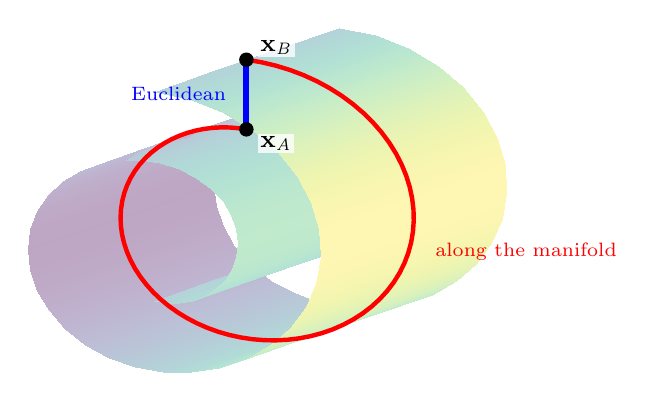
\begin{tikzpicture}
  \begin{axis}[width=9cm, height=7cm, view={25}{12}, axis lines=none, colormap/viridis,
      xmin=-15,xmax=15,ymin=0,ymax=10,zmin=-15,zmax=15, clip=false]
    \addplot3[surf, shader=interp, opacity=0.35, samples=50, samples y=4,
      domain=1.5*pi:4.5*pi, y domain=0:10, point meta=x]
      ({x*cos(deg(x))}, {y}, {x*sin(deg(x))});
    \addplot3[red, line width=1.6pt, samples=80, domain=2.5*pi:4.5*pi, variable=\t]
      ({\t*cos(deg(\t))}, {5}, {\t*sin(deg(\t))});
    \addplot3[blue, line width=2.2pt] coordinates {(0,5,{2.5*pi}) (0,5,{4.5*pi})};
\node[font=\scriptsize, blue, anchor=east] at (axis cs:-0.8,5,{3.5*pi}) {Euclidean};
\node[font=\scriptsize, red, anchor=west] at (axis cs:13.5,5,{-2}) {along the manifold};
    \addplot3[only marks, mark=*, mark size=2.4pt, black] coordinates {(0,5,{2.5*pi}) (0,5,{4.5*pi})};
    \node[font=\small, anchor=west, fill=white, inner sep=1pt, fill opacity=0.8, text opacity=1] at (axis cs:0.8,5,{2.5*pi-1.2}) {$\vect x_A$};
    \node[font=\small, anchor=west, fill=white, inner sep=1pt, fill opacity=0.8, text opacity=1] at (axis cs:0.8,5,{4.5*pi+1.2}) {$\vect x_B$};
  \end{axis}
\end{tikzpicture}
    \caption{The Swiss roll: a two-dimensional sheet rolled up in $\real^3$. The points $\vect x_A$ and $\vect x_B$ lie on neighboring layers. Their Euclidean distance (blue) is small, but their distance along the manifold (red, one full turn of the roll) is large. A nearest-neighbor graph built from densely sampled points connects only points that are close on the sheet, so the graph Laplacian measures smoothness along the manifold rather than in the ambient space.}
    \label{fig:swissroll}
  \end{figure}

\textbf{Intrinsic norm $\|\cdot\|_\text{I}$:}
  
  \begin{displaymath}
    \|f\|_\text{I}^2 = 
    \sum_{i=1}^m \sum_{j=i}^m w_{ij} \big( f(\vect{x}_i) - f(\vect{x}_j) \big)^2 = 
    \vect{f}^T \mat{L} \, \vect{f}
  \end{displaymath}
  A small example of $\mat W$, $\mat D$, $\mat L$ and of the intrinsic norm of a smooth and a non-smooth labeling is shown in Fig.~\ref{fig:lapsvm_graph}.

  \begin{figure}[htbp]
    \centering
    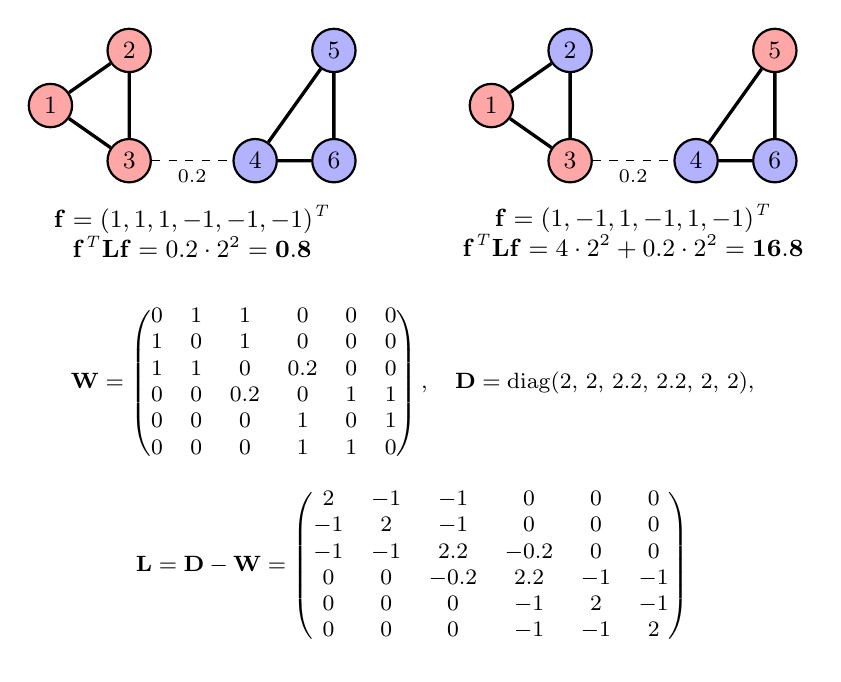
\begin{tikzpicture}[font=\small,
        nd/.style={circle,draw,thick,minimum size=5.5mm,inner sep=0pt},
        posnode/.style={nd,fill=red!35}, negnode/.style={nd,fill=blue!30}]
      % --- smooth labeling
      \begin{scope}
        \node[posnode] (a1) at (0,0) {1}; \node[posnode] (a2) at (1,0.7) {2}; \node[posnode] (a3) at (1,-0.7) {3};
        \node[negnode] (a4) at (2.6,-0.7) {4}; \node[negnode] (a5) at (3.6,0.7) {5}; \node[negnode] (a6) at (3.6,-0.7) {6};
        \draw[very thick] (a1)--(a2) (a1)--(a3) (a2)--(a3) (a4)--(a5) (a4)--(a6) (a5)--(a6);
        \draw[thin,dashed] (a3)--node[below,font=\scriptsize]{$0.2$}(a4);
        \node[align=center] at (1.8,-1.6) {$\vect f=(1,1,1,-1,-1,-1)^T$\\ $\vect f^T\mat L\vect f=0.2\cdot2^2=\mathbf{0.8}$};
      \end{scope}
      % --- rough labeling
      \begin{scope}[xshift=5.6cm]
        \node[posnode] (b1) at (0,0) {1}; \node[negnode] (b2) at (1,0.7) {2}; \node[posnode] (b3) at (1,-0.7) {3};
        \node[negnode] (b4) at (2.6,-0.7) {4}; \node[posnode] (b5) at (3.6,0.7) {5}; \node[negnode] (b6) at (3.6,-0.7) {6};
        \draw[very thick] (b1)--(b2) (b1)--(b3) (b2)--(b3) (b4)--(b5) (b4)--(b6) (b5)--(b6);
        \draw[thin,dashed] (b3)--node[below,font=\scriptsize]{$0.2$}(b4);
        \node[align=center] at (1.8,-1.6) {$\vect f=(1,-1,1,-1,1,-1)^T$\\ $\vect f^T\mat L\vect f=4\cdot 2^2+0.2\cdot2^2=\mathbf{16.8}$};
      \end{scope}
      % --- matrices
      \node[anchor=north,font=\footnotesize] (wd) at (4.6,-2.4) {$
        \mat W=\begin{pmatrix}0&1&1&0&0&0\\1&0&1&0&0&0\\1&1&0&0.2&0&0\\0&0&0.2&0&1&1\\0&0&0&1&0&1\\0&0&0&1&1&0\end{pmatrix},\quad
        \mat D=\mathrm{diag}(2,\,2,\,2.2,\,2.2,\,2,\,2),$};
      \node[anchor=north,font=\footnotesize] at ([yshift=-2pt]wd.south) {$
        \mat L=\mat D-\mat W=\begin{pmatrix}2&-1&-1&0&0&0\\-1&2&-1&0&0&0\\-1&-1&2.2&-0.2&0&0\\0&0&-0.2&2.2&-1&-1\\0&0&0&-1&2&-1\\0&0&0&-1&-1&2\end{pmatrix}$};
    \end{tikzpicture}
    \caption{Graph Laplacian and intrinsic norm for a toy graph with two clusters (edge weight $1$, thick) connected by one weak edge ($w_{34}=0.2$, dashed). Node colors show the values $f(\vect x_i)=\pm1$. Since $\vect f^T\mat L\vect f=\sum_{i<j}w_{ij}\big(f(\vect x_i)-f(\vect x_j)\big)^2$, every edge between differently colored nodes costs $w_{ij}\cdot 2^2$. Left: the labeling that is constant on each cluster only cuts the weak edge ($0.8$). Right: a labeling that alternates inside the clusters cuts four strong edges ($16.8$). Minimizing $\gamma_\text{I}\,\vect f^T\mat L\vect f$ therefore favors decision boundaries that pass through sparsely connected (low-density) regions.}
    \label{fig:lapsvm_graph}
  \end{figure}
    \textbf{Representer Theorem} (Kimeldorf and Wahba, 1970):    
  
  The solution $f^*$ of this optimization problem has the form:

  \begin{displaymath}
    f^*(\vect{x}) = \sum_{i=1}^m \beta_i^* \cdot k(\vect{x}_i, \vect{x}) + \beta_0^*
  \end{displaymath}
 
\subsection{Laplacian Support Vector Machines}\label{sec:lapsvm}
With the representer theorem, $\vect f=\mat K\vect\beta$, $\|f\|_\text{A}^2=\vect\beta^T\mat K\vect\beta$ and $\|f\|_\text{I}^2=\vect\beta^T\mat K\mat L\mat K\vect\beta$. With the hinge loss this gives the constrained \textbf{primal problem}
  \begin{eqnarray*}
    \mbox{minimize}   & & \sum_{i=1}^l \xi_i + \gamma_\text{A}\,\vect\beta^T\mat K\vect\beta + \gamma_\text{I}\,\vect\beta^T\mat K\mat L\mat K\vect\beta\\
    \mbox{subject to} & & y_i\Big(\sum_{j=1}^m \beta_j\, k(\vect x_i,\vect x_j)+\beta_0\Big)\ge 1-\xi_i,\quad \xi_i\ge 0,\quad i=1,\dots,l.
  \end{eqnarray*}
  (Compared with the soft-margin SVM, the slack weight is fixed to $1$ here; the trade-off is set by $\gamma_\text{A}$ and $\gamma_\text{I}$. Hence the box constraint below is $0\le\lambda_i\le1$ instead of $0\le\lambda_i\le\mu$.)
\textbf{Lagrange function $\mathcal L$} with multipliers $\lambda_i\ge0$ (margin constraints) and $\eta_i\ge0$ (constraints $\xi_i\ge0$):
  
  \begin{eqnarray*}
    \mathcal L(\vect\beta,\beta_0,\vect\xi,\vect\lambda,\vect\eta) 
    &=& \sum_{i=1}^l \xi_i +
        \frac{1}{2} \vect{\beta}^T (2 \gamma_\text{A} \mat{K} + 2 \gamma_\text{I} \mat{K}\mat{L}\mat{K}) \vect{\beta} -{} \\
    & & {}- \sum_{i=1}^l \lambda_i \left(y_i \Bigg(\sum_{j=1}^m \beta_j \, k(\vect{x}_i,\vect{x}_j) + \beta_0\Bigg) - 1 + \xi_i\right) -{} \\
    & & {}- \sum_{i=1}^l \eta_i \xi_i
  \end{eqnarray*}
     
    \textbf{KKT condition:} the gradient w.\,r.\,t. the primal variables $\vect{\beta}, \beta_0, \vect{\xi}$ has to vanish
   
  
  \begin{itemize}
    \item Partial derivative w.\,r.\,t. $\beta_0$:
      \begin{displaymath}
        \frac{\partial \mathcal L}{\partial \beta_0} \stackrel{!}{=} 0  \quad \Rightarrow \quad
        \sum_{i=1}^l \lambda_i y_i = 0
      \end{displaymath}
       
    \item Partial derivative w.\,r.\,t. $\xi_i$:
      \begin{displaymath}
        \frac{\partial \mathcal L}{\partial \xi_i} \stackrel{!}{=} 0  \quad \Rightarrow \quad
        1 - \lambda_i - \eta_i = 0 \quad \Rightarrow \quad
        0 \leq \lambda_i \leq 1
      \end{displaymath}
  \end{itemize}
  
    \textbf{Simplifying the Lagrangian using the two identities above:}
  
  {\small
    \begin{eqnarray*}
      \mathcal L(\vect{\beta}, \vect{\lambda}) 
      &=& \frac{1}{2} \vect{\beta}^T (2 \gamma_\text{A} \mat{K} + 2 \gamma_\text{I} \mat{K}\mat{L}\mat{K}) \vect{\beta} -{} \\
      & & {}- \sum_{i=1}^l \lambda_i \left(y_i \sum_{j=1}^m \beta_j k(\vect{x}_i,\vect{x}_j) - 1 \right) \qquad\text{(the $\beta_0$ term vanishes since $\textstyle\sum_i\lambda_iy_i=0$)} \\
      &=& \frac{1}{2} \vect{\beta}^T (2 \gamma_\text{A} \mat{K} + 2 \gamma_\text{I} \mat{K}\mat{L}\mat{K}) \vect{\beta} -
          \vect{\beta}^T \mat{K} \mat{J}_l^T \mat{Y} \vect{\lambda} +
          \sum_{i=1}^l \lambda_i
    \end{eqnarray*}
  }
  
  with $\mat{J}_l = [\mat{I}_l~\mat{0}] \in \real^{l\times m}$:
  \begin{itemize}
    \item identity matrix $\mat{I}_l \in \real^{l \times l}$
    \item rectangular matrix $\mat{0} \in \real^{l \times u}$ with all entries being 0
  \end{itemize}
  and diagonal matrix $\mat{Y} \in \real^{l \times l}$ composed by the $l$ class labels $y_i$\\
\textbf{Partial derivative w.\,r.\,t. $\vect{\beta}$:}
  
  \begin{eqnarray*}
    \frac{\partial \mathcal L}{\partial \vect{\beta}} \stackrel{!}{=} \vect{0} \\
    &\Rightarrow& 
    (2 \gamma_\text{A} \mat{K} + 2 \gamma_\text{I} \mat{K}\mat{L}\mat{K}) \vect{\beta} -
    \mat{K} \mat{J}_l^T \mat{Y} \vect{\lambda} = \vect{0}   \\
    &\Rightarrow& \text{(assuming $\mat K$ is invertible)} \\
    \vect{\beta} = (2 \gamma_\text{A} \mat{I}_m + 2 \gamma_\text{I} \mat{L}\mat{K})^{-1} 
    \mat{J}_l^T \mat{Y} \vect{\lambda}
  \end{eqnarray*}
   
    \textbf{Note:} direct relationship between parameters $\vect{\beta}$ and Lagrange multipliers $\vect{\lambda}$\\
   Substituting back in the Lagrangian expression leads to the dual problem
  \begin{displaymath}
    \max_{\vect\lambda}\ \sum_{i=1}^{l}\lambda_i - \frac{1}{2}\,\vect\lambda^T\mat Q\vect\lambda
    \quad\text{s.t.}\quad \sum_{i=1}^{l}\lambda_i y_i = 0,\ \ 0\le \lambda_i \le 1.
  \end{displaymath}
   where
  {\small
  \begin{displaymath}
    \mat{Q} = \mat{Y} \mat{J}_l \mat{K}
    (2 \gamma_\text{A} \mat{I}_m + 2 \gamma_\text{I} \mat{L}\mat{K})^{-1}
    \mat{J}_l^T \mat{Y}.
  \end{displaymath}
  }
 This is not to be memorized for the exam. 

 The decision boundaries in Figs.~\ref{fig:lapsvm_clock} and~\ref{fig:lapsvm_gammaI} were computed exactly this way: solve the dual for $\vect\lambda$, compute $\vect\beta$ from $\vect\lambda$, and obtain $\beta_0$ from a labeled point with $0<\lambda_i<1$, for which $y_if(\vect x_i)=1$. Figure~\ref{fig:lapsvm_gammaI} shows how the boundary changes with the weight $\gamma_\text{I}$ of the intrinsic term.

  \begin{figure}[htbp]
    \centering
    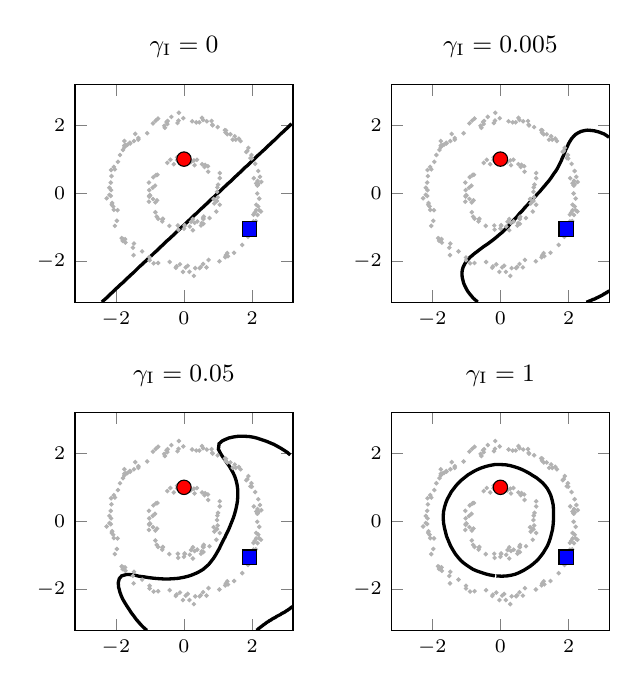
\begin{tikzpicture}
      \begin{groupplot}[group style={group size=2 by 2, horizontal sep=1.25cm, vertical sep=1.4cm}, width=4.35cm, height=4.35cm,
  axis equal image, xmin=-3.2,xmax=3.2,ymin=-3.2,ymax=3.2, xtick={-2,0,2}, ytick={-2,0,2},
  tick label style={font=\scriptsize}, title style={font=\small}]
        \nextgroupplot[title={$\gamma_\text{I}=0$}]
\addplot[only marks,mark=*,mark size=0.6pt,gray!60] coordinates {(-1.02,-0.08) (1.05,-0.34) (0.60,0.77) (0.89,-0.30) (-0.40,0.98) (-0.90,0.47) (0.50,-0.95) (-0.82,0.53) (-0.84,-0.27) (0.98,0.17) (0.02,-0.96) (-1.03,-0.25) (-0.49,0.89) (0.21,-0.84) (-0.30,0.85) (-1.03,0.31) (0.70,0.79) (-0.78,0.54) (0.29,0.96) (-0.08,1.03) (0.00,-1.04) (-0.20,1.05) (-1.02,0.09) (0.99,-0.12) (0.95,-0.23) (-0.17,-1.07) (-0.79,-0.21) (-0.17,0.97) (0.53,0.85) (0.87,-0.17) (-1.02,-0.10) (0.71,0.63) (-0.76,-0.75) (0.17,-0.98) (-0.80,-0.69) (0.95,-0.54) (1.00,0.25) (-0.91,-0.17) (-0.85,0.22) (1.05,0.44) (-0.63,-0.77) (0.57,-0.76) (-0.84,-0.56) (-0.06,0.98) (0.57,-0.90) (-1.00,-0.06) (-1.00,-0.07) (0.02,-0.94) (0.62,0.83) (0.39,-0.83) (-0.43,-0.96) (0.26,-1.09) (0.31,0.82) (0.26,-0.76) (0.38,0.98) (1.05,0.59) (0.56,-0.73) (0.58,-0.69) (0.75,-0.73) (-0.92,0.16) (-0.14,0.95) (0.97,0.04) (-0.64,-0.83) (-0.18,-0.95) (0.52,-0.88) (-0.20,0.97) (0.20,0.91) (-0.62,-0.75) (0.31,-0.87) (0.97,-0.23)};
\addplot[only marks,mark=*,mark size=0.6pt,gray!60] coordinates {(1.95,1.03) (-2.19,0.16) (0.53,2.21) (1.43,1.57) (-2.15,-0.08) (0.49,-2.17) (-0.56,1.92) (0.29,-2.43) (-2.12,-0.34) (1.27,1.73) (2.21,-0.50) (-1.79,1.27) (-0.58,1.98) (1.29,-1.85) (1.61,1.60) (-0.22,-2.15) (0.83,2.01) (-1.75,1.40) (0.24,2.11) (1.21,-1.88) (-1.71,1.41) (2.12,-0.34) (-1.47,-1.48) (-0.76,-2.05) (-2.11,-0.29) (-0.83,2.13) (-1.75,1.35) (2.11,-0.82) (0.67,2.11) (2.21,-0.16) (0.11,-2.13) (-1.43,1.74) (-1.48,-1.82) (-1.59,1.48) (-1.58,1.46) (-2.19,-0.05) (2.15,0.23) (-2.14,0.09) (2.18,-0.39) (-0.48,2.12) (-0.03,-2.31) (-2.06,0.77) (0.56,2.15) (1.88,-1.28) (2.16,0.23) (-0.76,2.19) (2.15,-0.01) (-0.16,2.13) (1.27,-1.76) (-1.73,-1.35) (0.72,-1.96) (-1.50,-1.60) (-1.34,1.57) (0.16,-2.31) (2.16,0.36) (-2.03,0.70) (-1.47,1.53) (-2.15,0.31) (1.52,1.57) (0.36,2.08) (-1.97,-0.81) (-1.66,1.42) (0.56,-2.08) (-1.80,-1.40) (1.47,-1.75) (-0.24,-2.19) (-1.80,-1.34) (-0.49,2.03) (0.46,-2.20) (-0.02,2.20) (1.99,1.02) (2.26,-0.54) (-1.95,-0.50) (0.33,-2.20) (-2.08,-0.39) (-1.72,-1.45) (2.05,0.44) (0.84,1.99) (-1.01,-1.97) (-2.03,-0.96) (1.20,1.85) (2.04,-0.63) (1.22,1.78) (-2.27,-0.15) (1.36,1.73) (-0.42,-2.02) (-0.37,2.24) (1.49,1.67) (2.18,0.65) (0.99,1.94) (0.81,2.12) (-2.06,-0.49) (-2.14,0.68) (2.08,-0.57) (2.16,-0.64) (0.66,-2.18) (-1.01,-1.89) (1.23,-1.82) (2.04,-0.83) (2.27,0.33) (1.66,1.53) (-1.34,1.62) (1.86,1.24) (-1.83,-1.32) (-0.15,2.36) (-0.19,2.06) (-0.51,2.09) (1.89,1.33) (-0.12,-2.09) (-1.23,-1.71) (-1.76,-1.39) (2.23,0.48) (-1.94,0.92) (-0.89,-2.06) (1.23,1.84) (-1.75,1.53) (2.18,0.27) (1.98,1.12) (0.45,2.08) (-1.88,1.12) (-2.13,0.50) (1.71,-1.52) (-0.91,2.05) (2.12,0.29) (1.04,-2.00) (2.09,0.86) (1.83,1.21) (2.12,-0.50) (0.05,-2.18) (-1.08,1.76)};
\addplot[only marks,mark=*,mark size=2.6pt,red,draw=black] coordinates {(0.00,1.00)};
\addplot[only marks,mark=square*,mark size=2.6pt,blue,draw=black] coordinates {(1.93,-1.05)};
\addplot[black, very thick] coordinates {(-2.41,-3.20) (-2.36,-3.15) (-2.28,-3.08) (-2.24,-3.04) (-2.16,-2.96) (-2.11,-2.92) (-2.04,-2.85) (-1.99,-2.80) (-1.92,-2.74) (-1.86,-2.68) (-1.80,-2.63) (-1.73,-2.56) (-1.68,-2.51) (-1.60,-2.44) (-1.56,-2.40) (-1.48,-2.33) (-1.43,-2.28) (-1.36,-2.21) (-1.31,-2.16) (-1.24,-2.10) (-1.18,-2.04) (-1.12,-1.99) (-1.05,-1.92) (-1.00,-1.87) (-0.92,-1.80) (-0.88,-1.76) (-0.80,-1.69) (-0.75,-1.64) (-0.68,-1.57) (-0.62,-1.52) (-0.56,-1.46) (-0.50,-1.40) (-0.44,-1.35) (-0.37,-1.28) (-0.32,-1.24) (-0.24,-1.16) (-0.20,-1.12) (-0.12,-1.05) (-0.07,-1.00) (0.00,-0.94) (0.06,-0.88) (0.12,-0.82) (0.19,-0.76) (0.24,-0.71) (0.31,-0.64) (0.36,-0.60) (0.44,-0.52) (0.48,-0.48) (0.56,-0.41) (0.61,-0.36) (0.68,-0.30) (0.74,-0.24) (0.80,-0.18) (0.87,-0.12) (0.92,-0.07) (0.99,0.00) (1.04,0.04) (1.12,0.12) (1.16,0.16) (1.24,0.23) (1.29,0.28) (1.36,0.34) (1.42,0.40) (1.48,0.46) (1.55,0.52) (1.60,0.57) (1.68,0.64) (1.72,0.68) (1.80,0.76) (1.85,0.80) (1.92,0.87) (1.97,0.92) (2.04,0.98) (2.10,1.04) (2.16,1.10) (2.23,1.16) (2.28,1.21) (2.36,1.28) (2.40,1.32) (2.48,1.40) (2.53,1.44) (2.60,1.51) (2.66,1.56) (2.72,1.62) (2.78,1.68) (2.84,1.74) (2.91,1.80) (2.96,1.85) (3.04,1.92) (3.08,1.96) (3.16,2.04)};
        \nextgroupplot[title={$\gamma_\text{I}=0.005$}]
\addplot[only marks,mark=*,mark size=0.6pt,gray!60] coordinates {(-1.02,-0.08) (1.05,-0.34) (0.60,0.77) (0.89,-0.30) (-0.40,0.98) (-0.90,0.47) (0.50,-0.95) (-0.82,0.53) (-0.84,-0.27) (0.98,0.17) (0.02,-0.96) (-1.03,-0.25) (-0.49,0.89) (0.21,-0.84) (-0.30,0.85) (-1.03,0.31) (0.70,0.79) (-0.78,0.54) (0.29,0.96) (-0.08,1.03) (0.00,-1.04) (-0.20,1.05) (-1.02,0.09) (0.99,-0.12) (0.95,-0.23) (-0.17,-1.07) (-0.79,-0.21) (-0.17,0.97) (0.53,0.85) (0.87,-0.17) (-1.02,-0.10) (0.71,0.63) (-0.76,-0.75) (0.17,-0.98) (-0.80,-0.69) (0.95,-0.54) (1.00,0.25) (-0.91,-0.17) (-0.85,0.22) (1.05,0.44) (-0.63,-0.77) (0.57,-0.76) (-0.84,-0.56) (-0.06,0.98) (0.57,-0.90) (-1.00,-0.06) (-1.00,-0.07) (0.02,-0.94) (0.62,0.83) (0.39,-0.83) (-0.43,-0.96) (0.26,-1.09) (0.31,0.82) (0.26,-0.76) (0.38,0.98) (1.05,0.59) (0.56,-0.73) (0.58,-0.69) (0.75,-0.73) (-0.92,0.16) (-0.14,0.95) (0.97,0.04) (-0.64,-0.83) (-0.18,-0.95) (0.52,-0.88) (-0.20,0.97) (0.20,0.91) (-0.62,-0.75) (0.31,-0.87) (0.97,-0.23)};
\addplot[only marks,mark=*,mark size=0.6pt,gray!60] coordinates {(1.95,1.03) (-2.19,0.16) (0.53,2.21) (1.43,1.57) (-2.15,-0.08) (0.49,-2.17) (-0.56,1.92) (0.29,-2.43) (-2.12,-0.34) (1.27,1.73) (2.21,-0.50) (-1.79,1.27) (-0.58,1.98) (1.29,-1.85) (1.61,1.60) (-0.22,-2.15) (0.83,2.01) (-1.75,1.40) (0.24,2.11) (1.21,-1.88) (-1.71,1.41) (2.12,-0.34) (-1.47,-1.48) (-0.76,-2.05) (-2.11,-0.29) (-0.83,2.13) (-1.75,1.35) (2.11,-0.82) (0.67,2.11) (2.21,-0.16) (0.11,-2.13) (-1.43,1.74) (-1.48,-1.82) (-1.59,1.48) (-1.58,1.46) (-2.19,-0.05) (2.15,0.23) (-2.14,0.09) (2.18,-0.39) (-0.48,2.12) (-0.03,-2.31) (-2.06,0.77) (0.56,2.15) (1.88,-1.28) (2.16,0.23) (-0.76,2.19) (2.15,-0.01) (-0.16,2.13) (1.27,-1.76) (-1.73,-1.35) (0.72,-1.96) (-1.50,-1.60) (-1.34,1.57) (0.16,-2.31) (2.16,0.36) (-2.03,0.70) (-1.47,1.53) (-2.15,0.31) (1.52,1.57) (0.36,2.08) (-1.97,-0.81) (-1.66,1.42) (0.56,-2.08) (-1.80,-1.40) (1.47,-1.75) (-0.24,-2.19) (-1.80,-1.34) (-0.49,2.03) (0.46,-2.20) (-0.02,2.20) (1.99,1.02) (2.26,-0.54) (-1.95,-0.50) (0.33,-2.20) (-2.08,-0.39) (-1.72,-1.45) (2.05,0.44) (0.84,1.99) (-1.01,-1.97) (-2.03,-0.96) (1.20,1.85) (2.04,-0.63) (1.22,1.78) (-2.27,-0.15) (1.36,1.73) (-0.42,-2.02) (-0.37,2.24) (1.49,1.67) (2.18,0.65) (0.99,1.94) (0.81,2.12) (-2.06,-0.49) (-2.14,0.68) (2.08,-0.57) (2.16,-0.64) (0.66,-2.18) (-1.01,-1.89) (1.23,-1.82) (2.04,-0.83) (2.27,0.33) (1.66,1.53) (-1.34,1.62) (1.86,1.24) (-1.83,-1.32) (-0.15,2.36) (-0.19,2.06) (-0.51,2.09) (1.89,1.33) (-0.12,-2.09) (-1.23,-1.71) (-1.76,-1.39) (2.23,0.48) (-1.94,0.92) (-0.89,-2.06) (1.23,1.84) (-1.75,1.53) (2.18,0.27) (1.98,1.12) (0.45,2.08) (-1.88,1.12) (-2.13,0.50) (1.71,-1.52) (-0.91,2.05) (2.12,0.29) (1.04,-2.00) (2.09,0.86) (1.83,1.21) (2.12,-0.50) (0.05,-2.18) (-1.08,1.76)};
\addplot[only marks,mark=*,mark size=2.6pt,red,draw=black] coordinates {(0.00,1.00)};
\addplot[only marks,mark=square*,mark size=2.6pt,blue,draw=black] coordinates {(1.93,-1.05)};
\addplot[black, very thick] coordinates {(-0.67,-3.20) (-0.72,-3.15) (-0.80,-3.08) (-0.84,-3.03) (-0.90,-2.96) (-0.96,-2.88) (-1.00,-2.81) (-1.04,-2.73) (-1.08,-2.64) (-1.10,-2.56) (-1.12,-2.48) (-1.13,-2.36) (-1.12,-2.26) (-1.09,-2.16) (-1.05,-2.08) (-1.00,-2.00) (-0.96,-1.96) (-0.89,-1.88) (-0.84,-1.84) (-0.76,-1.77) (-0.69,-1.72) (-0.64,-1.68) (-0.56,-1.62) (-0.48,-1.56) (-0.42,-1.52) (-0.36,-1.48) (-0.28,-1.42) (-0.20,-1.36) (-0.15,-1.32) (-0.08,-1.26) (-0.01,-1.20) (0.04,-1.16) (0.12,-1.08) (0.16,-1.04) (0.24,-0.96) (0.28,-0.91) (0.35,-0.84) (0.40,-0.78) (0.46,-0.72) (0.52,-0.65) (0.56,-0.60) (0.64,-0.52) (0.68,-0.47) (0.74,-0.40) (0.80,-0.34) (0.85,-0.28) (0.92,-0.21) (0.96,-0.16) (1.04,-0.08) (1.08,-0.03) (1.15,0.04) (1.20,0.10) (1.25,0.16) (1.32,0.24) (1.36,0.29) (1.42,0.36) (1.48,0.44) (1.52,0.50) (1.56,0.56) (1.62,0.64) (1.67,0.72) (1.71,0.80) (1.75,0.88) (1.79,0.96) (1.82,1.04) (1.86,1.12) (1.89,1.20) (1.92,1.28) (1.96,1.36) (2.00,1.45) (2.04,1.52) (2.09,1.60) (2.16,1.68) (2.20,1.72) (2.28,1.77) (2.36,1.81) (2.48,1.84) (2.56,1.85) (2.68,1.84) (2.76,1.83) (2.88,1.80) (2.96,1.77) (3.04,1.74) (3.12,1.69) (3.19,1.64)};
\addplot[black, very thick] coordinates {(3.20,-2.86) (3.18,-2.88) (3.16,-2.89) (3.12,-2.92) (3.11,-2.92) (3.08,-2.94) (3.05,-2.96) (3.04,-2.96) (3.00,-2.99) (2.98,-3.00) (2.96,-3.01) (2.92,-3.03) (2.90,-3.04) (2.88,-3.05) (2.84,-3.07) (2.81,-3.08) (2.80,-3.09) (2.76,-3.11) (2.72,-3.12) (2.72,-3.12) (2.68,-3.14) (2.64,-3.16) (2.63,-3.16) (2.60,-3.17) (2.56,-3.19) (2.52,-3.20)};
        \nextgroupplot[title={$\gamma_\text{I}=0.05$}]
\addplot[only marks,mark=*,mark size=0.6pt,gray!60] coordinates {(-1.02,-0.08) (1.05,-0.34) (0.60,0.77) (0.89,-0.30) (-0.40,0.98) (-0.90,0.47) (0.50,-0.95) (-0.82,0.53) (-0.84,-0.27) (0.98,0.17) (0.02,-0.96) (-1.03,-0.25) (-0.49,0.89) (0.21,-0.84) (-0.30,0.85) (-1.03,0.31) (0.70,0.79) (-0.78,0.54) (0.29,0.96) (-0.08,1.03) (0.00,-1.04) (-0.20,1.05) (-1.02,0.09) (0.99,-0.12) (0.95,-0.23) (-0.17,-1.07) (-0.79,-0.21) (-0.17,0.97) (0.53,0.85) (0.87,-0.17) (-1.02,-0.10) (0.71,0.63) (-0.76,-0.75) (0.17,-0.98) (-0.80,-0.69) (0.95,-0.54) (1.00,0.25) (-0.91,-0.17) (-0.85,0.22) (1.05,0.44) (-0.63,-0.77) (0.57,-0.76) (-0.84,-0.56) (-0.06,0.98) (0.57,-0.90) (-1.00,-0.06) (-1.00,-0.07) (0.02,-0.94) (0.62,0.83) (0.39,-0.83) (-0.43,-0.96) (0.26,-1.09) (0.31,0.82) (0.26,-0.76) (0.38,0.98) (1.05,0.59) (0.56,-0.73) (0.58,-0.69) (0.75,-0.73) (-0.92,0.16) (-0.14,0.95) (0.97,0.04) (-0.64,-0.83) (-0.18,-0.95) (0.52,-0.88) (-0.20,0.97) (0.20,0.91) (-0.62,-0.75) (0.31,-0.87) (0.97,-0.23)};
\addplot[only marks,mark=*,mark size=0.6pt,gray!60] coordinates {(1.95,1.03) (-2.19,0.16) (0.53,2.21) (1.43,1.57) (-2.15,-0.08) (0.49,-2.17) (-0.56,1.92) (0.29,-2.43) (-2.12,-0.34) (1.27,1.73) (2.21,-0.50) (-1.79,1.27) (-0.58,1.98) (1.29,-1.85) (1.61,1.60) (-0.22,-2.15) (0.83,2.01) (-1.75,1.40) (0.24,2.11) (1.21,-1.88) (-1.71,1.41) (2.12,-0.34) (-1.47,-1.48) (-0.76,-2.05) (-2.11,-0.29) (-0.83,2.13) (-1.75,1.35) (2.11,-0.82) (0.67,2.11) (2.21,-0.16) (0.11,-2.13) (-1.43,1.74) (-1.48,-1.82) (-1.59,1.48) (-1.58,1.46) (-2.19,-0.05) (2.15,0.23) (-2.14,0.09) (2.18,-0.39) (-0.48,2.12) (-0.03,-2.31) (-2.06,0.77) (0.56,2.15) (1.88,-1.28) (2.16,0.23) (-0.76,2.19) (2.15,-0.01) (-0.16,2.13) (1.27,-1.76) (-1.73,-1.35) (0.72,-1.96) (-1.50,-1.60) (-1.34,1.57) (0.16,-2.31) (2.16,0.36) (-2.03,0.70) (-1.47,1.53) (-2.15,0.31) (1.52,1.57) (0.36,2.08) (-1.97,-0.81) (-1.66,1.42) (0.56,-2.08) (-1.80,-1.40) (1.47,-1.75) (-0.24,-2.19) (-1.80,-1.34) (-0.49,2.03) (0.46,-2.20) (-0.02,2.20) (1.99,1.02) (2.26,-0.54) (-1.95,-0.50) (0.33,-2.20) (-2.08,-0.39) (-1.72,-1.45) (2.05,0.44) (0.84,1.99) (-1.01,-1.97) (-2.03,-0.96) (1.20,1.85) (2.04,-0.63) (1.22,1.78) (-2.27,-0.15) (1.36,1.73) (-0.42,-2.02) (-0.37,2.24) (1.49,1.67) (2.18,0.65) (0.99,1.94) (0.81,2.12) (-2.06,-0.49) (-2.14,0.68) (2.08,-0.57) (2.16,-0.64) (0.66,-2.18) (-1.01,-1.89) (1.23,-1.82) (2.04,-0.83) (2.27,0.33) (1.66,1.53) (-1.34,1.62) (1.86,1.24) (-1.83,-1.32) (-0.15,2.36) (-0.19,2.06) (-0.51,2.09) (1.89,1.33) (-0.12,-2.09) (-1.23,-1.71) (-1.76,-1.39) (2.23,0.48) (-1.94,0.92) (-0.89,-2.06) (1.23,1.84) (-1.75,1.53) (2.18,0.27) (1.98,1.12) (0.45,2.08) (-1.88,1.12) (-2.13,0.50) (1.71,-1.52) (-0.91,2.05) (2.12,0.29) (1.04,-2.00) (2.09,0.86) (1.83,1.21) (2.12,-0.50) (0.05,-2.18) (-1.08,1.76)};
\addplot[only marks,mark=*,mark size=2.6pt,red,draw=black] coordinates {(0.00,1.00)};
\addplot[only marks,mark=square*,mark size=2.6pt,blue,draw=black] coordinates {(1.93,-1.05)};
\addplot[black, very thick] coordinates {(-1.09,-3.20) (-1.18,-3.12) (-1.26,-3.04) (-1.33,-2.96) (-1.40,-2.88) (-1.48,-2.77) (-1.55,-2.68) (-1.60,-2.60) (-1.68,-2.48) (-1.73,-2.40) (-1.80,-2.28) (-1.84,-2.19) (-1.88,-2.08) (-1.92,-1.93) (-1.93,-1.80) (-1.90,-1.68) (-1.83,-1.60) (-1.69,-1.56) (-1.60,-1.56) (-1.44,-1.58) (-1.32,-1.61) (-1.16,-1.63) (-1.04,-1.65) (-0.88,-1.67) (-0.76,-1.68) (-0.60,-1.69) (-0.44,-1.69) (-0.28,-1.68) (-0.16,-1.67) (0.00,-1.64) (0.12,-1.61) (0.24,-1.57) (0.36,-1.52) (0.44,-1.48) (0.56,-1.41) (0.64,-1.34) (0.72,-1.27) (0.80,-1.17) (0.87,-1.08) (0.92,-1.00) (0.99,-0.88) (1.04,-0.79) (1.09,-0.68) (1.15,-0.56) (1.20,-0.47) (1.25,-0.36) (1.31,-0.24) (1.36,-0.12) (1.40,-0.02) (1.44,0.08) (1.48,0.20) (1.52,0.34) (1.55,0.48) (1.57,0.60) (1.58,0.76) (1.58,0.92) (1.56,1.07) (1.53,1.20) (1.49,1.32) (1.44,1.43) (1.39,1.52) (1.32,1.64) (1.26,1.72) (1.20,1.81) (1.12,1.92) (1.07,2.00) (1.01,2.12) (1.03,2.28) (1.12,2.36) (1.20,2.40) (1.32,2.45) (1.46,2.48) (1.60,2.50) (1.76,2.50) (1.92,2.49) (2.04,2.47) (2.16,2.44) (2.28,2.40) (2.40,2.36) (2.52,2.31) (2.64,2.26) (2.75,2.20) (2.84,2.15) (2.95,2.08) (3.04,2.02) (3.12,1.95)};
\addplot[black, very thick] coordinates {(3.20,-2.49) (3.17,-2.52) (3.16,-2.52) (3.12,-2.55) (3.11,-2.56) (3.08,-2.58) (3.05,-2.60) (3.04,-2.61) (3.00,-2.63) (2.99,-2.64) (2.96,-2.66) (2.92,-2.68) (2.92,-2.68) (2.88,-2.70) (2.85,-2.72) (2.84,-2.73) (2.80,-2.75) (2.78,-2.76) (2.76,-2.77) (2.72,-2.79) (2.71,-2.80) (2.68,-2.82) (2.64,-2.84) (2.64,-2.84) (2.60,-2.86) (2.57,-2.88) (2.56,-2.89) (2.52,-2.91) (2.50,-2.92) (2.48,-2.94) (2.44,-2.96) (2.44,-2.96) (2.40,-2.99) (2.39,-3.00) (2.36,-3.02) (2.33,-3.04) (2.32,-3.05) (2.28,-3.08) (2.28,-3.08) (2.24,-3.11) (2.23,-3.12) (2.20,-3.14) (2.18,-3.16) (2.16,-3.18) (2.13,-3.20)};
        \nextgroupplot[title={$\gamma_\text{I}=1$}]
\addplot[only marks,mark=*,mark size=0.6pt,gray!60] coordinates {(-1.02,-0.08) (1.05,-0.34) (0.60,0.77) (0.89,-0.30) (-0.40,0.98) (-0.90,0.47) (0.50,-0.95) (-0.82,0.53) (-0.84,-0.27) (0.98,0.17) (0.02,-0.96) (-1.03,-0.25) (-0.49,0.89) (0.21,-0.84) (-0.30,0.85) (-1.03,0.31) (0.70,0.79) (-0.78,0.54) (0.29,0.96) (-0.08,1.03) (0.00,-1.04) (-0.20,1.05) (-1.02,0.09) (0.99,-0.12) (0.95,-0.23) (-0.17,-1.07) (-0.79,-0.21) (-0.17,0.97) (0.53,0.85) (0.87,-0.17) (-1.02,-0.10) (0.71,0.63) (-0.76,-0.75) (0.17,-0.98) (-0.80,-0.69) (0.95,-0.54) (1.00,0.25) (-0.91,-0.17) (-0.85,0.22) (1.05,0.44) (-0.63,-0.77) (0.57,-0.76) (-0.84,-0.56) (-0.06,0.98) (0.57,-0.90) (-1.00,-0.06) (-1.00,-0.07) (0.02,-0.94) (0.62,0.83) (0.39,-0.83) (-0.43,-0.96) (0.26,-1.09) (0.31,0.82) (0.26,-0.76) (0.38,0.98) (1.05,0.59) (0.56,-0.73) (0.58,-0.69) (0.75,-0.73) (-0.92,0.16) (-0.14,0.95) (0.97,0.04) (-0.64,-0.83) (-0.18,-0.95) (0.52,-0.88) (-0.20,0.97) (0.20,0.91) (-0.62,-0.75) (0.31,-0.87) (0.97,-0.23)};
\addplot[only marks,mark=*,mark size=0.6pt,gray!60] coordinates {(1.95,1.03) (-2.19,0.16) (0.53,2.21) (1.43,1.57) (-2.15,-0.08) (0.49,-2.17) (-0.56,1.92) (0.29,-2.43) (-2.12,-0.34) (1.27,1.73) (2.21,-0.50) (-1.79,1.27) (-0.58,1.98) (1.29,-1.85) (1.61,1.60) (-0.22,-2.15) (0.83,2.01) (-1.75,1.40) (0.24,2.11) (1.21,-1.88) (-1.71,1.41) (2.12,-0.34) (-1.47,-1.48) (-0.76,-2.05) (-2.11,-0.29) (-0.83,2.13) (-1.75,1.35) (2.11,-0.82) (0.67,2.11) (2.21,-0.16) (0.11,-2.13) (-1.43,1.74) (-1.48,-1.82) (-1.59,1.48) (-1.58,1.46) (-2.19,-0.05) (2.15,0.23) (-2.14,0.09) (2.18,-0.39) (-0.48,2.12) (-0.03,-2.31) (-2.06,0.77) (0.56,2.15) (1.88,-1.28) (2.16,0.23) (-0.76,2.19) (2.15,-0.01) (-0.16,2.13) (1.27,-1.76) (-1.73,-1.35) (0.72,-1.96) (-1.50,-1.60) (-1.34,1.57) (0.16,-2.31) (2.16,0.36) (-2.03,0.70) (-1.47,1.53) (-2.15,0.31) (1.52,1.57) (0.36,2.08) (-1.97,-0.81) (-1.66,1.42) (0.56,-2.08) (-1.80,-1.40) (1.47,-1.75) (-0.24,-2.19) (-1.80,-1.34) (-0.49,2.03) (0.46,-2.20) (-0.02,2.20) (1.99,1.02) (2.26,-0.54) (-1.95,-0.50) (0.33,-2.20) (-2.08,-0.39) (-1.72,-1.45) (2.05,0.44) (0.84,1.99) (-1.01,-1.97) (-2.03,-0.96) (1.20,1.85) (2.04,-0.63) (1.22,1.78) (-2.27,-0.15) (1.36,1.73) (-0.42,-2.02) (-0.37,2.24) (1.49,1.67) (2.18,0.65) (0.99,1.94) (0.81,2.12) (-2.06,-0.49) (-2.14,0.68) (2.08,-0.57) (2.16,-0.64) (0.66,-2.18) (-1.01,-1.89) (1.23,-1.82) (2.04,-0.83) (2.27,0.33) (1.66,1.53) (-1.34,1.62) (1.86,1.24) (-1.83,-1.32) (-0.15,2.36) (-0.19,2.06) (-0.51,2.09) (1.89,1.33) (-0.12,-2.09) (-1.23,-1.71) (-1.76,-1.39) (2.23,0.48) (-1.94,0.92) (-0.89,-2.06) (1.23,1.84) (-1.75,1.53) (2.18,0.27) (1.98,1.12) (0.45,2.08) (-1.88,1.12) (-2.13,0.50) (1.71,-1.52) (-0.91,2.05) (2.12,0.29) (1.04,-2.00) (2.09,0.86) (1.83,1.21) (2.12,-0.50) (0.05,-2.18) (-1.08,1.76)};
\addplot[only marks,mark=*,mark size=2.6pt,red,draw=black] coordinates {(0.00,1.00)};
\addplot[only marks,mark=square*,mark size=2.6pt,blue,draw=black] coordinates {(1.93,-1.05)};
\addplot[black, very thick] coordinates {(-0.12,-1.60) (0.04,-1.61) (0.20,-1.60) (0.32,-1.58) (0.44,-1.55) (0.56,-1.50) (0.68,-1.44) (0.76,-1.39) (0.87,-1.32) (0.96,-1.25) (1.04,-1.18) (1.12,-1.10) (1.20,-1.00) (1.26,-0.92) (1.32,-0.82) (1.38,-0.72) (1.43,-0.60) (1.47,-0.48) (1.50,-0.36) (1.53,-0.24) (1.55,-0.08) (1.56,0.08) (1.56,0.20) (1.56,0.32) (1.55,0.48) (1.52,0.62) (1.48,0.76) (1.44,0.85) (1.38,0.96) (1.32,1.04) (1.24,1.13) (1.16,1.20) (1.06,1.28) (0.96,1.34) (0.87,1.40) (0.76,1.46) (0.64,1.52) (0.54,1.56) (0.42,1.60) (0.28,1.64) (0.16,1.66) (0.00,1.67) (-0.16,1.67) (-0.32,1.64) (-0.44,1.61) (-0.56,1.57) (-0.68,1.52) (-0.76,1.48) (-0.88,1.41) (-0.96,1.36) (-1.06,1.28) (-1.16,1.20) (-1.24,1.12) (-1.31,1.04) (-1.37,0.96) (-1.44,0.87) (-1.50,0.76) (-1.56,0.65) (-1.60,0.55) (-1.64,0.42) (-1.67,0.28) (-1.68,0.12) (-1.67,-0.04) (-1.64,-0.20) (-1.61,-0.32) (-1.58,-0.44) (-1.53,-0.56) (-1.48,-0.68) (-1.44,-0.76) (-1.37,-0.88) (-1.32,-0.96) (-1.24,-1.06) (-1.16,-1.15) (-1.08,-1.22) (-1.00,-1.28) (-0.88,-1.36) (-0.80,-1.41) (-0.68,-1.46) (-0.56,-1.50) (-0.44,-1.54) (-0.32,-1.57) (-0.16,-1.60)};
      \end{groupplot}
    \end{tikzpicture}
    \caption{Influence of the intrinsic regularization weight $\gamma_\text{I}$ (same data and parameters as Fig.~\ref{fig:lapsvm_clock}, $\gamma_\text{A}=1/32$ fixed). For $\gamma_\text{I}=0$ the classifier is an ordinary SVM trained on two points. With increasing $\gamma_\text{I}$, cutting through densely connected regions of the graph becomes more and more expensive, and the boundary is pushed out of the rings into the low-density gap between them.}
    \label{fig:lapsvm_gammaI}
  \end{figure}
 
\subsection{Lessons Learned}
   \textbf{Laplacian SVM:}
  
  \begin{itemize}
    \item Ongoing research topic   
    \item Extension of the Kernel SVM   
    \item Additional regularization term   
    \item Derivation of the dual problem
  \end{itemize}
 
  \newpage 
\section{The Expectation Maximization Algorithm}\autocite{dempster1977,bishop2006,hastie2009}

An important chapter for the exam. understand the steps, and if possible do the exercise to understand better. 

\subsection{Parameter Estimation}
\textbf{Goal:} Derivation of a parameter estimation technique that can deal with high-dimensional parameter spaces and with latent, hidden, or incomplete data.
  
  Two parameter estimation techniques are known from statistics. In \textbf{maximum likelihood estimation (ML estimation)}, all observations are assumed to be mutually statistically independent; the observations are kept fixed, and the (log-)likelihood function is optimized with respect to the parameters. In \textbf{maximum a-posteriori estimation (MAP estimation)}, the probability density function $p(\vect{\theta})$ of the parameters to be estimated is additionally assumed to be known, and the posterior of the parameters given the observations is maximized.
  
  Let $X$ be the observed random variable and $\p$ the parameter set. The estimates of $\p$ are denoted by $\hatp$.
  Let $x$ be a realization (observed value) of $X$.
%
  The \textbf{ML estimate} is
  \begin{displaymath}
    \hatp= \argmax_{\p}\ p(x; \p) = \argmax_{\p}\ \log p(x; \p),
  \end{displaymath}
  and the \textbf{MAP estimate} is
      {\small
        \begin{eqnarray*}
          \hatp &=& \argmax_{\p}\ p(\p|{x})\\
                &=& \argmax_{\p}\ \frac{p(\p)\,p(x|\p)}{\int p(\p')\,p(x|\p')\,\mathsf{d}\p'}\\
                &=& \argmax_{\p}\ \log p(\p) + \log p(x|\p)
        \end{eqnarray*}
      }
  Here $\p$ is considered as a random variable and its probability density function $p(\p)$ is known. The denominator (the evidence) does not depend on $\p$ and can be dropped in the maximization.
     

  \subsubsection{ML Estimation: Example}

    Let us assume a Gaussian distributed random vector:
%
    \begin{displaymath}
      p(\vect{x};\vect{\mu}, \mat{\Sigma}) = \frac{1}{\sqrt{\det(2\pi\mat{\Sigma})}}
        e^{-\frac{1}{2}(\vect{x}-\vect{\mu})^T \mat{\Sigma}^{-1} (\vect{x}-\vect{\mu})}  
    \end{displaymath}
%    
    \begin{itemize}
      \item We observe the random vectors $\vect{x}_1, \vect{x}_2, \dots, \vect{x}_m$ (training data).  
      \item Based on these training data, we have to estimate the mean vector $\vect{\mu}$ and the covariance matrix $\mat{\Sigma}$.
    \end{itemize}

    \small
    The ML estimator assumes   \textbf{mutually independent observations} and optimizes the pdf for the given set of training data:
%
    {\footnotesize
      \begin{eqnarray*}
        \{\hat{\vect{\mu}}, \hat{\mat{\Sigma}}\}
          &=& \argmax_{\vect{\mu},\mat{\Sigma}}\ \prod_{i=1}^m p(\vect{x}_i;\vect{\mu}, \mat{\Sigma}) \\   
          &=& \argmax_{\vect{\mu},\mat{\Sigma}}\ \sum_{i=1}^m \log p(\vect{x}_i;\vect{\mu}, \mat{\Sigma}) \\  
          &=& \argmax_{\vect{\mu},\mat{\Sigma}} L(\vect{x}_1, \vect{x}_2, \dots, \vect{x}_m; \vect{\mu}, \mat{\Sigma})  
      \end{eqnarray*}
    }
%
    where the   \textbf{log-likelihood function} is defined by
%
    \begin{displaymath}
        L:= L(\vect{x}_1, \vect{x}_2, \dots, \vect{x}_m; \vect{\mu}, \mat{\Sigma}) =
        \sum_{i=1}^m \log p(\vect{x}_i;\vect{\mu}, \mat{\Sigma})
      \end{displaymath}\\
    \textbf{Necessary conditions} for the estimation of the parameters are:\\
       \begin{displaymath}
         \frac{\partial L}{\partial \vect{\mu}} \stackrel{!}{=} \vect{0} 
         \quad \quad \mbox{and} \quad \quad
         \frac{\partial L}{\partial \mat{\Sigma}} \stackrel{!}{=} \mat{0}  
       \end{displaymath}\\
     Now we get for the mean vector:\\%  
       \begin{displaymath}
         \frac{\partial L}{\partial \vect{\mu}} = 
         \sum_{i=1}^m \mat{\Sigma}^{-1}(\vect x_i-\vect{\mu}) \stackrel{!}{=} 
         \vect{0}  
       \end{displaymath}\\
     and thus the   \textbf{ML estimate for the mean vector} meets our expectation:\\
      \begin{displaymath}
         \vect{\hat{\mu}} = \frac{1}{m}\sum_{i=1}^m \vect{x}_i
      \end{displaymath}\\
   \small
    Along the same lines, we get the   \textbf{estimator of the covariance matrix} by computation of the zero crossings of the partial derivatives w.\,r.\,t.\ the components of the covariance matrix:
 
    \begin{displaymath}
      \hat{\mat{\Sigma}} = \frac{1}{m} \sum_{i=1}^m (\vect x_i-\hat{\vect{\mu}})
                                                    (\vect x_i-\hat{\vect{\mu}})^T
    \end{displaymath}
  
\subsection{Gaussian Mixture Models}

recommend to implement this exercise. theory is important for the exam. So far, we have considered parameter estimation for statistical models with:  
  \begin{itemize}
    \item one class-dependent distribution component  
    \item uni- or multivariate feature vectors  
    \item the type was mostly Gaussian (normally distributed features)
  \end{itemize}
   
  Now we extend this model by representing the observations with a set of $K$ multivariate Gaussian distributions:\\
 \textbf{Problem description:} \\
  
  Given $m$ feature vectors in an $d$ dimensional space, find a set of $K$ multivariate Gaussian distributions that best represent the observations. GMMs are an example of   \textbf{\emph{unsupervised learning}} (clustering, density estimation):  

  \begin{itemize}
    \item It is not known which feature vectors are generated by which of the $K$ Gaussians  
    \item The desired output is, for each feature vector, an estimate of the probability that it is generated by distribution $k$
  \end{itemize}
     
 \textbf{GMM parameter estimation:} parameters $\vect\theta=\{\pi_k,\vect\mu_k,\mat\Sigma_k\}_{k=1}^K$
%  
  \begin{eqnarray*}
    \vect\mu_k    &\phantom{=}& \mbox{the $K$ means} \\
    \mat\Sigma_k &\phantom{=}& \mbox{the $K$ covariance matrices of size $d \times d$} \\
    \pi_k          &\phantom{=}& \mbox{mixture weights, with $\pi_k\ge 0$ and $\sum_k \pi_k=1$} \\
    z_i          &\phantom{=}& \mbox{hidden component label of $\vect x_i$, $z_i\in\{1,\dots,K\}$}\\
    \gamma_{ik}       &\phantom{=}& p(z_i=k\mid \vect x_i;\hat{\vect\theta})\ \mbox{(responsibility)}
  \end{eqnarray*}
    \textbf{Additional estimates:}
%  
  \begin{eqnarray*}
    p(\vect x;\vect\theta) &\phantom{=}& \mbox{density of observing a feature vector $\vect x$} \\
    \ell(\vect\theta)         &\phantom{=}& \mbox{overall log-likelihood function of the parameter set}
  \end{eqnarray*}
     
  \subsubsection{GMM -- Expectation}
  
  The key to the estimation problem is the \textbf{overall log-likelihood objective function $\ell(\vect\theta)$}:
  \begin{displaymath}
    \ell(\vect\theta) = \sum_{i = 1}^{m} \log p(\vect x_i;\vect\theta)
  \end{displaymath}
  
  Split $p(\vect x_i;\vect\theta)$ into its contributions from the $K$ Gaussians:
  \begin{displaymath}
    p(\vect x_i;\vect\theta) = \sum_{k=1}^{K} \pi_k \, {\mathcal N}(\vect x_i; \vect \mu_k, \mat \Sigma_k)
  \end{displaymath}

  Individual probabilities for the $K$ contributions (responsibilities):
  \begin{displaymath}
    \gamma_{ik} = p(z_i=k\mid\vect x_i;\hat{\vect\theta}) = \frac{ \hat\pi_k\,{\mathcal N}(\vect x_i; \hat{\vect \mu}_k, \hat{\mat \Sigma}_k)}{p(\vect x_i;\hat{\vect\theta})}
  \end{displaymath}
     
 \subsubsection{GMM -- Maximization}
  
    \textbf{Problem:} How do we get $\vect \mu_k, \mat \Sigma_k$ and $\pi_k$?  

  \begin{itemize}
    \item Similar to the ML estimate for the Gaussian, we maximize the log-likelihood by deriving w.\,r.\,t.\ the unknowns.     
    \item The   \textbf{ML estimates} are:
      \begin{eqnarray*}
        \hat{\vect \mu}_k 
          &=& \frac{\sum_i \gamma_{ik} \vect x_i}{\sum_i \gamma_{ik}} \\
        \hat{\mat \Sigma}_k 
          &=& \frac{\sum_i \gamma_{ik} (\vect x_i - \hat{\vect \mu}_k)(\vect x_i - \hat{\vect \mu}_k)^T}{\sum_i \gamma_{ik}} \\
        \hat{\pi}_k 
          &=& \frac{1}{m} \sum_{i=1}^m \gamma_{ik}
      \end{eqnarray*}
  \end{itemize}

  \paragraph{Where the M-step updates come from (sketch).}
  Using responsibilities $\gamma_{ik}=p(z_i=k\mid\vect x_i;\hat{\vect\theta})$ from the E-step, the stationarity conditions of the log-likelihood yield the closed-form updates.

  \textbf{Mean $\vect\mu_k$:}
  {\small
  \begin{align*}
    \frac{\partial \ell}{\partial \vect\mu_k}
      &= \sum_{i=1}^m
          \frac{\pi_k\,\mathcal N(\vect x_i;\vect\mu_k,\mat\Sigma_k)}{\sum_{l} \pi_l\,\mathcal N(\vect x_i;\vect\mu_l,\mat\Sigma_l)}\,\mat\Sigma_k^{-1}(\vect x_i-\vect\mu_k)
       = \sum_{i=1}^m \gamma_{ik}\,\mat\Sigma_k^{-1}(\vect x_i-\vect\mu_k)
       ~\stackrel{!}{=}~ \vect 0\\
    \Rightarrow\quad \hat{\vect\mu}_k &= \frac{\sum_i \gamma_{ik}\,\vect x_i}{\sum_i \gamma_{ik}}\,.
  \end{align*}
  }

  \textbf{Covariance $\mat\Sigma_k$:} same as the single-Gaussian ML estimate, but each sample is weighted by $\gamma_{ik}$:
  {\small
  \[
    \hat{\mat\Sigma}_k = \frac{\sum_i \gamma_{ik}(\vect x_i-\hat{\vect\mu}_k)(\vect x_i-\hat{\vect\mu}_k)^{T}}{\sum_i \gamma_{ik}}\,.
  \]
  }

  \textbf{Mixture weights $\pi_k$:} enforce $\sum_k \pi_k=1$ via a Lagrangian $\mathcal L = \ell(\vect\theta)+\nu(\sum_k \pi_k-1)$ and set $\partial\mathcal L/\partial \pi_k=0$ (see Sec.~\emph{Constrained Optimization} below),
  which yields $\hat \pi_k=\tfrac{1}{m}\sum_i \gamma_{ik}$.

  \subsubsection*{GMM Parameter Estimation}
    \textbf{Observations:}

  \begin{itemize}
    \item If we know the values for the parameters ($\vect \mu_k, \mat \Sigma_k, \pi_k$), we can compute the expectations (\textbf {E-step}).     
    \item Once we have the expectations we can compute improved values for the parameters (\textbf {M-step}).
  \end{itemize}
     
  We have found an   \textbf{iterative solution scheme} for the nonlinear GMM parameter estimation problem:

  \begin{itemize}
    \item \emph{Right at} the ML solution both E- and M-step relations hold.   
    \item The ML parameters are a stationary point for the E- and M-step.   
    \item Starting from any parameter values, an iteration of the E-step combined with an M-step will not decrease $\ell$.
  \end{itemize}
\textbf{EM algorithm for GMM parameter estimation:}\\
refer to slides\\

  \begin{centernss}
    \begin{struktogramm}(100,50)
      \assign{Initialization: $\vect \mu_k^{(0)}, \mat \Sigma_k^{(0)}, \pi_k^{(0)}$}
      \assign{$j \gets 0$}
      \until{$\left|\ell^{(j+1)}-\ell^{(j)}\right| < \varepsilon$}
        \assign{\textbf{Expectation step}: compute new values for $\gamma_{ik}, \ell$}
        \assign{\textbf{Maximization step}: compute $\vect \mu_k^{(j+1)}, \mat \Sigma_k^{(j+1)}, \pi_k^{(j+1)}$}
        \assign{$j \gets j+1$}
      \untilend
      \assign{Output: estimates $\hat{\vect \mu}_k, \hat{\mat \Sigma}_k, \hat{\pi}_k$}
    \end{struktogramm}
  \end{centernss}

\subsection{Missing Information Principle}

  A colloquial formulation of the   \textbf{missing information principle (MIP)} is as simple as:  observable information $=$ complete information $-$ hidden information

     
\textbf{Mathematical formalization of the MIP:}
  Let $X$ be the observable random variable, $Z$ the hidden random variable, and $\p$ the parameter set.
   
  The joint density of the events $x$ (observation) and $z$ (hidden) is:
  \begin{displaymath}
    p(x,z; \p) = p(x; \p)\, p(z \mid x; \p)
  \end{displaymath}
%
  and thus:
  \begin{displaymath}
    p(x; \p)= \frac{p(x, z; \p)}{p(z\mid x; \p)}
  \end{displaymath}
    The mathematical formulation of the MIP is:
  \begin{displaymath}
    -\log p(x; \p) = -\log p(x, z; \p) -(-\log p(z\mid x; \p))
  \end{displaymath}
  
  \textbf{Key Equation}\\
  We now consider the mathematical formulation of the key equation and derive an iterative parameter estimation scheme:

  Let $j$ denote the iteration index (note: $i$ is used as the sample index in this course), and consider the key equation for the $(j+1)$-st iteration:
     {\small
       \begin{displaymath}
         \log p\left(x    ; \hatp^{(j+1)} \right) =
         \log p\left(x, z ; \hatp^{(j+1)} \right) -
         \log p\left(z\mid x  ; \hatp^{(j+1)} \right)~.
       \end{displaymath}
     }
  Now we multiply both sides with $p\left( z\mid x ; \hatp^{(j)} \right)$, the posterior of the hidden event under the current estimate, and integrate over the hidden event $z$:
     \footnotesize
     \begin{eqnarray*}
             \int p\left(z\mid x ; \hatp^{(j)} \right) \log p\left( x ;   \hatp^{(j+1)} \right)\, \mathsf{d}z
         &=& \int p\left(z\mid x ; \hatp^{(j)} \right) \log p\left(x, z ; \hatp^{(j+1)} \right)\, \mathsf{d}z -{} \\
         & & \int p\left(z\mid x ; \hatp^{(j)} \right) \log p\left(z\mid x  ; \hatp^{(j+1)} \right)\, \mathsf{d}z
     \end{eqnarray*}
 \normalsize
 Now consider the left hand side of this equation:
  
  \begin{eqnarray*}
          & & \int p\left(z\mid x ; \hatp^{(j)}   \right) \, \log p\left( x ; \hatp^{(j+1)} \right)\ \mathsf{d}z ={} \\  
          &=& \log p\left(x   ; \hatp^{(j+1)} \right) \, \int p\left( z\mid x ; \hatp^{(j)} \right)\ \mathsf{d}z = \\  
          &=& \log p\left(x   ; \hatp^{(j+1)} \right)
  \end{eqnarray*}
  \textbf{Observation:} the left side of the key equation is simply the log-likelihood function of the observations, because the posterior integrates to one. \textbf{Conclusion:} the maximization of the right hand side of the above key equation corresponds to an ML estimation.
     
 
  \subsubsection{Kullback-Leibler Statistics and Entropy}
  
  For the terms on the right hand side we introduce the following notation (formally this is incorrect due to the differences in the iteration index):
  
  \begin{itemize}
    \item   \textbf{Expected complete-data log-likelihood} $Q$ (historically called \emph{Kullback--Leibler statistics}):
      \begin{displaymath}
        Q(\hatp^{(j)};\hatp^{(j+1)}) =
        \int p(z\mid x; \hatp^{(j)}) \, \log p(x, z;\hatp^{(j+1)}) \, \mathsf{d}z
      \end{displaymath}
   \item   \textbf{Entropy term} $H$ (a cross-entropy between the posteriors of $z$):
     \begin{displaymath}
       H(\hatp^{(j)};\hatp^{(j+1)}) = 
       - \int p(z\mid x; \hatp^{(j)}) \, \log p(z\mid x; \hatp^{(j+1)})\, \mathsf{d}z
      \end{displaymath}
  \end{itemize}
  {\small (For discrete $z$, the integral becomes a sum.)}
     
  \subsubsection{Kullback-Leibler Statistics}

Despite its historical name, $Q$ is \emph{not} the Kullback--Leibler divergence: it is the expected complete-data log-likelihood. The KL divergence appears in the entropy term below. 

  Let us first take a closer look at the Kullback--Leibler statistics:
  \begin{displaymath}
    Q(\p,\p') = \int p(z\mid x; \p)\, \log p(x,z;\p')\, \mathsf{d}z
  \end{displaymath}

  The Kullback--Leibler statistics (also called $Q$-function) w.\,r.\,t.\ $\p'$ given $\p$ is the \textbf{conditional expectation}:
  \begin{displaymath}
    E_{z\sim p(z\mid x;\p)}[\log p(x,z;\p')] = 
    \int p(z\mid x; \p)\, \log p(x,z;\p')\, \mathsf{d}z
  \end{displaymath}
     
\iffalse
    
 Using the argument that the position of a maximum of a function does not change by scaling the function value with a positive factor and by translation, we see that for give $X$ and $\p$::
 \begin{eqnarray*}
   \hat{\p}' &=& \argmax_{\p'} \int p(Y| X; \p)\ \log{p(X,Y;\p')} \ dy\\
            &=& \argmax_{\p'} \frac{1}{p(X;\p)}
                                 \int p(X, Y; \p)\ \log
                                 {p(X,Y;\p')} \ dy\\
            &=& \argmax_{\p'} \int p(X, Y; \p)\ \log{p(X,Y;\p')} \ dy\\
            &=& \argmax_{\p'} -\int p(X, Y; \p)\ \log{p(X,Y;\p')}\ dy
                                 +\int p(X, Y; \p)\ \log{p(X,Y;\p)}\ dy\\
            &=& \argmax_{\p'} \int p(X, Y; \p)\
                \log\frac{p(X,Y;\p')}{p(X,Y;\p)} \ dy
 \end{eqnarray*}
     
\fi
  \textbf{Key Equation}
  
  The   \textbf{key equation} of the Expectation Maximization algorithm (EM algorithm) can be rewritten:

  \begin{center}
        $\log p\left( x; \hatp^{(j+1)} \right) = 
        Q\left( \hatp^{(j)}; \hatp^{(j+1)} \right) + 
        H\left( \hatp^{(j)}; \hatp^{(j+1)} \right)$
  \end{center}
  \vspace{0.5\baselineskip}
  \begin{itemize}
    \item Below we show that maximizing $Q$ instead of the log-likelihood never decreases the log-likelihood.      
    \item Convergence properties (e.\,g.\ to a stationary point) are proven in the literature.
  \end{itemize}

 \textbf{Entropy Changes with Iterations-}\\
  For the entropy we get the inequality:
  \begin{displaymath}
    H(\p;\p') \geq H(\p; \p)  
  \end{displaymath}

  This is shown rather straightforward:

  \begin{eqnarray*}
    & & \hspace{-1cm}H({\p};{\p'}) - H(\p;{\p}) \\   
    &=& - \int p(z\mid x;\p) \, \log p(z\mid x;{\p}')\ \mathsf{d}z
        + \int p(z\mid x;\p) \, \log p(z\mid x;{\p})\ \mathsf{d}z \\   
    &=& - \int p(z\mid x;\p) \, \log \frac{p(z\mid x;{\p}')}{p(z\mid x;{\p})}\ \mathsf{d}z \\   
    &=&   \int p(z\mid x;\p) \, \log \frac{p(z\mid x;{\p})}{p(z\mid x;{\p'})}\ \mathsf{d}z
  \end{eqnarray*}

The difference of the considered entropies

  \begin{eqnarray*}
    & & \hspace{-1cm}H({\p};{\p'})-H(\p;{\p}) = \\
    &=& \int p(z\mid x;{\p}) \, \log \frac{p(z\mid x;{\p})}{p(z\mid x;{\p'})}\ \mathsf{d}z \ge 0
  \end{eqnarray*}

  is thus the Kullback--Leibler divergence of the densities $p(z\mid x;{\p})$ and $p(z\mid x;{\p'})$, and the Kullback--Leibler divergence is known to be non-negative.

  The best to see this is to make use of the inequality
  \begin{displaymath}
  \log(u) \leq u-1
  \end{displaymath}

  and conclude, for arbitrary densities $p,q$ of a variable $u$:
  \begin{eqnarray*}
    \int p(u) \, \log \frac{p(u)}{q(u)}\ \mathsf{d}u 
      & =  & -\int p(u) \, \log \frac{q(u)}{p(u)}\ \mathsf{d}u \\  
      &\geq& \int p(u) \left( 1 - \frac{q(u)}{p(u)} \right) \, \mathsf{d}u\\   
      & =  & 1-1 = 0
  \end{eqnarray*}

  \textbf{Consequence (EM never decreases the likelihood):} Write the key equation for $\p'$ and for $\p$ and subtract:
  \begin{displaymath}
    \log p(x;\p') - \log p(x;\p) = \big(Q(\p;\p')-Q(\p;\p)\big) + \big(H(\p;\p')-H(\p;\p)\big) \;\geq\; Q(\p;\p')-Q(\p;\p),
  \end{displaymath}
  since the entropy difference is non-negative. If $\p'$ maximizes $Q(\p;\cdot)$, then $Q(\p;\p')\ge Q(\p;\p)$ and hence $\log p(x;\p')\ge\log p(x;\p)$.
  
\subsection{Expectation Maximization Algorithm}
\subsubsection{The basic idea of the EM algorithm:}
Instead of maximizing the log-likelihood function on the left hand side of the key-equation, we maximize $Q$ (the Kullback--Leibler statistics) iteratively while ignoring the entropy term; by the consequence above this never decreases the log-likelihood.
 

  \begin{centernss}
    \begin{struktogramm}(100,50)
      \assign{Initialization: $\hatp^{(0)}$}
      \assign{$j \gets -1$}
      \until{$\|\hatp^{(j+1)}-\hatp^{(j)}\| < \varepsilon$}
        \assign{$j \gets j+1$}
        \assign{\textbf{Expectation step:}
          $Q\left( \hatp^{(j)}\, ; \,\p \right) := \int p\left( z\mid x; \hatp^{(j)} \right) \, \log p(x, z;\p )\, \mathsf{d}z$}
        \assign{\textbf{Maximization step:}
          $\displaystyle {\hatp}^{(j+1)} \gets \argmax_{{\p}} Q\left( \hatp^{(j)}\,;\, \p \right)$}
      \untilend
      \assign{Output: estimate $\hatp \gets \hatp^{(j+1)}$}
    \end{struktogramm}
  \end{centernss}
\subsubsection{Advantages of the EM Algorithm}
 A few   \textbf{practical positive aspects} regarding the EM algorithm:

  \begin{itemize}
    \item The maximum of $Q$ is usually computed using zero crossings of the gradient.      
    \item Mostly we find   \textbf{closed form iteration schemes}.      
    \item Easy to implement closed form iteration formulas (if these exist).      
    \item Iteration scheme is numerically robust.      
    \item Closed form iterations have constant memory requirements.      
    \item If the argument in the logarithm can be factorized properly,we observe a decomposition of the parameter space       (independent lower dimensional sub-spaces)
  \end{itemize}

\subsubsection{Drawbacks of EM}

  The EM algorithm has a few   \textbf{major drawbacks}:  
  \begin{itemize}
    \item slow, slow, slow convergence \\
      (should not be used in run time critical applications)   
    \item local optimization method, i.\,e.\ to find the global maximum, the initialization $\hatp^{(0)}$ has to lie in its area of attraction.
  \end{itemize}
  

\subsection{Constrained Optimization}

  Many optimization problems in the context of the EM algorithm are of the following form:   
 
   \textbf{Example}
    \small
    Optimize the multivariate function
    {\footnotesize
      \begin{displaymath}
        f_0(\pi_1,\pi_2,\dots,\pi_K) = \sum_{k=1}^{K} a_k \ \log \pi_k \qquad (a_k\ge0)
      \end{displaymath}
    }
    subject to
    {\footnotesize
      \begin{eqnarray*}
        \sum_{k=1}^K \pi_k & =    & 1 \\
        \pi_k              & \geq & 0
      \end{eqnarray*}
    }
  Example
    \small
    Application of the   \textbf{Lagrange multiplier} method:
    {\footnotesize
      \begin{displaymath}
        \mathcal L(\pi_1,\pi_2,\dots,\pi_K,\nu) = 
        \sum_{k=1}^K a_k\ \log \pi_k + \nu \left( \sum_{k=1}^K \pi_k-1 \right)  
      \end{displaymath}
    }
     
    The optimization can be done using the   \textbf{partial derivative}:
    {\footnotesize
      \begin{displaymath}
        \frac{\partial \mathcal L(\pi_1,\pi_2,\dots,\pi_K,\nu)}{\partial \pi_k} =
        \frac{a_k}{\pi_k} + \nu \stackrel{!}{=} 0 \quad .
      \end{displaymath}
    }
     \small
    This gives, with the \textbf{Lagrange multiplier} $\nu$:
    {\footnotesize
    \begin{displaymath}
      a_k= -\nu \pi_k~.  
    \end{displaymath}
    }

    Due to the fact that the $\pi_k$'s are unknown, we have to apply a trick to get $\nu$. \\
    We just sum both sides of the above equation over all $k$ and use $\sum_k\pi_k=1$:
    {\footnotesize
      \begin{displaymath}
        \nu = -\sum_{k=1}^K a_k~.  
      \end{displaymath}
    }

    The estimator for $\pi_k$ now is:
    {\footnotesize
      \begin{displaymath}
        \hat{\pi}_k = \frac{a_k}{\sum_{l=1}^K a_l}
      \end{displaymath}
    }
    
  \textbf{EM Algorithm: Example}

  \textbf{Example}
  \small
  Estimate the priors $\pi_k$ of classes $k=1,2, \dots, K$ from observations $x_n$, $n=1,\dots,m$, when the class labels are missing.

  Assume known class-conditional densities $p(x\mid k)$ and unknown priors $\pi_k$ (with $\sum_{k=1}^K \pi_k=1$). The density of the observations is
  {\footnotesize
  \begin{displaymath}
    p(x;\vect \pi) = \sum_{k=1}^K \pi_k\,p(x\mid k)
  \end{displaymath}
  }

  \textbf{Application of the EM scheme:}
  \begin{itemize}
    \item observable random measurements: $x_n$, $n=1,\dots,m$
    \item hidden variables: $z_n\in\{1,\dots,K\}$
    \item parameter set: $\vect \pi=(\pi_1,\dots,\pi_K)^T$
  \end{itemize}

  \textbf{E-step:} compute responsibilities
  {\footnotesize
  \begin{displaymath}
    a_{nk} \,=\, p(z_n=k\mid x_n;\hat{\vect \pi}^{(j)})
    \,=\, \frac{\hat \pi_k^{(j)}\,p(x_n\mid k)}{\sum_{l=1}^K \hat \pi_l^{(j)}\,p(x_n\mid l)}~.
  \end{displaymath}
  }

  \textbf{M-step:} update the priors
  \begin{displaymath}
    \hat \pi_k^{(j+1)} = \frac{1}{m}\sum_{n=1}^m a_{nk}~.
  \end{displaymath}
  This is the constrained-optimization result above with $a_k=\sum_{n=1}^m a_{nk}$: the M-step maximizes $\sum_k a_k\log\pi_k$ (the part of $Q$ that depends on $\vect\pi$), and $\sum_k a_k=m$.

  \textbf{Initialization of Priors:}

  \begin{itemize}
   \item Use prior knowledge about the class frequencies (e.\,g.\ of tissue classes in the MR application of the next chapter)      
   \item If no prior information is available, assume uniform distribution
  \end{itemize}
  
\subsection{Lessons Learned}

  \begin{itemize}
    \item Standard parameter estimation method: ML estimation      
    \item If the prior pdf of the parameters is known: MAP estimation      
    \item In the presence of latent random variables: EM algorithm      
    \item EM advantages: decomposition of search space, closed form iteration schemes      
    \item EM disadvantage: slow convergence, local method
  \end{itemize}


\subsection{Comprehensive Questions}

  \begin{itemize}
    \item What is a Gaussian Mixture Model?        
    \item What is the missing information principle?        
    \item Write down the key equation for the EM algorithm:        
    \item Is the EM algorithm a local or a global parameter estimation method?
  \end{itemize}
     
   \newpage  
\section{Adaptive Segmentation of MRI Data}\autocite{wells1996}

\textbf{Notation in this Chapter}\\
{\small
\begin{itemize}
  \item Voxels are indexed by $i\in\{0,\dots,n-1\}$.
  \item $\tilde X_i$: (unknown) bias-free intensity of voxel $i$; $X_i$: observed intensity.
  \item $v_i:=\log X_i$: log-transformed observed intensity of voxel $i$ (voxel value)\footnote{Notation in the original paper by Wells et al.\ (1996) and in the lecture slides: the log-intensity is $Y_i$ (vector $\vect Y$) and the tissue class is $\Gamma_i$. We write $v_i$ and $z_i$ because $y$ denotes class labels and $z$ hidden variables throughout these notes; the other symbols follow the paper ($\vect\beta$, $\mat H$, the mean residual $\overline{R}_i$, the class parameters), except that the paper indexes tissue classes by $j$ ($W_{ij}$, $\mu_j$, $\psi_j$), here by $k$.}; $\vect v=(v_0,\dots,v_{n-1})^T$.
  \item $\beta_i:=\log B_i$: log-bias field; $\vect\beta=(\beta_0,\dots,\beta_{n-1})^T$ with Gaussian prior $p(\vect\beta)=\mathcal N(\vect\beta;\vect0,\mat\Psi_{\vect\beta})$.
  \item $z_i\in\{1,\dots,K\}$: hidden tissue class at voxel $i$, with prior $\pi_k=p(z_i=k)$.
  \item Tissue parameters $\mu_k,\psi_k$ are assumed known; $W_{ik}$ denotes the posterior tissue probability $p(z_i=k\mid v_i,\beta_i)$.
\end{itemize}
}

\subsection{Introduction}
 \textbf{Magnetic Resonance Imaging (MRI)} is an important acquisition technique. It features a high spatial resolution and a good soft-tissue contrast, and, unlike computed tomography, it does not involve ionizing radiation. Several applications require the \textbf{segmentation} (classification) of the acquired images into \textbf{tissue types}, i.\,e.\ each voxel has to be assigned to a tissue class such as gray matter, white matter, or cerebrospinal fluid.

  This task is difficult for two reasons. First, MRI has no intensity normalization like the Hounsfield units in CT, so intensities are not directly comparable across scans. Second, MR images suffer from \textbf{intensity inhomogeneities}, also known as the bias field, which arise from the RF coils and the acquisition sequences. The bias field causes a slow spatial variation of the observed intensities and thereby degrades purely intensity-based classifiers, e.\,g.\ an ML segmentation (see the slides for the effect of the bias field on ML segmentation).

  W.\,M.\,Wells et al.\ presented an approach to improve MR brain segmentation in 1996. It is a statistical approach to intensity-based segmentation of MRI that models the bias field statistically (with a smoothness constraint) and uses the EM algorithm to compute the tissue classification and the intensity inhomogeneity correction simultaneously.

    This is a \textbf{typical EM problem}: the missing data is the tissue class assignment of each voxel. If the tissue was classified, the bias field could easily be computed; conversely, if the bias field was known, the tissue classification would be much easier.

\subsection{Bias Field Model}
  Let $\tilde{X}_i$ be the (unknown) intensity of the $i$-th voxel of the MRI data and $B_i$ the corresponding bias field. The bias field is assumed to be multiplicative:
      \begin{displaymath}
        X_i = \tilde{X}_i \cdot B_i
      \end{displaymath}
  Using a log-transform on the intensities turns this into an additive bias field model:
      \begin{displaymath}
        v_i = \log X_i = \log \tilde{X}_i + \beta_i ~,~\mbox{with}~ \beta_i = \log B_i
      \end{displaymath}
  Collecting the values of all $n$ voxels, the bias field is then
      \begin{displaymath}
        \vect \beta = \left(\beta_0, \beta_1, \ldots, \beta_{n-1}\right)^T
      \end{displaymath}
      with $n$ being the number of voxels.
  The bias field is assumed to change smoothly over the entire image domain. It is therefore modeled by an $n$-dimensional zero-mean Gaussian prior
      \begin{displaymath}
        p(\vect \beta) = {\mathcal N}(\vect{\beta} ; \vect{0}, \mat{\Psi}_{\vect{\beta}}),
      \end{displaymath}
  whose covariance matrix encodes the spatial smoothness.

   \textbf{Notes:} $\mat{\Psi}_{\vect{\beta}}$ is an $n \times n$-dimensional covariance matrix, which is too large to compute (and invert) directly in practice. Instead of the full covariance matrix, a banded estimate is therefore chosen, which keeps the local smoothness while remaining computationally tractable.
 
\subsection{Bayesian Approach}
  \textbf{Variables:}

  \begin{eqnarray*}
    v_i      &\phantom{=}& \mbox{log-transformed observed intensity at voxel $i$} \\
    z_i      &\phantom{=}& \mbox{hidden tissue class of voxel $i$, with $z_i\in\{1,\dots,K\}$} \\
    \mu_k    &\phantom{=}& \mbox{mean intensity for tissue class $k$} \\
    \psi_k   &\phantom{=}& \mbox{variance of tissue class $k$} \\
    \pi_k      &\phantom{=}& p(z_i=k) \ \mbox{(stationary prior)}
  \end{eqnarray*}

  The intensities are assumed to be scalar values, therefore $\mu_k, \psi_k \in \real$.
  Assuming \textbf{conditional independence given $\vect\beta$}, the density for the entire image $\vect v = \left(v_0, v_1, \ldots, v_{n-1} \right)^T$ is:
  
  \begin{displaymath}
    p(\vect v \mid \vect \beta) = \prod_i p(v_i \mid \beta_i)
  \end{displaymath}
  The density of the observations is modeled as a \textbf{Gaussian mixture} over the tissue classes:
  \begin{displaymath}
    p(v_i \mid \beta_i) = \sum_{k=1}^K p(v_i, z_i=k \mid \beta_i)
    = \sum_{k=1}^K \pi_k \, p(v_i \mid z_i=k, \beta_i)
  \end{displaymath}

  with
  \begin{displaymath}
    p(v_i \mid z_i=k, \beta_i) = {\mathcal N}(v_i ; \mu_k + \beta_i, \psi_k)
  \end{displaymath}
  \textbf{Observations so far:}

  \begin{itemize}
    \item Each tissue class is modeled with a normal distribution.
    \item The modeling of the observed intensity distribution yields a Gaussian mixture model.
    \item The estimators for the GMM are non-linear!
  \end{itemize}
   Using   \textbf{Bayes rule} to derive an objective function for the bias field:
  \begin{displaymath}
    p(\vect \beta | \vect v) = \frac{p(\vect v | \vect \beta) \, p(\vect \beta)} {p(\vect v)}
  \end{displaymath}
 
  Applying the   \textbf{MAP principle} yields an estimator for the bias field:
  \begin{eqnarray*}
    \hat{\vect \beta} &=& \argmax_{\vect \beta} p(\vect \beta | \vect v) \\   
                     &=& \argmax_{\vect \beta} \log p(\vect \beta | \vect v) \\   
                     &=& \argmax_{\vect \beta} \big( \log p(\vect v | \vect \beta) + \log p(\vect \beta) \big)
  \end{eqnarray*}
     
At the optimum, the gradient w.\,r.\,t.\ $\vect \beta$ has to be zero:

  \begin{eqnarray*}
    \frac{\partial}{\partial \beta_i} \log p(\vect \beta | \vect v) 
    &=& \frac{\partial}{\partial \beta_i} \left( \log p(\vect v | \vect \beta) + \log p(\vect \beta) \right) \\   
    &=& \frac{\partial}{\partial \beta_i} \left( \sum_{i'} \log p(v_{i'} | \beta_{i'}) + \log p(\vect \beta) \right) \\   
    &=& \frac{\frac{\partial}{\partial \beta_i} p(v_i | \beta_i)}{p(v_i | \beta_i)} + \frac{\frac{\partial}{\partial \beta_i} p(\vect \beta)}{p(\vect \beta)} \\
    &\stackrel{!}{=}& 0.
  \end{eqnarray*}
  {\footnotesize
  \begin{eqnarray*}
    \frac{\frac{\partial}{\partial \beta_i} p(v_i | \beta_i)}{p(v_i | \beta_i)} 
    &=& \underbrace{
          \frac{\sum_{k=1}^K \pi_k \, \frac{\partial}{\partial \beta_i} {\mathcal N}(v_i ; \mu_k + \beta_i, \psi_k) }
               {\sum_{l=1}^K \pi_l \, {\mathcal N}(v_i ; \mu_l + \beta_i, \psi_l)}
        }_{\mbox{\small substitute GMM}}   \\  
    \noalign{\hbox{\footnotesize using $\frac{\partial}{\partial\beta_i}\mathcal N(v_i;\mu_k+\beta_i,\psi_k)=\mathcal N(v_i;\mu_k+\beta_i,\psi_k)\,\psi_k^{-1}(v_i-\mu_k-\beta_i)$}}
    &=& \frac{\sum_{k=1}^K \pi_k \, {\mathcal N}(v_i ; \mu_k + \beta_i, \psi_k) \, \psi_k^{-1} \, (v_i - \mu_k - \beta_i)}
             {\sum_{l=1}^K \pi_l \, {\mathcal N}(v_i ; \mu_l + \beta_i, \psi_l) }  \\    
    &=& \sum_{k=1}^K W_{ik} \left( \psi_k^{-1} (v_i - \mu_k - \beta_i) \right)
  \end{eqnarray*}
  }
 Weight for voxel $i$ and tissue class $k$:
  {\footnotesize
  \begin{eqnarray*}
    W_{ik} := 
      \frac{\pi_k \cdot \mathcal{N}(v_i ; \mu_k + \beta_i, \psi_k) }
           {\sum_{l=1}^K \pi_l \cdot \mathcal{N}(v_i ; \mu_l + \beta_i, \psi_l)} 
  \end{eqnarray*}
  }
 Rewriting the equation:

  {\footnotesize
  \begin{eqnarray*}
    \frac{\frac{\partial}{\partial \beta_i} p(v_i \mid \beta_i)}
         {p(v_i \mid \beta_i)} 
    &=& \sum_{k=1}^K W_{ik} \left( \psi_k^{-1} (v_i - \mu_k - \beta_i) \right) \\   
    &=& \sum_{k=1}^K W_{ik} \, \psi_k^{-1} \, (v_i - \mu_k) - \sum_{k=1}^K W_{ik} \, \psi_k^{-1} \, \beta_i \\   
    &=& \overline{R_i} - \overline{\psi^{-1}}_i ~\beta_i
  \end{eqnarray*}
  }
  Mean residual:
  {\footnotesize
  \begin{displaymath}
    \overline{R_i} := \sum_{k=1}^K W_{ik} \, \psi_k^{-1} \, (v_i - \mu_k)
  \end{displaymath}
  }
  Mean inverse variance:
  {\footnotesize
  \begin{displaymath}
    \overline{\psi^{-1}}_i := \sum_{k=1}^K W_{ik} \, \psi_k^{-1}
  \end{displaymath}
  }
     
 Finishing gradient computation:

  {\small
  \begin{eqnarray*}
    \nabla_{\vect \beta} \log p(\vect \beta \mid \vect v) 
      &=& \overline{\vect R} - \mat D\, \vect \beta + \frac{\nabla_{\vect \beta} p(\vect \beta)}{p(\vect \beta)} \\
      \noalign{\hbox{\footnotesize with the zero-mean Gaussian prior $p(\vect\beta)=\mathcal N(\vect\beta;\vect 0,\mat\Psi_{\vect\beta})$: $\;\frac{\nabla_{\vect\beta}\,p(\vect\beta)}{p(\vect\beta)}=\nabla_{\vect\beta}\log p(\vect\beta)=-\mat\Psi_{\vect\beta}^{-1}\vect\beta$}}
      &=& \overline{\vect R} - \mat D\, \vect \beta - \mat{\Psi}_{\vect{\beta}}^{-1} \vect \beta \\
      &\stackrel{!}{=}& \vect{0}
  \end{eqnarray*}
  }
  where $\overline{\vect R}=(\overline{R}_0,\dots,\overline{R}_{n-1})^T$ and $\mat D=\mathrm{diag}(\overline{\psi^{-1}}_0,\dots,\overline{\psi^{-1}}_{n-1})$.

  Rearranging $\overline{\vect R} - \mat D\,\vect\beta - \mat\Psi_{\vect\beta}^{-1}\vect\beta = \vect 0$ gives
  {\small
  \[
    \overline{\vect R} - \big(\mat D + \mat\Psi_{\vect\beta}^{-1}\big)\,\vect\beta = \vect 0
    \quad\Rightarrow\quad
    \vect\beta = \big(\mat D + \mat\Psi_{\vect\beta}^{-1}\big)^{-1}\,\overline{\vect R}~.
  \]
  }
  This is linear in $\vect\beta$ only if the weights $W_{ik}$ (and hence $\overline{\vect R}$ and $\mat D$) are held fixed:
  compute $W_{ik}$ with the current estimate $\hat{\vect\beta}^{(j)}$ (E-step), then solve for $\hat{\vect\beta}^{(j+1)}$ (M-step).

  It follows that:
  {\small
  \begin{displaymath}
    \hat{\vect \beta} = \mat{H} \, \overline{\vect R} \quad \mbox{with}~ 
    \mat{H} \equiv \left[\mat D + \mat{\Psi}_{\vect{\beta}}^{-1} \right]^{-1}~.
  \end{displaymath}
  }

  $\mat{H}$ is a linear operator that is applied to the mean residual field.
 
\subsection{EM-Algorithm}

\textbf{EM-Algorithm for the adaptive segmentation problem:}

  \begin{eqnarray}
    W_{ik}^{(j)}
    &\leftarrow& \frac{\pi_k \cdot \mathcal{N}(v_i ; \mu_k + \hat\beta_i^{(j)}, \psi_k)}
                      {\sum_{l=1}^K \pi_l \cdot \mathcal{N} (v_i ; \mu_l + \hat\beta_i^{(j)}, \psi_l)} \label{eq:E}    \\
    \hat{\vect \beta}^{(j+1)}
    &\leftarrow& \mat{H}^{(j)} \, \overline{\vect R}^{(j)} \label{eq:M}
  \end{eqnarray}
  with initialization $\hat{\vect\beta}^{(0)}=\vect 0$.
 \begin{itemize}
    \item   \textbf{E-step:} equation \eqref{eq:E} yields the posterior tissue class probabilities for a known bias field   
    \item   \textbf{M-step:} equation \eqref{eq:M} yields the new bias field for the current estimates for the tissue probabilities  
    \item   \textbf{Result:} iterating 5-10 times between the E- and the M-step is usually sufficient
  \end{itemize}
 

\subsection{Model Extensions}\autocite{jaeger2009,pohl2005,pohl2007}
 The initial adaptive segmentation algorithm has several \textbf{drawbacks}: the brain has to be extracted from the entire data set beforehand, the algorithm does not incorporate the neighborhood of voxels (each voxel is classified by its intensity alone), and the model is purely intensity-based.

  Several \textbf{extensions} of the algorithm address these issues. Atlases can be incorporated to provide spatial probability maps of the tissue classes, i.\,e.\ prior knowledge about where each tissue is anatomically expected. Defining a vector space for probabilistic atlases additionally gives shape models that capture typical anatomical variability. Voxel neighborhood relations can be modeled by Markov random fields, which encourage spatially coherent segmentations. Finally, all of these components (intensity model, bias field, atlases, and Markov random field) can be incorporated into a single Bayesian model that is still solved by an EM approach.
 
  Results using an extended model are shown in the slides; the spatial priors and the neighborhood smoothness markedly improve the anatomical plausibility of the tissue labels.
\subsection{Lessons Learned}
 \begin{itemize}
    \item Bayesian approach for MRI data segmentation   
    \item incorporation of bias field estimation   
    \item nonlinear problem is solved iteratively using EM algorithm   
    \item improvement of results by incorporating atlases
  \end{itemize}

\subsection{Comprehensive Questions}

  \begin{itemize}
    \item What is the idea of combined MR segmentation and bias field correction?      
    \item What is the E-step in this context?      
    \item What is the M-step?      
    \item How can the update formulas be derived?
  \end{itemize}
     

\newpage
% !TeX root = main.tex
\def\kurt{\mathop{\mathsf{kurt}}}
\def\MI{\mathop{\mathsf{MI}}}
\def\KL{\mathop{\mathsf{D}_{\mathsf{KL}}}}

\section{Independent Component Analysis}\autocite{hyvarinen2000,cover2006}

\textbf{Notation in this Chapter}\\
{\small
\begin{itemize}
  \item $\vect x$ is a random vector of $n$ sensor measurements (here $x_i$ is the $i$-th \emph{component}, not the $i$-th training sample).
  \item $\vect s=(s_1,\dots,s_m)^T$ are the (latent) source signals ($m$ sources; later we assume $m=n$).
  \item $\mat A$ mixing matrix, $\mat W$ unmixing matrix.
  \item Observed realizations: $\vect x(1),\dots,\vect x(T)$.
  \item $E\{\cdot\}$ denotes expectation (often approximated by the sample mean over $t=1,\dots,T$).
  \item $\vect{\tilde x}$: whitened (decorrelated) version of $\vect x$.
  \item $\hat{\vect s}$: estimated sources.
  \item $y=\vect w^T\vect x$: a projection (scalar), \emph{not} a class label.
\end{itemize}
}

\subsection{Motivation - Cocktail-Party Problem}
  The classical motivation for ICA is the cocktail-party problem. Imagine the following situation: two microphones are placed in a room at different locations, and they record the time signals $x_1(t), x_2(t)$. Two speakers $s_1(t), s_2(t)$ are talking at the same time, and each recorded signal is a weighted sum of the two speakers:
 \begin{eqnarray*}
      x_1(t) &=& a_{11} s_1(t) + a_{12} s_2(t) \\
      x_2(t) &=& a_{21} s_1(t) + a_{22} s_2(t)
    \end{eqnarray*}

    The parameters $a_{ij}$ depend on the distance of the microphones to the speakers. For simplicity, we assume just a very simple mixing model without any time delays, reflections, or other factors.  

   \textbf {Observations:} if we knew the $a_{ij}$, reconstructing the $s_i$ would only require solving a system of linear equations by classical methods. \textbf{But:} we do not know the $a_{ij}$! Thus, the problem is considerably more difficult. The goal is to estimate an unmixing from the recorded mixtures alone, without knowing the sources or the mixing process (blind source separation). In the lecture example, one source is a person speaking and the other a piano playing; both microphones record a superposition of the two with different relative loudness, and the separated outputs recover the speech and the piano.
  
  The principle for solving the cocktail-party problem has a lot of \textbf {other interesting applications}: speech signal recovery in telecommunications, recovery of images from mixed signals in MRI and fMRI, electrical recordings of brain activity such as EEG (electroencephalography) and MEG (magnetoencephalography), where ICA isolates and localizes independent sources of brain activity, feature extraction, and multispectral image analysis. ICA can, for example, also separate a mixture of natural images into its individual source images, although the recovered sources may appear in a different order (permuted) than the original ones.

 \textbf{Common framework.}
 The \textbf {idea} is to use some information about the statistical properties of the signals $s_i(t)$ to estimate the $a_{ij}$. Surprisingly, it turns out that the only statistical assumption that we have to make is that the $s_i(t)$ are \textit{statistically independent} at each time point $t$.
 The formulation of this idea in a unified mathematical framework (H\'{e}rault and Jutten, 1984-1991) is
  \begin{center}
   \textbf {ICA -- Independent Component Analysis}
  \end{center}

\subsection{Latent Variables and Factor Analysis}

Latent means hidden. 
 \textbf {Statistical latent variables model:}
  \begin{itemize}
    \item Rewrite the time series into $n$ linear mixture observations $x_1, \ldots, x_n$            
    \item Each mixture $x_i$ as well as each component $s_j$ are random variables
  \end{itemize}
  \begin{displaymath}
    x_i = \sum_{j=1}^m a_{ij} s_j ~, \qquad i = 1,\ldots,n
  \end{displaymath}

  In matrix notation:
  \begin{displaymath}
    \vect x = \mat A \vect s
  \end{displaymath}

  where
  \begin{itemize}
    \item $\mat A$ is a constant \textit{mixing} matrix
    \item $s_j$ are latent random variables (independent components)
    \item both $\mat A$ and $s_j$ have to be estimated based on observations $x_i$
  \end{itemize}
         
 \subsubsection {First Approach: Decorrelation}

  Assuming $E\{\vect x\} = \vect{0}$, we already know a latent variable representation \\
  (see the feature transform in Chapter \emph{Discriminant Analysis}).

  From:
  \begin{displaymath}
      E\{ \vect x \vect x^T \} = \mat \Sigma = \mat U \mat D \mat U^T
  \end{displaymath}
  and
  \begin{displaymath}
    \mat{\Sigma}^{-1} 
    = \mat{U}\mat{D}^{-1}\mat{U}^T
    = (\mat{U}\mat{D}^{-\frac{1}{2}})\cdot \mat{I} \cdot(\mat{U}\mat{D}^{-\frac{1}{2}})^T
  \end{displaymath}

  we compute, for zero-mean vectors, the mapping:
  \begin{displaymath}
    \vect{\tilde{x}} = \mat D^{-\frac{1}{2}} \mat U^T \vect x
  \end{displaymath}
  is called \textbf   {\textit{Whitening Transform}}. It has some interesting properties:
  \begin{itemize}
    \item The mapped random variables $\tilde{x}_i$ are uncorrelated.            
    \item $\vect{\tilde{x}}$ has unit variance:
  \end{itemize}

  \begin{eqnarray*}
     E\{ \vect{\tilde{x}} \vect{\tilde{x}}^T \} 
     &=& E\left\{ \Big( \mat D^{-\frac{1}{2}} \mat U^T \vect x \Big) \Big( \mat D^{-\frac{1}{2}} \mat U^T \vect x \Big)^T \right\}             
     = E\left\{ \mat D^{-\frac{1}{2}} \mat U^T \vect x \vect x^T \mat U \mat D^{-\frac{1}{2}} \right\} \\             
     &=& \mat D^{-\frac{1}{2}} \mat U^T \mat \Sigma \mat U \mat D^{-\frac{1}{2}} = \mat D^{-\frac{1}{2}} \mat U^T \cdot \mat U \mat D \mat U^T \cdot \mat U \mat D^{-\frac{1}{2}} \\             
     &=& \mat D^{-\frac{1}{2}} \mat D \mat D^{-\frac{1}{2}}             
     = \mat I
  \end{eqnarray*}
 
  We could interpret the mapped random variable $\vect{\tilde{x}}$ as an estimate of the latent variable model:
  \begin{displaymath}
    \hat{\vect s} = \vect{\tilde x}
  \end{displaymath}
  But this would give poor results.                      

 \textbf {Problem:} The whitening transform is not unique!              
  Consider for example an arbitrary orthogonal matrix $\mat R \in \real^{n \times n}$:
%
  \small
  \begin{eqnarray*}
    \vect x' 
    &=& \mat R \, \vect{\tilde x} = \mat R \, \mat D^{-\frac{1}{2}} \mat U^T \vect x \\[.2cm]
    E\{ \vect x' \, \vect x'^T \}
    &=& E\left\{ \mat R \left(\mat D^{-\frac{1}{2}} \mat U^T \vect x \right) \left( \mat D^{-\frac{1}{2}} \mat U^T \vect x \right)^T \mat R^T \right\} \\             
    &=& \mat R \mat I \mat R^T \\             
    &=& \mat I
  \end{eqnarray*}
         
\subsubsection{Second Approach: Independence}

 \textbf{Observations:}
  
  \begin{itemize}
    \item Lack of correlation determines the second-degree cross-moments (covariances) of a multi-variate distribution.
    \item Statistical independence is stronger, as it determines all of the cross-moments. 
  \end{itemize}

  Given 2 statistically independent random variables $y_1, y_2$ and 2 functions $h_1, h_2$:
  \footnotesize
  \begin{eqnarray*}
    E\{ h_1(y_1) \, h_2(y_2) \}
    &=& \iint h_1(y_1) \, h_2(y_2) \, p(y_1, y_2) \, \mathsf{d}y_1 \, \mathsf{d}y_2 \\             
    &=& \iint h_1(y_1) \, p(y_1) \, h_2(y_2) \, p(y_2) \, \mathsf{d}y_1 \, \mathsf{d}y_2 \\            
    &=& \int h_1(y_1) \, p(y_1) \, \mathsf{d}y_1 \int h_2(y_2) \, p(y_2) \, \mathsf{d}y_2 \\             
    &=& E\{ h_1(y_1) \} \, E\{ h_2(y_2) \}
  \end{eqnarray*}
   
  These extra moment conditions allow us to identify $\mat A$, but only up to a permutation and a non-zero scaling (including the sign) of its columns, and only if at most one source is Gaussian (see the ambiguities below). 

 \textbf {Case of Gaussian distribution:}
  
  \begin{itemize}
    \item Gaussian distribution is determined by its second moments alone.
    \item Any Gaussian independent components can be determined only \\
      up to a rotation
  \end{itemize}
  \vspace{0.5\baselineskip}

  Therefore, we assume that the $s_i$ are \textbf{independent} and \textbf{non-Gaussian}.

\subsubsection{Whitening Transform}

  The whitening transform is usually done before ICA as a pre-processing step:

  \begin{itemize}
    \item Mixing matrix $\mat A$ has $n^2$ degrees of freedom.
    \item Whitening transforms the mixing matrix $\mat A$ into $\mat{\widetilde A}$:
      \begin{displaymath}
        \widetilde{\vect x} = \mat D^{-\frac{1}{2}} \, \mat U^T \, \mat A \, \vect s = \mat{\widetilde A}\, \vect s
      \end{displaymath}
    \item The new mixing matrix is \textbf{orthogonal} (assuming unit-variance sources $E\{\vect s\vect s^T\}=\mat I$):
      \begin{displaymath}
        E\big\{ \widetilde{\vect x}\,\widetilde{\vect x}^T \big\} = \mat{\widetilde A}\, E\big\{\vect s\, \vect s^T\big\} \, \mat{\widetilde A}^T = \mat I
      \end{displaymath}
    \item $\mat{\widetilde A}$ is orthogonal and has \textbf{$n (n-1) / 2$ degrees of freedom}.
  \end{itemize}

  Thus, applying the whitening transform solves roughly half of the problem.

\subsection{Illustration of ICA}

  Consider two independent components with the following uniform distributions:

  \begin{displaymath}
    p(s_i) = \begin{cases}
      \frac{1}{2\sqrt{3}} \quad &, ~\mbox{if}~|s_i| \leq \sqrt{3} \\
      0 \quad &, ~\mbox{otherwise}
    \end{cases}
  \end{displaymath}

  \textbf{Properties of the joint pdf:}
  \begin{itemize}
    \item signal components are independent.
    \item joint pdf is uniform on a square.
    \item zero mean.
    \item variance is equal to one.
  \end{itemize}

  The two independent components are mixed with the matrix:
  \begin{displaymath}
    \mat A = \left(
      \begin{array}{cc}
        2 & 3 \\
        2 & 1
      \end{array}
    \right),
    \quad \mbox{which results in}~ \vect x = \mat A \, \vect s ~.
  \end{displaymath}

  \textbf{Properties of the mixed signal:}
  \begin{itemize}
    \item joint pdf of mixed signals is uniform on a parallelogram.
  \end{itemize}

  More important: $x_1, x_2$ are not independent any more.

  \textbf{Intuitive way of estimating $\mat A$:}
  \begin{itemize}
    \item Edges of the parallelogram are in the directions of the columns of $\mat A$.
    \item In principle, we could first estimate the joint pdf of $x_1, x_2$.
    \item If we locate the edges of the joint pdf, we can estimate $\mat A$.
  \end{itemize}

  \textbf{But:}
  \begin{itemize}
    \item Computationally quite expensive.
    \item This principle works only with \textbf{exactly uniform} distributions.
  \end{itemize}

  Effect of the whitening transform applied to the data (Fig.~\ref{fig:ica_whitening}).

  \begin{figure}[htbp]
    \centering
    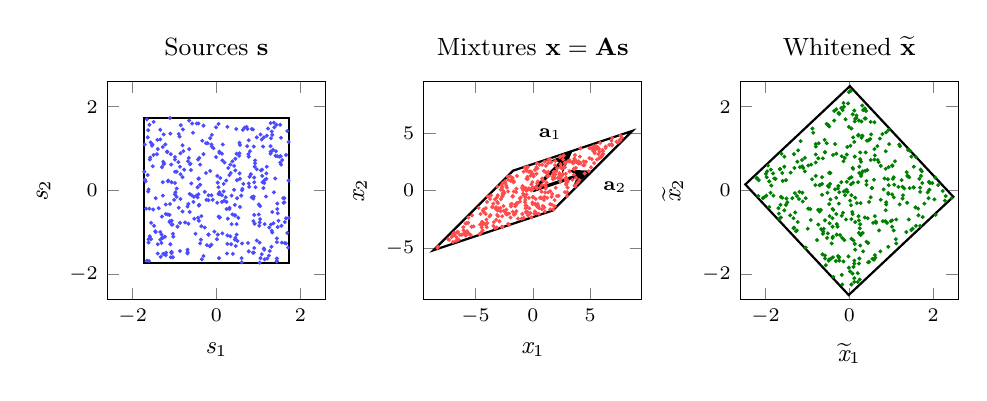
\begin{tikzpicture}
      \begin{groupplot}[group style={group size=3 by 1, horizontal sep=1.25cm},
          width=4.35cm, height=4.35cm, axis equal image, tick label style={font=\scriptsize},
          label style={font=\small}, title style={font=\small}]
        \nextgroupplot[title={Sources $\vect s$}, xlabel={$s_1$}, ylabel={$s_2$}, xmin=-2.6, xmax=2.6, ymin=-2.6, ymax=2.6]
          \addplot[only marks, mark=*, mark size=0.5pt, blue!70] coordinates {(0.43,-0.59) (1.38,1.51) (0.96,-1.19) (-0.95,0.05) (-0.69,-1.41) (1.29,1.61) (-1.71,0.26) (1.11,1.05) (1.03,-0.76) (-0.11,1.05) (-0.68,0.70) (-0.77,0.50) (-0.85,1.56) (-0.19,-0.23) (0.02,-0.29) (0.19,0.67) (1.72,1.16) (1.01,-0.57) (0.42,0.59) (1.69,-1.01) (-0.99,0.18) (-1.18,0.93) (0.39,-1.51) (-1.58,0.79) (-1.61,-1.68) (0.05,1.59) (-0.12,-0.11) (1.45,-0.31) (0.45,0.76) (0.05,0.08) (-0.01,0.80) (-0.87,-1.44) (-1.69,0.22) (-1.07,0.20) (0.67,1.50) (-1.04,-1.59) (-0.45,-0.16) (-1.72,0.45) (1.14,0.18) (-1.20,-1.48) (-0.81,0.32) (1.32,-0.96) (0.03,-1.05) (1.20,1.31) (0.48,-1.05) (0.84,-0.16) (-1.42,0.87) (0.14,0.72) (0.03,0.19) (1.29,1.06) (-0.48,-0.12) (0.34,0.42) (-1.53,1.10) (-0.39,0.62) (-0.61,0.49) (-1.21,-0.33) (1.10,0.20) (-0.42,-0.36) (1.66,0.85) (0.31,-0.41) (0.36,-0.12) (0.48,0.88) (0.61,0.01) (-1.21,-0.56) (-0.21,1.13) (-0.90,-0.41) (-0.34,1.19) (-1.40,0.99) (1.62,-0.18) (-0.99,0.74) (0.60,-1.61) (-0.69,-0.38) (1.30,1.25) (0.56,0.28) (-1.28,0.20) (1.20,0.57) (1.54,0.62) (1.40,0.29) (0.24,-0.27) (-1.23,-1.10) (-1.07,-0.72) (1.48,-0.72) (0.18,-0.24) (-1.11,1.73) (1.33,-0.51) (0.49,-0.18) (0.24,-0.44) (-0.43,0.28) (-0.31,1.55) (-0.90,1.35) (-1.60,-0.43) (1.30,-0.81) (-0.11,1.33) (0.17,-0.02) (-0.62,0.64) (0.87,-1.48) (-1.64,1.27) (-0.44,-0.65) (-1.63,-0.02) (-1.31,-1.05) (1.62,-0.28) (0.55,1.14) (-0.25,1.13) (0.08,-0.09) (1.29,0.93) (-0.54,-0.15) (0.31,-0.44) (0.64,0.16) (-0.50,-1.03) (0.07,-0.64) (0.92,0.72) (1.42,0.94) (-1.21,-1.54) (1.50,0.81) (-1.71,1.10) (0.88,-0.19) (1.08,-1.52) (-1.26,0.63) (-0.28,-0.88) (1.09,0.50) (-1.68,-0.43) (0.45,0.48) (1.02,-0.84) (0.05,-0.08) (0.78,0.09) (-0.95,0.45) (-1.04,-1.03) (-0.47,1.60) (-1.11,-0.73) (-0.53,-0.67) (1.55,-0.84) (0.25,-1.50) (-0.55,-0.27) (-0.79,0.94) (1.57,0.73) (-0.19,-1.05) (1.66,-1.26) (0.05,-0.62) (0.07,0.93) (1.37,-0.04) (0.84,1.47) (0.28,0.54) (-0.25,0.42) (1.31,0.93) (-0.31,0.87) (1.46,-0.54) (-1.49,-0.84) (-0.24,-0.22) (0.07,-0.04) (1.56,-1.24) (-0.86,-0.20) (1.06,0.48) (0.61,-1.26) (0.75,-1.25) (0.45,-1.13) (1.63,-0.75) (-0.58,1.60) (-0.35,-1.64) (-1.03,-1.10) (-1.56,-1.16) (-0.99,-0.09) (1.44,-1.68) (1.18,-0.14) (-1.34,-1.17) (0.36,-0.80) (-0.07,1.01) (0.33,-1.09) (0.55,0.41) (-0.67,-0.32) (1.60,-0.29) (-0.12,1.10) (0.44,-1.17) (0.47,1.47) (-1.10,1.36) (-1.52,0.58) (-0.31,-1.56) (0.91,0.57) (1.09,0.35) (0.80,0.94) (-1.34,-0.99) (1.43,1.57) (1.05,1.34) (1.31,-1.34) (0.08,-0.64) (1.44,-1.62) (-1.57,1.15) (-1.63,1.44) (-1.66,1.70) (-0.86,0.39) (-0.87,0.57) (-1.08,0.62) (0.23,0.24) (-1.60,1.57) (0.31,0.37) (-1.16,-0.57) (0.62,0.04) (-1.66,-1.67) (-0.66,0.78) (1.52,0.67) (0.13,-0.27) (1.08,1.22) (0.55,0.89) (0.38,-0.57) (-1.07,-1.46) (0.26,-1.27) (-1.59,-1.09) (1.04,-0.68) (1.59,-0.18) (1.23,1.48) (-1.56,-0.77) (-0.56,1.38) (-0.63,0.63) (-1.34,1.22) (0.44,-0.34) (1.03,-1.72) (-0.65,0.99) (1.26,-0.88) (1.03,-1.24) (-1.28,1.04) (0.92,0.65) (1.33,-1.00) (-1.05,-0.81) (0.26,1.52) (0.48,-0.80) (0.38,0.70) (-1.40,-1.28) (0.56,1.09) (0.46,-1.32) (1.12,0.06) (1.05,-1.61) (-0.60,0.17) (0.77,1.20) (1.27,-1.44) (1.36,-0.78) (-1.17,0.92) (-1.64,0.37) (0.52,-0.65) (-0.99,0.45) (0.22,-0.16) (1.54,1.26) (-0.42,-0.72) (-0.86,0.89) (-0.15,0.47) (0.54,0.83) (-1.38,-0.42) (-0.41,0.78) (-1.27,0.69) (0.56,-0.39) (1.15,-1.64) (-0.43,1.60) (-0.44,0.74) (0.14,-1.02) (-0.99,0.80) (-0.87,-0.77) (-0.59,-0.11) (-0.15,1.25) (-1.45,-0.18) (0.88,-0.73) (0.27,-0.67) (-0.69,-1.47) (-1.46,-0.97) (0.91,-0.79) (-1.28,-1.13) (-1.27,-1.51) (-1.28,-0.12) (-1.45,-0.99) (1.41,0.83) (-0.80,1.46) (-0.67,-0.79) (1.15,0.25) (0.42,0.02) (-1.08,-1.47) (-0.23,-1.30) (1.33,1.33) (-0.43,-0.09) (0.73,1.06) (-1.40,-1.50) (0.79,0.33) (0.96,1.27) (1.13,1.27) (0.60,-1.71) (-0.45,0.08) (-1.51,-0.45) (0.07,0.90) (0.89,-1.48) (-1.07,-0.81) (-0.81,1.08) (0.13,-0.11) (0.86,-0.16) (1.37,1.62) (-1.30,-0.62) (-1.09,-1.59) (1.04,-0.37) (0.50,-1.20) (0.77,-1.45) (1.72,0.24) (1.52,1.57) (1.19,0.28) (0.96,0.51) (-0.36,-0.61) (0.49,0.25) (-1.09,0.87) (0.90,0.31) (0.89,1.05) (0.77,0.17) (-0.19,-1.05) (-0.42,0.29) (-0.28,-0.03) (-1.62,-1.16) (1.19,0.41) (0.15,1.10) (-0.39,-1.26) (0.17,0.16) (0.77,0.81) (-0.41,-0.34) (1.15,-0.80) (1.45,-0.44) (-0.39,0.14) (-1.25,0.65) (0.90,0.20) (1.71,-1.36) (-1.22,1.10) (0.74,1.47) (1.13,-1.38) (1.46,-0.87) (-1.30,-1.13) (-1.41,1.21) (1.69,1.42) (-1.33,-1.58) (-1.12,-0.58) (0.26,-1.07) (-0.19,-0.11) (0.87,1.46) (-1.07,-1.49) (1.44,-1.14) (-0.98,-0.04) (0.93,0.08) (-1.50,0.85) (-0.09,-0.22) (-1.62,-1.24) (-0.64,-0.51) (-0.65,1.67) (0.76,0.87) (-0.16,-1.33) (-1.54,1.07) (1.72,-0.65) (1.35,0.97) (1.44,-1.69) (-0.88,1.29) (-0.37,-1.17) (-0.95,-0.15) (-1.30,0.56) (-1.62,0.03) (0.01,-1.16) (-1.31,-1.25) (-1.12,-0.75) (1.25,-1.55) (-0.05,-0.98) (-1.10,-1.28) (0.59,-0.12) (-0.81,-0.50) (0.09,0.30) (-0.75,-0.76) (0.06,-1.61) (0.45,-0.59) (0.13,0.88) (-0.36,-0.85) (1.01,-0.33) (1.29,0.88) (-1.11,-0.32) (-1.26,1.34) (-1.34,1.45) (1.66,-0.66) (1.53,0.82) (-0.93,-0.86) (1.63,-1.25) (-1.01,-0.22) (0.02,0.35) (-0.01,1.51) (1.44,-1.23) (-1.59,0.74) (-0.64,-0.08) (0.35,-1.28) (-1.50,1.64) (-0.91,0.68) (-0.12,-1.29) (1.32,1.41) (0.90,-1.37) (1.14,-1.41) (0.90,-0.58) (0.72,1.52) (1.21,-1.62) (0.63,1.45) (0.82,0.39) (-0.69,-1.50) (-1.15,0.24) (0.89,-0.14) (-1.16,0.22) (1.45,0.82) (0.33,0.62)};
          \draw[thick] (axis cs:-1.732,-1.732) rectangle (axis cs:1.732,1.732);
        \nextgroupplot[title={Mixtures $\vect x=\mat A\vect s$}, xlabel={$x_1$}, ylabel={$x_2$}, xmin=-9.5, xmax=9.5, ymin=-9.5, ymax=9.5]
          \addplot[only marks, mark=*, mark size=0.5pt, red!70] coordinates {(-0.91,0.28) (7.29,4.26) (-1.67,0.72) (-1.75,-1.85) (-5.63,-2.80) (7.42,4.20) (-2.64,-3.17) (5.38,3.28) (-0.21,1.30) (2.91,0.82) (0.74,-0.66) (-0.04,-1.04) (2.98,-0.14) (-1.07,-0.61) (-0.85,-0.26) (2.37,1.04) (6.91,4.59) (0.31,1.46) (2.61,1.43) (0.36,2.38) (-1.44,-1.79) (0.44,-1.42) (-3.74,-0.73) (-0.79,-2.37) (-8.25,-4.90) (4.87,1.69) (-0.56,-0.34) (1.95,2.58) (3.19,1.66) (0.34,0.18) (2.38,0.78) (-6.06,-3.19) (-2.73,-3.16) (-1.53,-1.93) (5.82,2.83) (-6.86,-3.67) (-1.39,-1.07) (-2.08,-2.98) (2.81,2.46) (-6.82,-3.87) (-0.64,-1.29) (-0.25,1.67) (-3.10,-0.99) (6.34,3.72) (-2.17,-0.08) (1.20,1.52) (-0.23,-1.96) (2.44,1.00) (0.61,0.24) (5.76,3.64) (-1.32,-1.08) (1.93,1.10) (0.26,-1.95) (1.07,-0.16) (0.25,-0.73) (-3.40,-2.75) (2.80,2.39) (-1.92,-1.20) (5.86,4.16) (-0.62,0.21) (0.38,0.61) (3.61,1.84) (1.26,1.24) (-4.10,-2.98) (2.98,0.72) (-3.04,-2.22) (2.91,0.52) (0.17,-1.81) (2.69,3.06) (0.24,-1.24) (-3.65,-0.42) (-2.53,-1.76) (6.34,3.84) (1.95,1.40) (-1.95,-2.35) (4.10,2.96) (4.93,3.70) (3.67,3.09) (-0.34,0.21) (-5.75,-3.55) (-4.29,-2.85) (0.81,2.25) (-0.36,0.12) (2.97,-0.48) (1.13,2.15) (0.43,0.80) (-0.85,0.04) (-0.01,-0.58) (4.04,0.93) (2.24,-0.46) (-4.48,-3.63) (0.18,1.80) (3.77,1.11) (0.27,0.31) (0.70,-0.59) (-2.69,0.26) (0.52,-2.02) (-2.83,-1.53) (-3.31,-3.27) (-5.75,-3.66) (2.41,2.96) (4.50,2.23) (2.91,0.64) (-0.11,0.07) (5.37,3.51) (-1.52,-1.22) (-0.69,0.19) (1.75,1.43) (-4.11,-2.04) (-1.77,-0.50) (3.98,2.55) (5.65,3.77) (-7.02,-3.95) (5.42,3.81) (-0.13,-2.33) (1.18,1.56) (-2.40,0.64) (-0.62,-1.88) (-3.20,-1.44) (3.67,2.68) (-4.65,-3.79) (2.32,1.37) (-0.48,1.19) (-0.15,0.01) (1.82,1.65) (-0.53,-1.44) (-5.17,-3.12) (3.85,0.65) (-4.41,-2.95) (-3.08,-1.74) (0.57,2.26) (-3.99,-0.99) (-1.91,-1.38) (1.24,-0.64) (5.31,3.86) (-3.55,-1.44) (-0.44,2.07) (-1.75,-0.51) (2.93,1.08) (2.62,2.71) (6.08,3.15) (2.18,1.10) (0.75,-0.09) (5.40,3.55) (1.99,0.25) (1.31,2.39) (-5.51,-3.83) (-1.13,-0.70) (0.02,0.10) (-0.60,1.88) (-2.33,-1.93) (3.57,2.60) (-2.56,-0.04) (-2.26,0.25) (-2.49,-0.23) (1.02,2.52) (3.64,0.44) (-5.63,-2.35) (-5.34,-3.15) (-6.59,-4.27) (-2.26,-2.08) (-2.16,1.20) (1.92,2.21) (-6.19,-3.85) (-1.67,-0.08) (2.90,0.87) (-2.63,-0.44) (2.32,1.51) (-2.31,-1.66) (2.34,2.91) (3.06,0.86) (-2.64,-0.29) (5.34,2.40) (1.90,-0.83) (-1.29,-2.45) (-5.30,-2.17) (3.53,2.39) (3.23,2.53) (4.42,2.54) (-5.65,-3.67) (7.58,4.43) (6.11,3.43) (-1.39,1.28) (-1.76,-0.48) (-1.98,1.26) (0.30,-1.99) (1.06,-1.82) (1.77,-1.63) (-0.55,-1.33) (-0.02,-1.17) (-0.31,-1.55) (1.19,0.71) (1.51,-1.63) (1.75,1.00) (-4.02,-2.88) (1.37,1.28) (-8.32,-4.99) (1.02,-0.54) (5.05,3.71) (-0.55,-0.01) (5.81,3.38) (3.75,1.98) (-0.93,0.20) (-6.53,-3.60) (-3.31,-0.76) (-6.47,-4.28) (0.05,1.41) (2.64,3.01) (6.90,3.94) (-5.42,-3.88) (3.02,0.26) (0.61,-0.64) (0.99,-1.46) (-0.13,0.54) (-3.10,0.34) (1.69,-0.30) (-0.13,1.63) (-1.66,0.82) (0.54,-1.53) (3.79,2.49) (-0.34,1.65) (-4.51,-2.90) (5.07,2.03) (-1.44,0.16) (2.86,1.46) (-6.65,-4.08) (4.39,2.21) (-3.06,-0.41) (2.41,2.30) (-2.73,0.49) (-0.68,-1.02) (5.14,2.74) (-1.77,1.10) (0.38,1.94) (0.41,-1.43) (-2.16,-2.90) (-0.90,0.40) (-0.64,-1.53) (-0.03,0.28) (6.85,4.34) (-2.99,-1.55) (0.97,-0.82) (1.11,0.17) (3.59,1.92) (-4.03,-3.19) (1.51,-0.05) (-0.48,-1.85) (-0.04,0.74) (-2.63,0.65) (3.96,0.75) (1.33,-0.15) (-2.79,-0.75) (0.42,-1.17) (-4.05,-2.52) (-1.50,-1.29) (3.45,0.95) (-3.44,-3.08) (-0.45,1.02) (-1.47,-0.13) (-5.78,-2.85) (-5.84,-3.90) (-0.56,1.03) (-5.95,-3.69) (-7.08,-4.05) (-2.91,-2.68) (-5.87,-3.89) (5.30,3.64) (2.79,-0.14) (-3.70,-2.13) (3.06,2.56) (0.90,0.85) (-6.58,-3.64) (-4.35,-1.75) (6.66,3.99) (-1.13,-0.95) (4.63,2.52) (-7.30,-4.29) (2.56,1.90) (5.71,3.18) (6.07,3.53) (-3.93,-0.51) (-0.67,-0.82) (-4.38,-3.47) (2.83,1.03) (-2.65,0.31) (-4.58,-2.96) (1.63,-0.54) (-0.07,0.14) (1.23,1.56) (7.62,4.37) (-4.46,-3.22) (-6.95,-3.77) (0.95,1.70) (-2.60,-0.20) (-2.81,0.08) (4.15,3.68) (7.76,4.61) (3.20,2.65) (3.45,2.43) (-2.56,-1.34) (1.72,1.22) (0.44,-1.31) (2.73,2.11) (4.93,2.83) (2.06,1.71) (-3.52,-1.43) (0.02,-0.56) (-0.65,-0.59) (-6.70,-4.39) (3.62,2.80) (3.59,1.39) (-4.57,-2.04) (0.80,0.49) (3.96,2.35) (-1.83,-1.16) (-0.10,1.49) (1.58,2.46) (-0.35,-0.64) (-0.57,-1.86) (2.42,2.01) (-0.67,2.05) (0.86,-1.34) (5.88,2.94) (-1.89,0.87) (0.31,2.05) (-6.00,-3.74) (0.80,-1.62) (7.64,4.80) (-7.39,-4.23) (-3.98,-2.82) (-2.68,-0.55) (-0.69,-0.48) (6.12,3.20) (-6.61,-3.63) (-0.54,1.73) (-2.09,-2.00) (2.11,1.95) (-0.44,-2.15) (-0.83,-0.40) (-6.97,-4.48) (-2.81,-1.80) (3.71,0.37) (4.13,2.39) (-4.30,-1.64) (0.13,-2.00) (1.47,2.78) (5.62,3.67) (-2.18,1.20) (2.10,-0.47) (-4.24,-1.90) (-2.35,-2.04) (-0.92,-2.04) (-3.15,-3.21) (-3.45,-1.14) (-6.36,-3.86) (-4.48,-2.99) (-2.15,0.95) (-3.05,-1.09) (-6.04,-3.47) (0.81,1.05) (-3.11,-2.12) (1.09,0.49) (-3.78,-2.26) (-4.73,-1.50) (-0.86,0.31) (2.90,1.13) (-3.26,-1.57) (1.02,1.68) (5.24,3.47) (-3.19,-2.54) (1.50,-1.18) (1.66,-1.23) (1.35,2.67) (5.51,3.88) (-4.43,-2.72) (-0.49,2.01) (-2.67,-2.24) (1.11,0.40) (4.51,1.49) (-0.81,1.65) (-0.98,-2.45) (-1.53,-1.36) (-3.13,-0.58) (1.91,-1.37) (0.21,-1.15) (-4.10,-1.53) (6.86,4.04) (-2.32,0.43) (-1.95,0.87) (0.06,1.23) (5.99,2.96) (-2.43,0.81) (5.60,2.71) (2.79,2.02) (-5.87,-2.87) (-1.59,-2.07) (1.35,1.63) (-1.65,-2.09) (5.37,3.73) (2.53,1.29)};
          \draw[thick] (axis cs:8.660,5.196) -- (axis cs:-1.732,1.732) -- (axis cs:-8.660,-5.196) -- (axis cs:1.732,-1.732) -- cycle;
          \draw[-{Stealth}, very thick] (axis cs:0,0) -- (axis cs:3.464,3.464) node[above left, font=\scriptsize] {$\vect a_1$};
          \draw[-{Stealth}, very thick] (axis cs:0,0) -- (axis cs:5.196,1.732) node[below right, font=\scriptsize] {$\vect a_2$};
        \nextgroupplot[title={Whitened $\widetilde{\vect x}$}, xlabel={$\widetilde x_1$}, ylabel={$\widetilde x_2$}, xmin=-2.6, xmax=2.6, ymin=-2.6, ymax=2.6]
          \addplot[only marks, mark=*, mark size=0.5pt, green!50!black] coordinates {(-0.70,0.14) (0.12,-2.09) (-1.51,0.25) (0.75,0.59) (-0.48,1.53) (0.25,-2.12) (1.45,0.95) (-0.02,-1.57) (-1.25,-0.13) (0.86,-0.73) (1.02,-0.09) (0.94,0.13) (1.75,-0.63) (0.00,0.29) (-0.19,0.20) (0.37,-0.64) (-0.38,-2.06) (-1.11,-0.26) (0.14,-0.75) (-1.91,-0.39) (0.87,0.52) (1.54,0.07) (-1.32,0.87) (1.73,0.46) (-0.01,2.35) (1.12,-1.26) (0.04,0.15) (-1.23,-0.75) (0.25,-0.90) (0.05,-0.11) (0.61,-0.61) (-0.36,1.67) (1.40,0.97) (0.94,0.56) (0.62,-1.60) (-0.36,1.90) (0.24,0.42) (1.59,0.80) (-0.67,-0.92) (-0.16,1.92) (0.84,0.29) (-1.60,-0.17) (-0.74,0.77) (0.10,-1.82) (-1.06,0.46) (-0.68,-0.46) (1.67,0.28) (0.44,-0.66) (0.14,-0.17) (-0.14,-1.69) (0.29,0.40) (0.08,-0.56) (1.92,0.18) (0.75,-0.22) (0.82,0.03) (0.67,1.06) (-0.61,-0.91) (0.08,0.54) (-0.56,-1.78) (-0.49,0.09) (-0.31,-0.17) (0.32,-1.01) (-0.40,-0.44) (0.50,1.23) (0.99,-0.73) (0.39,0.91) (1.12,-0.69) (1.74,0.18) (-1.27,-0.97) (1.27,0.09) (-1.55,0.81) (0.26,0.75) (-0.01,-1.84) (-0.18,-0.60) (1.09,0.70) (-0.42,-1.26) (-0.64,-1.52) (-0.77,-1.18) (-0.34,0.03) (0.13,1.65) (0.29,1.26) (-1.55,-0.47) (-0.27,0.05) (2.06,-0.58) (-1.29,-0.52) (-0.45,-0.21) (-0.46,0.16) (0.54,0.06) (1.36,-0.99) (1.64,-0.43) (0.88,1.39) (-1.48,-0.28) (1.06,-0.95) (-0.10,-0.11) (0.93,-0.08) (-1.65,0.52) (2.12,0.13) (-0.11,0.78) (1.19,1.10) (0.23,1.67) (-1.33,-0.90) (0.45,-1.25) (1.02,-0.71) (-0.09,0.00) (-0.24,-1.59) (0.32,0.46) (-0.51,0.11) (-0.31,-0.56) (-0.34,1.11) (-0.47,0.43) (-0.12,-1.18) (-0.32,-1.68) (-0.19,1.97) (-0.48,-1.64) (2.05,0.31) (-0.74,-0.46) (-1.82,0.41) (1.39,0.36) (-0.39,0.85) (-0.40,-1.13) (0.94,1.45) (0.05,-0.68) (-1.30,-0.06) (-0.06,0.02) (-0.47,-0.61) (1.04,0.28) (0.05,1.48) (1.51,-0.91) (0.31,1.30) (-0.06,0.86) (-1.69,-0.42) (-1.22,0.96) (0.24,0.57) (1.27,-0.19) (-0.58,-1.62) (-0.58,0.92) (-2.06,-0.18) (-0.45,0.42) (0.64,-0.77) (-0.99,-0.91) (0.47,-1.70) (0.22,-0.61) (0.51,-0.16) (-0.25,-1.60) (0.87,-0.47) (-1.41,-0.59) (0.51,1.64) (0.05,0.32) (-0.04,-0.03) (-1.98,-0.12) (0.51,0.73) (-0.39,-1.10) (-1.31,0.54) (-1.40,0.43) (-1.10,0.54) (-1.68,-0.55) (1.59,-0.84) (-0.88,1.48) (-0.01,1.52) (0.33,1.92) (0.68,0.73) (-2.20,0.29) (-0.92,-0.70) (0.17,1.79) (-0.80,0.35) (0.80,-0.73) (-0.98,0.60) (-0.08,-0.69) (0.28,0.69) (-1.32,-0.88) (0.90,-0.77) (-1.12,0.58) (0.74,-1.45) (1.79,-0.31) (1.54,0.57) (-0.86,1.38) (-0.22,-1.06) (-0.51,-1.02) (0.13,-1.27) (0.29,1.65) (0.12,-2.18) (0.23,-1.74) (-1.86,0.12) (-0.48,0.42) (-2.16,0.25) (1.98,0.18) (2.23,-0.01) (2.44,-0.18) (0.92,0.27) (1.07,0.14) (1.25,0.25) (0.04,-0.35) (2.30,-0.13) (0.07,-0.51) (0.46,1.20) (-0.38,-0.46) (0.04,2.38) (1.06,-0.16) (-0.58,-1.55) (-0.26,0.11) (0.12,-1.67) (0.27,-1.06) (-0.65,0.16) (-0.24,1.83) (-1.06,0.78) (0.40,1.90) (-1.20,-0.20) (-1.25,-0.95) (0.20,-1.97) (0.60,1.63) (1.42,-0.69) (0.93,-0.06) (1.87,-0.04) (-0.52,-0.05) (-1.94,0.60) (1.20,-0.33) (-1.50,-0.19) (-1.59,0.23) (1.69,0.07) (-0.17,-1.13) (-1.63,-0.15) (0.21,1.31) (0.93,-1.34) (-0.89,0.27) (0.26,-0.80) (0.12,1.91) (0.41,-1.22) (-1.24,0.69) (-0.74,-0.81) (-1.87,0.50) (0.59,0.26) (0.33,-1.45) (-1.91,0.22) (-1.51,-0.34) (1.53,0.08) (1.48,0.81) (-0.81,0.13) (1.06,0.32) (-0.24,-0.04) (-0.18,-2.01) (-0.18,0.82) (1.28,-0.11) (0.47,-0.27) (0.23,-1.01) (0.73,1.24) (0.88,-0.33) (1.43,0.32) (-0.65,-0.10) (-1.96,0.46) (1.48,-0.94) (0.88,-0.28) (-0.80,0.67) (1.31,0.05) (0.12,1.16) (0.38,0.47) (1.02,-0.86) (0.95,1.11) (-1.12,-0.05) (-0.65,0.32) (-0.51,1.57) (0.39,1.72) (-1.19,-0.03) (0.14,1.71) (-0.13,2.00) (0.87,0.94) (0.37,1.72) (-0.39,-1.59) (1.65,-0.59) (-0.05,1.04) (-0.62,-0.98) (-0.25,-0.31) (-0.24,1.84) (-0.73,1.13) (0.02,-1.93) (0.28,0.35) (0.26,-1.31) (-0.03,2.08) (-0.30,-0.80) (0.24,-1.62) (0.12,-1.74) (-1.62,0.88) (0.41,0.23) (0.79,1.35) (0.63,-0.74) (-1.66,0.51) (0.22,1.33) (1.38,-0.29) (-0.13,-0.02) (-0.70,-0.47) (0.20,-2.18) (0.52,1.34) (-0.31,1.94) (-0.98,-0.43) (-1.18,0.56) (-1.55,0.57) (-1.04,-1.36) (0.05,-2.24) (-0.63,-1.03) (-0.30,-1.05) (-0.14,0.70) (-0.15,-0.53) (1.44,0.06) (-0.40,-0.86) (0.14,-1.41) (-0.40,-0.66) (-0.58,0.91) (0.54,0.06) (0.21,0.20) (0.37,1.96) (-0.53,-1.13) (0.71,-0.95) (-0.59,1.21) (0.02,-0.24) (0.05,-1.15) (0.09,0.52) (-1.36,-0.18) (-1.33,-0.66) (0.41,0.14) (1.39,0.34) (-0.47,-0.78) (-2.17,-0.13) (1.69,-0.03) (0.55,-1.63) (-1.76,0.28) (-1.64,-0.34) (0.17,1.73) (1.91,0.02) (-0.17,-2.24) (-0.14,2.09) (0.42,1.19) (-0.91,0.62) (0.09,0.19) (0.45,-1.71) (-0.26,1.85) (-1.81,-0.12) (0.70,0.68) (-0.58,-0.71) (1.71,0.35) (-0.06,0.21) (0.31,2.03) (0.13,0.81) (1.69,-0.84) (0.10,-1.19) (-0.80,1.11) (1.90,0.21) (-1.67,-0.67) (-0.24,-1.67) (-2.21,0.30) (1.58,-0.40) (-0.54,1.13) (0.60,0.74) (1.37,0.44) (1.21,1.06) (-0.80,0.86) (0.08,1.82) (0.31,1.31) (-1.97,0.32) (-0.63,0.77) (-0.09,1.70) (-0.48,-0.32) (0.26,0.91) (0.18,-0.30) (0.03,1.07) (-1.16,1.18) (-0.71,0.13) (0.57,-0.77) (-0.31,0.88) (-0.93,-0.44) (-0.27,-1.56) (0.60,0.99) (1.89,-0.18) (2.03,-0.21) (-1.63,-0.64) (-0.49,-1.67) (0.09,1.27) (-2.03,-0.16) (0.61,0.84) (0.27,-0.30) (1.11,-1.16) (-1.88,-0.05) (1.70,0.50) (0.43,0.49) (-1.13,0.73) (2.28,-0.24) (1.17,0.09) (-0.80,1.05) (0.08,-1.98) (-1.60,0.42) (-1.79,0.29) (-1.04,-0.18) (0.59,-1.65) (-1.99,0.40) (0.61,-1.54) (-0.28,-0.86) (-0.54,1.59) (1.03,0.59) (-0.71,-0.50) (1.02,0.60) (-0.43,-1.62) (0.23,-0.71)};
          \draw[thick] (-0.014,-2.491) -- (2.480,-0.147) -- (0.014,2.491) -- (-2.480,0.147) -- cycle;
      \end{groupplot}
    \end{tikzpicture}
    \caption{Illustration of ICA with the uniform sources and the mixing matrix $\mat A$ from above (400 samples). Left: the joint pdf of the sources is uniform on an axis-aligned square. Middle: after mixing, the data lie on a parallelogram whose edges point in the directions of the columns $\vect a_1=(2,2)^T$ and $\vect a_2=(3,1)^T$ of $\mat A$ (arrows scaled by $\sqrt3$); $x_1$ and $x_2$ are no longer independent. Right: after centering and whitening, $\widetilde{\vect x}=\mat D^{-\frac12}\mat U^T\vect x$, the data are again uniform on a square, but on a \emph{rotated} one. Only this rotation, i.\,e.\ the orthogonal matrix $\mat{\widetilde A}$, remains to be estimated.}
    \label{fig:ica_whitening}
  \end{figure}

  \textbf{Properties of the whitened observations:}
  \begin{itemize}
    \item Joint pdf of $\widetilde{\vect x}$ is uniform on a square, but on a \emph{rotated} square in general (not aligned with the coordinate axes).
    \item Components are determined except for rotation.
    \item Problem of recovering $\mat{\widetilde A}$ is much simpler.
  \end{itemize}

  \textbf{From the illustration to the estimation algorithm.}
  Figure~\ref{fig:ica_pipeline} summarizes the processing chain: after centering and whitening, only the rotation $\mat{\widetilde A}$ is unknown. Figure~\ref{fig:ica_kurtosis} shows how this rotation is found for the example above: projecting the whitened data onto all unit vectors $\vect w$ and measuring the non-Gaussianity of $\vect w^T\widetilde{\vect x}$ (here by the kurtosis, see Sec.~\ref{sec:ica_kurtosis}) gives maxima exactly in the source directions. Figure~\ref{fig:ica_deflation} shows how the weight vectors are found one after the other under the constraints of the algorithm in Sec.~\ref{sec:ica_algorithm}.

  \begin{figure}[htbp]
    \centering
    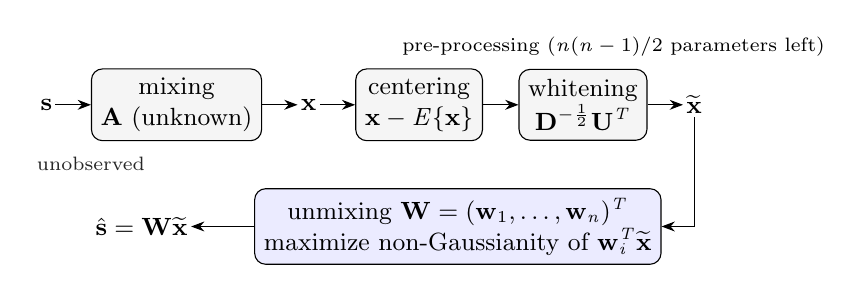
\begin{tikzpicture}[node distance=0.45cm and 0.45cm, font=\small,
        blk/.style={draw, rounded corners, minimum height=0.9cm, align=center, fill=gray!8},
        sig/.style={inner sep=1pt}, >={Stealth}]
      \node[sig] (s) {$\vect s$};
      \node[blk, right=of s] (A) {mixing\\$\mat A$ (unknown)};
      \node[sig, right=of A] (x) {$\vect x$};
      \node[blk, right=of x] (c) {centering\\$\vect x-E\{\vect x\}$};
      \node[blk, right=of c] (w) {whitening\\$\mat D^{-\frac12}\mat U^T$};
      \node[sig, right=of w] (xt) {$\widetilde{\vect x}$};
      \node[blk, fill=blue!8, below=0.9cm of xt, xshift=-3.0cm] (W) {unmixing $\mat W=(\vect w_1,\dots,\vect w_n)^T$\\maximize non-Gaussianity of $\vect w_i^T\widetilde{\vect x}$};
      \node[sig, left=0.8cm of W] (sh) {$\hat{\vect s}=\mat W\widetilde{\vect x}$};
      \draw[->] (s) -- (A); \draw[->] (A) -- (x); \draw[->] (x) -- (c); \draw[->] (c) -- (w); \draw[->] (w) -- (xt);
      \draw[->] (xt) |- (W); \draw[->] (W) -- (sh);
      \node[font=\scriptsize, gray!30!black, below=2pt of A.south west, anchor=north] {unobserved};
      \node[font=\scriptsize, above=1pt of w.north west, anchor=south west, xshift=-1.6cm] {pre-processing ($n(n-1)/2$ parameters left)};
    \end{tikzpicture}
    \caption{Processing chain of the basic ICA estimation algorithm (Sec.~\ref{sec:ica_algorithm}). The sources $\vect s$ and the mixing matrix $\mat A$ are unknown; only $\vect x$ is observed. Centering and whitening turn the unknown mixing into an orthogonal matrix $\mat{\widetilde A}$. The rows $\vect w_i^T$ of the unmixing matrix $\mat W$ are then found one after the other by maximizing the non-Gaussianity of the projections $\vect w_i^T\widetilde{\vect x}$. The estimate $\hat{\vect s}$ equals $\vect s$ up to scale, sign and order.}
    \label{fig:ica_pipeline}
  \end{figure}

  \begin{figure}[htbp]
    \centering
    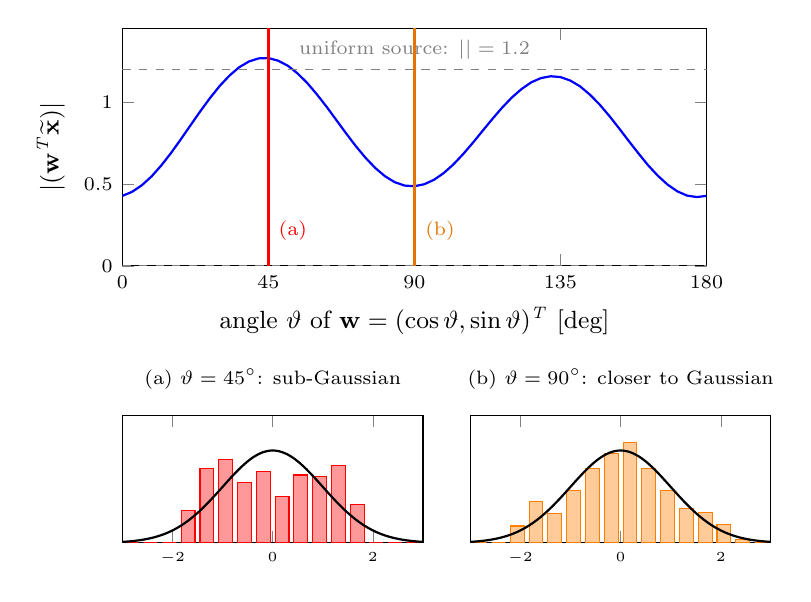
\begin{tikzpicture}
      \begin{axis}[name=kurt, width=9cm, height=4.6cm, xmin=0, xmax=180, ymin=0, ymax=1.45,
          xtick={0,45,90,135,180}, xlabel={angle $\vartheta$ of $\vect w=(\cos\vartheta,\sin\vartheta)^T$ [deg]},
          ylabel={$|\kurt(\vect w^T\widetilde{\vect x})|$}, tick label style={font=\scriptsize}, label style={font=\small}]
        \addplot[thick, blue] coordinates {(0,0.427) (3,0.452) (6,0.492) (9,0.546) (12,0.613) (15,0.689) (18,0.772) (21,0.858) (24,0.943) (27,1.024) (30,1.098) (33,1.161) (36,1.212) (39,1.247) (42,1.266) (45,1.268) (48,1.252) (51,1.221) (54,1.174) (57,1.115) (60,1.045) (63,0.969) (66,0.888) (69,0.807) (72,0.729) (75,0.658) (78,0.596) (81,0.546) (84,0.510) (87,0.490) (90,0.486) (93,0.498) (96,0.525) (99,0.566) (102,0.619) (105,0.682) (108,0.751) (111,0.824) (114,0.896) (117,0.965) (120,1.027) (123,1.079) (126,1.120) (129,1.146) (132,1.157) (135,1.152) (138,1.131) (141,1.096) (144,1.046) (147,0.986) (150,0.916) (153,0.841) (156,0.763) (159,0.687) (162,0.614) (165,0.550) (168,0.496) (171,0.455) (174,0.429) (177,0.420) (180,0.427)};
        \addplot[dashed, gray] coordinates {(0,1.2) (180,1.2)} node[pos=0.5, above, font=\scriptsize] {uniform source: $|\kurt|=1.2$};
        \addplot[dashed, gray] coordinates {(0,0) (180,0)};
        \addplot[red, thick] coordinates {(45,0) (45,1.45)} node[pos=0.15, right, font=\scriptsize] {(a)};
        \addplot[orange!90!black, very thick] coordinates {(90,0) (90,1.45)} node[pos=0.15, right, font=\scriptsize] {(b)};
      \end{axis}
      \begin{axis}[name=ha, at={(kurt.south west)}, anchor=north west, yshift=-1.9cm, width=5.4cm, height=3.2cm,
          xmin=-3, xmax=3, ymin=0, ymax=0.55, title={(a) $\vartheta=45^\circ$: sub-Gaussian}, title style={font=\scriptsize},
          tick label style={font=\tiny}, ytick=\empty]
        \addplot[ybar, bar width=5pt, fill=red!40, draw=red] coordinates {(-2.812,0.000) (-2.438,0.000) (-2.062,0.000) (-1.688,0.140) (-1.312,0.320) (-0.938,0.360) (-0.562,0.260) (-0.188,0.307) (0.188,0.200) (0.562,0.293) (0.938,0.287) (1.312,0.333) (1.688,0.167) (2.062,0.000) (2.438,0.000) (2.812,0.000)};
        \addplot[smooth, thick, black, domain=-3:3, samples=50] {exp(-x^2/2)/sqrt(2*pi)};
      \end{axis}
      \begin{axis}[at={(ha.east)}, anchor=west, xshift=0.6cm, width=5.4cm, height=3.2cm,
          xmin=-3, xmax=3, ymin=0, ymax=0.55, title={(b) $\vartheta=90^\circ$: closer to Gaussian}, title style={font=\scriptsize},
          tick label style={font=\tiny}, ytick=\empty]
        \addplot[ybar, bar width=5pt, fill=orange!40, draw=orange] coordinates {(-2.812,0.000) (-2.438,0.000) (-2.062,0.073) (-1.688,0.180) (-1.312,0.127) (-0.938,0.227) (-0.562,0.320) (-0.188,0.387) (0.188,0.433) (0.562,0.320) (0.938,0.227) (1.312,0.147) (1.688,0.133) (2.062,0.080) (2.438,0.013) (2.812,0.000)};
        \addplot[smooth, thick, black, domain=-3:3, samples=50] {exp(-x^2/2)/sqrt(2*pi)};
      \end{axis}
    \end{tikzpicture}
    \caption{Why maximizing non-Gaussianity finds the independent components (whitened data of Fig.~\ref{fig:ica_whitening}). Top: absolute kurtosis of the projection $\vect w^T\widetilde{\vect x}$ for all unit vectors $\vect w$. It is maximal (close to $1.2$, the value of a single uniform source) when $\vect w$ points along a source direction, and minimal halfway in between, where the projection is a sum of both sources and, by the central limit theorem, more Gaussian. Bottom: histograms of the projection (bars) against the standard normal pdf (black) at (a) a maximum and (b) a minimum of $|\kurt|$.}
    \label{fig:ica_kurtosis}
  \end{figure}

  \begin{figure}[htbp]
    \centering
    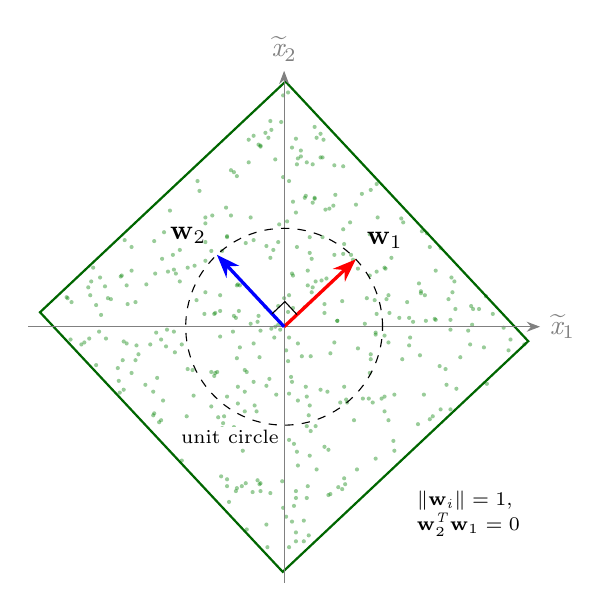
\begin{tikzpicture}[scale=1.25, >={Stealth}]
      \foreach \p in {(-0.70,0.14),(0.12,-2.09),(-1.51,0.25),(0.75,0.59),(-0.48,1.53),(0.25,-2.12),(1.45,0.95),(-0.02,-1.57),(-1.25,-0.13),(0.86,-0.73),(1.02,-0.09),(0.94,0.13),(1.75,-0.63),(0.00,0.29),(-0.19,0.20),(0.37,-0.64),(-0.38,-2.06),(-1.11,-0.26),(0.14,-0.75),(-1.91,-0.39),(0.87,0.52),(1.54,0.07),(-1.32,0.87),(1.73,0.46),(-0.01,2.35),(1.12,-1.26),(0.04,0.15),(-1.23,-0.75),(0.25,-0.90),(0.05,-0.11),(0.61,-0.61),(-0.36,1.67),(1.40,0.97),(0.94,0.56),(0.62,-1.60),(-0.36,1.90),(0.24,0.42),(1.59,0.80),(-0.67,-0.92),(-0.16,1.92),(0.84,0.29),(-1.60,-0.17),(-0.74,0.77),(0.10,-1.82),(-1.06,0.46),(-0.68,-0.46),(1.67,0.28),(0.44,-0.66),(0.14,-0.17),(-0.14,-1.69),(0.29,0.40),(0.08,-0.56),(1.92,0.18),(0.75,-0.22),(0.82,0.03),(0.67,1.06),(-0.61,-0.91),(0.08,0.54),(-0.56,-1.78),(-0.49,0.09),(-0.31,-0.17),(0.32,-1.01),(-0.40,-0.44),(0.50,1.23),(0.99,-0.73),(0.39,0.91),(1.12,-0.69),(1.74,0.18),(-1.27,-0.97),(1.27,0.09),(-1.55,0.81),(0.26,0.75),(-0.01,-1.84),(-0.18,-0.60),(1.09,0.70),(-0.42,-1.26),(-0.64,-1.52),(-0.77,-1.18),(-0.34,0.03),(0.13,1.65),(0.29,1.26),(-1.55,-0.47),(-0.27,0.05),(2.06,-0.58),(-1.29,-0.52),(-0.45,-0.21),(-0.46,0.16),(0.54,0.06),(1.36,-0.99),(1.64,-0.43),(0.88,1.39),(-1.48,-0.28),(1.06,-0.95),(-0.10,-0.11),(0.93,-0.08),(-1.65,0.52),(2.12,0.13),(-0.11,0.78),(1.19,1.10),(0.23,1.67),(-1.33,-0.90),(0.45,-1.25),(1.02,-0.71),(-0.09,0.00),(-0.24,-1.59),(0.32,0.46),(-0.51,0.11),(-0.31,-0.56),(-0.34,1.11),(-0.47,0.43),(-0.12,-1.18),(-0.32,-1.68),(-0.19,1.97),(-0.48,-1.64),(2.05,0.31),(-0.74,-0.46),(-1.82,0.41),(1.39,0.36),(-0.39,0.85),(-0.40,-1.13),(0.94,1.45),(0.05,-0.68),(-1.30,-0.06),(-0.06,0.02),(-0.47,-0.61),(1.04,0.28),(0.05,1.48),(1.51,-0.91),(0.31,1.30),(-0.06,0.86),(-1.69,-0.42),(-1.22,0.96),(0.24,0.57),(1.27,-0.19),(-0.58,-1.62),(-0.58,0.92),(-2.06,-0.18),(-0.45,0.42),(0.64,-0.77),(-0.99,-0.91),(0.47,-1.70),(0.22,-0.61),(0.51,-0.16),(-0.25,-1.60),(0.87,-0.47),(-1.41,-0.59),(0.51,1.64),(0.05,0.32),(-0.04,-0.03),(-1.98,-0.12),(0.51,0.73),(-0.39,-1.10),(-1.31,0.54),(-1.40,0.43),(-1.10,0.54),(-1.68,-0.55),(1.59,-0.84),(-0.88,1.48),(-0.01,1.52),(0.33,1.92),(0.68,0.73),(-2.20,0.29),(-0.92,-0.70),(0.17,1.79),(-0.80,0.35),(0.80,-0.73),(-0.98,0.60),(-0.08,-0.69),(0.28,0.69),(-1.32,-0.88),(0.90,-0.77),(-1.12,0.58),(0.74,-1.45),(1.79,-0.31),(1.54,0.57),(-0.86,1.38),(-0.22,-1.06),(-0.51,-1.02),(0.13,-1.27),(0.29,1.65),(0.12,-2.18),(0.23,-1.74),(-1.86,0.12),(-0.48,0.42),(-2.16,0.25),(1.98,0.18),(2.23,-0.01),(2.44,-0.18),(0.92,0.27),(1.07,0.14),(1.25,0.25),(0.04,-0.35),(2.30,-0.13),(0.07,-0.51),(0.46,1.20),(-0.38,-0.46),(0.04,2.38),(1.06,-0.16),(-0.58,-1.55),(-0.26,0.11),(0.12,-1.67),(0.27,-1.06),(-0.65,0.16),(-0.24,1.83),(-1.06,0.78),(0.40,1.90),(-1.20,-0.20),(-1.25,-0.95),(0.20,-1.97),(0.60,1.63),(1.42,-0.69),(0.93,-0.06),(1.87,-0.04),(-0.52,-0.05),(-1.94,0.60),(1.20,-0.33),(-1.50,-0.19),(-1.59,0.23),(1.69,0.07),(-0.17,-1.13),(-1.63,-0.15),(0.21,1.31),(0.93,-1.34),(-0.89,0.27),(0.26,-0.80),(0.12,1.91),(0.41,-1.22),(-1.24,0.69),(-0.74,-0.81),(-1.87,0.50),(0.59,0.26),(0.33,-1.45),(-1.91,0.22),(-1.51,-0.34),(1.53,0.08),(1.48,0.81),(-0.81,0.13),(1.06,0.32),(-0.24,-0.04),(-0.18,-2.01),(-0.18,0.82),(1.28,-0.11),(0.47,-0.27),(0.23,-1.01),(0.73,1.24),(0.88,-0.33),(1.43,0.32),(-0.65,-0.10),(-1.96,0.46),(1.48,-0.94),(0.88,-0.28),(-0.80,0.67),(1.31,0.05),(0.12,1.16),(0.38,0.47),(1.02,-0.86),(0.95,1.11),(-1.12,-0.05),(-0.65,0.32),(-0.51,1.57),(0.39,1.72),(-1.19,-0.03),(0.14,1.71),(-0.13,2.00),(0.87,0.94),(0.37,1.72),(-0.39,-1.59),(1.65,-0.59),(-0.05,1.04),(-0.62,-0.98),(-0.25,-0.31),(-0.24,1.84),(-0.73,1.13),(0.02,-1.93),(0.28,0.35),(0.26,-1.31),(-0.03,2.08),(-0.30,-0.80),(0.24,-1.62),(0.12,-1.74),(-1.62,0.88),(0.41,0.23),(0.79,1.35),(0.63,-0.74),(-1.66,0.51),(0.22,1.33),(1.38,-0.29),(-0.13,-0.02),(-0.70,-0.47),(0.20,-2.18),(0.52,1.34),(-0.31,1.94),(-0.98,-0.43),(-1.18,0.56),(-1.55,0.57),(-1.04,-1.36),(0.05,-2.24),(-0.63,-1.03),(-0.30,-1.05),(-0.14,0.70),(-0.15,-0.53),(1.44,0.06),(-0.40,-0.86),(0.14,-1.41),(-0.40,-0.66),(-0.58,0.91),(0.54,0.06),(0.21,0.20),(0.37,1.96),(-0.53,-1.13),(0.71,-0.95),(-0.59,1.21),(0.02,-0.24),(0.05,-1.15),(0.09,0.52),(-1.36,-0.18),(-1.33,-0.66),(0.41,0.14),(1.39,0.34),(-0.47,-0.78),(-2.17,-0.13),(1.69,-0.03),(0.55,-1.63),(-1.76,0.28),(-1.64,-0.34),(0.17,1.73),(1.91,0.02),(-0.17,-2.24),(-0.14,2.09),(0.42,1.19),(-0.91,0.62),(0.09,0.19),(0.45,-1.71),(-0.26,1.85),(-1.81,-0.12),(0.70,0.68),(-0.58,-0.71),(1.71,0.35),(-0.06,0.21),(0.31,2.03),(0.13,0.81),(1.69,-0.84),(0.10,-1.19),(-0.80,1.11),(1.90,0.21),(-1.67,-0.67),(-0.24,-1.67),(-2.21,0.30),(1.58,-0.40),(-0.54,1.13),(0.60,0.74),(1.37,0.44),(1.21,1.06),(-0.80,0.86),(0.08,1.82),(0.31,1.31),(-1.97,0.32),(-0.63,0.77),(-0.09,1.70),(-0.48,-0.32),(0.26,0.91),(0.18,-0.30),(0.03,1.07),(-1.16,1.18),(-0.71,0.13),(0.57,-0.77),(-0.31,0.88),(-0.93,-0.44),(-0.27,-1.56),(0.60,0.99),(1.89,-0.18),(2.03,-0.21),(-1.63,-0.64),(-0.49,-1.67),(0.09,1.27),(-2.03,-0.16),(0.61,0.84),(0.27,-0.30),(1.11,-1.16),(-1.88,-0.05),(1.70,0.50),(0.43,0.49),(-1.13,0.73),(2.28,-0.24),(1.17,0.09),(-0.80,1.05),(0.08,-1.98),(-1.60,0.42),(-1.79,0.29),(-1.04,-0.18),(0.59,-1.65),(-1.99,0.40),(0.61,-1.54),(-0.28,-0.86),(-0.54,1.59),(1.03,0.59),(-0.71,-0.50),(1.02,0.60),(-0.43,-1.62),(0.23,-0.71)} {\fill[green!50!black, opacity=0.4] \p circle (0.6pt);}
      \draw[thick, green!40!black] (-0.014,-2.491) -- (2.480,-0.147) -- (0.014,2.491) -- (-2.480,0.147) -- cycle;
      \draw[->, gray] (-2.6,0) -- (2.6,0) node[right] {$\widetilde x_1$};
      \draw[->, gray] (0,-2.6) -- (0,2.6) node[above] {$\widetilde x_2$};
      \draw[dashed] (0,0) circle (1);
      \node[font=\scriptsize, fill=white, inner sep=1pt] at (-0.55,-1.12) {unit circle};
      \draw[->, very thick, red] (0,0) -- (0.729,0.685) node[above right, black] {$\vect w_1$};
      \draw[->, very thick, blue] (0,0) -- (-0.683,0.731) node[above left, black] {$\vect w_2$};
      \draw (0.131,0.123) -- (0.008,0.255) -- (-0.123,0.131);
      \node[font=\scriptsize, align=left, anchor=west] at (1.25,-1.9) {$\|\vect w_i\|=1$,\\$\vect w_2^T\vect w_1=0$};
    \end{tikzpicture}
    \caption{The estimation algorithm of Sec.~\ref{sec:ica_algorithm} in the whitened space ($n=2$). In each iteration, $\vect w_i$ is searched on the unit circle (dashed), i.\,e.\ subject to $\|\vect w_i\|=1$. The first vector $\vect w_1$ converges to a direction of maximal non-Gaussianity, which is aligned with an edge of the rotated square and thus with one source. The second vector $\vect w_2$ must be orthogonal to $\vect w_1$; in two dimensions this leaves only one direction (up to sign), which is the remaining source direction. Stacking $\vect w_1^T,\vect w_2^T$ as rows gives $\mat W$.}
    \label{fig:ica_deflation}
  \end{figure}
  
 
\subsection{Properties of ICA}
 \textbf {Assumptions for the ICA model:}
  \begin{itemize}
    \item We assume that the $s_j$ are mutually independent.            
    \item The $s_j$ have to be non-Gaussian in order to determine them from the $x_i$.
    \item For simplicity, we assume that $\mat A$ is square, i.\,e.\ from now on $m=n$.
  \end{itemize}
 \textbf {Ambiguities of the ICA model:}
  \begin{itemize} 
    \item The $s_j$ are defined only up to a multiplicative constant.
    \item The $s_j$ are not ordered.
  \end{itemize}
 Writing the ICA model in terms of the columns of $\mat A$:
  \begin{displaymath}
    \vect x = \sum_{i=1}^n \vect a_i s_i            
  \end{displaymath}
  
  \begin{itemize}
    \item Any \textbf        {scalar multiplier} for $s_i$ can be eliminated by scaling $\vect a_i$ appropriately.            
    \item The matrix $\mat A$ can be adapted to restrict the $s_i$ to have \textbf        {unit variance}.            
    \item This still leaves the ambiguity of the \textbf        {sign}: \\
      multiplying $s_i$ by $\pm 1$ does not affect the model.            
    \item This ambiguity is usually \textbf        {insignificant} in most applications.
  \end{itemize}
 
 \textbf        {Ambiguity of the ordering:}
  \begin{displaymath}
    \vect x = \sum_{i=1}^n \vect a_i s_i
  \end{displaymath}
  \begin{itemize}
    \item As both $\vect s$ and $\mat A$ are unknown we can change the order of the summation.            
    \item Formalization using a \textbf        {permutation matrix $\mat P$}:
      \begin{displaymath}
        \vect x = \underbrace{\mat A \mat P}_{\mat A^{\ast}} \underbrace{\mat P^{-1} \vect s}_{\vect s^{\ast}}            
      \end{displaymath}
    \item $\mat A^{\ast}$ is just a new mixing matrix to be solved.
  \end{itemize}
 
\subsection{Basic Principle of ICA}

  So far, if we know $\mat A$, we could compute its inverse $\mat A^{-1}$ to obtain the independent components. Consider a linear combination of $x_i$ with a weight vector $\vect w$:
  \begin{displaymath}
    y = \vect w^T \vect x
  \end{displaymath}
  \vspace{0.5\baselineskip}

  Clearly, $y$ equals one of the independent components if $\vect w$ is one row of $\mat A^{-1}$.Change in variables:

  \begin{displaymath}
    \vect z = \mat A^T \vect w
  \end{displaymath}
  
  Applied to the linear combination:
 \begin{displaymath}
    y = \vect w^T \vect x = \vect w^T \mat A \vect s = \vect z^T \vect s
  \end{displaymath}
 
 \textbf{Result from the Central Limit Theorem:}

  \begin{itemize}
    \item The sum of a number of independent random variables tends toward a normal distribution.
    \item $\vect z^T \vect s$ is \textit{typically} more Gaussian than any of the $s_i$.
    \item $\vect z^T \vect s$ is \textit{least Gaussian} when it equals one of the $s_i$.
  \end{itemize}
 
 \textbf {Key principle of ICA:}         

  Maximizing the non-Gaussianity of $\vect w^T \vect x$ results in the independent components!\\[0.3cm]

 \textbf {Reasons for the importance of the non-Gaussianity:}             
 \begin{itemize}
    \item In case of Gaussian random variables, the ICA model can only be estimated up to an orthogonal transformation.                 
     \textbf{Note:}\\
      \quad If just one of the components is Gaussian, ICA still works.                             
    \item The Gaussian is the \textit{most random} distribution within the family of pdfs with given mean and variance.             
    \item Therefore, it is the least informative pdf with respect to the underlying data.
  \end{itemize}
  
  Distributions that have the \textit{least resemblance} to the Gaussian reveal more structure associated with the data.
 
\subsubsection{Importance of Non-Gaussianity}
  The \textit{randomness} can be measured using the concept of entropy from Shannon's information theory:
  \begin{itemize}
    \item Entropy is a measure of the uncertainty of an event, or the randomness of a measure.
  \end{itemize}
  \vspace{0.5\baselineskip}

\subsubsection{Differential Entropy}
  
  The \textit{differential entropy} of a continuous random variable $X$ with density $p(x)$ is defined as
    \begin{displaymath}
      H(x) = - \int p(x) \log p(x) \,\mathsf{d}x
    \end{displaymath}
  
\textbf{Theorem:}\\
    The Gaussian maximizes the entropy over all distributions with the same mean and the same covariance.\\
 \textbf {Proof:}   \\         

  \begin{itemize}
    \item Let $x$ be the random variable, $p(x)$ the pdf that has the highest randomness. \item Rewrite moments $M_i$ equations using a set of polynomials $\{ r_i(x) \}$:
      \begin{displaymath}
        \int p(x) r_i(x) \,\mathsf{d}x = M_i ~,~\mbox{where}~M_i~\mbox{are called moments}. \end{displaymath} 
    \item Using $r_0(x) \equiv 1$, $M_0 = 1$ constrains $p(x)$ to be a pdf.
  \end{itemize}
 
 \textbf{Lagrangian functional for the maximum entropy problem:}

  {\small
  \begin{displaymath}
    \argmin_{p(x)} \mathcal L(p) \equiv 
    \argmin_{p(x)} \int p(x) \log p(x) \,\mathsf{d}x - \sum_{i = 0}^N \lambda_i \left( \int p(x) r_i(x) \,\mathsf{d}x - M_i \right)
  \end{displaymath}
  }
  Taking the functional derivative with respect to $p(x)$ (G\^{a}teaux derivative) and setting it to zero:
%
  {\small
  \begin{displaymath}
    \frac{\delta \mathcal L}{\delta p} = \log p(x) + 1 - \sum_{i=0}^N \lambda_i r_i(x) \stackrel{!}{=} 0
  \end{displaymath}
  }
              
%  
  yields the family of exponential distributions:
%
  {\small
  \begin{displaymath}
    p(x) = \exp \left( -1 + \sum_{i=0}^N \lambda_i r_i(x) \right)
  \end{displaymath}
  } 
  Result for using first and second moments for mean $\mu$ and variance $\sigma^2$:
  \begin{displaymath}
    p(x) = e^{-(1 - \lambda_0 - \lambda_1 x - \lambda_2 (x-\mu)^2)}
  \end{displaymath}
  Plug the form into the constraints:
  \begin{eqnarray*}
    \int e^{-(1 - \lambda_0 - \lambda_1 x - \lambda_2 (x-\mu)^2)} \,\mathsf{d}x &=& 1 \\
    \int x e^{-(1 - \lambda_0 - \lambda_1 x - \lambda_2 (x-\mu)^2)} \,\mathsf{d}x &=& \mu \\
    \int (x-\mu)^2 e^{-(1 - \lambda_0 - \lambda_1 x - \lambda_2 (x-\mu)^2)} \,\mathsf{d}x &=& \sigma^2
  \end{eqnarray*}
 
  Integrate analytically (non-trivial) and solve for Lagrangian multipliers:
  \begin{eqnarray*}
    \lambda_0 &=& 1 - \frac{1}{2} \log(2 \pi \sigma^2 ) \\
    \lambda_1 &=& 0 \\
    \lambda_2 &=& - \frac{1}{2 \sigma^2}  
  \end{eqnarray*}
   
  Insert the results into the form of $p(x)$:
  \begin{eqnarray*}
    p(x) &=& e^{-(1 - \lambda_0 - \lambda_1 x - \lambda_2 (x-\mu)^2)} \\
         &=& e^{-\frac{1}{2} \log(2 \pi \sigma^2)} e^{-\frac{(x-\mu)^2}{2 \sigma^2}} \\
         &=& \frac{1}{\sqrt{2 \pi} \sigma} e^{- \frac{(x-\mu)^2}{2 \sigma^2}}
  \end{eqnarray*}
  
\subsection{ICA Estimation Algorithm}\label{sec:ica_algorithm}

 \textbf{Basic ICA Estimation Algorithm:}

  \begin{centernss}
    \begin{struktogramm}(105,50)
      \assign{Apply centering transform}
      \assign{Apply whitening transform}
      \assign{$i \gets 1$}
      \until{$i > n$~ ($n$: number of independent components)}
        \assign{Take a random vector $\vect w_i$}
        \assign{Maximize non-Gaussianity of $\vect w_i^T \vect{\tilde x}$ subject to $\| \vect w_i \| = 1$ and $\vect w_j^T \vect w_i = 0$, $j<i$}
        \assign{$i \gets i+1$}
      \untilend
      \assign{Use weight matrix $\mat W = \left( \vect w_1, \vect w_2, \ldots, \vect w_n \right)^T$ to compute $\hat{\vect s}=\mat W\vect{\tilde x}$}
      \assign{Output: independent components $\hat{\vect s}$ (up to scale, sign and order)}
    \end{struktogramm}
  \end{centernss}
  \vspace{0.3cm}
  
 \textbf {Notes:}\\

  \begin{itemize}
    \item Estimation by maximizing non-Gaussianity of independent components.            
    \item There exist equivalent algorithms for solving the ICA:
      \begin{itemize}
        \item Gradient descent methods
        \item Fast ICA
      \end{itemize}
                 
    \item Relation to Projection Pursuit approach (Friedman and Tukey, 1974):
      \begin{itemize}
        \item Projection Pursuit is a method for visualization and exploratory data analysis.
        \item Attempts to show clustering structure by finding \textit{interesting} projections.
        \item Interestingness is usually measured by non-Gaussianity.
      \end{itemize}
  \end{itemize}
 
\subsection{Measures of Non-Gaussianity}

these measures of gaussianity will be seen in other lectures, so it is good to understand them.  

  \begin{itemize}
    \item So far, we have seen that the key principle in estimating independent components is the non-Gaussianity.            
    \item In order to optimize the independent components, we need a quantitative measure of non-Gaussianity.
  \end{itemize}
 
  Consider the random variable $y$ and assume that it has zero mean and unit variance (enforced by pre-processing).  We will consider three measures of non-Gaussianity:

  \begin{itemize}
    \item\textbf        {Kurtosis}
    \item\textbf        {Negentropy}
    \item\textbf        {Mutual Information}
  \end{itemize}
          
\subsubsection{Kurtosis}\label{sec:ica_kurtosis}

\textbf{Definition}
 
   The \textbf {\textit{Kurtosis}} of $y$ is defined as:
    \begin{displaymath}
      \kurt(y) = E \{ y^4 \} - 3 \left( E\{ y^2 \} \right)^2
    \end{displaymath}
%    
    Since $y$ has unit variance, the equation simplifies to:
    \begin{displaymath}
      \kurt(y) = E \{ y^4 \} - 3
    \end{displaymath}    
    Additivity (for independent random variables $y_1, y_2$) and homogeneity:
    \begin{eqnarray*}
      \kurt(y_1 + y_2) &=& \kurt(y_1) + \kurt(y_2) \\
      \kurt(\alpha y) &=& \alpha^4 \kurt(y) ~, \quad \alpha \in \real
    \end{eqnarray*}
Kurtosis for a Gaussian distribution:
  
  \begin{itemize}
    \item The $n$-th central moment of a Gaussian distribution $p(y) = {\mathcal{N}}(y ; \mu, \sigma^2)$ with mean $\mu$ and variance $\sigma^2$ is:
      \begin{eqnarray*}
        E \{ (y - \mu)^n \} = \begin{cases}
                                (n-1) !! \cdot \sigma^n \quad &, ~n~ \mbox{even} \\
                                0 \quad &, ~n~ \mbox{odd}
                              \end{cases}
      \end{eqnarray*}
     \textbf{Note:}
      $(n-1)!!$ denotes the double factorial; for even $n$ we have $(n-1)!! = 1\cdot 3\cdot \dots \cdot (n-1)$.
    \item Thus, for a zero mean, unit variance random variable $y$ that is normally distributed:
      \begin{displaymath}
        \kurt(y) = 0
      \end{displaymath}
  \end{itemize}
 \textbf {Properties of Kurtosis:}

Figure~\ref{fig:kurtosis_densities} compares a sub-Gaussian, the Gaussian, and a super-Gaussian density.

  \begin{figure}[htbp]
    \centering
    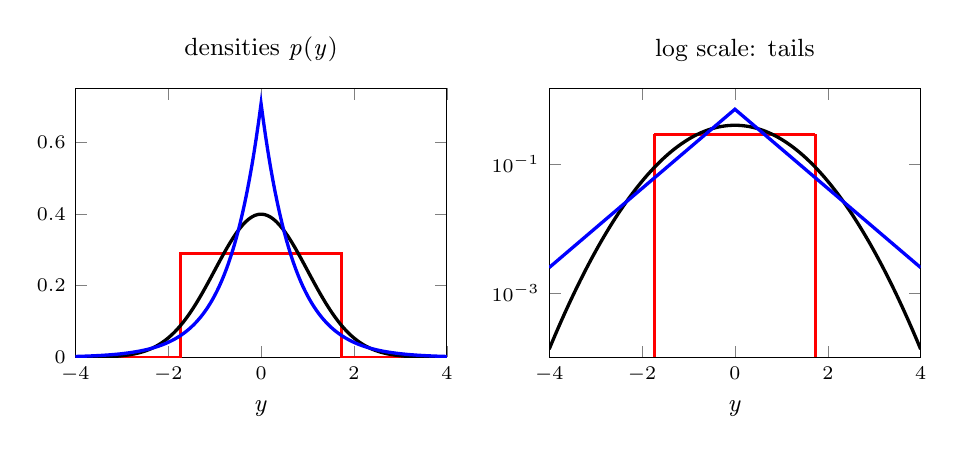
\begin{tikzpicture}
      \begin{groupplot}[group style={group size=2 by 1, horizontal sep=1.3cm}, width=6.3cm, height=5cm,
          xmin=-4, xmax=4, xlabel={$y$}, tick label style={font=\scriptsize}, label style={font=\small}, title style={font=\small},
          legend style={font=\scriptsize, draw=none, fill=white, fill opacity=0.8, text opacity=1}, legend cell align=left]
        \nextgroupplot[title={densities $p(y)$}, ymin=0, ymax=0.75, legend to name=kurtleg, legend columns=3]
          \addplot[red, very thick, const plot] coordinates {(-4,0) (-1.7321,0.2887) (1.7321,0) (4,0)};
          \addlegendentry{uniform: $\kurt=-1.2$}
          \addplot[black, very thick, domain=-4:4, samples=121] {exp(-x^2/2)/sqrt(2*pi)};
          \addlegendentry{Gaussian: $\kurt=0$}
          \addplot[blue, very thick, domain=-4:4, samples=161] {exp(-sqrt(2)*abs(x))/sqrt(2)};
          \addlegendentry{Laplace: $\kurt=3$}
        \nextgroupplot[title={log scale: tails}, ymode=log, ymin=1e-4, ymax=1.5, ylabel={}]
          \addplot[red, very thick, const plot] coordinates {(-1.7321,0.2887) (1.7321,0.2887)};
          \draw[red, very thick] (axis cs:-1.7321,1e-4) -- (axis cs:-1.7321,0.2887) (axis cs:1.7321,1e-4) -- (axis cs:1.7321,0.2887);
          \addplot[black, very thick, domain=-4:4, samples=121] {exp(-x^2/2)/sqrt(2*pi)};
          \addplot[blue, very thick, domain=-4:4, samples=161] {exp(-sqrt(2)*abs(x))/sqrt(2)};
      \end{groupplot}
    \end{tikzpicture}

    \ref*{kurtleg}
    \caption{Three zero-mean, unit-variance densities with different kurtosis. The \emph{sub-Gaussian} uniform density ($\kurt=-1.2$) is flat and has no tails. The \emph{super-Gaussian} Laplace density $p(y)=\frac{1}{\sqrt2}e^{-\sqrt2|y|}$ ($\kurt=3$) has a sharp peak at zero and heavy tails: on the log scale (right) its tails decay only linearly, while the Gaussian ones decay quadratically. Since $\kurt$ measures the fourth moment relative to a Gaussian of the same variance, $|\kurt(y)|$ (or $\kurt(y)^2$) can serve as a measure of non-Gaussianity.}
    \label{fig:kurtosis_densities}
  \end{figure}

  \begin{itemize}
    \item Kurtosis is zero for a Gaussian random variable.            
    \item For most (but not all) non-Gaussian random variables, Kurtosis is nonzero.           \item Kurtosis can be positive or negative.            
    \item Typically, non-Gaussianity is measured as:
      \begin{itemize}
        \item\textbf        {$| \kurt(y) |$} ~ or
        \item\textbf        {$\kurt(y)^2$}
      \end{itemize}
  \end{itemize}
   
\textbf{Example}
        \textbf{\small \hspace{.5cm} Subgaussian pdf} (uniform, zero mean, unit variance), $\kurt(y)<0$:
        \begin{displaymath}
          p(y) = \begin{cases}
                   \frac{1}{2\sqrt{3}} \quad &, ~\mbox{if}~|y| \leq \sqrt{3} \\
                   0 \quad &, ~\mbox{otherwise}
                 \end{cases}
        \end{displaymath}
      
       \textbf  {\small \hspace{.5cm} Supergaussian pdf} (Laplace, zero mean, unit variance), $\kurt(y)>0$:
        {\footnotesize
        \begin{displaymath}
          p(y) = \frac{1}{\sqrt{2}} \exp(-\sqrt{2} |y|)
        \end{displaymath}
        }
   
  \begin{itemize}
    \item Consider 2-D case using the linear combination:
      \begin{eqnarray*}
        y        &=& \vect w^T \vect x = \vect w^T \mat A \vect s = \vect z^T \vect s = z_1 s_1 + z_2 s_2 \\
        \kurt(y) &=& \kurt(z_1 s_1) + \kurt(z_2 s_2) = z_1^4 \kurt(s_1) + z_2^4 \kurt(s_2)            
      \end{eqnarray*}
    \item As $y$ has unit variance, concerning also $s_1, s_2$:
      \begin{displaymath}
        E\{ y^2 \} = z_1^2 + z_2^2 = 1
      \end{displaymath}
      which constrains $\vect z$ to the unit circle in the 2-D plane.                     
    \item Thus, we have to find the maximum of the following function on the unit circle w.\,r.\,t.\ $\vect z$:
      \begin{displaymath}
        | \kurt(y) | = | z_1^4 \kurt(s_1) + z_2^4 \kurt(s_2) |
      \end{displaymath}
  \end{itemize}
 
 \textbf {Optimization landscape for Kurtosis in 2-D plane:}

  \begin{itemize}
    \item Thick curve is the unit circle
    \item Thin curves are isocontours of the objective function            
    \item The maxima are located at sparse values of $\vect z$, i.\,e.\ when:
      \begin{center}
            $y = \pm s_i$
      \end{center}
  \end{itemize}
Maximizing the non-Gaussianity of a vector $\vect w$ in practice:
  \begin{itemize}
    \item Start with some initial vector $\vect w$.            
    \item Use a gradient ascent method to optimize:
      \begin{displaymath}
        \argmax_{\vect w:\,\|\vect w\|_2=1} \big| \kurt(\vect w^T \vect{\tilde x}) \big| 
      \end{displaymath}
    \item Plug this optimization into the ICA estimation algorithm (see above).
  \end{itemize}
 
 \textbf {Kurtosis as a function of the direction of the projection:}
  Despite being a valid measure for non-Gaussianity, Kurtosis has some \textbf{drawbacks in practice} when it is computed on a set of measurement samples:
  \begin{itemize}
    \item Kurtosis can be very sensitive to outliers due to higher order statistical moments.            
    \item Not optimal for supergaussian variables even without outliers.            
    \item It is not a robust measure of non-Gaussianity.
  \end{itemize}
    
\subsubsection{Negentropy}
  
 \textbf {Observations:}

  \begin{itemize}
    \item A Gaussian variable has the \textbf {largest entropy} among all random variables of equal variance.            
    \item Entropy is \textbf {small} for distributions that are ``spiky''.            
    \item Negentropy can be used as a measure for non-Gaussianity: it is zero for Gaussian random variables and always non-negative.
  \end{itemize}
 
 The \textit{Negentropy} $J(\vect{y})$ of a random variable $\vect{y}$ is defined as follows:
    \begin{displaymath}
      J(\vect{y}) = H(\vect{y}_{\mathsf{Gauss}}) - H(\vect{y})
    \end{displaymath}
where $\vect{y}_{\mathsf{Gauss}}$ is a Gaussian random variable with the same covariance as $\vect{y}$.\\[0.3cm]
 \textbf{Properties of Negentropy:}
  \begin{itemize}
    \item Measure is well justified by statistical theory.
    \item In theory, negentropy is an optimal statistical estimator of non-Gaussianity.     
    \item Computing the negentropy from a measured sample set requires the estimation of the pdf.            
    \item The (non-parametric) estimation of a pdf from samples is non-trivial and often computationally expensive.
  \end{itemize}
 \textbf{Approximations} for negentropy exist that are both robust and computationally more efficient than the direct pdf-based approach.
         
\subsubsection {Mutual Information}

 \textbf {Information-theoretic approach:}

  \begin{itemize}
    \item Negentropy measures the difference in terms of information value to Gaussian random variables.            
    \item Instead, we could measure the \textbf{statistical dependency} between the random variables directly.            
    \item \textit{Mutual Information} is a concept to measure the \textbf {entire dependency structure} of random variables (and not only the covariance)
  \end{itemize}
          
  The \textit{Mutual Information} between $n$ scalar random variables $\vect y = y_1, \ldots, y_n$ is defined as:
    \begin{eqnarray*}
      \MI(\vect y) &=& \sum_{i = 1}^n H(y_i) - H(\vect y) \\
                  &=& \KL \left( p(\vect y) \| \prod_{i=1}^n p(y_i) \right)
    \end{eqnarray*}
    where $H$ denotes the (differential) entropy and $\KL$ the Kullback-Leibler divergence.
  
 \textbf{Interpretation:}

  \begin{itemize}
    \item Entropy can be regarded as a measure for code length.            
    \item $H(y_i)$ is a measure for the code length necessary to encode $y_i$.            
    \item $H(\vect y)$ can be regarded as the code length necessary to encode the entire vector $\vect y$.                     
    \item In this context, $\MI$ shows the \textbf        {reduction in code length} obtained when encoding $\vect y$ instead of the components $y_i$ separately.
  \end{itemize}
  
 \textbf  {Properties of $\MI$:}

  \begin{itemize}
    \item For an \textbf {invertible linear transform} $\vect y = \mat W \vect x$:
      \begin{displaymath}
        \MI(\vect y) = \sum_{i=1}^n H(y_i) - H(\vect x) - \log | \det \mat W |            
      \end{displaymath}
    \item For uncorrelated $y_i$ of unit variance, $\MI$ and negentropy differ only by a constant and a sign:
      \begin{displaymath}
        \MI(\vect y) = C - \sum_{i=1}^n J(y_i)
      \end{displaymath}
  \end{itemize}
 
  Therefore, instead of maximizing the negentropy we can \textbf {minimize the Mutual Information} to compute the direction of highest non-Gaussianity.
 
\subsection{Lessons Learned}
 \begin{itemize}
    \item ICA is a simple model based on a linear non-Gaussian latent variables         
    \item Non-Gaussianity as key principle         
    \item Estimation by maximizing non-Gaussianity of independent components         
    \item Equivalence between Kurtosis, Negentropy and Mutual Information
  \end{itemize}

\subsection{Comprehensive Questions}

  \begin{itemize}
    \item What is the latent variables model behind independent component analysis?         
    \item Why are whitening transformed observations not the independent components?      \item Why is non-Gaussianity so important for the independent components?         
    \item How can non-Gaussianity be measured?
  \end{itemize}
          

\def\PS{{\mathop{\mathsf{PS}}}}
\newpage 
\section{Model Assessment}\autocite{duda2001,hastie2009,sawyer2005}

\textbf{Notation in this Chapter}\\
{\small
\begin{itemize}
  \item $\mathcal D$: training set of size $n$ (note: elsewhere we used $S,m$).
  \item $y=f^*(\vect x)$: true label (regression: true value) given by the (unknown) target function $f^*$; for classification, $f^*(\vect x)=p(y=+1\mid\vect x)$.
  \item $h$: hypothesis (trained classifier), with predicted label $\hat y=h(\vect x)$.
  \item $g(\vect x;\mathcal D)$: learned posterior estimate (random through $\mathcal D$).
  \item $E_{\mathcal D}\{\cdot\}$: expectation over random training sets $\mathcal D$.
  \item $\hat\theta=\phi_n(X)$: generic estimator computed from $n$ samples.
  \item $m$: number of No-Free-Lunch iterations / number of CV folds (depending on context).
\end{itemize}
}

Overall general theory is important to understand; derivations are not required for the exam.

\subsection{No Free Lunch}

  In the past lectures, we have come across many learning algorithms and classification techniques. Each of them has its own set of properties, such as low computational complexity, the incorporation of prior knowledge, linearity or non-linearity, or optimality with respect to certain cost functions. Some compute smooth decision boundaries, others compute rather non-smooth decision boundaries.

  We really have to ask:
  \begin{center}
   \textbf {Are there any reasons to favor one algorithm over another?}
  \end{center}

    Let $f \in {\mathcal{F}}$ be a cost (objective) function, $A$ a search algorithm and $c_m$ the sequence of cost values of the first $m$ points visited by $A$.             
    The performance of $A$ is described by the conditional probability $P(c_m | f, m, A)$.                    
    The \textbf  {No Free Lunch Theorem} states that for any two algorithms $A_1$ and $A_2$, the performance summed over all possible cost functions is identical:
    \begin{displaymath}
      \sum_f P(c_m | f, m, A_1) = \sum_f P(c_m | f, m, A_2)
    \end{displaymath}

          

 \textbf {Consequences for classification methods:}

  \begin{itemize}
    \item If no prior assumptions about the problem are made, there is \textbf{NO} overall superior or inferior classification method!            
    \item We should be skeptical regarding studies that demonstrate the overall superiority of a particular method.                        
    \item We have to focus on the aspects that matter most for the classification problem:
      \begin{itemize}
        \item prior information
        \item data distribution
        \item amount of training data
        \item cost functions
      \end{itemize}
  \end{itemize}
 
\subsection{Off-Training Set Error}
  \begin{itemize}
    \item Specifies the error on samples that are not contained within the training set.
    \item For large training data sets (and a finite input space), the off-training set is necessarily small.
    \item Used to compare general classification performance of algorithms.
  \end{itemize}
   
  \begin{itemize}
    \item Consider a two-class problem with training data set ${\mathcal{D}}$ consisting of patterns $\vect x_i$ and labels $y_i\in\{-1,+1\}$. 
    \item $y_i$ is generated by an unknown target function: $f^*(\vect x_i) = y_i$.
    \item The expected off-training set classification error for the $k$-th learning algorithm is:
      \begin{displaymath}
        E_k \{e \mid f^*, n\} = \sum_{\vect x \notin {\mathcal{D}}} p(\vect x) \left[ 1 - \delta(f^*(\vect x), h(\vect x)) \right] \, p_k(h(\vect x) \mid {\mathcal{D}})
      \end{displaymath}
      where $e$ is the error, $h$ the hypothesis, and $\hat y=h(\vect x)$ the predicted label. Here $\delta$ is the Kronecker delta.
  \end{itemize}

\subsection{Bias and Variance}
An important concept for machine learning and pattern recognition. 

 \begin{itemize}
    \item The \emph{No Free Lunch Theorem} states that there is no general best classifier.            
    \item But we have to assess the quality of a learning algorithm in terms of the \textbf        {alignment} to the classification problem.            
    \item This can be achieved using the \textbf        {bias-variance} relation.
  \end{itemize}
 
 \textbf {Bias:}
  \begin{itemize}
    \item The bias measures the accuracy or quality of the match:
     \textbf{high bias means poor match}.
  \end{itemize}
         

 \textbf{Variance:}
  \begin{itemize}
    \item The variance measures the precision or specificity for the match: 
     \textbf {high variance implies a weak match}.
  \end{itemize}
        
\subsubsection{Bias and Variance for Regression}

  The bias-variance relation is very demonstrative in the context of regression:
  
  \begin{itemize}
    \item Let $g(\vect x ; {\mathcal{D}})$ be the regression function.            
    \item The mean-square deviation from the true function $f^*(\vect x)$ is:
      \begin{eqnarray*}
         \lefteqn{E_{\mathcal{D}} \left\{ \big(g(\vect x; {\mathcal{D}}) - f^*(\vect x)\big)^2 \right\}} \\
         & & = \underbrace{\Big(E_{\mathcal{D}} \{g(\vect x ; {\mathcal{D}})\} - f^*(\vect x) \Big)^2}_{\mbox{\small (\textbf{bias})}^2} + 
               \underbrace{E_{\mathcal{D}} \left\{ \Big(g(\vect x; {\mathcal{D}}) - E_{\mathcal{D}} \left\{ g(\vect x; {\mathcal{D}} ) \right\} \Big)^2 \right\}}_{\mbox{\small \textbf{variance}}}
      \end{eqnarray*}
  \end{itemize}

  \textbf{Derivation (add-and-subtract trick):} For fixed $\vect x$, abbreviate
  $g=g(\vect x;\mathcal D)$, $\bar g = E_{\mathcal D}\{g\}$ and $f^*=f^*(\vect x)$. Then
  {\small
  \begin{align*}
    E_{\mathcal D}\{(g-f^*)^2\}
      &= E_{\mathcal D}\{\big((g-\bar g)+(\bar g-f^*)\big)^2\}\\
      &= E_{\mathcal D}\{(g-\bar g)^2\} + 2(\bar g-f^*)\,E_{\mathcal D}\{g-\bar g\} + (\bar g-f^*)^2\\
      &= E_{\mathcal D}\{(g-\bar g)^2\} + (\bar g-f^*)^2
  \end{align*}
  }
  because $E_{\mathcal D}\{g-\bar g\}=\bar g-\bar g=0$ (and $\bar g-f^*$ does not depend on $\mathcal D$).

  Figure~\ref{fig:bias_variance} illustrates both terms for polynomial regression.

  \begin{figure}[htbp]
    \centering
    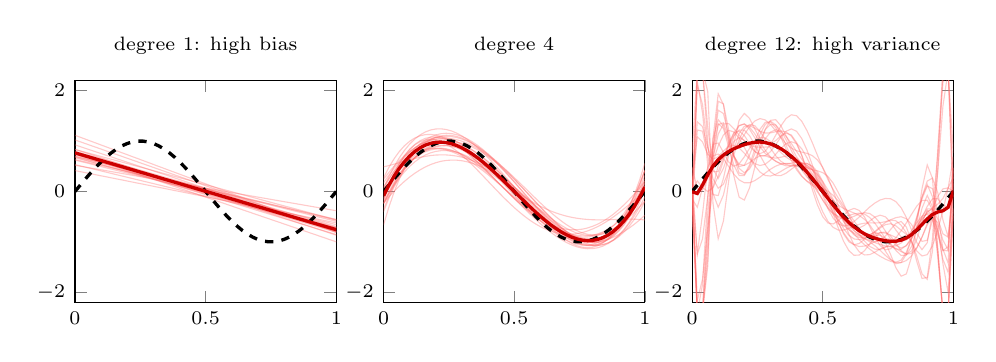
\begin{tikzpicture}
      \begin{groupplot}[group style={group size=3 by 1, horizontal sep=0.6cm}, width=4.9cm, height=4.4cm,
          xmin=0, xmax=1, ymin=-2.2, ymax=2.2, xtick={0,0.5,1}, ytick={-2,0,2}, tick label style={font=\scriptsize}, title style={font=\scriptsize},
          yticklabel style={font=\scriptsize}]
        \nextgroupplot[title={degree 1: high bias}]
\addplot[red!60, opacity=0.35, forget plot] coordinates {(0.000,0.727) (0.020,0.696) (0.040,0.664) (0.060,0.632) (0.080,0.601) (0.100,0.569) (0.120,0.537) (0.140,0.506) (0.160,0.474) (0.180,0.443) (0.200,0.411) (0.220,0.379) (0.240,0.348) (0.260,0.316) (0.280,0.284) (0.300,0.253) (0.320,0.221) (0.340,0.190) (0.360,0.158) (0.380,0.126) (0.400,0.095) (0.420,0.063) (0.440,0.031) (0.460,-0.000) (0.480,-0.032) (0.500,-0.063) (0.520,-0.095) (0.540,-0.127) (0.560,-0.158) (0.580,-0.190) (0.600,-0.222) (0.620,-0.253) (0.640,-0.285) (0.660,-0.316) (0.680,-0.348) (0.700,-0.380) (0.720,-0.411) (0.740,-0.443) (0.760,-0.475) (0.780,-0.506) (0.800,-0.538) (0.820,-0.569) (0.840,-0.601) (0.860,-0.633) (0.880,-0.664) (0.900,-0.696) (0.920,-0.728) (0.940,-0.759) (0.960,-0.791) (0.980,-0.822) (1.000,-0.854)};
\addplot[red!60, opacity=0.35, forget plot] coordinates {(0.000,1.021) (0.020,0.985) (0.040,0.949) (0.060,0.912) (0.080,0.876) (0.100,0.840) (0.120,0.803) (0.140,0.767) (0.160,0.731) (0.180,0.695) (0.200,0.658) (0.220,0.622) (0.240,0.586) (0.260,0.549) (0.280,0.513) (0.300,0.477) (0.320,0.440) (0.340,0.404) (0.360,0.368) (0.380,0.331) (0.400,0.295) (0.420,0.259) (0.440,0.222) (0.460,0.186) (0.480,0.150) (0.500,0.113) (0.520,0.077) (0.540,0.041) (0.560,0.005) (0.580,-0.032) (0.600,-0.068) (0.620,-0.104) (0.640,-0.141) (0.660,-0.177) (0.680,-0.213) (0.700,-0.250) (0.720,-0.286) (0.740,-0.322) (0.760,-0.359) (0.780,-0.395) (0.800,-0.431) (0.820,-0.468) (0.840,-0.504) (0.860,-0.540) (0.880,-0.577) (0.900,-0.613) (0.920,-0.649) (0.940,-0.686) (0.960,-0.722) (0.980,-0.758) (1.000,-0.794)};
\addplot[red!60, opacity=0.35, forget plot] coordinates {(0.000,0.622) (0.020,0.596) (0.040,0.571) (0.060,0.545) (0.080,0.519) (0.100,0.494) (0.120,0.468) (0.140,0.443) (0.160,0.417) (0.180,0.391) (0.200,0.366) (0.220,0.340) (0.240,0.315) (0.260,0.289) (0.280,0.263) (0.300,0.238) (0.320,0.212) (0.340,0.187) (0.360,0.161) (0.380,0.135) (0.400,0.110) (0.420,0.084) (0.440,0.059) (0.460,0.033) (0.480,0.007) (0.500,-0.018) (0.520,-0.044) (0.540,-0.069) (0.560,-0.095) (0.580,-0.121) (0.600,-0.146) (0.620,-0.172) (0.640,-0.198) (0.660,-0.223) (0.680,-0.249) (0.700,-0.274) (0.720,-0.300) (0.740,-0.326) (0.760,-0.351) (0.780,-0.377) (0.800,-0.402) (0.820,-0.428) (0.840,-0.454) (0.860,-0.479) (0.880,-0.505) (0.900,-0.530) (0.920,-0.556) (0.940,-0.582) (0.960,-0.607) (0.980,-0.633) (1.000,-0.658)};
\addplot[red!60, opacity=0.35, forget plot] coordinates {(0.000,0.775) (0.020,0.739) (0.040,0.704) (0.060,0.668) (0.080,0.633) (0.100,0.597) (0.120,0.562) (0.140,0.526) (0.160,0.491) (0.180,0.455) (0.200,0.420) (0.220,0.384) (0.240,0.349) (0.260,0.313) (0.280,0.278) (0.300,0.242) (0.320,0.207) (0.340,0.171) (0.360,0.136) (0.380,0.101) (0.400,0.065) (0.420,0.030) (0.440,-0.006) (0.460,-0.041) (0.480,-0.077) (0.500,-0.112) (0.520,-0.148) (0.540,-0.183) (0.560,-0.219) (0.580,-0.254) (0.600,-0.290) (0.620,-0.325) (0.640,-0.361) (0.660,-0.396) (0.680,-0.432) (0.700,-0.467) (0.720,-0.503) (0.740,-0.538) (0.760,-0.574) (0.780,-0.609) (0.800,-0.644) (0.820,-0.680) (0.840,-0.715) (0.860,-0.751) (0.880,-0.786) (0.900,-0.822) (0.920,-0.857) (0.940,-0.893) (0.960,-0.928) (0.980,-0.964) (1.000,-0.999)};
\addplot[red!60, opacity=0.35, forget plot] coordinates {(0.000,0.414) (0.020,0.393) (0.040,0.373) (0.060,0.352) (0.080,0.331) (0.100,0.310) (0.120,0.290) (0.140,0.269) (0.160,0.248) (0.180,0.228) (0.200,0.207) (0.220,0.186) (0.240,0.165) (0.260,0.145) (0.280,0.124) (0.300,0.103) (0.320,0.082) (0.340,0.062) (0.360,0.041) (0.380,0.020) (0.400,-0.000) (0.420,-0.021) (0.440,-0.042) (0.460,-0.063) (0.480,-0.083) (0.500,-0.104) (0.520,-0.125) (0.540,-0.146) (0.560,-0.166) (0.580,-0.187) (0.600,-0.208) (0.620,-0.228) (0.640,-0.249) (0.660,-0.270) (0.680,-0.291) (0.700,-0.311) (0.720,-0.332) (0.740,-0.353) (0.760,-0.374) (0.780,-0.394) (0.800,-0.415) (0.820,-0.436) (0.840,-0.456) (0.860,-0.477) (0.880,-0.498) (0.900,-0.519) (0.920,-0.539) (0.940,-0.560) (0.960,-0.581) (0.980,-0.602) (1.000,-0.622)};
\addplot[red!60, opacity=0.35, forget plot] coordinates {(0.000,0.532) (0.020,0.507) (0.040,0.482) (0.060,0.457) (0.080,0.432) (0.100,0.407) (0.120,0.382) (0.140,0.357) (0.160,0.331) (0.180,0.306) (0.200,0.281) (0.220,0.256) (0.240,0.231) (0.260,0.206) (0.280,0.181) (0.300,0.156) (0.320,0.131) (0.340,0.106) (0.360,0.081) (0.380,0.056) (0.400,0.031) (0.420,0.005) (0.440,-0.020) (0.460,-0.045) (0.480,-0.070) (0.500,-0.095) (0.520,-0.120) (0.540,-0.145) (0.560,-0.170) (0.580,-0.195) (0.600,-0.220) (0.620,-0.245) (0.640,-0.270) (0.660,-0.296) (0.680,-0.321) (0.700,-0.346) (0.720,-0.371) (0.740,-0.396) (0.760,-0.421) (0.780,-0.446) (0.800,-0.471) (0.820,-0.496) (0.840,-0.521) (0.860,-0.546) (0.880,-0.571) (0.900,-0.596) (0.920,-0.622) (0.940,-0.647) (0.960,-0.672) (0.980,-0.697) (1.000,-0.722)};
\addplot[red!60, opacity=0.35, forget plot] coordinates {(0.000,0.765) (0.020,0.735) (0.040,0.706) (0.060,0.676) (0.080,0.647) (0.100,0.617) (0.120,0.588) (0.140,0.558) (0.160,0.529) (0.180,0.499) (0.200,0.469) (0.220,0.440) (0.240,0.410) (0.260,0.381) (0.280,0.351) (0.300,0.322) (0.320,0.292) (0.340,0.263) (0.360,0.233) (0.380,0.204) (0.400,0.174) (0.420,0.144) (0.440,0.115) (0.460,0.085) (0.480,0.056) (0.500,0.026) (0.520,-0.003) (0.540,-0.033) (0.560,-0.062) (0.580,-0.092) (0.600,-0.121) (0.620,-0.151) (0.640,-0.180) (0.660,-0.210) (0.680,-0.240) (0.700,-0.269) (0.720,-0.299) (0.740,-0.328) (0.760,-0.358) (0.780,-0.387) (0.800,-0.417) (0.820,-0.446) (0.840,-0.476) (0.860,-0.505) (0.880,-0.535) (0.900,-0.565) (0.920,-0.594) (0.940,-0.624) (0.960,-0.653) (0.980,-0.683) (1.000,-0.712)};
\addplot[red!60, opacity=0.35, forget plot] coordinates {(0.000,0.832) (0.020,0.804) (0.040,0.776) (0.060,0.749) (0.080,0.721) (0.100,0.693) (0.120,0.665) (0.140,0.637) (0.160,0.609) (0.180,0.581) (0.200,0.553) (0.220,0.525) (0.240,0.497) (0.260,0.469) (0.280,0.441) (0.300,0.413) (0.320,0.385) (0.340,0.357) (0.360,0.329) (0.380,0.301) (0.400,0.273) (0.420,0.245) (0.440,0.218) (0.460,0.190) (0.480,0.162) (0.500,0.134) (0.520,0.106) (0.540,0.078) (0.560,0.050) (0.580,0.022) (0.600,-0.006) (0.620,-0.034) (0.640,-0.062) (0.660,-0.090) (0.680,-0.118) (0.700,-0.146) (0.720,-0.174) (0.740,-0.202) (0.760,-0.230) (0.780,-0.258) (0.800,-0.286) (0.820,-0.313) (0.840,-0.341) (0.860,-0.369) (0.880,-0.397) (0.900,-0.425) (0.920,-0.453) (0.940,-0.481) (0.960,-0.509) (0.980,-0.537) (1.000,-0.565)};
\addplot[red!60, opacity=0.35, forget plot] coordinates {(0.000,0.669) (0.020,0.641) (0.040,0.613) (0.060,0.585) (0.080,0.557) (0.100,0.530) (0.120,0.502) (0.140,0.474) (0.160,0.446) (0.180,0.418) (0.200,0.391) (0.220,0.363) (0.240,0.335) (0.260,0.307) (0.280,0.279) (0.300,0.252) (0.320,0.224) (0.340,0.196) (0.360,0.168) (0.380,0.140) (0.400,0.113) (0.420,0.085) (0.440,0.057) (0.460,0.029) (0.480,0.001) (0.500,-0.026) (0.520,-0.054) (0.540,-0.082) (0.560,-0.110) (0.580,-0.138) (0.600,-0.165) (0.620,-0.193) (0.640,-0.221) (0.660,-0.249) (0.680,-0.277) (0.700,-0.304) (0.720,-0.332) (0.740,-0.360) (0.760,-0.388) (0.780,-0.416) (0.800,-0.443) (0.820,-0.471) (0.840,-0.499) (0.860,-0.527) (0.880,-0.555) (0.900,-0.582) (0.920,-0.610) (0.940,-0.638) (0.960,-0.666) (0.980,-0.694) (1.000,-0.721)};
\addplot[red!60, opacity=0.35, forget plot] coordinates {(0.000,0.768) (0.020,0.736) (0.040,0.705) (0.060,0.674) (0.080,0.643) (0.100,0.611) (0.120,0.580) (0.140,0.549) (0.160,0.518) (0.180,0.487) (0.200,0.455) (0.220,0.424) (0.240,0.393) (0.260,0.362) (0.280,0.331) (0.300,0.299) (0.320,0.268) (0.340,0.237) (0.360,0.206) (0.380,0.174) (0.400,0.143) (0.420,0.112) (0.440,0.081) (0.460,0.050) (0.480,0.018) (0.500,-0.013) (0.520,-0.044) (0.540,-0.075) (0.560,-0.107) (0.580,-0.138) (0.600,-0.169) (0.620,-0.200) (0.640,-0.231) (0.660,-0.263) (0.680,-0.294) (0.700,-0.325) (0.720,-0.356) (0.740,-0.388) (0.760,-0.419) (0.780,-0.450) (0.800,-0.481) (0.820,-0.512) (0.840,-0.544) (0.860,-0.575) (0.880,-0.606) (0.900,-0.637) (0.920,-0.669) (0.940,-0.700) (0.960,-0.731) (0.980,-0.762) (1.000,-0.793)};
\addplot[red!60, opacity=0.35, forget plot] coordinates {(0.000,0.738) (0.020,0.707) (0.040,0.676) (0.060,0.645) (0.080,0.614) (0.100,0.583) (0.120,0.552) (0.140,0.521) (0.160,0.490) (0.180,0.459) (0.200,0.428) (0.220,0.397) (0.240,0.366) (0.260,0.335) (0.280,0.305) (0.300,0.274) (0.320,0.243) (0.340,0.212) (0.360,0.181) (0.380,0.150) (0.400,0.119) (0.420,0.088) (0.440,0.057) (0.460,0.026) (0.480,-0.005) (0.500,-0.036) (0.520,-0.067) (0.540,-0.098) (0.560,-0.129) (0.580,-0.160) (0.600,-0.191) (0.620,-0.222) (0.640,-0.253) (0.660,-0.284) (0.680,-0.315) (0.700,-0.346) (0.720,-0.377) (0.740,-0.408) (0.760,-0.439) (0.780,-0.470) (0.800,-0.501) (0.820,-0.532) (0.840,-0.562) (0.860,-0.593) (0.880,-0.624) (0.900,-0.655) (0.920,-0.686) (0.940,-0.717) (0.960,-0.748) (0.980,-0.779) (1.000,-0.810)};
\addplot[red!60, opacity=0.35, forget plot] coordinates {(0.000,0.696) (0.020,0.671) (0.040,0.645) (0.060,0.619) (0.080,0.593) (0.100,0.567) (0.120,0.542) (0.140,0.516) (0.160,0.490) (0.180,0.464) (0.200,0.438) (0.220,0.413) (0.240,0.387) (0.260,0.361) (0.280,0.335) (0.300,0.309) (0.320,0.284) (0.340,0.258) (0.360,0.232) (0.380,0.206) (0.400,0.180) (0.420,0.154) (0.440,0.129) (0.460,0.103) (0.480,0.077) (0.500,0.051) (0.520,0.025) (0.540,-0.000) (0.560,-0.026) (0.580,-0.052) (0.600,-0.078) (0.620,-0.104) (0.640,-0.129) (0.660,-0.155) (0.680,-0.181) (0.700,-0.207) (0.720,-0.233) (0.740,-0.258) (0.760,-0.284) (0.780,-0.310) (0.800,-0.336) (0.820,-0.362) (0.840,-0.387) (0.860,-0.413) (0.880,-0.439) (0.900,-0.465) (0.920,-0.491) (0.940,-0.516) (0.960,-0.542) (0.980,-0.568) (1.000,-0.594)};
\addplot[red!60, opacity=0.35, forget plot] coordinates {(0.000,0.684) (0.020,0.655) (0.040,0.625) (0.060,0.596) (0.080,0.567) (0.100,0.538) (0.120,0.508) (0.140,0.479) (0.160,0.450) (0.180,0.420) (0.200,0.391) (0.220,0.362) (0.240,0.332) (0.260,0.303) (0.280,0.274) (0.300,0.244) (0.320,0.215) (0.340,0.186) (0.360,0.156) (0.380,0.127) (0.400,0.098) (0.420,0.068) (0.440,0.039) (0.460,0.010) (0.480,-0.020) (0.500,-0.049) (0.520,-0.078) (0.540,-0.107) (0.560,-0.137) (0.580,-0.166) (0.600,-0.195) (0.620,-0.225) (0.640,-0.254) (0.660,-0.283) (0.680,-0.313) (0.700,-0.342) (0.720,-0.371) (0.740,-0.401) (0.760,-0.430) (0.780,-0.459) (0.800,-0.489) (0.820,-0.518) (0.840,-0.547) (0.860,-0.577) (0.880,-0.606) (0.900,-0.635) (0.920,-0.664) (0.940,-0.694) (0.960,-0.723) (0.980,-0.752) (1.000,-0.782)};
\addplot[red!60, opacity=0.35, forget plot] coordinates {(0.000,0.923) (0.020,0.889) (0.040,0.854) (0.060,0.820) (0.080,0.786) (0.100,0.751) (0.120,0.717) (0.140,0.683) (0.160,0.648) (0.180,0.614) (0.200,0.579) (0.220,0.545) (0.240,0.511) (0.260,0.476) (0.280,0.442) (0.300,0.408) (0.320,0.373) (0.340,0.339) (0.360,0.305) (0.380,0.270) (0.400,0.236) (0.420,0.201) (0.440,0.167) (0.460,0.133) (0.480,0.098) (0.500,0.064) (0.520,0.030) (0.540,-0.005) (0.560,-0.039) (0.580,-0.074) (0.600,-0.108) (0.620,-0.142) (0.640,-0.177) (0.660,-0.211) (0.680,-0.245) (0.700,-0.280) (0.720,-0.314) (0.740,-0.348) (0.760,-0.383) (0.780,-0.417) (0.800,-0.452) (0.820,-0.486) (0.840,-0.520) (0.860,-0.555) (0.880,-0.589) (0.900,-0.623) (0.920,-0.658) (0.940,-0.692) (0.960,-0.727) (0.980,-0.761) (1.000,-0.795)};
\addplot[red!60, opacity=0.35, forget plot] coordinates {(0.000,0.697) (0.020,0.672) (0.040,0.647) (0.060,0.621) (0.080,0.596) (0.100,0.571) (0.120,0.545) (0.140,0.520) (0.160,0.494) (0.180,0.469) (0.200,0.444) (0.220,0.418) (0.240,0.393) (0.260,0.368) (0.280,0.342) (0.300,0.317) (0.320,0.292) (0.340,0.266) (0.360,0.241) (0.380,0.215) (0.400,0.190) (0.420,0.165) (0.440,0.139) (0.460,0.114) (0.480,0.089) (0.500,0.063) (0.520,0.038) (0.540,0.013) (0.560,-0.013) (0.580,-0.038) (0.600,-0.064) (0.620,-0.089) (0.640,-0.114) (0.660,-0.140) (0.680,-0.165) (0.700,-0.190) (0.720,-0.216) (0.740,-0.241) (0.760,-0.267) (0.780,-0.292) (0.800,-0.317) (0.820,-0.343) (0.840,-0.368) (0.860,-0.393) (0.880,-0.419) (0.900,-0.444) (0.920,-0.469) (0.940,-0.495) (0.960,-0.520) (0.980,-0.546) (1.000,-0.571)};
\addplot[red!60, opacity=0.35, forget plot] coordinates {(0.000,0.519) (0.020,0.501) (0.040,0.483) (0.060,0.465) (0.080,0.447) (0.100,0.429) (0.120,0.411) (0.140,0.393) (0.160,0.375) (0.180,0.357) (0.200,0.339) (0.220,0.320) (0.240,0.302) (0.260,0.284) (0.280,0.266) (0.300,0.248) (0.320,0.230) (0.340,0.212) (0.360,0.194) (0.380,0.176) (0.400,0.158) (0.420,0.140) (0.440,0.122) (0.460,0.104) (0.480,0.086) (0.500,0.068) (0.520,0.050) (0.540,0.032) (0.560,0.014) (0.580,-0.004) (0.600,-0.022) (0.620,-0.040) (0.640,-0.058) (0.660,-0.076) (0.680,-0.094) (0.700,-0.112) (0.720,-0.130) (0.740,-0.148) (0.760,-0.166) (0.780,-0.184) (0.800,-0.202) (0.820,-0.220) (0.840,-0.238) (0.860,-0.256) (0.880,-0.274) (0.900,-0.292) (0.920,-0.310) (0.940,-0.328) (0.960,-0.346) (0.980,-0.364) (1.000,-0.382)};
\addplot[red!60, opacity=0.35, forget plot] coordinates {(0.000,0.797) (0.020,0.767) (0.040,0.737) (0.060,0.708) (0.080,0.678) (0.100,0.648) (0.120,0.618) (0.140,0.588) (0.160,0.558) (0.180,0.529) (0.200,0.499) (0.220,0.469) (0.240,0.439) (0.260,0.409) (0.280,0.379) (0.300,0.349) (0.320,0.320) (0.340,0.290) (0.360,0.260) (0.380,0.230) (0.400,0.200) (0.420,0.170) (0.440,0.141) (0.460,0.111) (0.480,0.081) (0.500,0.051) (0.520,0.021) (0.540,-0.009) (0.560,-0.039) (0.580,-0.068) (0.600,-0.098) (0.620,-0.128) (0.640,-0.158) (0.660,-0.188) (0.680,-0.218) (0.700,-0.248) (0.720,-0.277) (0.740,-0.307) (0.760,-0.337) (0.780,-0.367) (0.800,-0.397) (0.820,-0.427) (0.840,-0.456) (0.860,-0.486) (0.880,-0.516) (0.900,-0.546) (0.920,-0.576) (0.940,-0.606) (0.960,-0.636) (0.980,-0.665) (1.000,-0.695)};
\addplot[red!60, opacity=0.35, forget plot] coordinates {(0.000,1.114) (0.020,1.075) (0.040,1.037) (0.060,0.998) (0.080,0.960) (0.100,0.921) (0.120,0.883) (0.140,0.844) (0.160,0.806) (0.180,0.767) (0.200,0.729) (0.220,0.690) (0.240,0.652) (0.260,0.613) (0.280,0.575) (0.300,0.536) (0.320,0.497) (0.340,0.459) (0.360,0.420) (0.380,0.382) (0.400,0.343) (0.420,0.305) (0.440,0.266) (0.460,0.228) (0.480,0.189) (0.500,0.151) (0.520,0.112) (0.540,0.074) (0.560,0.035) (0.580,-0.003) (0.600,-0.042) (0.620,-0.081) (0.640,-0.119) (0.660,-0.158) (0.680,-0.196) (0.700,-0.235) (0.720,-0.273) (0.740,-0.312) (0.760,-0.350) (0.780,-0.389) (0.800,-0.427) (0.820,-0.466) (0.840,-0.504) (0.860,-0.543) (0.880,-0.581) (0.900,-0.620) (0.920,-0.659) (0.940,-0.697) (0.960,-0.736) (0.980,-0.774) (1.000,-0.813)};
\addplot[red!60, opacity=0.35, forget plot] coordinates {(0.000,0.633) (0.020,0.610) (0.040,0.586) (0.060,0.562) (0.080,0.538) (0.100,0.515) (0.120,0.491) (0.140,0.467) (0.160,0.443) (0.180,0.420) (0.200,0.396) (0.220,0.372) (0.240,0.348) (0.260,0.325) (0.280,0.301) (0.300,0.277) (0.320,0.253) (0.340,0.230) (0.360,0.206) (0.380,0.182) (0.400,0.158) (0.420,0.135) (0.440,0.111) (0.460,0.087) (0.480,0.063) (0.500,0.040) (0.520,0.016) (0.540,-0.008) (0.560,-0.031) (0.580,-0.055) (0.600,-0.079) (0.620,-0.103) (0.640,-0.126) (0.660,-0.150) (0.680,-0.174) (0.700,-0.198) (0.720,-0.221) (0.740,-0.245) (0.760,-0.269) (0.780,-0.293) (0.800,-0.316) (0.820,-0.340) (0.840,-0.364) (0.860,-0.388) (0.880,-0.411) (0.900,-0.435) (0.920,-0.459) (0.940,-0.483) (0.960,-0.506) (0.980,-0.530) (1.000,-0.554)};
\addplot[red!60, opacity=0.35, forget plot] coordinates {(0.000,0.836) (0.020,0.802) (0.040,0.768) (0.060,0.734) (0.080,0.700) (0.100,0.666) (0.120,0.632) (0.140,0.598) (0.160,0.564) (0.180,0.530) (0.200,0.495) (0.220,0.461) (0.240,0.427) (0.260,0.393) (0.280,0.359) (0.300,0.325) (0.320,0.291) (0.340,0.257) (0.360,0.223) (0.380,0.189) (0.400,0.155) (0.420,0.121) (0.440,0.087) (0.460,0.053) (0.480,0.018) (0.500,-0.016) (0.520,-0.050) (0.540,-0.084) (0.560,-0.118) (0.580,-0.152) (0.600,-0.186) (0.620,-0.220) (0.640,-0.254) (0.660,-0.288) (0.680,-0.322) (0.700,-0.356) (0.720,-0.390) (0.740,-0.424) (0.760,-0.459) (0.780,-0.493) (0.800,-0.527) (0.820,-0.561) (0.840,-0.595) (0.860,-0.629) (0.880,-0.663) (0.900,-0.697) (0.920,-0.731) (0.940,-0.765) (0.960,-0.799) (0.980,-0.833) (1.000,-0.867)};
\addplot[black, very thick, dashed] coordinates {(0.000,0.000) (0.020,0.125) (0.040,0.249) (0.060,0.368) (0.080,0.482) (0.100,0.588) (0.120,0.685) (0.140,0.771) (0.160,0.844) (0.180,0.905) (0.200,0.951) (0.220,0.982) (0.240,0.998) (0.260,0.998) (0.280,0.982) (0.300,0.951) (0.320,0.905) (0.340,0.844) (0.360,0.771) (0.380,0.685) (0.400,0.588) (0.420,0.482) (0.440,0.368) (0.460,0.249) (0.480,0.125) (0.500,0.000) (0.520,-0.125) (0.540,-0.249) (0.560,-0.368) (0.580,-0.482) (0.600,-0.588) (0.620,-0.685) (0.640,-0.771) (0.660,-0.844) (0.680,-0.905) (0.700,-0.951) (0.720,-0.982) (0.740,-0.998) (0.760,-0.998) (0.780,-0.982) (0.800,-0.951) (0.820,-0.905) (0.840,-0.844) (0.860,-0.771) (0.880,-0.685) (0.900,-0.588) (0.920,-0.482) (0.940,-0.368) (0.960,-0.249) (0.980,-0.125) (1.000,-0.000)};
\addplot[red!80!black, very thick] coordinates {(0.000,0.765) (0.020,0.735) (0.040,0.704) (0.060,0.674) (0.080,0.643) (0.100,0.613) (0.120,0.582) (0.140,0.552) (0.160,0.521) (0.180,0.491) (0.200,0.460) (0.220,0.430) (0.240,0.399) (0.260,0.369) (0.280,0.339) (0.300,0.308) (0.320,0.278) (0.340,0.247) (0.360,0.217) (0.380,0.186) (0.400,0.156) (0.420,0.125) (0.440,0.095) (0.460,0.064) (0.480,0.034) (0.500,0.004) (0.520,-0.027) (0.540,-0.057) (0.560,-0.088) (0.580,-0.118) (0.600,-0.149) (0.620,-0.179) (0.640,-0.210) (0.660,-0.240) (0.680,-0.271) (0.700,-0.301) (0.720,-0.331) (0.740,-0.362) (0.760,-0.392) (0.780,-0.423) (0.800,-0.453) (0.820,-0.484) (0.840,-0.514) (0.860,-0.545) (0.880,-0.575) (0.900,-0.606) (0.920,-0.636) (0.940,-0.667) (0.960,-0.697) (0.980,-0.727) (1.000,-0.758)};
        \nextgroupplot[title={degree 4}]
\addplot[red!60, opacity=0.35, forget plot] coordinates {(0.000,-0.163) (0.020,0.120) (0.040,0.359) (0.060,0.556) (0.080,0.714) (0.100,0.837) (0.120,0.927) (0.140,0.988) (0.160,1.022) (0.180,1.032) (0.200,1.020) (0.220,0.989) (0.240,0.941) (0.260,0.878) (0.280,0.803) (0.300,0.718) (0.320,0.624) (0.340,0.524) (0.360,0.419) (0.380,0.312) (0.400,0.202) (0.420,0.093) (0.440,-0.015) (0.460,-0.121) (0.480,-0.222) (0.500,-0.319) (0.520,-0.409) (0.540,-0.493) (0.560,-0.570) (0.580,-0.638) (0.600,-0.697) (0.620,-0.747) (0.640,-0.787) (0.660,-0.817) (0.680,-0.837) (0.700,-0.847) (0.720,-0.846) (0.740,-0.836) (0.760,-0.815) (0.780,-0.784) (0.800,-0.744) (0.820,-0.696) (0.840,-0.639) (0.860,-0.575) (0.880,-0.503) (0.900,-0.427) (0.920,-0.345) (0.940,-0.259) (0.960,-0.171) (0.980,-0.082) (1.000,0.008)};
\addplot[red!60, opacity=0.35, forget plot] coordinates {(0.000,0.058) (0.020,0.288) (0.040,0.490) (0.060,0.665) (0.080,0.814) (0.100,0.940) (0.120,1.041) (0.140,1.121) (0.160,1.180) (0.180,1.219) (0.200,1.239) (0.220,1.242) (0.240,1.228) (0.260,1.200) (0.280,1.157) (0.300,1.101) (0.320,1.034) (0.340,0.956) (0.360,0.868) (0.380,0.773) (0.400,0.670) (0.420,0.561) (0.440,0.448) (0.460,0.331) (0.480,0.212) (0.500,0.092) (0.520,-0.029) (0.540,-0.148) (0.560,-0.265) (0.580,-0.379) (0.600,-0.488) (0.620,-0.592) (0.640,-0.688) (0.660,-0.776) (0.680,-0.855) (0.700,-0.923) (0.720,-0.980) (0.740,-1.024) (0.760,-1.054) (0.780,-1.069) (0.800,-1.067) (0.820,-1.048) (0.840,-1.010) (0.860,-0.952) (0.880,-0.873) (0.900,-0.772) (0.920,-0.647) (0.940,-0.498) (0.960,-0.323) (0.980,-0.121) (1.000,0.110)};
\addplot[red!60, opacity=0.35, forget plot] coordinates {(0.000,-0.664) (0.020,-0.318) (0.040,-0.017) (0.060,0.240) (0.080,0.458) (0.100,0.638) (0.120,0.783) (0.140,0.897) (0.160,0.980) (0.180,1.037) (0.200,1.069) (0.220,1.078) (0.240,1.066) (0.260,1.037) (0.280,0.991) (0.300,0.931) (0.320,0.858) (0.340,0.775) (0.360,0.683) (0.380,0.584) (0.400,0.480) (0.420,0.371) (0.440,0.259) (0.460,0.147) (0.480,0.034) (0.500,-0.077) (0.520,-0.187) (0.540,-0.292) (0.560,-0.394) (0.580,-0.489) (0.600,-0.579) (0.620,-0.662) (0.640,-0.738) (0.660,-0.805) (0.680,-0.863) (0.700,-0.913) (0.720,-0.952) (0.740,-0.982) (0.760,-1.002) (0.780,-1.012) (0.800,-1.011) (0.820,-1.000) (0.840,-0.979) (0.860,-0.947) (0.880,-0.906) (0.900,-0.855) (0.920,-0.795) (0.940,-0.726) (0.960,-0.650) (0.980,-0.565) (1.000,-0.473)};
\addplot[red!60, opacity=0.35, forget plot] coordinates {(0.000,0.488) (0.020,0.513) (0.040,0.541) (0.060,0.570) (0.080,0.599) (0.100,0.627) (0.120,0.654) (0.140,0.677) (0.160,0.696) (0.180,0.712) (0.200,0.722) (0.220,0.726) (0.240,0.724) (0.260,0.716) (0.280,0.701) (0.300,0.679) (0.320,0.650) (0.340,0.614) (0.360,0.570) (0.380,0.520) (0.400,0.463) (0.420,0.399) (0.440,0.329) (0.460,0.254) (0.480,0.174) (0.500,0.089) (0.520,0.000) (0.540,-0.091) (0.560,-0.185) (0.580,-0.279) (0.600,-0.374) (0.620,-0.467) (0.640,-0.558) (0.660,-0.645) (0.680,-0.726) (0.700,-0.801) (0.720,-0.868) (0.740,-0.925) (0.760,-0.970) (0.780,-1.001) (0.800,-1.017) (0.820,-1.015) (0.840,-0.994) (0.860,-0.951) (0.880,-0.884) (0.900,-0.790) (0.920,-0.667) (0.940,-0.513) (0.960,-0.326) (0.980,-0.101) (1.000,0.163)};
\addplot[red!60, opacity=0.35, forget plot] coordinates {(0.000,-0.403) (0.020,-0.140) (0.040,0.085) (0.060,0.277) (0.080,0.437) (0.100,0.567) (0.120,0.671) (0.140,0.749) (0.160,0.806) (0.180,0.841) (0.200,0.859) (0.220,0.859) (0.240,0.845) (0.260,0.819) (0.280,0.780) (0.300,0.733) (0.320,0.677) (0.340,0.615) (0.360,0.547) (0.380,0.476) (0.400,0.401) (0.420,0.325) (0.440,0.248) (0.460,0.172) (0.480,0.097) (0.500,0.023) (0.520,-0.047) (0.540,-0.115) (0.560,-0.178) (0.580,-0.238) (0.600,-0.292) (0.620,-0.342) (0.640,-0.387) (0.660,-0.426) (0.680,-0.460) (0.700,-0.489) (0.720,-0.513) (0.740,-0.531) (0.760,-0.545) (0.780,-0.555) (0.800,-0.561) (0.820,-0.563) (0.840,-0.563) (0.860,-0.561) (0.880,-0.558) (0.900,-0.554) (0.920,-0.551) (0.940,-0.549) (0.960,-0.550) (0.980,-0.555) (1.000,-0.565)};
\addplot[red!60, opacity=0.35, forget plot] coordinates {(0.000,-0.123) (0.020,0.053) (0.040,0.212) (0.060,0.353) (0.080,0.478) (0.100,0.585) (0.120,0.676) (0.140,0.751) (0.160,0.811) (0.180,0.856) (0.200,0.887) (0.220,0.904) (0.240,0.908) (0.260,0.900) (0.280,0.880) (0.300,0.848) (0.320,0.807) (0.340,0.756) (0.360,0.695) (0.380,0.627) (0.400,0.552) (0.420,0.470) (0.440,0.383) (0.460,0.291) (0.480,0.196) (0.500,0.097) (0.520,-0.002) (0.540,-0.103) (0.560,-0.203) (0.580,-0.301) (0.600,-0.397) (0.620,-0.489) (0.640,-0.576) (0.660,-0.657) (0.680,-0.730) (0.700,-0.795) (0.720,-0.850) (0.740,-0.894) (0.760,-0.925) (0.780,-0.943) (0.800,-0.945) (0.820,-0.930) (0.840,-0.897) (0.860,-0.845) (0.880,-0.772) (0.900,-0.675) (0.920,-0.555) (0.940,-0.408) (0.960,-0.235) (0.980,-0.032) (1.000,0.202)};
\addplot[red!60, opacity=0.35, forget plot] coordinates {(0.000,0.091) (0.020,0.254) (0.040,0.396) (0.060,0.516) (0.080,0.616) (0.100,0.697) (0.120,0.761) (0.140,0.807) (0.160,0.838) (0.180,0.854) (0.200,0.856) (0.220,0.845) (0.240,0.823) (0.260,0.789) (0.280,0.746) (0.300,0.694) (0.320,0.633) (0.340,0.566) (0.360,0.493) (0.380,0.414) (0.400,0.332) (0.420,0.246) (0.440,0.157) (0.460,0.067) (0.480,-0.023) (0.500,-0.114) (0.520,-0.203) (0.540,-0.290) (0.560,-0.375) (0.580,-0.455) (0.600,-0.531) (0.620,-0.602) (0.640,-0.667) (0.660,-0.725) (0.680,-0.775) (0.700,-0.816) (0.720,-0.848) (0.740,-0.870) (0.760,-0.881) (0.780,-0.880) (0.800,-0.867) (0.820,-0.841) (0.840,-0.801) (0.860,-0.746) (0.880,-0.676) (0.900,-0.589) (0.920,-0.486) (0.940,-0.366) (0.960,-0.227) (0.980,-0.069) (1.000,0.108)};
\addplot[red!60, opacity=0.35, forget plot] coordinates {(0.000,-0.349) (0.020,-0.102) (0.040,0.120) (0.060,0.317) (0.080,0.490) (0.100,0.640) (0.120,0.767) (0.140,0.874) (0.160,0.959) (0.180,1.025) (0.200,1.073) (0.220,1.102) (0.240,1.114) (0.260,1.110) (0.280,1.091) (0.300,1.058) (0.320,1.012) (0.340,0.954) (0.360,0.885) (0.380,0.806) (0.400,0.718) (0.420,0.623) (0.440,0.521) (0.460,0.414) (0.480,0.302) (0.500,0.188) (0.520,0.072) (0.540,-0.045) (0.560,-0.161) (0.580,-0.275) (0.600,-0.385) (0.620,-0.491) (0.640,-0.591) (0.660,-0.683) (0.680,-0.767) (0.700,-0.840) (0.720,-0.902) (0.740,-0.950) (0.760,-0.984) (0.780,-1.002) (0.800,-1.002) (0.820,-0.983) (0.840,-0.943) (0.860,-0.881) (0.880,-0.795) (0.900,-0.683) (0.920,-0.544) (0.940,-0.377) (0.960,-0.178) (0.980,0.052) (1.000,0.317)};
\addplot[red!60, opacity=0.35, forget plot] coordinates {(0.000,-0.186) (0.020,0.095) (0.040,0.334) (0.060,0.534) (0.080,0.699) (0.100,0.831) (0.120,0.933) (0.140,1.006) (0.160,1.053) (0.180,1.077) (0.200,1.080) (0.220,1.064) (0.240,1.031) (0.260,0.982) (0.280,0.921) (0.300,0.849) (0.320,0.767) (0.340,0.677) (0.360,0.582) (0.380,0.481) (0.400,0.378) (0.420,0.274) (0.440,0.169) (0.460,0.064) (0.480,-0.037) (0.500,-0.136) (0.520,-0.230) (0.540,-0.319) (0.560,-0.402) (0.580,-0.478) (0.600,-0.546) (0.620,-0.606) (0.640,-0.656) (0.660,-0.698) (0.680,-0.729) (0.700,-0.750) (0.720,-0.760) (0.740,-0.759) (0.760,-0.748) (0.780,-0.725) (0.800,-0.691) (0.820,-0.647) (0.840,-0.591) (0.860,-0.525) (0.880,-0.449) (0.900,-0.362) (0.920,-0.267) (0.940,-0.162) (0.960,-0.049) (0.980,0.072) (1.000,0.200)};
\addplot[red!60, opacity=0.35, forget plot] coordinates {(0.000,-0.240) (0.020,-0.054) (0.040,0.113) (0.060,0.260) (0.080,0.388) (0.100,0.497) (0.120,0.589) (0.140,0.664) (0.160,0.723) (0.180,0.766) (0.200,0.794) (0.220,0.809) (0.240,0.810) (0.260,0.800) (0.280,0.777) (0.300,0.744) (0.320,0.700) (0.340,0.648) (0.360,0.587) (0.380,0.519) (0.400,0.445) (0.420,0.365) (0.440,0.280) (0.460,0.191) (0.480,0.099) (0.500,0.006) (0.520,-0.089) (0.540,-0.184) (0.560,-0.277) (0.580,-0.369) (0.600,-0.458) (0.620,-0.543) (0.640,-0.624) (0.660,-0.698) (0.680,-0.765) (0.700,-0.824) (0.720,-0.874) (0.740,-0.913) (0.760,-0.941) (0.780,-0.957) (0.800,-0.959) (0.820,-0.947) (0.840,-0.918) (0.860,-0.873) (0.880,-0.809) (0.900,-0.726) (0.920,-0.622) (0.940,-0.496) (0.960,-0.347) (0.980,-0.174) (1.000,0.024)};
\addplot[red!60, opacity=0.35, forget plot] coordinates {(0.000,0.266) (0.020,0.472) (0.040,0.646) (0.060,0.790) (0.080,0.906) (0.100,0.995) (0.120,1.061) (0.140,1.104) (0.160,1.127) (0.180,1.131) (0.200,1.117) (0.220,1.089) (0.240,1.046) (0.260,0.991) (0.280,0.925) (0.300,0.850) (0.320,0.767) (0.340,0.677) (0.360,0.582) (0.380,0.482) (0.400,0.380) (0.420,0.276) (0.440,0.171) (0.460,0.067) (0.480,-0.037) (0.500,-0.137) (0.520,-0.235) (0.540,-0.329) (0.560,-0.418) (0.580,-0.501) (0.600,-0.578) (0.620,-0.649) (0.640,-0.712) (0.660,-0.766) (0.680,-0.813) (0.700,-0.850) (0.720,-0.878) (0.740,-0.897) (0.760,-0.905) (0.780,-0.903) (0.800,-0.891) (0.820,-0.868) (0.840,-0.835) (0.860,-0.791) (0.880,-0.736) (0.900,-0.671) (0.920,-0.595) (0.940,-0.509) (0.960,-0.413) (0.980,-0.307) (1.000,-0.191)};
\addplot[red!60, opacity=0.35, forget plot] coordinates {(0.000,-0.240) (0.020,-0.044) (0.040,0.135) (0.060,0.295) (0.080,0.438) (0.100,0.563) (0.120,0.670) (0.140,0.760) (0.160,0.834) (0.180,0.890) (0.200,0.931) (0.220,0.957) (0.240,0.967) (0.260,0.963) (0.280,0.945) (0.300,0.914) (0.320,0.871) (0.340,0.816) (0.360,0.750) (0.380,0.674) (0.400,0.589) (0.420,0.497) (0.440,0.397) (0.460,0.292) (0.480,0.182) (0.500,0.068) (0.520,-0.048) (0.540,-0.165) (0.560,-0.282) (0.580,-0.397) (0.600,-0.509) (0.620,-0.616) (0.640,-0.718) (0.660,-0.811) (0.680,-0.895) (0.700,-0.969) (0.720,-1.029) (0.740,-1.075) (0.760,-1.104) (0.780,-1.115) (0.800,-1.106) (0.820,-1.075) (0.840,-1.020) (0.860,-0.938) (0.880,-0.828) (0.900,-0.687) (0.920,-0.514) (0.940,-0.305) (0.960,-0.059) (0.980,0.227) (1.000,0.555)};
\addplot[red!60, opacity=0.35, forget plot] coordinates {(0.000,0.239) (0.020,0.375) (0.040,0.498) (0.060,0.609) (0.080,0.707) (0.100,0.793) (0.120,0.867) (0.140,0.928) (0.160,0.977) (0.180,1.013) (0.200,1.039) (0.220,1.052) (0.240,1.054) (0.260,1.046) (0.280,1.026) (0.300,0.997) (0.320,0.958) (0.340,0.910) (0.360,0.854) (0.380,0.789) (0.400,0.718) (0.420,0.639) (0.440,0.555) (0.460,0.466) (0.480,0.373) (0.500,0.276) (0.520,0.176) (0.540,0.076) (0.560,-0.026) (0.580,-0.127) (0.600,-0.226) (0.620,-0.323) (0.640,-0.415) (0.660,-0.503) (0.680,-0.584) (0.700,-0.658) (0.720,-0.723) (0.740,-0.777) (0.760,-0.820) (0.780,-0.849) (0.800,-0.864) (0.820,-0.863) (0.840,-0.843) (0.860,-0.805) (0.880,-0.744) (0.900,-0.662) (0.920,-0.554) (0.940,-0.420) (0.960,-0.257) (0.980,-0.065) (1.000,0.160)};
\addplot[red!60, opacity=0.35, forget plot] coordinates {(0.000,0.025) (0.020,0.169) (0.040,0.302) (0.060,0.423) (0.080,0.534) (0.100,0.632) (0.120,0.719) (0.140,0.793) (0.160,0.856) (0.180,0.906) (0.200,0.943) (0.220,0.969) (0.240,0.983) (0.260,0.985) (0.280,0.975) (0.300,0.954) (0.320,0.922) (0.340,0.880) (0.360,0.828) (0.380,0.766) (0.400,0.696) (0.420,0.618) (0.440,0.533) (0.460,0.441) (0.480,0.343) (0.500,0.240) (0.520,0.134) (0.540,0.025) (0.560,-0.085) (0.580,-0.196) (0.600,-0.307) (0.620,-0.415) (0.640,-0.520) (0.660,-0.621) (0.680,-0.715) (0.700,-0.802) (0.720,-0.879) (0.740,-0.945) (0.760,-0.999) (0.780,-1.039) (0.800,-1.062) (0.820,-1.068) (0.840,-1.054) (0.860,-1.018) (0.880,-0.958) (0.900,-0.871) (0.920,-0.757) (0.940,-0.613) (0.960,-0.435) (0.980,-0.223) (1.000,0.027)};
\addplot[red!60, opacity=0.35, forget plot] coordinates {(0.000,-0.241) (0.020,-0.032) (0.040,0.154) (0.060,0.318) (0.080,0.460) (0.100,0.581) (0.120,0.682) (0.140,0.763) (0.160,0.826) (0.180,0.872) (0.200,0.901) (0.220,0.913) (0.240,0.911) (0.260,0.894) (0.280,0.865) (0.300,0.822) (0.320,0.769) (0.340,0.705) (0.360,0.632) (0.380,0.551) (0.400,0.462) (0.420,0.367) (0.440,0.267) (0.460,0.164) (0.480,0.057) (0.500,-0.052) (0.520,-0.161) (0.540,-0.269) (0.560,-0.376) (0.580,-0.480) (0.600,-0.579) (0.620,-0.673) (0.640,-0.760) (0.660,-0.839) (0.680,-0.908) (0.700,-0.966) (0.720,-1.013) (0.740,-1.046) (0.760,-1.064) (0.780,-1.065) (0.800,-1.049) (0.820,-1.013) (0.840,-0.957) (0.860,-0.878) (0.880,-0.776) (0.900,-0.648) (0.920,-0.494) (0.940,-0.310) (0.960,-0.097) (0.980,0.147) (1.000,0.425)};
\addplot[red!60, opacity=0.35, forget plot] coordinates {(0.000,-0.215) (0.020,-0.011) (0.040,0.169) (0.060,0.325) (0.080,0.458) (0.100,0.570) (0.120,0.661) (0.140,0.733) (0.160,0.787) (0.180,0.823) (0.200,0.842) (0.220,0.847) (0.240,0.837) (0.260,0.813) (0.280,0.777) (0.300,0.730) (0.320,0.673) (0.340,0.606) (0.360,0.531) (0.380,0.449) (0.400,0.361) (0.420,0.268) (0.440,0.170) (0.460,0.070) (0.480,-0.033) (0.500,-0.137) (0.520,-0.241) (0.540,-0.344) (0.560,-0.445) (0.580,-0.543) (0.600,-0.637) (0.620,-0.726) (0.640,-0.809) (0.660,-0.885) (0.680,-0.953) (0.700,-1.012) (0.720,-1.060) (0.740,-1.098) (0.760,-1.123) (0.780,-1.135) (0.800,-1.133) (0.820,-1.116) (0.840,-1.083) (0.860,-1.032) (0.880,-0.963) (0.900,-0.875) (0.920,-0.766) (0.940,-0.637) (0.960,-0.484) (0.980,-0.309) (1.000,-0.109)};
\addplot[red!60, opacity=0.35, forget plot] coordinates {(0.000,0.171) (0.020,0.320) (0.040,0.456) (0.060,0.579) (0.080,0.689) (0.100,0.786) (0.120,0.869) (0.140,0.940) (0.160,0.996) (0.180,1.040) (0.200,1.071) (0.220,1.089) (0.240,1.094) (0.260,1.088) (0.280,1.069) (0.300,1.039) (0.320,0.998) (0.340,0.947) (0.360,0.887) (0.380,0.817) (0.400,0.738) (0.420,0.652) (0.440,0.560) (0.460,0.461) (0.480,0.358) (0.500,0.250) (0.520,0.140) (0.540,0.027) (0.560,-0.086) (0.580,-0.198) (0.600,-0.309) (0.620,-0.417) (0.640,-0.521) (0.660,-0.618) (0.680,-0.709) (0.700,-0.790) (0.720,-0.861) (0.740,-0.921) (0.760,-0.966) (0.780,-0.996) (0.800,-1.008) (0.820,-1.002) (0.840,-0.974) (0.860,-0.924) (0.880,-0.848) (0.900,-0.745) (0.920,-0.613) (0.940,-0.450) (0.960,-0.253) (0.980,-0.020) (1.000,0.252)};
\addplot[red!60, opacity=0.35, forget plot] coordinates {(0.000,-0.139) (0.020,0.077) (0.040,0.272) (0.060,0.446) (0.080,0.600) (0.100,0.734) (0.120,0.848) (0.140,0.944) (0.160,1.020) (0.180,1.079) (0.200,1.121) (0.220,1.145) (0.240,1.154) (0.260,1.147) (0.280,1.126) (0.300,1.091) (0.320,1.043) (0.340,0.984) (0.360,0.913) (0.380,0.832) (0.400,0.742) (0.420,0.643) (0.440,0.538) (0.460,0.427) (0.480,0.311) (0.500,0.192) (0.520,0.071) (0.540,-0.052) (0.560,-0.174) (0.580,-0.294) (0.600,-0.411) (0.620,-0.524) (0.640,-0.631) (0.660,-0.730) (0.680,-0.820) (0.700,-0.899) (0.720,-0.966) (0.740,-1.018) (0.760,-1.055) (0.780,-1.075) (0.800,-1.075) (0.820,-1.054) (0.840,-1.009) (0.860,-0.940) (0.880,-0.844) (0.900,-0.719) (0.920,-0.563) (0.940,-0.374) (0.960,-0.150) (0.980,0.112) (1.000,0.413)};
\addplot[red!60, opacity=0.35, forget plot] coordinates {(0.000,0.052) (0.020,0.236) (0.040,0.400) (0.060,0.543) (0.080,0.666) (0.100,0.770) (0.120,0.857) (0.140,0.925) (0.160,0.977) (0.180,1.014) (0.200,1.034) (0.220,1.041) (0.240,1.034) (0.260,1.014) (0.280,0.982) (0.300,0.939) (0.320,0.885) (0.340,0.823) (0.360,0.751) (0.380,0.672) (0.400,0.586) (0.420,0.494) (0.440,0.397) (0.460,0.296) (0.480,0.193) (0.500,0.086) (0.520,-0.021) (0.540,-0.128) (0.560,-0.235) (0.580,-0.340) (0.600,-0.442) (0.620,-0.540) (0.640,-0.633) (0.660,-0.720) (0.680,-0.800) (0.700,-0.872) (0.720,-0.935) (0.740,-0.988) (0.760,-1.029) (0.780,-1.057) (0.800,-1.072) (0.820,-1.071) (0.840,-1.055) (0.860,-1.021) (0.880,-0.969) (0.900,-0.897) (0.920,-0.804) (0.940,-0.689) (0.960,-0.551) (0.980,-0.388) (1.000,-0.199)};
\addplot[red!60, opacity=0.35, forget plot] coordinates {(0.000,-0.229) (0.020,-0.110) (0.040,0.002) (0.060,0.105) (0.080,0.200) (0.100,0.286) (0.120,0.362) (0.140,0.429) (0.160,0.486) (0.180,0.533) (0.200,0.570) (0.220,0.598) (0.240,0.615) (0.260,0.622) (0.280,0.620) (0.300,0.609) (0.320,0.588) (0.340,0.558) (0.360,0.520) (0.380,0.474) (0.400,0.421) (0.420,0.361) (0.440,0.294) (0.460,0.222) (0.480,0.146) (0.500,0.065) (0.520,-0.019) (0.540,-0.104) (0.560,-0.191) (0.580,-0.278) (0.600,-0.363) (0.620,-0.447) (0.640,-0.527) (0.660,-0.602) (0.680,-0.671) (0.700,-0.732) (0.720,-0.784) (0.740,-0.826) (0.760,-0.855) (0.780,-0.870) (0.800,-0.870) (0.820,-0.853) (0.840,-0.816) (0.860,-0.758) (0.880,-0.677) (0.900,-0.571) (0.920,-0.438) (0.940,-0.276) (0.960,-0.082) (0.980,0.146) (1.000,0.409)};
\addplot[black, very thick, dashed] coordinates {(0.000,0.000) (0.020,0.125) (0.040,0.249) (0.060,0.368) (0.080,0.482) (0.100,0.588) (0.120,0.685) (0.140,0.771) (0.160,0.844) (0.180,0.905) (0.200,0.951) (0.220,0.982) (0.240,0.998) (0.260,0.998) (0.280,0.982) (0.300,0.951) (0.320,0.905) (0.340,0.844) (0.360,0.771) (0.380,0.685) (0.400,0.588) (0.420,0.482) (0.440,0.368) (0.460,0.249) (0.480,0.125) (0.500,0.000) (0.520,-0.125) (0.540,-0.249) (0.560,-0.368) (0.580,-0.482) (0.600,-0.588) (0.620,-0.685) (0.640,-0.771) (0.660,-0.844) (0.680,-0.905) (0.700,-0.951) (0.720,-0.982) (0.740,-0.998) (0.760,-0.998) (0.780,-0.982) (0.800,-0.951) (0.820,-0.905) (0.840,-0.844) (0.860,-0.771) (0.880,-0.685) (0.900,-0.588) (0.920,-0.482) (0.940,-0.368) (0.960,-0.249) (0.980,-0.125) (1.000,-0.000)};
\addplot[red!80!black, very thick] coordinates {(0.000,-0.085) (0.020,0.120) (0.040,0.299) (0.060,0.456) (0.080,0.589) (0.100,0.702) (0.120,0.793) (0.140,0.865) (0.160,0.919) (0.180,0.955) (0.200,0.975) (0.220,0.979) (0.240,0.969) (0.260,0.946) (0.280,0.911) (0.300,0.864) (0.320,0.807) (0.340,0.741) (0.360,0.666) (0.380,0.584) (0.400,0.497) (0.420,0.404) (0.440,0.307) (0.460,0.207) (0.480,0.105) (0.500,0.002) (0.520,-0.101) (0.540,-0.203) (0.560,-0.303) (0.580,-0.400) (0.600,-0.493) (0.620,-0.580) (0.640,-0.662) (0.660,-0.736) (0.680,-0.802) (0.700,-0.859) (0.720,-0.906) (0.740,-0.941) (0.760,-0.965) (0.780,-0.975) (0.800,-0.970) (0.820,-0.950) (0.840,-0.914) (0.860,-0.861) (0.880,-0.789) (0.900,-0.698) (0.920,-0.586) (0.940,-0.453) (0.960,-0.298) (0.980,-0.119) (1.000,0.085)};
        \nextgroupplot[title={degree 12: high variance}]
\addplot[red!60, opacity=0.35, forget plot] coordinates {(0.000,-0.769) (0.020,2.400) (0.040,2.400) (0.060,0.971) (0.080,-0.035) (0.100,-0.313) (0.120,-0.070) (0.140,0.393) (0.160,0.840) (0.180,1.149) (0.200,1.291) (0.220,1.306) (0.240,1.254) (0.260,1.193) (0.280,1.159) (0.300,1.161) (0.320,1.184) (0.340,1.201) (0.360,1.180) (0.380,1.097) (0.400,0.941) (0.420,0.715) (0.440,0.438) (0.460,0.138) (0.480,-0.152) (0.500,-0.403) (0.520,-0.593) (0.540,-0.713) (0.560,-0.766) (0.580,-0.765) (0.600,-0.732) (0.620,-0.688) (0.640,-0.650) (0.660,-0.629) (0.680,-0.623) (0.700,-0.625) (0.720,-0.620) (0.740,-0.599) (0.760,-0.561) (0.780,-0.519) (0.800,-0.501) (0.820,-0.540) (0.840,-0.656) (0.860,-0.833) (0.880,-0.990) (0.900,-0.968) (0.920,-0.562) (0.940,0.379) (0.960,1.690) (0.980,2.400) (1.000,-0.114)};
\addplot[red!60, opacity=0.35, forget plot] coordinates {(0.000,0.106) (0.020,-1.241) (0.040,-0.447) (0.060,0.477) (0.080,0.935) (0.100,0.961) (0.120,0.776) (0.140,0.584) (0.160,0.500) (0.180,0.547) (0.200,0.687) (0.220,0.856) (0.240,0.995) (0.260,1.067) (0.280,1.061) (0.300,0.991) (0.320,0.884) (0.340,0.772) (0.360,0.679) (0.380,0.616) (0.400,0.580) (0.420,0.556) (0.440,0.517) (0.460,0.440) (0.480,0.305) (0.500,0.106) (0.520,-0.151) (0.540,-0.441) (0.560,-0.733) (0.580,-0.989) (0.600,-1.173) (0.620,-1.266) (0.640,-1.260) (0.660,-1.173) (0.680,-1.039) (0.700,-0.904) (0.720,-0.815) (0.740,-0.805) (0.760,-0.884) (0.780,-1.026) (0.800,-1.173) (0.820,-1.247) (0.840,-1.179) (0.860,-0.947) (0.880,-0.617) (0.900,-0.373) (0.920,-0.489) (0.940,-1.200) (0.960,-2.390) (0.980,-2.400) (1.000,0.174)};
\addplot[red!60, opacity=0.35, forget plot] coordinates {(0.000,0.142) (0.020,-2.400) (0.040,-2.302) (0.060,-0.461) (0.080,0.844) (0.100,1.345) (0.120,1.250) (0.140,0.885) (0.160,0.522) (0.180,0.317) (0.200,0.317) (0.220,0.486) (0.240,0.748) (0.260,1.017) (0.280,1.224) (0.300,1.328) (0.320,1.317) (0.340,1.205) (0.360,1.024) (0.380,0.811) (0.400,0.602) (0.420,0.421) (0.440,0.282) (0.460,0.185) (0.480,0.118) (0.500,0.064) (0.520,0.005) (0.540,-0.077) (0.560,-0.189) (0.580,-0.332) (0.600,-0.499) (0.620,-0.675) (0.640,-0.843) (0.660,-0.986) (0.680,-1.089) (0.700,-1.144) (0.720,-1.150) (0.740,-1.110) (0.760,-1.030) (0.780,-0.918) (0.800,-0.781) (0.820,-0.623) (0.840,-0.453) (0.860,-0.291) (0.880,-0.177) (0.900,-0.174) (0.920,-0.361) (0.940,-0.784) (0.960,-1.348) (0.980,-1.603) (1.000,-0.352)};
\addplot[red!60, opacity=0.35, forget plot] coordinates {(0.000,0.241) (0.020,-2.400) (0.040,-2.400) (0.060,-1.327) (0.080,1.053) (0.100,1.937) (0.120,1.722) (0.140,1.013) (0.160,0.307) (0.180,-0.113) (0.200,-0.170) (0.220,0.072) (0.240,0.477) (0.260,0.901) (0.280,1.233) (0.300,1.410) (0.320,1.423) (0.340,1.302) (0.360,1.102) (0.380,0.880) (0.400,0.685) (0.420,0.545) (0.440,0.465) (0.460,0.429) (0.480,0.409) (0.500,0.374) (0.520,0.297) (0.540,0.164) (0.560,-0.022) (0.580,-0.243) (0.600,-0.470) (0.620,-0.667) (0.640,-0.808) (0.660,-0.874) (0.680,-0.866) (0.700,-0.805) (0.720,-0.722) (0.740,-0.657) (0.760,-0.640) (0.780,-0.683) (0.800,-0.768) (0.820,-0.851) (0.840,-0.873) (0.860,-0.788) (0.880,-0.599) (0.900,-0.393) (0.920,-0.352) (0.940,-0.685) (0.960,-1.431) (0.980,-2.006) (1.000,-0.372)};
\addplot[red!60, opacity=0.35, forget plot] coordinates {(0.000,-0.022) (0.020,2.184) (0.040,1.558) (0.060,0.520) (0.080,-0.061) (0.100,-0.082) (0.120,0.260) (0.140,0.714) (0.160,1.093) (0.180,1.304) (0.200,1.337) (0.220,1.235) (0.240,1.064) (0.260,0.888) (0.280,0.753) (0.300,0.678) (0.320,0.660) (0.340,0.679) (0.360,0.703) (0.380,0.703) (0.400,0.658) (0.420,0.558) (0.440,0.406) (0.460,0.217) (0.480,0.015) (0.500,-0.176) (0.520,-0.333) (0.540,-0.440) (0.560,-0.494) (0.580,-0.500) (0.600,-0.476) (0.620,-0.445) (0.640,-0.429) (0.660,-0.449) (0.680,-0.517) (0.700,-0.632) (0.720,-0.779) (0.740,-0.933) (0.760,-1.065) (0.780,-1.143) (0.800,-1.146) (0.820,-1.068) (0.840,-0.922) (0.860,-0.740) (0.880,-0.560) (0.900,-0.419) (0.920,-0.326) (0.940,-0.253) (0.960,-0.139) (0.980,0.067) (1.000,0.287)};
\addplot[red!60, opacity=0.35, forget plot] coordinates {(0.000,0.751) (0.020,2.400) (0.040,2.400) (0.060,1.280) (0.080,0.450) (0.100,0.259) (0.120,0.459) (0.140,0.766) (0.160,0.993) (0.180,1.069) (0.200,1.014) (0.220,0.896) (0.240,0.788) (0.260,0.748) (0.280,0.799) (0.300,0.932) (0.320,1.114) (0.340,1.301) (0.360,1.448) (0.380,1.520) (0.400,1.501) (0.420,1.390) (0.440,1.204) (0.460,0.969) (0.480,0.714) (0.500,0.464) (0.520,0.237) (0.540,0.038) (0.560,-0.134) (0.580,-0.289) (0.600,-0.438) (0.620,-0.585) (0.640,-0.731) (0.660,-0.862) (0.680,-0.959) (0.700,-1.002) (0.720,-0.976) (0.740,-0.884) (0.760,-0.752) (0.780,-0.633) (0.800,-0.596) (0.820,-0.705) (0.840,-0.987) (0.860,-1.386) (0.880,-1.726) (0.900,-1.703) (0.920,-0.940) (0.940,0.808) (0.960,2.400) (0.980,2.400) (1.000,0.761)};
\addplot[red!60, opacity=0.35, forget plot] coordinates {(0.000,0.035) (0.020,0.209) (0.040,0.081) (0.060,-0.003) (0.080,0.073) (0.100,0.300) (0.120,0.608) (0.140,0.917) (0.160,1.163) (0.180,1.307) (0.200,1.340) (0.220,1.275) (0.240,1.143) (0.260,0.978) (0.280,0.816) (0.300,0.683) (0.320,0.594) (0.340,0.551) (0.360,0.547) (0.380,0.563) (0.400,0.578) (0.420,0.570) (0.440,0.522) (0.460,0.423) (0.480,0.272) (0.500,0.074) (0.520,-0.155) (0.540,-0.395) (0.560,-0.623) (0.580,-0.818) (0.600,-0.966) (0.620,-1.057) (0.640,-1.092) (0.660,-1.083) (0.680,-1.044) (0.700,-0.995) (0.720,-0.956) (0.740,-0.939) (0.760,-0.946) (0.780,-0.967) (0.800,-0.981) (0.820,-0.960) (0.840,-0.878) (0.860,-0.724) (0.880,-0.513) (0.900,-0.295) (0.920,-0.146) (0.940,-0.142) (0.960,-0.274) (0.980,-0.310) (1.000,0.470)};
\addplot[red!60, opacity=0.35, forget plot] coordinates {(0.000,0.300) (0.020,-1.245) (0.040,-0.938) (0.060,-0.104) (0.080,0.653) (0.100,1.134) (0.120,1.338) (0.140,1.345) (0.160,1.245) (0.180,1.115) (0.200,1.001) (0.220,0.923) (0.240,0.885) (0.260,0.876) (0.280,0.881) (0.300,0.884) (0.320,0.874) (0.340,0.841) (0.360,0.782) (0.380,0.695) (0.400,0.584) (0.420,0.452) (0.440,0.306) (0.460,0.150) (0.480,-0.009) (0.500,-0.166) (0.520,-0.314) (0.540,-0.450) (0.560,-0.570) (0.580,-0.673) (0.600,-0.758) (0.620,-0.827) (0.640,-0.884) (0.660,-0.932) (0.680,-0.975) (0.700,-1.015) (0.720,-1.052) (0.740,-1.081) (0.760,-1.094) (0.780,-1.078) (0.800,-1.022) (0.820,-0.920) (0.840,-0.778) (0.860,-0.619) (0.880,-0.489) (0.900,-0.452) (0.920,-0.569) (0.940,-0.854) (0.960,-1.174) (0.980,-1.092) (1.000,0.398)};
\addplot[red!60, opacity=0.35, forget plot] coordinates {(0.000,-0.115) (0.020,2.400) (0.040,2.400) (0.060,1.980) (0.080,-0.234) (0.100,-0.938) (0.120,-0.585) (0.140,0.202) (0.160,0.947) (0.180,1.410) (0.200,1.548) (0.220,1.447) (0.240,1.239) (0.260,1.045) (0.280,0.937) (0.300,0.935) (0.320,1.009) (0.340,1.103) (0.360,1.156) (0.380,1.119) (0.400,0.969) (0.420,0.714) (0.440,0.388) (0.460,0.042) (0.480,-0.269) (0.500,-0.500) (0.520,-0.626) (0.540,-0.644) (0.560,-0.579) (0.580,-0.473) (0.600,-0.376) (0.620,-0.335) (0.640,-0.377) (0.660,-0.506) (0.680,-0.697) (0.700,-0.906) (0.720,-1.075) (0.740,-1.158) (0.760,-1.136) (0.780,-1.031) (0.800,-0.911) (0.820,-0.869) (0.840,-0.989) (0.860,-1.284) (0.880,-1.634) (0.900,-1.744) (0.920,-1.181) (0.940,0.416) (0.960,2.400) (0.980,2.400) (1.000,-0.441)};
\addplot[red!60, opacity=0.35, forget plot] coordinates {(0.000,-0.284) (0.020,1.219) (0.040,1.195) (0.060,0.695) (0.080,0.251) (0.100,0.064) (0.120,0.143) (0.140,0.402) (0.160,0.730) (0.180,1.031) (0.200,1.239) (0.220,1.328) (0.240,1.303) (0.260,1.191) (0.280,1.030) (0.300,0.858) (0.320,0.708) (0.340,0.598) (0.360,0.534) (0.380,0.507) (0.400,0.503) (0.420,0.501) (0.440,0.481) (0.460,0.428) (0.480,0.333) (0.500,0.198) (0.520,0.031) (0.540,-0.154) (0.560,-0.340) (0.580,-0.512) (0.600,-0.657) (0.620,-0.772) (0.640,-0.861) (0.660,-0.932) (0.680,-1.000) (0.700,-1.077) (0.720,-1.168) (0.740,-1.268) (0.760,-1.357) (0.780,-1.402) (0.800,-1.363) (0.820,-1.207) (0.840,-0.923) (0.860,-0.540) (0.880,-0.148) (0.900,0.107) (0.920,0.055) (0.940,-0.411) (0.960,-1.145) (0.980,-1.421) (1.000,0.611)};
\addplot[red!60, opacity=0.35, forget plot] coordinates {(0.000,0.233) (0.020,-2.156) (0.040,-1.737) (0.060,-0.720) (0.080,0.079) (0.100,0.513) (0.120,0.692) (0.140,0.768) (0.160,0.846) (0.180,0.969) (0.200,1.127) (0.220,1.283) (0.240,1.397) (0.260,1.445) (0.280,1.418) (0.300,1.328) (0.320,1.201) (0.340,1.066) (0.360,0.947) (0.380,0.860) (0.400,0.808) (0.420,0.779) (0.440,0.755) (0.460,0.711) (0.480,0.624) (0.500,0.479) (0.520,0.273) (0.540,0.013) (0.560,-0.279) (0.580,-0.575) (0.600,-0.844) (0.620,-1.058) (0.640,-1.198) (0.660,-1.259) (0.680,-1.252) (0.700,-1.202) (0.720,-1.139) (0.740,-1.094) (0.760,-1.090) (0.780,-1.130) (0.800,-1.194) (0.820,-1.242) (0.840,-1.228) (0.860,-1.116) (0.880,-0.907) (0.900,-0.666) (0.920,-0.521) (0.940,-0.614) (0.960,-0.965) (0.980,-1.160) (1.000,0.199)};
\addplot[red!60, opacity=0.35, forget plot] coordinates {(0.000,0.190) (0.020,1.086) (0.040,0.981) (0.060,0.739) (0.080,0.639) (0.100,0.689) (0.120,0.802) (0.140,0.894) (0.160,0.916) (0.180,0.862) (0.200,0.758) (0.220,0.641) (0.240,0.551) (0.260,0.514) (0.280,0.540) (0.300,0.622) (0.320,0.737) (0.340,0.856) (0.360,0.947) (0.380,0.985) (0.400,0.952) (0.420,0.844) (0.440,0.668) (0.460,0.443) (0.480,0.194) (0.500,-0.048) (0.520,-0.259) (0.540,-0.418) (0.560,-0.515) (0.580,-0.550) (0.600,-0.535) (0.620,-0.491) (0.640,-0.445) (0.660,-0.420) (0.680,-0.438) (0.700,-0.510) (0.720,-0.632) (0.740,-0.786) (0.760,-0.944) (0.780,-1.068) (0.800,-1.121) (0.820,-1.078) (0.840,-0.937) (0.860,-0.723) (0.880,-0.498) (0.900,-0.344) (0.920,-0.347) (0.940,-0.543) (0.960,-0.841) (0.980,-0.905) (1.000,0.008)};
\addplot[red!60, opacity=0.35, forget plot] coordinates {(0.000,0.477) (0.020,0.055) (0.040,0.030) (0.060,0.258) (0.080,0.587) (0.100,0.900) (0.120,1.118) (0.140,1.211) (0.160,1.181) (0.180,1.055) (0.200,0.874) (0.220,0.681) (0.240,0.509) (0.260,0.384) (0.280,0.317) (0.300,0.306) (0.320,0.340) (0.340,0.398) (0.360,0.461) (0.380,0.508) (0.400,0.523) (0.420,0.497) (0.440,0.430) (0.460,0.327) (0.480,0.200) (0.500,0.063) (0.520,-0.068) (0.540,-0.183) (0.560,-0.273) (0.580,-0.339) (0.600,-0.386) (0.620,-0.427) (0.640,-0.477) (0.660,-0.553) (0.680,-0.665) (0.700,-0.816) (0.720,-0.996) (0.740,-1.184) (0.760,-1.343) (0.780,-1.433) (0.800,-1.410) (0.820,-1.247) (0.840,-0.943) (0.860,-0.534) (0.880,-0.109) (0.900,0.205) (0.920,0.265) (0.940,-0.020) (0.960,-0.564) (0.980,-0.897) (1.000,0.157)};
\addplot[red!60, opacity=0.35, forget plot] coordinates {(0.000,-0.363) (0.020,-2.400) (0.040,-2.400) (0.060,-0.781) (0.080,0.663) (0.100,1.325) (0.120,1.362) (0.140,1.070) (0.160,0.713) (0.180,0.457) (0.200,0.371) (0.220,0.446) (0.240,0.628) (0.260,0.849) (0.280,1.045) (0.300,1.177) (0.320,1.224) (0.340,1.189) (0.360,1.090) (0.380,0.950) (0.400,0.793) (0.420,0.637) (0.440,0.491) (0.460,0.358) (0.480,0.231) (0.500,0.103) (0.520,-0.034) (0.540,-0.185) (0.560,-0.347) (0.580,-0.511) (0.600,-0.662) (0.620,-0.785) (0.640,-0.864) (0.660,-0.890) (0.680,-0.862) (0.700,-0.792) (0.720,-0.700) (0.740,-0.615) (0.760,-0.567) (0.780,-0.581) (0.800,-0.669) (0.820,-0.822) (0.840,-1.009) (0.860,-1.181) (0.880,-1.279) (0.900,-1.253) (0.920,-1.078) (0.940,-0.769) (0.960,-0.377) (0.980,0.068) (1.000,0.687)};
\addplot[red!60, opacity=0.35, forget plot] coordinates {(0.000,-0.179) (0.020,-2.400) (0.040,-2.400) (0.060,-1.482) (0.080,0.834) (0.100,1.788) (0.120,1.735) (0.140,1.220) (0.160,0.683) (0.180,0.367) (0.200,0.335) (0.220,0.530) (0.240,0.834) (0.260,1.131) (0.280,1.331) (0.300,1.394) (0.320,1.320) (0.340,1.143) (0.360,0.912) (0.380,0.674) (0.400,0.467) (0.420,0.308) (0.440,0.198) (0.460,0.119) (0.480,0.051) (0.500,-0.029) (0.520,-0.135) (0.540,-0.266) (0.560,-0.414) (0.580,-0.555) (0.600,-0.665) (0.620,-0.725) (0.640,-0.724) (0.660,-0.670) (0.680,-0.586) (0.700,-0.507) (0.720,-0.470) (0.740,-0.504) (0.760,-0.612) (0.780,-0.765) (0.800,-0.900) (0.820,-0.938) (0.840,-0.809) (0.860,-0.501) (0.880,-0.109) (0.900,0.137) (0.920,-0.104) (0.940,-1.130) (0.960,-2.400) (0.980,-2.400) (1.000,-0.488)};
\addplot[red!60, opacity=0.35, forget plot] coordinates {(0.000,-0.052) (0.020,-2.400) (0.040,-2.400) (0.060,-1.058) (0.080,0.852) (0.100,1.611) (0.120,1.545) (0.140,1.121) (0.160,0.707) (0.180,0.494) (0.200,0.520) (0.220,0.722) (0.240,0.993) (0.260,1.233) (0.280,1.371) (0.300,1.378) (0.320,1.266) (0.340,1.070) (0.360,0.838) (0.380,0.614) (0.400,0.429) (0.420,0.295) (0.440,0.207) (0.460,0.147) (0.480,0.088) (0.500,0.010) (0.520,-0.103) (0.540,-0.252) (0.560,-0.424) (0.580,-0.599) (0.600,-0.752) (0.620,-0.861) (0.640,-0.916) (0.660,-0.921) (0.680,-0.895) (0.700,-0.867) (0.720,-0.870) (0.740,-0.926) (0.760,-1.036) (0.780,-1.169) (0.800,-1.269) (0.820,-1.262) (0.840,-1.089) (0.860,-0.746) (0.880,-0.333) (0.900,-0.078) (0.920,-0.305) (0.940,-1.286) (0.960,-2.400) (0.980,-2.400) (1.000,-0.324)};
\addplot[red!60, opacity=0.35, forget plot] coordinates {(0.000,-0.149) (0.020,-0.313) (0.040,0.073) (0.060,0.475) (0.080,0.703) (0.100,0.742) (0.120,0.648) (0.140,0.495) (0.160,0.342) (0.180,0.230) (0.200,0.173) (0.220,0.172) (0.240,0.215) (0.260,0.284) (0.280,0.365) (0.300,0.441) (0.320,0.502) (0.340,0.542) (0.360,0.557) (0.380,0.546) (0.400,0.509) (0.420,0.449) (0.440,0.366) (0.460,0.264) (0.480,0.145) (0.500,0.013) (0.520,-0.130) (0.540,-0.278) (0.560,-0.428) (0.580,-0.575) (0.600,-0.714) (0.620,-0.842) (0.640,-0.956) (0.660,-1.057) (0.680,-1.144) (0.700,-1.220) (0.720,-1.286) (0.740,-1.342) (0.760,-1.386) (0.780,-1.412) (0.800,-1.411) (0.820,-1.370) (0.840,-1.277) (0.860,-1.121) (0.880,-0.902) (0.900,-0.634) (0.920,-0.350) (0.940,-0.102) (0.960,0.051) (0.980,0.071) (1.000,0.004)};
\addplot[red!60, opacity=0.35, forget plot] coordinates {(0.000,0.225) (0.020,-2.400) (0.040,-1.843) (0.060,-0.094) (0.080,1.045) (0.100,1.423) (0.120,1.298) (0.140,0.983) (0.160,0.698) (0.180,0.541) (0.200,0.516) (0.220,0.573) (0.240,0.652) (0.260,0.704) (0.280,0.708) (0.300,0.668) (0.320,0.604) (0.340,0.544) (0.360,0.508) (0.380,0.504) (0.400,0.526) (0.420,0.551) (0.440,0.554) (0.460,0.506) (0.480,0.390) (0.500,0.200) (0.520,-0.051) (0.540,-0.334) (0.560,-0.611) (0.580,-0.843) (0.600,-0.997) (0.620,-1.057) (0.640,-1.030) (0.660,-0.947) (0.680,-0.855) (0.700,-0.809) (0.720,-0.855) (0.740,-1.011) (0.760,-1.253) (0.780,-1.513) (0.800,-1.680) (0.820,-1.635) (0.840,-1.295) (0.860,-0.674) (0.880,0.054) (0.900,0.527) (0.920,0.261) (0.940,-1.123) (0.960,-2.400) (0.980,-2.400) (1.000,0.457)};
\addplot[red!60, opacity=0.35, forget plot] coordinates {(0.000,-0.462) (0.020,2.110) (0.040,1.722) (0.060,0.866) (0.080,0.396) (0.100,0.392) (0.120,0.656) (0.140,0.961) (0.160,1.160) (0.180,1.200) (0.200,1.108) (0.220,0.950) (0.240,0.798) (0.260,0.708) (0.280,0.707) (0.300,0.789) (0.320,0.927) (0.340,1.078) (0.360,1.195) (0.380,1.240) (0.400,1.193) (0.420,1.047) (0.440,0.816) (0.460,0.528) (0.480,0.216) (0.500,-0.084) (0.520,-0.340) (0.540,-0.530) (0.560,-0.645) (0.580,-0.686) (0.600,-0.664) (0.620,-0.597) (0.640,-0.505) (0.660,-0.404) (0.680,-0.308) (0.700,-0.228) (0.720,-0.169) (0.740,-0.138) (0.760,-0.145) (0.780,-0.202) (0.800,-0.323) (0.820,-0.515) (0.840,-0.764) (0.860,-1.013) (0.880,-1.153) (0.900,-1.016) (0.920,-0.420) (0.940,0.723) (0.960,2.158) (0.980,2.400) (1.000,0.184)};
\addplot[red!60, opacity=0.35, forget plot] coordinates {(0.000,0.139) (0.020,1.384) (0.040,1.284) (0.060,0.870) (0.080,0.585) (0.100,0.540) (0.120,0.683) (0.140,0.906) (0.160,1.107) (0.180,1.218) (0.200,1.214) (0.220,1.105) (0.240,0.925) (0.260,0.718) (0.280,0.529) (0.300,0.390) (0.320,0.318) (0.340,0.314) (0.360,0.363) (0.380,0.441) (0.400,0.517) (0.420,0.564) (0.440,0.557) (0.460,0.486) (0.480,0.348) (0.500,0.153) (0.520,-0.078) (0.540,-0.320) (0.560,-0.548) (0.580,-0.736) (0.600,-0.869) (0.620,-0.941) (0.640,-0.957) (0.660,-0.931) (0.680,-0.884) (0.700,-0.839) (0.720,-0.817) (0.740,-0.826) (0.760,-0.863) (0.780,-0.913) (0.800,-0.945) (0.820,-0.931) (0.840,-0.849) (0.860,-0.704) (0.880,-0.538) (0.900,-0.432) (0.920,-0.488) (0.940,-0.768) (0.960,-1.165) (0.980,-1.179) (1.000,0.465)};
\addplot[black, very thick, dashed] coordinates {(0.000,0.000) (0.020,0.125) (0.040,0.249) (0.060,0.368) (0.080,0.482) (0.100,0.588) (0.120,0.685) (0.140,0.771) (0.160,0.844) (0.180,0.905) (0.200,0.951) (0.220,0.982) (0.240,0.998) (0.260,0.998) (0.280,0.982) (0.300,0.951) (0.320,0.905) (0.340,0.844) (0.360,0.771) (0.380,0.685) (0.400,0.588) (0.420,0.482) (0.440,0.368) (0.460,0.249) (0.480,0.125) (0.500,0.000) (0.520,-0.125) (0.540,-0.249) (0.560,-0.368) (0.580,-0.482) (0.600,-0.588) (0.620,-0.685) (0.640,-0.771) (0.660,-0.844) (0.680,-0.905) (0.700,-0.951) (0.720,-0.982) (0.740,-0.998) (0.760,-0.998) (0.780,-0.982) (0.800,-0.951) (0.820,-0.905) (0.840,-0.844) (0.860,-0.771) (0.880,-0.685) (0.900,-0.588) (0.920,-0.482) (0.940,-0.368) (0.960,-0.249) (0.980,-0.125) (1.000,-0.000)};
\addplot[red!80!black, very thick] coordinates {(0.000,-0.006) (0.020,-0.040) (0.040,0.128) (0.060,0.330) (0.080,0.502) (0.100,0.631) (0.120,0.723) (0.140,0.792) (0.160,0.846) (0.180,0.891) (0.200,0.928) (0.220,0.957) (0.240,0.975) (0.260,0.980) (0.280,0.969) (0.300,0.944) (0.320,0.902) (0.340,0.847) (0.360,0.777) (0.380,0.695) (0.400,0.601) (0.420,0.497) (0.440,0.382) (0.460,0.259) (0.480,0.130) (0.500,-0.003) (0.520,-0.137) (0.540,-0.269) (0.560,-0.394) (0.580,-0.510) (0.600,-0.613) (0.620,-0.703) (0.640,-0.778) (0.660,-0.840) (0.680,-0.889) (0.700,-0.927) (0.720,-0.957) (0.740,-0.978) (0.760,-0.988) (0.780,-0.986) (0.800,-0.966) (0.820,-0.923) (0.840,-0.855) (0.860,-0.762) (0.880,-0.654) (0.900,-0.545) (0.920,-0.457) (0.940,-0.406) (0.960,-0.383) (0.980,-0.313) (1.000,0.013)};
      \end{groupplot}
    \end{tikzpicture}

    \vspace{2mm}
    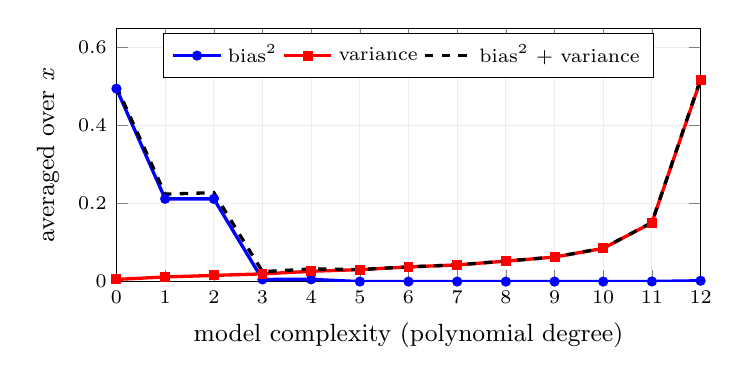
\begin{tikzpicture}
      \begin{axis}[width=9cm, height=4.8cm, xmin=0, xmax=12, ymin=0, ymax=0.65, xlabel={model complexity (polynomial degree)},
          ylabel={averaged over $x$}, tick label style={font=\scriptsize}, label style={font=\small}, xtick={0,...,12},
          legend style={font=\scriptsize, at={(0.5,0.98)}, anchor=north}, legend columns=3, grid=major, grid style={gray!15}]
        \addplot[blue, very thick, mark=*, mark size=1.2pt] coordinates {(0,0.4950) (1,0.2124) (2,0.2123) (3,0.0057) (4,0.0059) (5,0.0001) (6,0.0001) (7,0.0002) (8,0.0001) (9,0.0002) (10,0.0001) (11,0.0005) (12,0.0023)};
        \addlegendentry{bias$^2$}
        \addplot[red, very thick, mark=square*, mark size=1.2pt] coordinates {(0,0.0057) (1,0.0120) (2,0.0160) (3,0.0199) (4,0.0266) (5,0.0309) (6,0.0378) (7,0.0429) (8,0.0527) (9,0.0630) (10,0.0855) (11,0.1512) (12,0.5170)};
        \addlegendentry{variance}
        \addplot[black, very thick, dashed] coordinates {(0,0.5007) (1,0.2244) (2,0.2283) (3,0.0256) (4,0.0325) (5,0.0310) (6,0.0379) (7,0.0431) (8,0.0528) (9,0.0632) (10,0.0856) (11,0.1517) (12,0.5193)};
        \addlegendentry{bias$^2$ + variance}
      \end{axis}
    \end{tikzpicture}
    \caption{Bias--variance trade-off for polynomial regression. Many training sets $\mathcal D$ are drawn, each with $n=15$ noisy samples $f^*(x_j)+\varepsilon_j$ of $f^*(x)=\sin(2\pi x)$ at fixed positions $x_j$ (noise standard deviation $0.3$), and a polynomial $g(x;\mathcal D)$ is fitted by least squares to each. Top: $20$ fits (light red), their mean $E_{\mathcal D}\{g(x;\mathcal D)\}$ (dark red) and $f^*$ (dashed). A straight line is too rigid: all fits agree, but their mean misses $f^*$ (high bias, low variance). A degree-12 polynomial follows $f^*$ on average but varies strongly with the training set (low bias, high variance). Bottom: bias$^2$ and variance, averaged over $x$ and estimated from $400$ training sets per degree. The mean-square deviation from $f^*$ is smallest at an intermediate complexity.}
    \label{fig:bias_variance}
  \end{figure}

 \textbf {Bias-Variance Trade-Off:}
  \begin{itemize}
    \item Methods with \textbf{high flexibility} to adapt to the training data
      \begin{itemize}
        \item generally have low bias
        \item but yield high variance.            
      \end{itemize}
    \item Methods with \textbf{few parameters} and less degrees of freedom 
      \begin{itemize}
        \item tend to have a high bias, as they may not fit the data well. 
        \item However, this does not change a lot between different data sets, so these methods generally have low variance.            
      \end{itemize}
    \item Unfortunately, we can virtually never get both zero bias and zero variance!       
    \item We need to have as \textbf{much prior information} about the problem as possible to reduce both values.
  \end{itemize}
  
\subsubsection {Bias and Variance for Classification}

  Assuming a \textbf {two-class classification problem}:
  \begin{itemize}
    \item In a two-class problem, the target function changes to:
      \begin{displaymath}
        f^*(\vect x) = p(y = +1 \mid \vect x) = 1 - p(y = -1 \mid \vect x)
      \end{displaymath}
                 
    \item We cannot compare $g(\vect x ; {\mathcal{D}})$ and $f^*(\vect x)$ based on the mean-square error as in regression.
    \item For simplicity, let us assume \textbf{identical priors}: $p(y=+1)=p(y=-1)=\frac{1}{2}$.
      \begin{itemize}
        \item The Bayes-optimal prediction is $y^*(\vect x)=+1$ if $f^*(\vect x)\ge 0.5$ and $-1$ otherwise.
        \item The Bayes decision boundary is the set of points for which $f^*(\vect{x}) = 0.5$.
      \end{itemize}
  \end{itemize}
 \textbf{Boundary error}
    \begin{itemize}
    \item $p(g(\vect{x}; \mathcal{D}))$ is the density of obtaining a particular estimate of the discriminant given $\mathcal{D}$ (fixed $\vect x$, randomness comes from $\mathcal D$).
    \item Because of random variations in the training set, the boundary error depends upon this density.
  \end{itemize}

  \begin{displaymath}
    p\big(\hat y(\vect x;\mathcal D) \ne y^*(\vect x)\big) =
     \left\{
       \begin{array}{l l}
         \displaystyle{ \int_{0.5}^\infty p(g(\vect{x}; \mathcal{D})) \, \mathsf{d}g } & \mbox{if~} f^*(\vect{x}) < 0.5 \\
         \displaystyle{ \int_{-\infty}^{0.5} p(g(\vect{x}; \mathcal{D})) \, \mathsf{d}g } & \mbox{if~} f^*(\vect{x}) \ge 0.5
       \end{array}
     \right.
  \end{displaymath}

  \begin{itemize}
    \item Convenient assumption that \textbf{$p(g(\vect{x}; \mathcal{D}))$ is Gaussian}:
      \begin{eqnarray*}
        \lefteqn{p\big(\hat y(\vect x;\mathcal D) \ne y^*(\vect x)\big) =} \\
        & & \Phi \Bigg[ 
              \underbrace{\sign\left(f^*(\vect x) - \frac{1}{2}\right) \cdot \left(E_{\mathcal{D}} \{ g(\vect x ; {\mathcal{D}}) \} - \frac{1}{2}\right) }_{\mbox{\small \textbf{boundary bias}}}
              \cdot \underbrace{\mathsf{Var}_{\mathcal D}\!\Big[g(\vect x ; {\mathcal{D}})\Big]^{-1/2}}_{\mbox{\small \textbf{variance}}}
            \Bigg]
      \end{eqnarray*}
      where $\Phi$ is the \textbf{upper tail} of the standard normal:
      \begin{displaymath}
        \Phi(t) = \frac{1}{\sqrt{2\pi}} \int_t^\infty e^{-\frac{1}{2} u^2} \, \mathsf{d}u
      \end{displaymath}
    \item $p\big(\hat y(\vect x;\mathcal D) \ne y^*(\vect x)\big)$ represents the probability of incorrect estimation of the Bayes decision at $\vect x$.
  \end{itemize}
 
 \textbf{Conclusions:}

  \begin{itemize}
    \item In \textbf{regression} the bias-variance relation is additive in (bias)$^2$ and variance.     
    \item For \textbf {classification} the relation is multiplicative and nonlinear.        
    \item In classification the sign of the boundary bias affects the role of the variance in the error.            
    \item Therefore, low variance is generally important for accurate classification.
  \end{itemize}
         

 \textbf{Heuristic:} in classification, reducing the variance is often more effective than reducing the bias. This is not a theorem: the effect of bias and variance on the error depends on where the average boundary lies relative to the Bayes boundary, and neither term dominates universally.
  
  \def\covA{\mat{\Sigma}_i = \left(\begin{matrix} \sigma^2_{i1} & \sigma_{i12} \\ \sigma_{i12} & \sigma^2_{i2} \end{matrix}\right)}
  \def\covB{\mat{\Sigma}_i = \left(\begin{matrix} \sigma^2_{i1} & 0            \\ 0            & \sigma^2_{i2} \end{matrix}\right)}
  \def\covC{\mat{\Sigma}_i = \left(\begin{matrix} 1             & 0            \\ 0            & 1             \end{matrix}\right)}

\subsection{Estimating Bias and Variance}
Resampling for Estimating Statistics

 \textbf  {Problem:}
    \begin{itemize}
    \item Determine the bias and variance for some learning algorithm applied to a new problem with unknown distributions.
  \end{itemize}
   From what we have seen so far, bias and variance change with varying samples.
         

 \textbf {Resampling techniques} can be used to yield more informative estimates of a general statistics.\\
 \textbf  {Formally:}
 \begin{itemize}
    \item Suppose we want to estimate a parameter $\theta$ that depends on a random sample set $X = (x_1, \ldots, x_n)$.
    \item Assume we have an estimator $\phi_n(X)$ of $\theta$ but do not know its distribution.
   \item Resampling methods try to estimate the bias and variance of $\phi_n(X)$ using subsamples from $X$.
  \end{itemize}
  
\subsubsection{Jackknife}
  
  Let $\PS_i(X)$ be the $i$-th pseudovalue of $\phi_n(X)$:
  \begin{eqnarray*}
    \PS_i(X) 
      &=& n \phi_n(X) - (n-1) \phi_{n-1}(X_{(i)}) \\
      &=& \phi_n(X) - \underbrace{(n-1)( \phi_{n-1}(X_{(i)}) - \phi_n(X))}_{\mathsf{bias}_{\text{jack},i}}
  \end{eqnarray*}
  where $X_{(i)} = (x_1, \ldots, x_{i-1}, x_{i+1}, \ldots, x_n)$ is the set without the $i$-th element.\\
 \textbf {Notes:}
  \begin{itemize}
    \item $\PS_i(X)$ can be interpreted as a bias-corrected version of $\phi_n(X)$:        
    \item The bias trend is assumed to be in the estimators from $\phi_{n-1}(X_{(i)})$ to $\phi_n(X)$.
  \end{itemize}
 \textbf {Jackknife Principle:}
  \begin{itemize}
    \item The pseudovalues $\PS_i(X)$ are \emph{treated as if} they were independent random variables with mean $\theta$. (They are computed from overlapping leave-one-out sets and are actually dependent; the approximation works for sufficiently smooth statistics.)
    \item The jackknife estimate $\mu_{\PS}$ is approximately normal with variance $\sigma^2_{\PS}/n$.
    \item The estimators for the mean $\mu_{\PS}$ and variance $\sigma_{\PS}^2$ of the pseudovalues are the sample estimates:
      \begin{eqnarray*}
        \mu_{\PS}      &=& \frac{1}{n} \sum_{i=1}^n \PS_i(X) \\
        \sigma_{\PS}^2 &=& \frac{1}{n-1} \sum_{i=1}^n (\PS_i(X) - \mu_{\PS})^2
      \end{eqnarray*}
  \end{itemize}
 
  \begin{example}
    \small
    Estimator for the sample mean: $\phi_n(X) = \frac{1}{n} \sum_{i=1}^n x_i = \overline{X}$     Pseudovalues of $\phi_n(X)$:
    \begin{displaymath}
      \PS_i(X) = n\overline{X} - (n-1) \overline{X_{(i)}} = x_i
    \end{displaymath}
    Jackknife estimates:
    \begin{eqnarray*}
      \mu_{\PS}      &=& \frac{1}{n} \sum_{i=1}^n \PS_i(X) = \overline{X} \\
      \sigma_{\PS}^2 &=& \frac{1}{n-1} \sum_{i=1}^n (x_i - \overline{X})^2
    \end{eqnarray*}
    Estimator for sample variance: $\phi_n(X) = \frac{1}{n} \sum_{i=1}^n (x_i - \overline{X})^2$  
    Pseudovalues of $\phi_n(X)$:
    \begin{displaymath}
      \PS_i(X) = \frac{n}{n-1} (x_i - \overline{X})^2
    \end{displaymath}
    Which implies that:
    \begin{displaymath}
      \mu_{\PS} = \frac{1}{n} \sum_{i=1}^n \PS_i(X) = \frac{1}{n-1} \sum_{i=1}^n (x_i - \overline{X})^2
    \end{displaymath}
Interestingly:\\
    \begin{itemize}
      \item[ $\bullet$] $E\{\phi_n(X)\} = \frac{n-1}{n}\sigma^2$ whereas $E\{ \mu_{\PS} \} = \sigma^2$
      \item[ $\bullet$] $\mu_{\PS}$ is a bias-corrected version of $\phi_n(X)$
    \end{itemize}
  \end{example}
         
\subsubsection{Bootstrap}
  \begin{itemize}
    \item A \textit{bootstrap} data set is created by randomly selecting $n$ points from the sample set with replacement.            
    \item In \textit{bootstrap estimation} this selection process is independently repeated $B$ times.            
    \item The $B$ bootstrap data sets are treated as independent sets.
  \end{itemize}

  With $\hat\theta^{(b)}=\phi_n(X^{(b)})$ the estimate on the $b$-th bootstrap set $X^{(b)}$, $b=1,\dots,B$, the bootstrap estimate of the statistic $\theta$ and its variance are:
  \begin{eqnarray*}
    \mu_{\mathsf{BS}}      &=& \frac{1}{B} \sum_{b=1}^B \hat{\theta}^{(b)} \\
    \sigma^2_{\mathsf{BS}} &=& \frac{1}{B-1} \sum_{b=1}^B \left( \hat{\theta}^{(b)} - \mu_{\mathsf{BS}} \right)^2
  \end{eqnarray*}
  The bias is the difference between the bootstrap estimate and the estimator $\phi_n(X)$:
  \begin{displaymath}
    \mathsf{bias}_{\mathsf{BS}} = \mu_{\mathsf{BS}} - \phi_n(X)
  \end{displaymath}
 
 \textbf{Properties of the bootstrap estimate:}
  \begin{itemize}
    \item Bootstrap sets are drawn from the empirical distribution of the data (with replacement), so the class proportions are preserved in expectation.
    \item The larger the number $B$, the more the bootstrap estimate tends towards the ideal bootstrap estimate ($B\to\infty$).
    \item In contrast, the jackknife estimator requires exactly $n$ repetitions: 
      \begin{itemize}
        \item less than $n$ repetitions yield poorer estimates
        \item more than $n$ repetitions merely duplicate information already provided
      \end{itemize}
  \end{itemize}

\subsection{Estimating and Comparing Classifiers}

  Two reasons why we want to know the generalization rate of a classifier on a given problem:

  \begin{enumerate}
    \item to see if the classifier performs well enough to be useful
    \item to compare its performance with a competing design
  \end{enumerate}
\subsubsection{Cross-Validation}
  
  \begin{itemize}
    \item In \textbf{cross-validation}, the training samples are split into disjoint parts.
    \item An \textbf{$m$-fold cross-validation} splits the data into $m$ disjoint sets of size $n/m$ (here $m$ is the number of folds):
      \begin{itemize}
        \item 1 set is held out.
        \item The other $m-1$ sets are used for training.
        \item Each set is used once as held-out set.
      \end{itemize}
    \item The CV estimate is the average error over the $m$ held-out folds (weighted by fold size if folds differ in size).
    \item Note: if the held-out fold is used to stop training or to select parameters, it acts as a \textbf{validation} set and the best CV score is optimistic; the final error should be reported on separate \textbf{test} data (or with nested cross-validation).
    \item All data-dependent preprocessing (standardization, PCA, feature selection, \dots) must be fitted on the training folds only, not on the full data set.
    \item In the \textbf{extreme case of $m=n$}, we obtain a jackknife estimate of the classification accuracy.
  \end{itemize}
  The procedure is sketched in Fig.~\ref{fig:crossvalidation}.

  \begin{figure}[htbp]
    \centering
    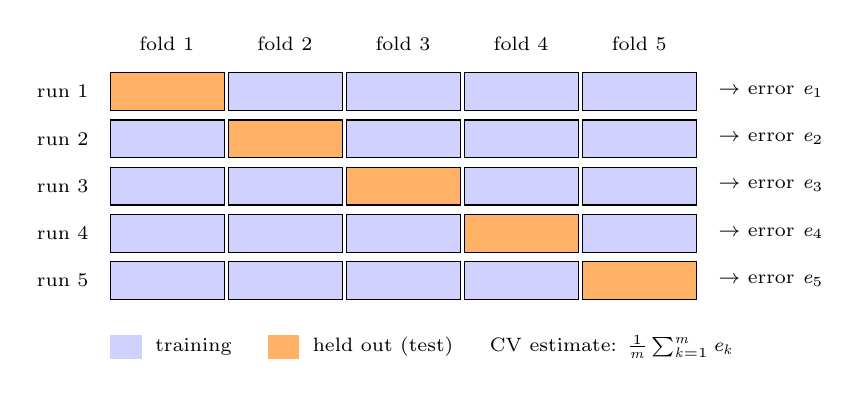
\begin{tikzpicture}[font=\small]
      \foreach \r in {1,...,5} {
        \foreach \c in {1,...,5} {
          \ifnum\r=\c \def\col{orange!60}\else\def\col{blue!18}\fi
          \fill[\col] (1.5*\c-1.5, -0.6*\r) rectangle (1.5*\c-0.05, -0.6*\r+0.48);
          \draw (1.5*\c-1.5, -0.6*\r) rectangle (1.5*\c-0.05, -0.6*\r+0.48);
        }
        \node[anchor=east, font=\scriptsize] at (-0.15, -0.6*\r+0.24) {run \r};
        \node[anchor=west, font=\scriptsize] at (7.6, -0.6*\r+0.24) {$\to$ error $e_{\r}$};
      }
      \foreach \c in {1,...,5} {\node[font=\scriptsize] at (1.5*\c-0.78, 0.25) {fold \c};}
      \fill[blue!18] (0,-3.75) rectangle (0.4,-3.45); \node[anchor=west, font=\scriptsize] at (0.45,-3.6) {training};
      \fill[orange!60] (2.0,-3.75) rectangle (2.4,-3.45); \node[anchor=west, font=\scriptsize] at (2.45,-3.6) {held out (test)};
      \node[anchor=west, font=\scriptsize] at (4.7,-3.6) {CV estimate: $\frac{1}{m}\sum_{k=1}^{m}e_k$};
    \end{tikzpicture}
    \caption{$m$-fold cross-validation with $m=5$. The data are split into $m$ disjoint folds; in run $k$, fold $k$ is held out and the classifier is trained on the other $m-1$ folds. Each sample is used exactly once for testing, and the CV estimate is the average of the $m$ held-out errors. For $m=n$ this becomes the leave-one-out (jackknife) estimate.}
    \label{fig:crossvalidation}
  \end{figure}

  For early stopping, the classifier is trained until a minimum error on a validation split (taken from the training part) is reached (good generalization vs.\ overfitting); the held-out evaluation fold must not be used for this.
   
\subsection{Lessons Learned}

  \begin{itemize}
    \item There is no such thing as a free lunch!              
    \item Bias-variance trade-off              
    \item Jackknife              
    \item Bootstrap              
    \item Cross-Validation
  \end{itemize}


\subsection{Comprehensive Questions}
 
  \begin{itemize}
    \item What is the meaning of the terms bias and variance?         
    \item What is the difference in bias-variance trade-off between regression and classification?         
    \item How do you estimate the bias and variance of a method?         
    \item What is cross-validation and how can it be used to train a classifier?
  \end{itemize}
          

\def\err{{\mathop{\overline{\mathsf{err}}}}}

\section{AdaBoost}\autocite{hastie2009,freund1997,matas,viola2001,viola2004}

\textbf{Notation in this Chapter}\\
{\small
\begin{itemize}
  \item $\mathcal D=\{(\vect x_i,y_i)\}_{i=1}^N$: training set of size $N$.
  \item $i$: sample index.
  \item $m=1,\dots,M$: boosting iteration.
  \item $y_i\in\{-1,+1\}$: true labels.
  \item $G_m(\vect x)\in\{-1,+1\}$: weak classifier in iteration $m$.
  \item $f_M(\vect x)=\sum_{m=1}^M \beta_m G_m(\vect x)$: additive model, $f_0\equiv0$; the algorithm box uses $\alpha_m=2\beta_m$, which gives the same sign.
  \item Final prediction: $\hat y = G(\vect x)=\sign(f_M(\vect x))$.
  \item $w_i^{(m)}$: weight of sample $i$ in boosting iteration $m$.
  \item $\mathbb I(\cdot)$: indicator function ($I(u,v)$ is reserved for the image intensity).
\end{itemize}
}

\subsection{Boosting methods}

  \begin{itemize}
    \item Boosting is one of the most powerful learning techniques introduced in the last twenty years.
    \item Combines output of many \textbf {\textit{weak} classifiers} to produce a powerful committee.
    \item The most popular boosting algorithm is called \textbf {\textit{AdaBoost}} \\
      (Freund and Schapire, 1997).
  \end{itemize}
\textbf{Definition:} A \textbf {weak classifier} is one whose error rate is only slightly better than random guessing.

 \subsubsection{Idea of boosting:}

  \begin{itemize}
    \item Sequentially apply the \emph{weak} classifier to repeatedly modified versions of the data.
    \item This produces a sequence of classifiers.
    \item Weighted majority vote yields the final prediction.
    \item Consider a two-class problem with $y \in \{ -1, +1\}$.          %           
    \item Given a set of observations $\mathcal{D} = \{(\vect{x}_i, y_i); \quad i=1,\ldots,N\}$ and a classifier $G(\vect x)$, the \textbf  {error rate} on the training sample is:
      \begin{displaymath}
        \err = \frac{1}{N} \sum_{i=1}^N \mathbb I(y_i \neq G(\vect{x}_i))
      \end{displaymath}
      where $\mathbb I$ is the \textbf  {indicator function}.
    \item Sequentially applied weak classifiers produce a sequence $G_m(\vect x)$ with $m=1,2,\ldots,M$ %           
    \item The \textbf{combined prediction} is then:
      \begin{displaymath}
        \hat y = G(\vect x) = \sign \left( \sum_{m=1}^M \alpha_m G_m(\vect x) \right)
      \end{displaymath}
      %           
    \item The weighting factors $\alpha_1, \ldots, \alpha_M$ are computed by the boosting algorithm. %           
    \item Each $\alpha_m$ weights the output of the corresponding classifier $G_m(\vect x)$.
  \end{itemize}

 \subsubsection{Schematic of boosting procedure:}

 \textbf{Modifications on the data:}

  \begin{itemize}
    \item Each boosting step consists of applying weights $w_1, w_2, \ldots, w_N$ to the training samples.
    \item Initially, the weights are set to $w_i = 1/N$.
    \item Thus the first classifier in the sequence is trained the usual way. %           
    \item For $m \geq 2$ the weights are individually modified. %           
    \item The classifiers $G_m$, with $m \geq 2$ are trained on differently-weighted samples.
  \end{itemize}
 
 \textbf {Weighting scheme:}
  \begin{itemize}
    \item At step $m$ the misclassified observations from $G_{m-1}$ have increased weights.
    \item The weights for correctly classified samples from $G_{m-1}$ have decreased weights.
  \end{itemize}
         

 \textbf {Effects of the weighting scheme:}
  \begin{itemize}
    \item Observations that are difficult to classify correctly get ever-increasing influence.
    \item Each successive classifier is forced to concentrate more on those observations that were misclassified by the previous one.
  \end{itemize}
 
\subsection{AdaBoost}

 \textbf {AdaBoost algorithm:}
%
  \begin{centernss}
    \small
      \begin{struktogramm}(100,62)\\
        \assign{Initialize weights: $w_i \gets 1/N ~,~ i=1, \ldots, N$}
        \assign{$m \gets 1$}
        \until{$m > M$}\\
          \assign{{Fit classifier $G_m(\vect x)$ to training data using weights $w_1,\dots,w_N$}}\\
          \assign{{Compute classification error:}\\
            $ \mathsf{err}_m = \frac{\sum_{i=1}^N w_i \mathbb I(y_i \neq G_m(\vect x_i))}{\sum_{i=1}^N w_i}$
          }\\
          \assign{{Compute classifier weights:}\\
            $ \alpha_m = \log \left( \frac{1- \mathsf{err}_m}{\mathsf{err}_m} \right) $
          }\\
          \assign{{Compute new sample weights:}\\
            $ w_i \leftarrow w_i \exp \left[ \alpha_m \mathbb I(y_i \neq G_m(\vect x_i)) \right] ~,~ i = 1, \ldots, N $
          }
          \assign{$m \gets m + 1$}\\
        \untilend
        \assign{\textbf{Output:} $\hat y = G(\vect x) = \sign \left( \sum_{m=1}^M \alpha_m G_m(\vect x) \right) $}
      \end{struktogramm}
    
  \end{centernss}
 \textbf {Notes:}
  \begin{itemize}
    \item This version of AdaBoost is called \textbf {discrete}, because each $G_m(\vect x)$ returns a discrete class label. %           
    \item AdaBoost can be modified to return also a real-valued prediction in the interval $[-1,+1]$.  % 
    \item Instead of taking just any classifier for $G_m(\vect x)$, that classifier may be used that results in the smallest error at step $m$.
  \end{itemize}

  AdaBoost dramatically increases the performance of even a very weak classifier.
 
\subsection{Exponential Loss}

  \begin{itemize}
    \item Boosting fits an \textbf{additive model} in a \textbf{set of elementary basis functions}:
      \begin{displaymath}
        f(\vect x)=\sum_{m=1}^{M} \beta_m\, b(\vect x;\vect\gamma_m),
      \end{displaymath}
      where $\beta_m$ are expansion coefficients and $b(\vect x;\vect \gamma_m)$ is a basis function with parameters $\vect \gamma_m$.
    \item Additive expansions are very popular in learning techniques:
      \begin{itemize}
        \item single-hidden-layer neural networks (perceptron)
        \item wavelets
        \item classification trees
        \item etc.
      \end{itemize}
  \end{itemize}
  
  \begin{itemize}
    \item Expansion models are typically fit by \textbf{minimizing a loss function $L$} averaged over the training data:
      \begin{equation} 
        \label{eq:loss}
        \min_{\{ \beta_m, \vect \gamma_m \}_1^M } ~ 
        \left\{
          \sum_{i=1}^N L \big( y_i, f_M(\vect{x}_i) \big) =
          \sum_{i=1}^N L \left( y_i, \sum_{m=1}^M \beta_m \, b(\vect{x}_i ; \vect \gamma_m) \right)
        \right\}
      \end{equation}
                           
    \item\textbf  {Forward stagewise modeling} approximates the solution to \eqref{eq:loss}:
      \begin{itemize}
        \item New basis functions are sequentially added.          
        \item Parameters and coefficients of already added functions are not changed.
        \item At each iteration, the subproblem of fitting just a single basis function is solved.
      \end{itemize}
  \end{itemize}
          
  \begin{itemize}
    \item The \textbf {$m$-th subproblem} may be rewritten as:              
      \begin{center}
            $
              \displaystyle
              (\beta_m, \vect \gamma_m) = \argmin_{\beta, \vect \gamma} ~\sum_{i=1}^N L\big(y_i, f_{m-1}(\vect{x}_i) + \beta \, b(\vect{x}_i ; \vect{\gamma})\big)
            $
      \end{center}
    \item AdaBoost is equivalent to a forward stagewise additive modeling using an \textbf {exponential loss function}:
      \begin{displaymath}
        L(y, f(\vect x)) = \exp (-y \, f(\vect x))
      \end{displaymath}
  \end{itemize}
  \textbf {Proof:}

  \begin{itemize}
    \item For AdaBoost, the basis functions are the classifiers $G_m(\vect x) \in \{-1,+1\}$.
    \item Using the \textbf{exponential loss function}, one must solve at each step:
      \begin{eqnarray*}
        (\beta_m, G_m) = \argmin_{\beta, G} ~\sum_{i=1}^N \exp \left[ -y_i \big(f_{m-1}(\vect{x}_i) + \beta G(\vect{x}_i)\big) \right]
      \end{eqnarray*}
    \item Using the weight $w_i^{(m)} = \exp(-y_i \, f_{m-1}(\vect{x}_i))$ (so $w_i^{(1)}=1$ since $f_0\equiv0$) this can be rewritten as:
      \begin{eqnarray*}
        (\beta_m, G_m) = \argmin_{\beta, G} ~\sum_{i=1}^N w_i^{(m)} \exp (-\beta y_i G(\vect{x}_i))
      \end{eqnarray*}
  \end{itemize}

 \textbf {Observations:}
  \begin{itemize}
    \item Since $w_i^{(m)}$ is independent of $\beta$ and $G(\vect x)$, it can be seen as a weight applied to each observation.
    \item However, this weight depends on $f_{m-1}$, so the weights change with each iteration $m$.
  \end{itemize}

  \begin{eqnarray*}
    (\beta_m, G_m) 
      &=& \argmin_{\beta, G} ~\sum_{i=1}^N w_i^{(m)} \exp (-\beta y_i G(\vect{x}_i)) \\ 
      &=& \argmin_{\beta, G} ~ e^{-\beta} \sum_{y_i = G(\vect{x}_i)} w_i^{(m)} + e^{\beta} \sum_{y_i \neq G(\vect{x}_i)} w_i^{(m)} \\ 
      &=& \argmin_{\beta, G} ~ \left( e^{\beta} - e^{-\beta} \right) \sum_{i=1}^N w_i^{(m)} \mathbb I(y_i \neq G(\vect{x}_i)) + e^{-\beta} \sum_{i=1}^N w_i^{(m)}
  \end{eqnarray*}

  \begin{itemize}
    \item The weight scaling is irrelevant for selecting $G_m$ (positive scaling does not change the argmin).
    \item Plugging the optimal $G_m(\vect x)$ into the objective function and solving for $\beta_m$: with the \textbf{minimized weighted error rate}
      \begin{displaymath}
        \mathsf{err}_m = \frac{\sum_{i=1}^N w_i^{(m)} \mathbb I(y_i \neq G_m(\vect{x}_i))}{\sum_{i=1}^N w_i^{(m)}}
      \end{displaymath}
      the objective (divided by $\sum_i w_i^{(m)}$) is $(e^{\beta}-e^{-\beta})\,\mathsf{err}_m+e^{-\beta}$. Setting its derivative to zero gives $(e^{\beta}+e^{-\beta})\,\mathsf{err}_m=e^{-\beta}$, i.\,e.\ $e^{2\beta}=\frac{1-\mathsf{err}_m}{\mathsf{err}_m}$:
      \begin{displaymath}
        \beta_m=\frac12\log\frac{1-\mathsf{err}_m}{\mathsf{err}_m}.
      \end{displaymath}
     \item From the update formula of the approximation:
      \begin{eqnarray*}
        f_m(\vect x) = f_{m-1}(\vect x) + \beta_m \, G_m(\vect x)
      \end{eqnarray*}
      we can calculate the \textbf{weights for the next iteration}:
      \begin{align*}
        w_i^{(m+1)}
          &= w_i^{(m)} \, e^{-\beta_m y_i G_m(\vect{x}_i)} \\
          &\qquad \text{(using: $-y_i G_m(\vect{x}_i) = 2 \mathbb I(y_i \neq G_m(\vect{x}_i)) - 1$)} \\
          &= w_i^{(m)} \, e^{\alpha_m \mathbb I(y_i \neq G_m(\vect{x}_i))} \, e^{-\beta_m}
      \end{align*}
      with $\alpha_m = 2 \beta_m$ and thus $\hat y = \sign(f_M(\vect x))$.
  \end{itemize}
 

 \textbf {Compare result to initial AdaBoost algorithm:}

  \begin{itemize}
    \item\textbf {Exponential loss:}
      \begin{eqnarray*}
        \beta_m     &=& \frac{1}{2} \log \frac{1 - \mathsf{err}_m}{\mathsf{err}_m} \\
        \alpha_m    &=& 2 \beta_m \\
        w_i^{(m+1)} &=& w_i^{(m)} ~ e^{\alpha_m \mathbb I(y_i \neq G_m(\vect{x}_i))} ~ e^{-\beta_m}
      \end{eqnarray*}
             
    \item\textbf {AdaBoost:}
      \begin{eqnarray*}
        \alpha_m &=&          \log \frac{1- \mathsf{err}_m}{\mathsf{err}_m} \\
        w_i      &\leftarrow& w_i \, e^{\alpha_m \mathbb I(y_i \neq G_m(\vect{x}_i))}
      \end{eqnarray*}
  \end{itemize}
          


 
 \textbf {Discussion:}

  \begin{itemize}
    \item The equivalence of AdaBoost to forward stagewise additive modeling was discovered five years after its invention. %           
    \item The AdaBoost criterion yields a monotone decreasing function of the \textbf        {margin}: $y\,f(\vect x)$.          %           
    \item In $\{-1, +1\}$ classification, the margin plays a role similar to the \\
      residuals $y - f(\vect x)$ in regression:
      \begin{itemize}
        \item Observations with $y_i \, f(\vect{x}_i) > 0$ are classified correctly
        \item Observations with $y_i \, f(\vect{x}_i) < 0$ are misclassified 
        \item The decision boundary is at $f(\vect x) = 0$
     \end{itemize}
   \item The goal of the classification algorithm is to produce positive margins as frequently as possible. % 
    \item Thus, any loss criterion should penalize negative margins more heavily than positive ones! % 
    \item The exponential criterion concentrates much more influence on observations with large negative margins.
  \end{itemize}
 
  Due to the exponential loss, AdaBoost performance is known to degrade rapidly:
  \begin{itemize}
    \item in situations of noisy data
    \item when there are wrong class labels in the training data
  \end{itemize}
 
\subsection{Face Detection}

  Famous algorithm developed by \textbf {Viola and Jones} in 2001.
 \textbf{Contributions:}

  \begin{itemize}
    \item Integral images for feature computation.
    \item Usage of AdaBoost for boosting.
    \item Classifier cascade for fast rejection of non-face regions.
  \end{itemize}

  Various implementations available: for example look into \textit{OpenCV FaceDetector} sample code.
 
 \textbf{Features:}

  \begin{itemize}
    \item Features are adapted from Haar basis functions. %           
    \item They are calculated by subtracting the sum of the pixels in the white from the sum of the pixels in the gray rectangles:               %           
  \end{itemize}

 4 types of features used (Fig.~\ref{fig:vj_haar}):
  \begin{itemize}
    \item The exhaustive set of Haar-like rectangle features is very large (in the classic Viola--Jones setup this count refers to the $24\times 24$ detection window, not to the full image). %
    \item Rectangle features can be efficiently computed using an \\
    \textbf {Integral Image $II$}:
      \begin{displaymath}
        II(u,v) = \sum_{u' \leq u, v' \leq v} I(u', v')
      \end{displaymath}
      where $I(u',v')$ is the image intensity at pixel $(u',v')$ (pixel coordinates $(u,v)$, since $\vect x$ denotes the image sub-window).
  \end{itemize}

The sum of intensities over any rectangle needs only four look-ups in the integral image (three additions/subtractions); see Fig.~\ref{fig:vj_integral}.\\

  \begin{figure}[htbp]
    \centering
    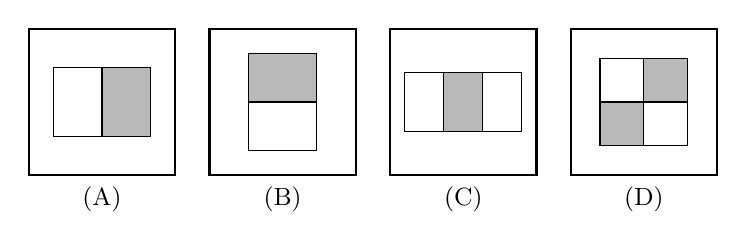
\begin{tikzpicture}[scale=0.62, font=\small]
      \tikzset{win/.style={draw, thick}, gr/.style={fill=gray!55, draw}, wh/.style={fill=white, draw}}
      % (A) two-rectangle, horizontal
      \begin{scope}
        \draw[win] (0,0) rectangle (3,3);
        \draw[wh] (0.5,0.8) rectangle (1.5,2.2); \draw[gr] (1.5,0.8) rectangle (2.5,2.2);
        \node at (1.5,-0.5) {(A)};
      \end{scope}
      % (B) two-rectangle, vertical
      \begin{scope}[xshift=3.7cm]
        \draw[win] (0,0) rectangle (3,3);
        \draw[gr] (0.8,1.5) rectangle (2.2,2.5); \draw[wh] (0.8,0.5) rectangle (2.2,1.5);
        \node at (1.5,-0.5) {(B)};
      \end{scope}
      % (C) three-rectangle
      \begin{scope}[xshift=7.4cm]
        \draw[win] (0,0) rectangle (3,3);
        \draw[wh] (0.3,0.9) rectangle (1.1,2.1); \draw[gr] (1.1,0.9) rectangle (1.9,2.1); \draw[wh] (1.9,0.9) rectangle (2.7,2.1);
        \node at (1.5,-0.5) {(C)};
      \end{scope}
      % (D) four-rectangle
      \begin{scope}[xshift=11.1cm]
        \draw[win] (0,0) rectangle (3,3);
        \draw[wh] (0.6,1.5) rectangle (1.5,2.4); \draw[gr] (1.5,1.5) rectangle (2.4,2.4);
        \draw[gr] (0.6,0.6) rectangle (1.5,1.5); \draw[wh] (1.5,0.6) rectangle (2.4,1.5);
        \node at (1.5,-0.5) {(D)};
      \end{scope}
    \end{tikzpicture}
    \caption{The four types of Haar-like rectangle features inside the detection window: two-rectangle features (A, B), a three-rectangle feature (C) and a four-rectangle feature (D). The feature value $\phi_j(\vect x)$ is the sum of the pixel intensities in the gray rectangles minus the sum in the white rectangles. Position, size and type of the rectangles are varied over the whole $24\times24$ window, which gives the very large set of candidate features from which AdaBoost selects.}
    \label{fig:vj_haar}
  \end{figure}

  \begin{figure}[htbp]
    \centering
    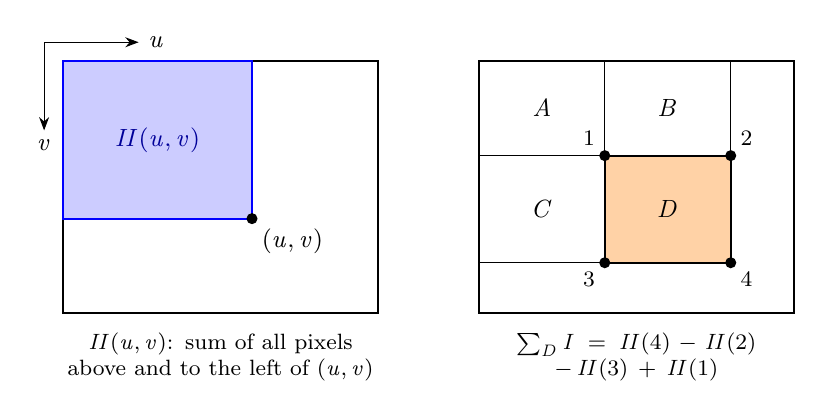
\begin{tikzpicture}[scale=0.8, font=\small, >={Stealth}]
      % left: definition of II(u,v)
      \begin{scope}
        \draw[thick] (0,0) rectangle (5,4);
        \fill[blue!20] (0,4) rectangle (3,1.5);
        \draw[blue, thick] (0,4) rectangle (3,1.5);
        \fill (3,1.5) circle (2.5pt) node[below right] {$(u,v)$};
        \node[blue!60!black, align=center] at (1.5,2.75) {$II(u,v)$};
        \draw[->] (-0.3,4.3) -- (1.2,4.3) node[right] {$u$};
        \draw[->] (-0.3,4.3) -- (-0.3,2.9) node[below] {$v$};
        \node[align=center, font=\footnotesize, text width=4.2cm] at (2.5,-0.7) {$II(u,v)$: sum of all pixels above and to the left of $(u,v)$};
      \end{scope}
      % right: rectangle sum with four look-ups
      \begin{scope}[xshift=6.6cm]
        \draw[thick] (0,0) rectangle (5,4);
        \draw (0,4) rectangle (2,2.5); \node at (1,3.25) {$A$};
        \draw (2,4) rectangle (4,2.5); \node at (3,3.25) {$B$};
        \draw (0,2.5) rectangle (2,0.8); \node at (1,1.65) {$C$};
        \fill[orange!35] (2,2.5) rectangle (4,0.8); \draw[thick] (2,2.5) rectangle (4,0.8); \node at (3,1.65) {$D$};
        \foreach \p/\n/\a in {(2,2.5)/1/above left, (4,2.5)/2/above right, (2,0.8)/3/below left, (4,0.8)/4/below right}
          {\fill \p circle (2.5pt) node[\a, font=\footnotesize] {\n};}
        \node[align=center, font=\footnotesize, text width=4.2cm] at (2.5,-0.7) {$\sum_D I = II(4)-II(2)$\\$-\,II(3)+II(1)$};
      \end{scope}
    \end{tikzpicture}
    \caption{Integral image. Left: $II(u,v)$ stores the sum of all intensities $I(u',v')$ with $u'\le u$, $v'\le v$; it is computed in one pass over the image. Right: with the corner values $II(1)=A$, $II(2)=A+B$, $II(3)=A+C$ and $II(4)=A+B+C+D$ (letters denoting region sums), the sum over any rectangle $D$ needs only four look-ups: $D=II(4)-II(2)-II(3)+II(1)$. A rectangle feature therefore costs a constant number of operations, independent of its size.}
    \label{fig:vj_integral}
  \end{figure}
 \textbf {Boosting:}\\

  \begin{itemize}
    \item The classification functions are restricted to each depend on a single feature only. %           
    \item This way, AdaBoost can be interpreted as an effective feature selecting algorithm:
      \begin{itemize}
        \item The single rectangle feature is selected which best separates the observations. %  
        \item For each feature, the weak learner determines the optimal threshold classification function.
      \end{itemize}
     \item A weak classifier $G_j(\vect x)$ consists of a \textbf{feature value $\phi_j(\vect x)$} ($j$: feature index), an \textbf {optimal threshold $\theta_j$}, and a \textbf{parity $s_j$} to indicate the direction of the inequality:
      \begin{displaymath}
        G_j(\vect x) = \begin{cases}
                        +1 \quad \mbox{if} ~s_j \phi_j(\vect x) < s_j \theta_j \\
                        -1 \quad \mbox{otherwise}
                      \end{cases}
      \end{displaymath}
      with $\vect x$ being a sub-window of an image. (Viola and Jones use $G_j\in\{0,1\}$ and decide ``face'' iff $\sum_m\alpha_m G_m\ge\frac12\sum_m\alpha_m$; with $\pm1$ outputs this is the sign rule above.)
    \item Very aggressive process to discard the vast majority of features.
 \item The best features selected by AdaBoost are shown in the slides.
  \end{itemize}
 \textbf {Classifier Cascade:}

  \begin{itemize}
    \item Despite the efficiency of the feature computation, the complexity of the problem is still huge. %           
    \item Evaluating the full AdaBoost sequence on all sub-windows of the image takes too much time.
    \item Idea of cascaded classifiers:
    \begin{itemize}
      \item Simpler classifiers used to reject the majority of sub-windows. %           
      \item Each stage is again created by AdaBoost. %           
      \item Stage 1 uses the two best features; it detects 100\,\% of the faces (true positive rate, TPR) with a false positive rate (FPR) of around 40\,\% (rates as defined in Chapter~1).
    \end{itemize}
  \end{itemize}

  \begin{itemize}
    \item The cascade has the overall shape of a degenerated decision tree (Fig.~\ref{fig:vj_cascade}):         
    \item A negative classification at any stage yields an immediate rejection of the sub-window.
    \item Structure of cascade reflects the (usually) overwhelming majority of negative sub-windows in an image. %           
    \item Goal is to reject as many negatives as possible at the earliest stage of the processing.
  \end{itemize}

  \begin{figure}[htbp]
    \centering
    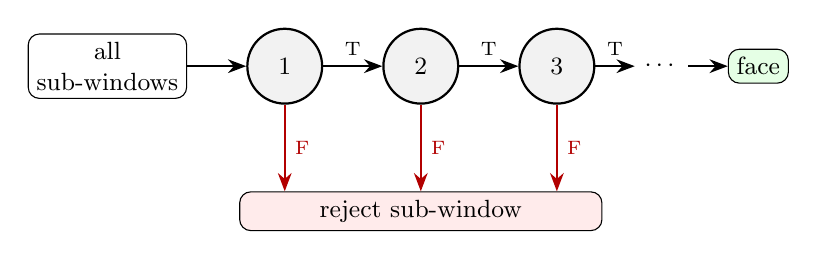
\begin{tikzpicture}[font=\small, >={Stealth}, node distance=0.6cm and 0.75cm,
        st/.style={draw, thick, circle, minimum size=0.95cm, fill=gray!10, align=center, inner sep=1pt},
        io/.style={draw, rounded corners, align=center, inner sep=3pt}]
      \node[io] (in) {all\\sub-windows};
      \node[st, right=of in] (s1) {1};
      \node[st, right=of s1] (s2) {2};
      \node[st, right=of s2] (s3) {3};
      \node[right=0.5cm of s3] (dots) {$\cdots$};
      \node[io, right=0.5cm of dots, fill=green!10] (out) {face};
      \node[io, below=1.1cm of s2, fill=red!8, minimum width=4.6cm] (rej) {reject sub-window};
      \draw[->, thick] (in) -- (s1);
      \draw[->, thick] (s1) -- node[above, font=\scriptsize] {T} (s2);
      \draw[->, thick] (s2) -- node[above, font=\scriptsize] {T} (s3);
      \draw[->, thick] (s3) -- node[above, font=\scriptsize] {T} (dots);
      \draw[->, thick] (dots) -- (out);
      \foreach \s in {s1,s2,s3} {\draw[->, thick, red!70!black] (\s) -- node[right, font=\scriptsize] {F} (\s |- rej.north);}
    \end{tikzpicture}
    \caption{Attentional cascade. Each stage is a boosted classifier tuned for a very high detection rate. A sub-window is passed on only if a stage accepts it (T); any rejection (F) discards it immediately. Since the vast majority of sub-windows contain no face, most of them are rejected by the first, very cheap stages (stage 1 uses only two features), and only the few face-like windows reach the expensive later stages. The overall rates are the products of the stage rates, e.\,g.\ with $10$ stages of TPR $0.99$ and FPR $0.3$: TPR $\approx0.99^{10}\approx0.90$, FPR $\approx0.3^{10}\approx6\cdot10^{-6}$.}
    \label{fig:vj_cascade}
  \end{figure}
  
 \textbf {Training of the cascade:}

  \begin{itemize}
    \item Subsequent classifiers are trained using only those examples which pass through all the previous stages. %           
    \item The next classifier faces a more difficult task than the previous one. 
    \item Trade-off between more features achieving higher detection rates and lower false positive rates while requiring more computation time.
  \end{itemize}
 \textbf {Final classifier:}
refer to slides for more details. 
  \begin{itemize}
    \setlength\itemsep{0.5cm}
    \item 32 layer cascade of increasingly strong boosted classifiers
    
    \begin{center}
      \begin{tabular}{r@{}l r c c}
        \multicolumn{2}{c}{\structure{Layer}} & 
       \textbf        {\# Features} & 
       \textbf        {TPR} &
       \textbf        {FPR}\\
        \hline
           &1  &   2~~~~~ & 100\,\% & 40\,\% \\
           &2  &   5~~~~~ & 100\,\% & 20\,\% \\
         3-&5  &  20~~~~~ & \\
         6-&7  &  50~~~~~ & \\
         8-&12 & 100~~~~~ & \\
        13-&32 & 200~~~~~ & \\ %           
      \end{tabular}
    \end{center}

    \item Number of stages and features adapted until false positive rate on validation was nearly zero while maintaining high correct rate.
  \end{itemize}

\subsection{Lessons Learned}

  \begin{itemize}
    \item Boosting of weak classifiers can yield a powerful combined classifier          
    \item AdaBoost algorithm              
    \item Weights of the classifiers and on the data are adjusted              
    \item AdaBoost minimizes an exponential loss function
    \item Viola \& Jones face detection algorithm
  \end{itemize}


          

\newpage
\printbibliography

\end{document}

